% SPDX-License-Identifier: GPL-3.0-or-later
\chapter{Steaua Noastră, Planetele și Sateliții Lor Naturali}
\label{chap:planete}

Sistemul nostru Solar s-a format acum aproximativ \textbf{4,6 miliarde de ani} din prăbușirea gravitațională a unui nor molecular gigant de gaz și praf interstelar. Peste $99{,}86\%$ din întreaga masă a sistemului s-a concentrat în centru, dând naștere stelei noastre, \textbf{Soarele}, în timp ce din discul protoplanetar rămas s-au format \textbf{cele 8 planete majore} și \textbf{sateliții lor naturali (lunile)}, care sunt prezentate în acest capitol împreună cu planeta în jurul căreia orbitează:
\begin{enumerate}[leftmargin=1.6em, itemsep=2pt]
  \item \textbf{Planetele Interioare Telurice (Stâncoase):} \emph{Mercur} și \emph{Venus} (fără sateliți naturali), \emph{Pământul} (însoțit de \emph{Lună}) și \emph{Marte} (însoțit de sateliții săi capturați \emph{Phobos} și \emph{Deimos}).
  \item \textbf{Planetele Exterioare Gigante și Sistemele Lor de Sateliți:} \emph{Giganții Gazoși}, reprezentați de \emph{Jupiter} (cu cele 4 luni galileene: \emph{Io, Europa, Ganymede, Callisto}) și \emph{Saturn} (cu \emph{Mimas, Enceladus, Tethys, Dione, Rhea, Titan, Hyperion, Iapetus, Phoebe}), precum și \emph{Giganții de Gheață}, reprezentați de \emph{Uranus} (cu \emph{Miranda, Ariel, Umbriel, Titania, Oberon}) și \emph{Neptun} (cu satelitul retrograd \emph{Triton}).
\end{enumerate}

\begin{center}
\resizebox{\textwidth}{!}{%
\begin{tikzpicture}[scale=0.88, every node/.style={transform shape}]
  \fill[orbitarSpaceBg, rounded corners=6pt] (-0.8,-1.8) rectangle (15.6,2.1);
  % Soarele
  \shade[inner color=yellow!95!white, outer color=orange!90!red] (0.2,0) circle (0.72cm);
  \node[white, font=\scriptsize\bfseries] at (0.2,-1.15) {Soarele};

  % Mercur
  \fill[gray!70] (1.7,0) circle (0.10cm);
  \node[white, font=\scriptsize] at (1.7,0.55) {Mercur};
  \node[orbitarCyan, font=\tiny] at (1.7,-0.55) {0,39 UA};

  % Venus
  \fill[yellow!75!orange] (3.0,0) circle (0.18cm);
  \node[white, font=\scriptsize] at (3.0,0.65) {Venus};
  \node[orbitarCyan, font=\tiny] at (3.0,-0.55) {0,72 UA};

  % Pământ
  \fill[cyan!70!blue] (4.4,0) circle (0.19cm);
  \node[white, font=\scriptsize\bfseries] at (4.4,0.65) {Pământ};
  \node[orbitarCyan, font=\tiny] at (4.4,-0.55) {1,00 UA};

  % Marte
  \fill[orange!85!red] (5.8,0) circle (0.14cm);
  \node[white, font=\scriptsize] at (5.8,0.60) {Marte};
  \node[orbitarCyan, font=\tiny] at (5.8,-0.55) {1,52 UA};

  % Centura de asteroizi
  \draw[gray!60, line width=2.2pt, dotted] (6.9,-1.3) -- (6.9,1.3);
  \node[gray!40, font=\tiny, rotate=90] at (6.65,0) {Centura de Asteroizi};

  % Jupiter
  \fill[orange!65!brown] (8.3,0) circle (0.50cm);
  \node[white, font=\scriptsize\bfseries] at (8.3,0.88) {Jupiter};
  \node[orbitarCyan, font=\tiny] at (8.3,-0.85) {5,20 UA};

  % Saturn
  \fill[yellow!70!brown] (10.4,0) circle (0.42cm);
  \draw[white!80, line width=1.2pt] (10.4,0) ellipse (0.72cm and 0.18cm);
  \node[white, font=\scriptsize\bfseries] at (10.4,0.85) {Saturn};
  \node[orbitarCyan, font=\tiny] at (10.4,-0.80) {9,58 UA};

  % Uranus
  \fill[cyan!60!white] (12.5,0) circle (0.28cm);
  \node[white, font=\scriptsize] at (12.5,0.72) {Uranus};
  \node[orbitarCyan, font=\tiny] at (12.5,-0.68) {19,20 UA};

  % Neptun
  \fill[blue!70!cyan] (14.3,0) circle (0.27cm);
  \node[white, font=\scriptsize] at (14.3,0.72) {Neptun};
  \node[orbitarCyan, font=\tiny] at (14.3,-0.68) {30,07 UA};
\end{tikzpicture}%
}
\end{center}

\begin{table}[H]
\centering
\small
\caption{Tabel sinoptic comparativ: Soarele și cele 8 planete ale Sistemului Solar în Orbitar}
\resizebox{\textwidth}{!}{%
\begin{tabular}{@{}llrrrrr@{}}
\toprule
\textbf{Corp ceresc} & \textbf{Clasă} & \textbf{Distanță (UA)} & \textbf{Rază (km)} & \textbf{Masă ($M_\oplus$)} & \textbf{Gravitație ($g_\oplus$)} & \textbf{Temp. medie} \\
\midrule
Soarele & Stea (G2V) & 0,00 & 696.340 & 332946,00 & 27,94 & 5.505$^\circ$C \\
Mercur & Telurică & 0,39 & 2.439,7 & 0,06 & 0,38 & 167$^\circ$C \\
Venus & Telurică & 0,72 & 6.051,8 & 0,81 & 0,90 & 464$^\circ$C \\
Pământul & Telurică & 1,00 & 6.371 & 1,00 & 1,00 & 15$^\circ$C \\
Marte & Telurică & 1,52 & 3.389,5 & 0,11 & 0,38 & -63$^\circ$C \\
Jupiter & Gigant gazos & 5,20 & 69.911 & 317,80 & 2,53 & -110$^\circ$C \\
Saturn & Gigant gazos & 9,58 & 58.232 & 95,16 & 1,06 & -140$^\circ$C \\
Uranus & Gigant gheață & 19,22 & 25.362 & 14,54 & 0,89 & -195$^\circ$C \\
Neptun & Gigant gheață & 30,11 & 24.622 & 17,15 & 1,14 & -200$^\circ$C \\
\bottomrule
\end{tabular}%
}
\end{table}

\begin{table}[H]
\centering
\small
\caption{Tabel sinoptic al celor 23 de sateliți naturali majori din Orbitar (asociați cu planetele lor)}
\resizebox{\textwidth}{!}{%
\begin{tabular}{@{}llrrrr@{}}
\toprule
\textbf{Satelit (Lună)} & \textbf{Planeta-mamă} & \textbf{Rază (km)} & \textbf{Gravitație ($g_\oplus$)} & \textbf{Perioadă orbitală} & \textbf{Temp. medie} \\
\midrule
Luna & Pământul & 1737,4 & 0,165 & 27,32 zile & -23$^\circ$C \\
Phobos & Marte & 11,3 & 0,001 & 0,32 zile & -40$^\circ$C \\
Deimos & Marte & 6,2 & 0,000 & 1,26 zile & -40$^\circ$C \\
Io & Jupiter & 1821,6 & 0,183 & 1,77 zile & -143$^\circ$C \\
Europa & Jupiter & 1560,8 & 0,134 & 3,55 zile & -160$^\circ$C \\
Ganymede & Jupiter & 2631,2 & 0,146 & 7,16 zile & -163$^\circ$C \\
Callisto & Jupiter & 2410,3 & 0,126 & 16,69 zile & -139$^\circ$C \\
Mimas & Saturn & 198,2 & 0,006 & 0,94 zile & -209$^\circ$C \\
Enceladus & Saturn & 252,1 & 0,011 & 1,37 zile & -198$^\circ$C \\
Tethys & Saturn & 531,1 & 0,015 & 1,89 zile & -187$^\circ$C \\
Dione & Saturn & 561,4 & 0,024 & 2,74 zile & -186$^\circ$C \\
Rhea & Saturn & 763,8 & 0,027 & 4,52 zile & -197$^\circ$C \\
Titan & Saturn & 2574,7 & 0,138 & 15,95 zile & -179$^\circ$C \\
Hyperion & Saturn & 135,0 & 0,002 & 21,28 zile & -180$^\circ$C \\
Iapetus & Saturn & 734,5 & 0,023 & 79,32 zile & -163$^\circ$C \\
Phoebe & Saturn & 106,5 & 0,004 & 550,31 zile (retrograd) & -198$^\circ$C \\
Miranda & Uranus & 235,8 & 0,008 & 1,41 zile & -213$^\circ$C \\
Ariel & Uranus & 578,9 & 0,025 & 2,52 zile & -213$^\circ$C \\
Umbriel & Uranus & 584,7 & 0,023 & 4,14 zile & -198$^\circ$C \\
Titania & Uranus & 788,4 & 0,039 & 8,71 zile & -203$^\circ$C \\
Oberon & Uranus & 761,4 & 0,035 & 13,46 zile & -198$^\circ$C \\
Triton & Neptun & 1353,4 & 0,079 & 5,88 zile (retrograd) & -235$^\circ$C \\
Charon & Pluto & 606,0 & 0,029 & 6,39 zile & -220$^\circ$C \\
\bottomrule
\end{tabular}%
}
\end{table}

\clearpage

\section{Soarele}
\label{sec:body-sun}
\vspace{-4pt}
{\large\itshape\color{orbitarAccent} Steaua centrală a Sistemului Solar (Pitică Galbenă G2V)}\\[4pt]


\begin{center}
\begin{tabular}{@{}m{0.44\textwidth}@{\hspace{0.03\textwidth}}m{0.51\textwidth}@{}}
\centering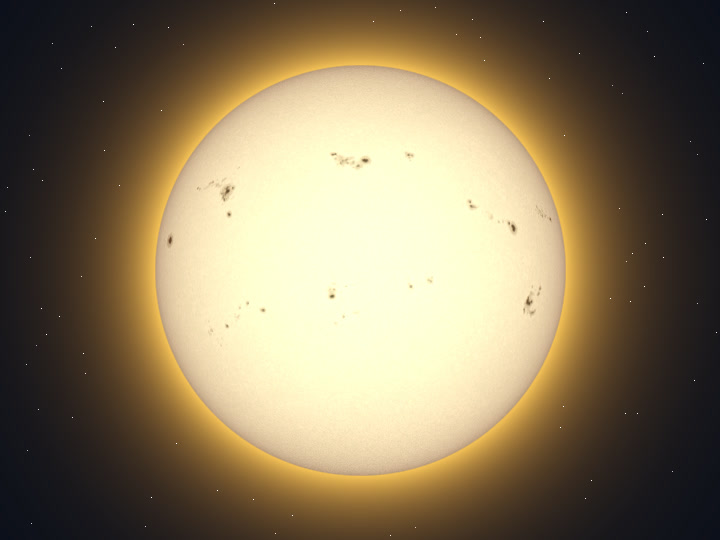
\includegraphics[width=\linewidth,height=4.4cm,keepaspectratio]{imagini/globuri/sun.jpg}\\[2pt]
{\scriptsize\itshape\color{orbitarMuted} Vedere 3D a corpului ceresc (\textbf{Soarele})}
&
\centering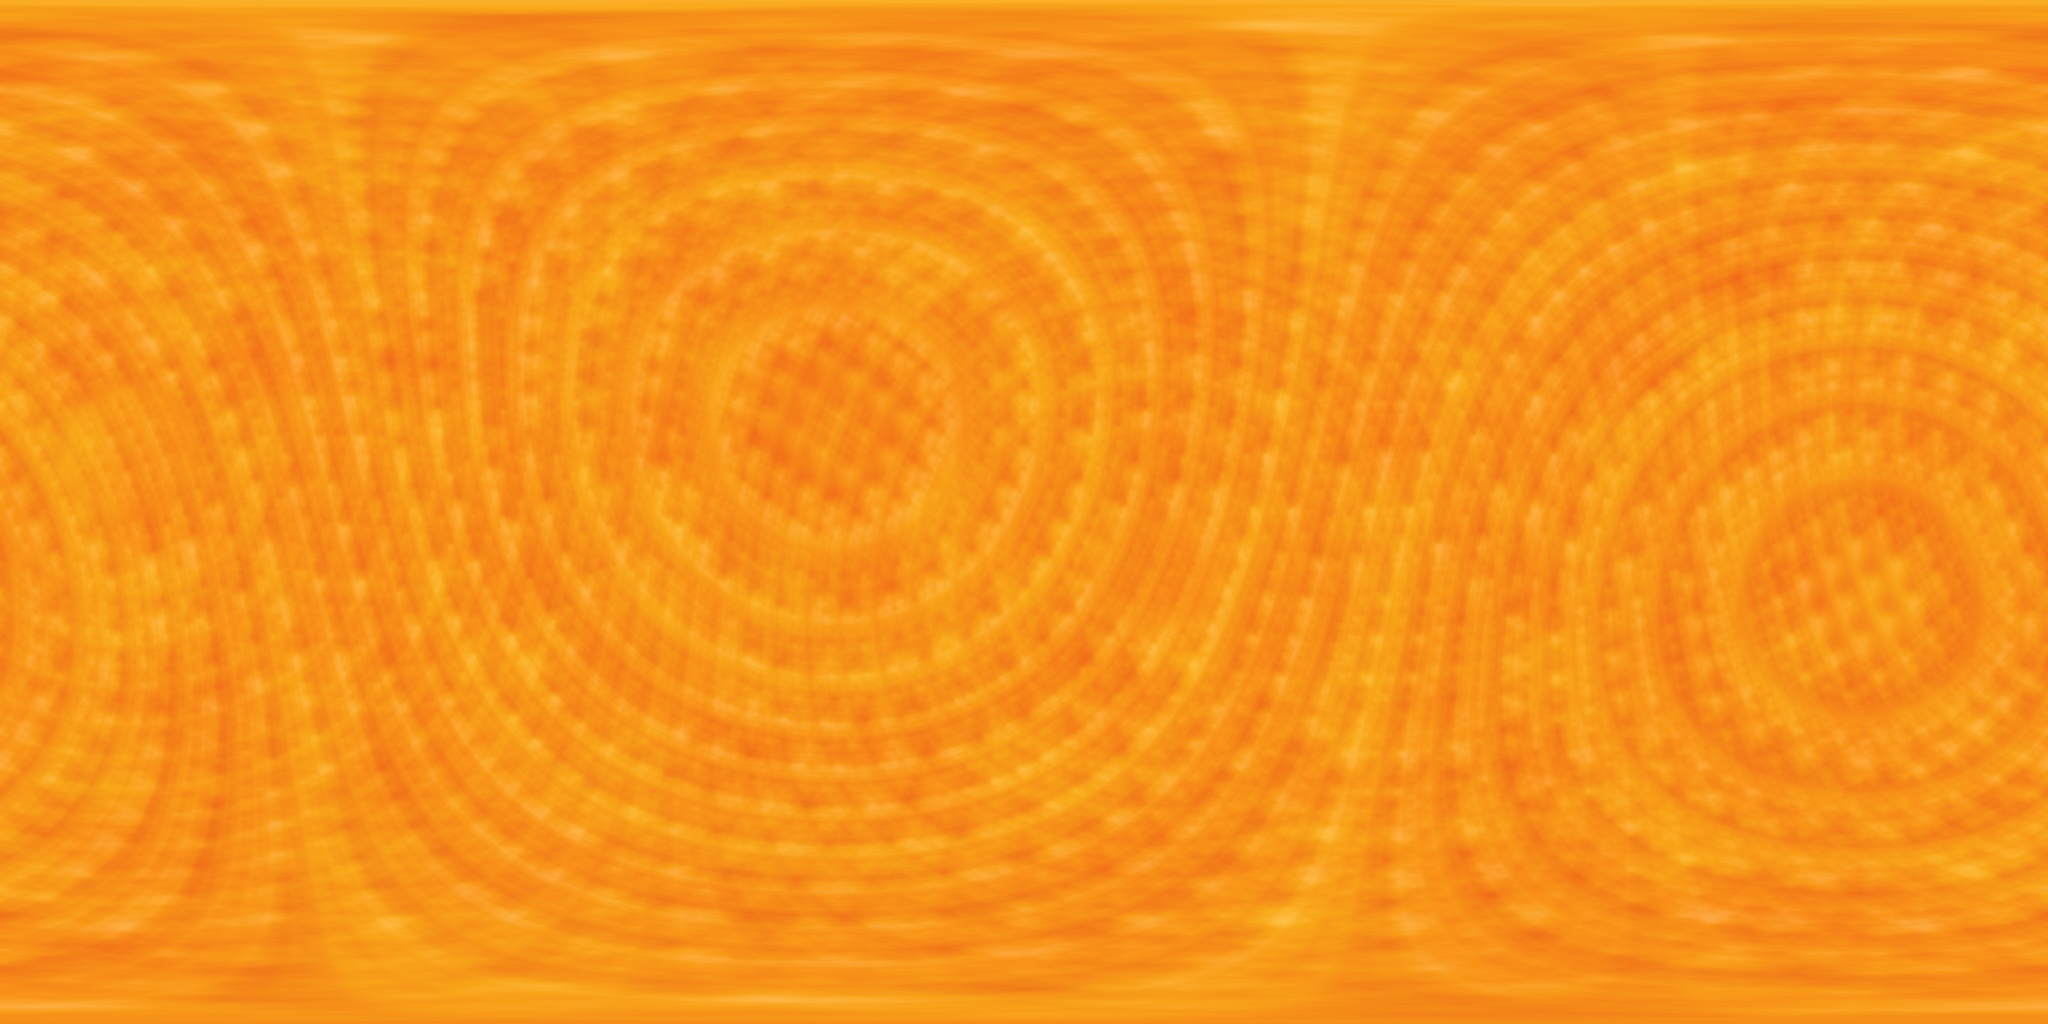
\includegraphics[width=\linewidth,height=4.4cm,keepaspectratio]{../public/textures/hd/sun_albedo.jpg}\\[2pt]
{\scriptsize\itshape\color{orbitarMuted} Planiglob desfășurat: Harta fotosferei solare în rezoluție 2K folosită în Orbitar (date NASA Solar Dynamics Observatory, SDO).}
\end{tabular}
\end{center}


\begin{tcolorbox}[orbitardata, title={\textbf{Repere esențiale: Soarele}}]
\small
\begin{itemize}[leftmargin=1.4em, itemsep=2pt, topsep=2pt]
  \item \textbf{Clasificare și orbită:} Stea \quad$\bullet$\quad \textbf{Distanță:} 0 UA (Centrul Sistemului Solar)
  \item \textbf{Dimensiuni și masă:} rază medie 696.340 de kilometri \quad$\bullet$\quad masă: 332946,000 $\times M_\oplus$
  \item \textbf{Gravitație și regim termic:} 27,940 $\times g_\oplus$ (274,09 m/s$^2$) \quad$\bullet$\quad temperatură medie: +5.505 $^\circ$C (înclinarea axei: 7,25$^\circ$)
  \item \textbf{Ciclu orbital și rotație:} perioadă orbitală (an): Orbitează centrul Căii Lactee (aproximativ 230 de milioane de ani) \quad$\bullet$\quad rotație (zi): 609,12 ore (25,38 zile pământești)
  \item \textbf{Durata călătoriei de pe Pământ:} cu viteza luminii ($1c$): \emph{8 minute și 20 de secunde}; cu racheta ($50.000$ de kilometri pe oră): \emph{4 luni cu o navă spațială rapidă}; cu avionul ($900$ de kilometri pe oră): \emph{19 ani cu un avion de pasageri}; cu mașina ($100$ de kilometri pe oră): \emph{171 de ani (fără oprire, cu 100 kilometri pe oră)}.
  \item \textbf{Repere de scară și curiozitate:} Dacă Soarele ar fi cât o minge mare de plajă, Pământul ar fi doar cât un bob mic de mazăre! În interiorul Soarelui ar încăpea aproximativ 1,3 milioane de planete Pământ!
\end{itemize}
\end{tcolorbox}

\subsubsection*{Prezentare generală și profil astrofizic}
Soarele este o stea de tip spectral G2V care concentrează 99,86\% din masa totală a Sistemului Solar. În nucleul său, la temperaturi de 15 milioane $^\circ$C, fuziunea nucleară transformă 600 de milioane de tone de hidrogen în heliu în fiecare secundă. Soarele este o minge uriașă de foc și plasmă strălucitoare care ne dă lumină și căldură în fiecare zi. Fără el, pe Pământ ar fi întuneric și un frig de gheață! Dacă Soarele ar fi cât o minge mare de plajă, Pământul ar fi doar cât un bob mic de mazăre!

\subsubsection*{Alcătuirea fizică și structura internă}
Privind în profunzimea sa, alcătuirea fizică este organizată pe mai multe straturi și regiuni distincte, fiecare având un rol bine definit în evoluția și dinamica acestui obiect cosmic. În primul rând se remarcă \textbf{Nucleul solar}, zona centrală extrem de densă (15.000.000 $^\circ$C) unde au loc reacțiile de fuziune proton-proton. În strânsă legătură cu această componentă se află \textbf{Zona radiativă și convectivă}, straturile prin care fotonii și curenții de plasmă transportă energia spre suprafață timp de mii de ani. În completarea acestui ansamblu întâlnim \textbf{Fotosfera și Coroana}, suprafața vizibilă la 5.505 $^\circ$C și atmosfera exterioară rarefiată care depășește 1.000.000 $^\circ$C.

\subsubsection*{Observații astronomice și istoricul explorării}
Studiat de misiunile SOHO, Solar Dynamics Observatory (SDO), Solar Orbiter (ESA) și Parker Solar Probe (NASA), care a pătruns direct în coroana solară. În interiorul Soarelui ar încăpea aproximativ 1,3 milioane de planete Pământ!

\vspace{6pt}
\begin{tcolorbox}[orbitarquiz, title={\textbf{Întrebare de verificare \#1: Soarele}}]
\textbf{Ce procent din masa întregului Sistem Solar se află în Soare?}
\begin{itemize}[leftmargin=2.2em, itemsep=2pt, topsep=4pt]
  \item[$\square$ \textbf{A.}] Aproximativ 50\%
  \item[$\square$ \textbf{B.}] Aproximativ 75\%
  \item[$\square$ \textbf{C.}] Peste 99,8\%
  \item[$\square$ \textbf{D.}] Sub 25\%
\end{itemize}
\vspace{2pt}
{\footnotesize\color{orbitarMuted}\textbf{Răspuns corect:} \textbf{C} (Peste 99,8\%). \emph{Soarele concentrează 99,86\% din masa Sistemului Solar; toate planetele, lunile și asteroizii la un loc reprezintă doar 0,14\%!}}
\end{tcolorbox}
\clearpage


\section{Mercur}
\label{sec:body-mercury}
\vspace{-4pt}
{\large\itshape\color{orbitarAccent} Cea mai apropiată și mai mică planetă de la Soare}\\[4pt]


\begin{center}
\begin{tabular}{@{}m{0.44\textwidth}@{\hspace{0.03\textwidth}}m{0.51\textwidth}@{}}
\centering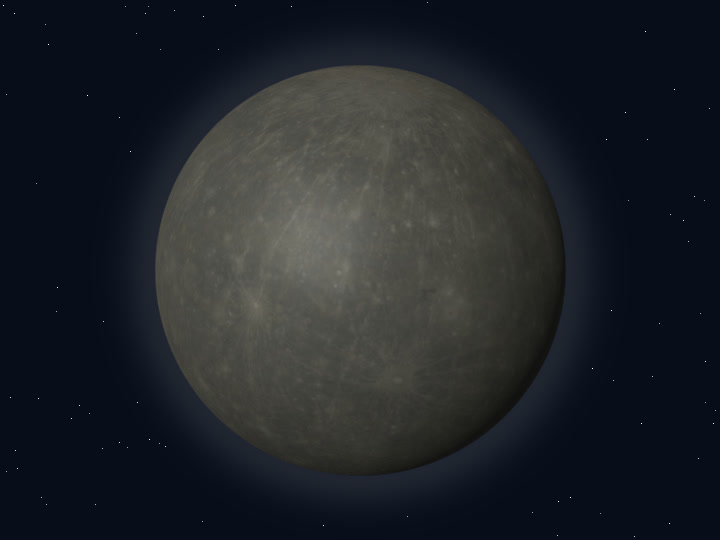
\includegraphics[width=\linewidth,height=4.4cm,keepaspectratio]{imagini/globuri/mercury.jpg}\\[2pt]
{\scriptsize\itshape\color{orbitarMuted} Vedere 3D a corpului ceresc (\textbf{Mercur})}
&
\centering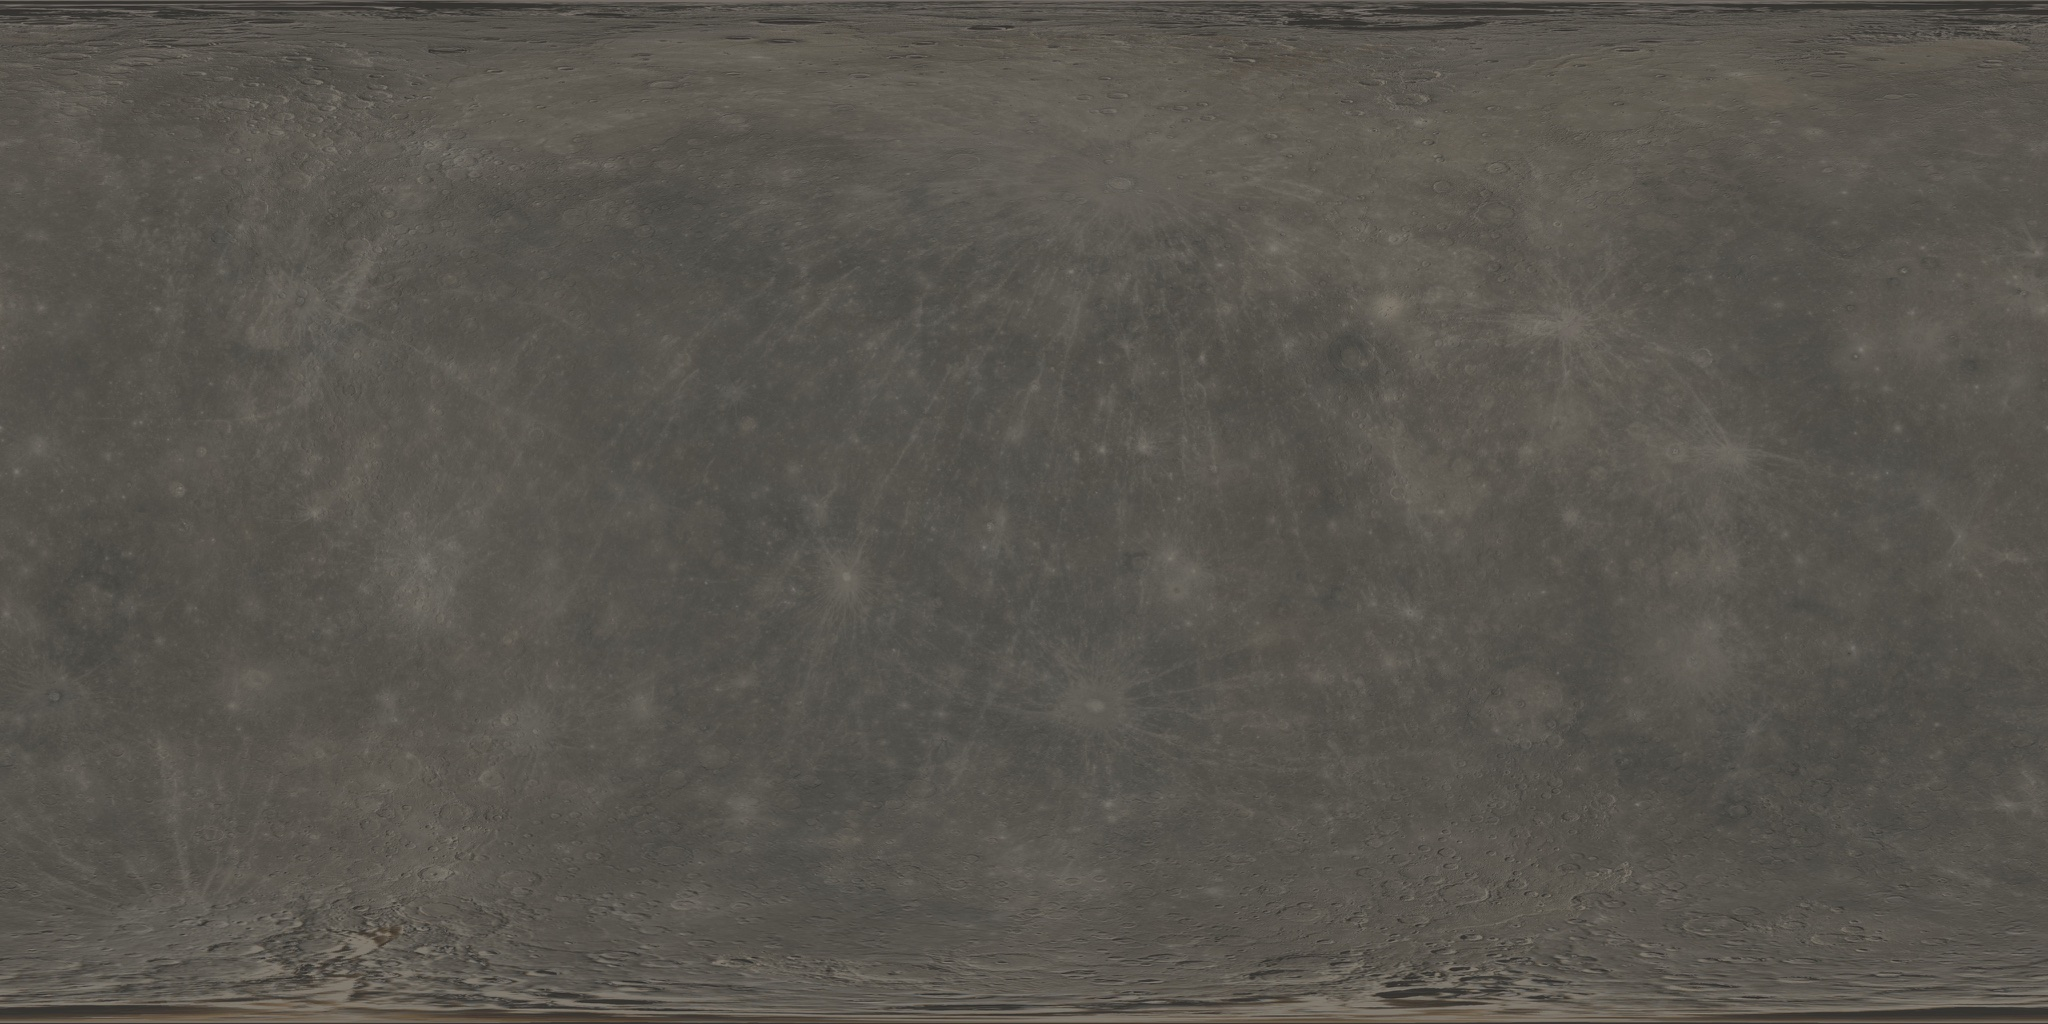
\includegraphics[width=\linewidth,height=4.4cm,keepaspectratio]{../public/textures/hd/mercury_messenger_albedo.jpg}\\[2pt]
{\scriptsize\itshape\color{orbitarMuted} Planiglob desfășurat: Harta globală a suprafeței craterizate a lui Mercur, realizată de sonda NASA MESSENGER (2K HD).}
\end{tabular}
\end{center}


\begin{tcolorbox}[orbitardata, title={\textbf{Repere esențiale: Mercur}}]
\small
\begin{itemize}[leftmargin=1.4em, itemsep=2pt, topsep=2pt]
  \item \textbf{Clasificare și orbită:} Planetă Telurică (Stâncoasă) \quad$\bullet$\quad \textbf{Distanță:} 0,387 UA ($\approx$ 58 milioane de kilometri)
  \item \textbf{Dimensiuni și masă:} rază medie 2.439,7 de kilometri \quad$\bullet$\quad masă: 0,055 $\times M_\oplus$
  \item \textbf{Gravitație și regim termic:} 0,380 $\times g_\oplus$ (3,73 m/s$^2$) \quad$\bullet$\quad temperatură medie: +167 $^\circ$C (înclinarea axei: 0,03$^\circ$)
  \item \textbf{Ciclu orbital și rotație:} perioadă orbitală (an): 87,97 zile pământești \quad$\bullet$\quad rotație (zi): 1407,60 ore (58,65 zile pământești)
  \item \textbf{Durata călătoriei de pe Pământ:} cu viteza luminii ($1c$): \emph{5 minute de pe Pământ}; cu racheta ($50.000$ de kilometri pe oră): \emph{3 luni}; cu avionul ($900$ de kilometri pe oră): \emph{11 ani și jumătate}; cu mașina ($100$ de kilometri pe oră): \emph{105 ani}.
  \item \textbf{Repere de scară și curiozitate:} Mercur este doar puțin mai mare decât Luna noastră și arată aproape ca o nucă cenușie plină de gropițe. Deși este cel mai aproape de Soare, noaptea pe Mercur îngheață totul la -180 $^\circ$C pentru că nu are o pătură de aer!
\end{itemize}
\end{tcolorbox}

\subsubsection*{Prezentare generală și profil astrofizic}
Mercur este o planetă telurică densă, având un nucleu metalic uriaș din fier care ocupă 85\% din raza planetei. Lipsa unei atmosfere substanțiale (are doar o exosferă subțire) provoacă cele mai mari variații termice din Sistemul Solar. Mercur este mesagerul rapid al Sistemului Solar! Fiind cel mai aproape de Soare, termină o tură completă în doar 88 de zile. Mercur este doar puțin mai mare decât Luna noastră și arată aproape ca o nucă cenușie plină de gropițe.

\subsubsection*{Alcătuirea fizică și structura internă}
Privind în profunzimea sa, alcătuirea fizică este organizată pe mai multe straturi și regiuni distincte, fiecare având un rol bine definit în evoluția și dinamica acestui obiect cosmic. În primul rând se remarcă \textbf{Nucleu metalic supradimensionat}, format din fier solid și lichid, reprezintă aproximativ 85\% din raza planetei și generează un câmp magnetic propriu. În strânsă legătură cu această componentă se află \textbf{Manta silicatată subțire}, un înveliș de roci de numai 400 de kilometri grosime. În completarea acestui ansamblu întâlnim \textbf{Scoarță craterizată}, dominată de Bazinul Caloris (1.550 de kilometri diametru) și faleze de contracție numite rupes.

\subsubsection*{Observații astronomice și istoricul explorării}
Vizitată de Mariner 10 (1974--1975), cartografiată complet de sonda MESSENGER (2011--2015) și explorată de misiunea europeo-japoneză BepiColombo. Deși este cel mai aproape de Soare, noaptea pe Mercur îngheață totul la -180 $^\circ$C pentru că nu are o pătură de aer!

\vspace{6pt}
\begin{tcolorbox}[orbitarquiz, title={\textbf{Întrebare de verificare \#2: Mercur}}]
\textbf{Cât durează un an pe planeta Mercur (o orbită completă în jurul Soarelui)?}
\begin{itemize}[leftmargin=2.2em, itemsep=2pt, topsep=4pt]
  \item[$\square$ \textbf{A.}] 365 de zile
  \item[$\square$ \textbf{B.}] 88 de zile pământești
  \item[$\square$ \textbf{C.}] 24 de ore
  \item[$\square$ \textbf{D.}] 12 ani
\end{itemize}
\vspace{2pt}
{\footnotesize\color{orbitarMuted}\textbf{Răspuns corect:} \textbf{B} (88 de zile pământești). \emph{Fiind cea mai apropiată planetă de Soare, Mercur parcurge orbita cu aproximativ 47 kilometri pe secundă și încheie un an în doar 88 de zile terestre.}}
\end{tcolorbox}
\clearpage


\section{Venus}
\label{sec:body-venus}
\vspace{-4pt}
{\large\itshape\color{orbitarAccent} Luceafărul strălucitor cu efect de seră extrem}\\[4pt]


\begin{center}
\begin{tabular}{@{}m{0.44\textwidth}@{\hspace{0.03\textwidth}}m{0.51\textwidth}@{}}
\centering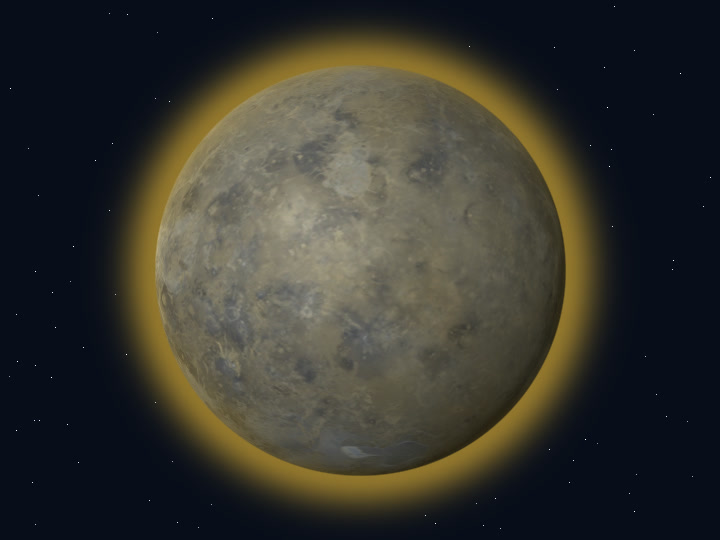
\includegraphics[width=\linewidth,height=4.4cm,keepaspectratio]{imagini/globuri/venus.jpg}\\[2pt]
{\scriptsize\itshape\color{orbitarMuted} Vedere 3D a corpului ceresc (\textbf{Venus})}
&
\centering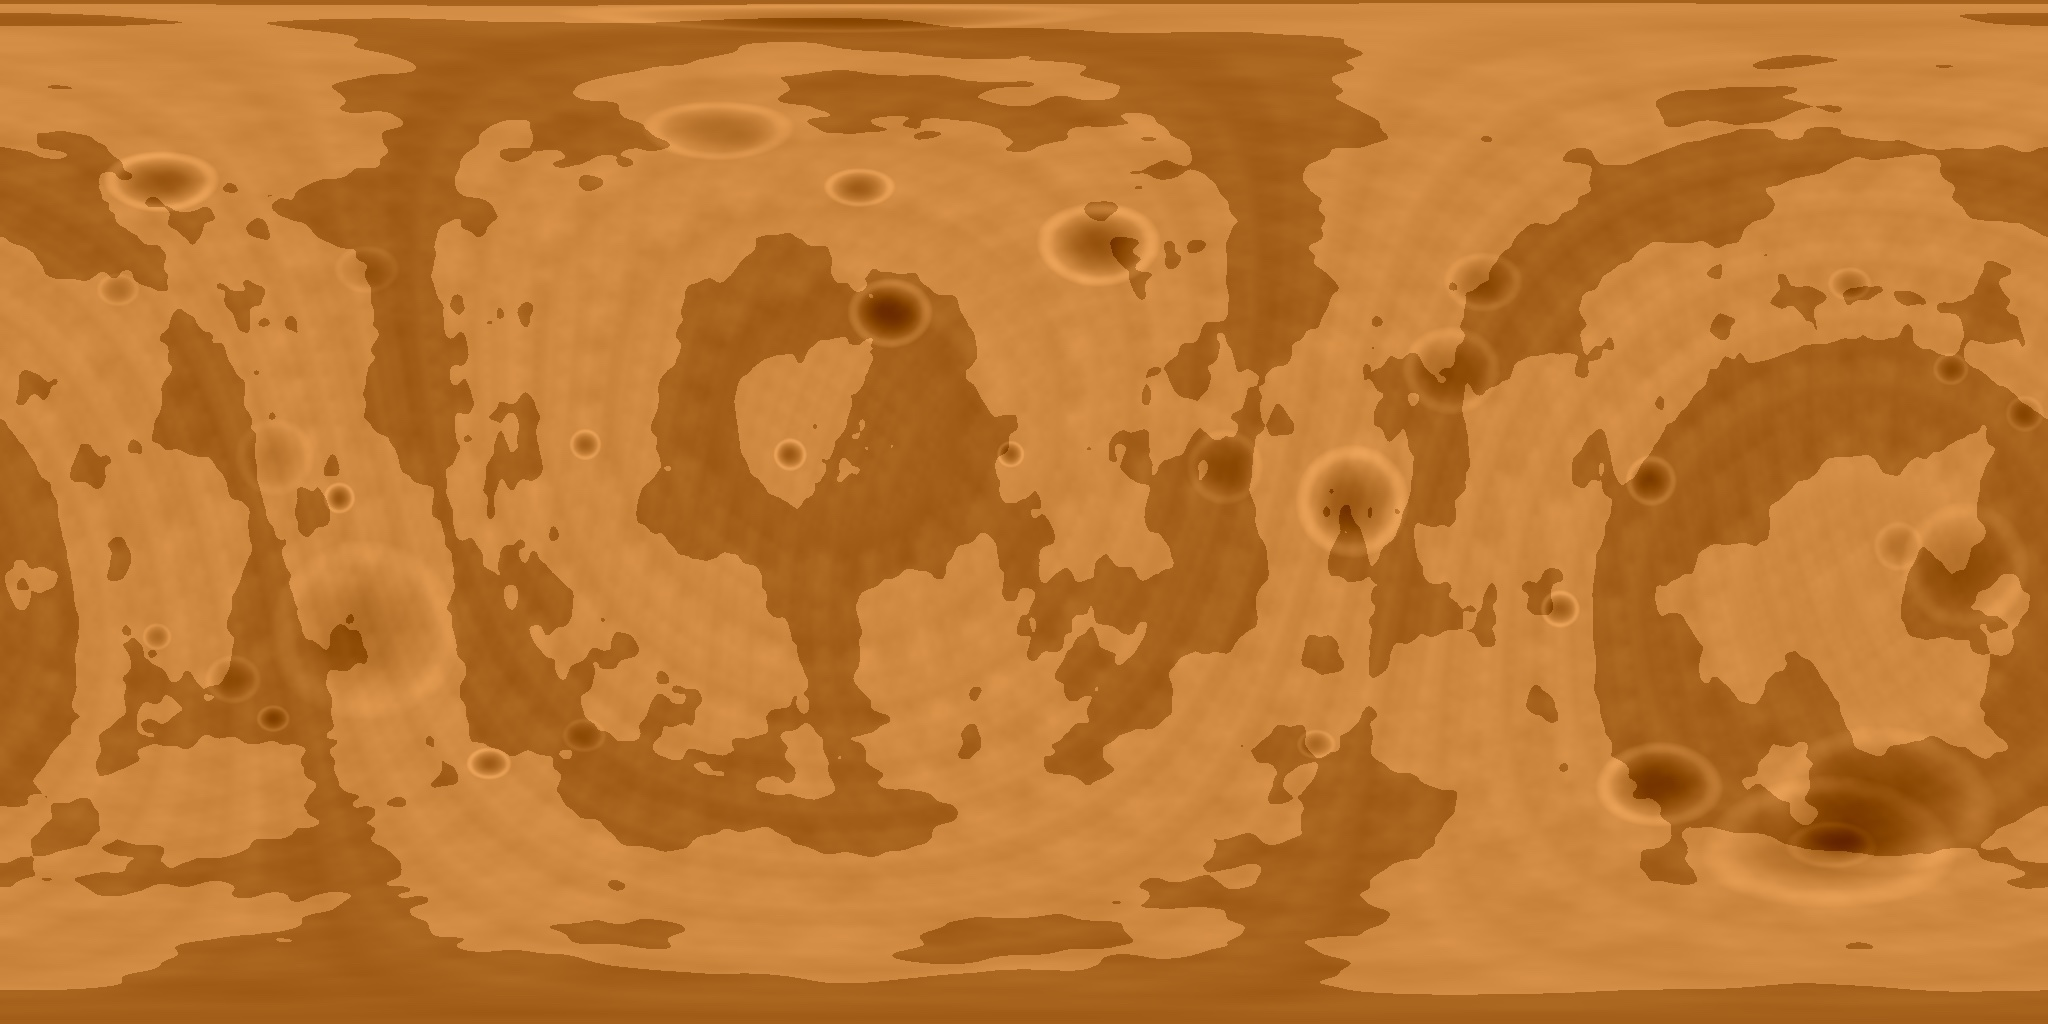
\includegraphics[width=\linewidth,height=4.4cm,keepaspectratio]{../public/textures/hd/venus_magellan_surface.jpg}\\[2pt]
{\scriptsize\itshape\color{orbitarMuted} Planiglob desfășurat: Harta radar a reliefului vulcanic de sub norii planetei Venus, obținută de sonda NASA Magellan (modul \quotedblbase{}Vezi sub nori\textquotedblright{} în Orbitar).}
\end{tabular}
\end{center}


\begin{tcolorbox}[orbitardata, title={\textbf{Repere esențiale: Venus}}]
\small
\begin{itemize}[leftmargin=1.4em, itemsep=2pt, topsep=2pt]
  \item \textbf{Clasificare și orbită:} Planetă Telurică (Stâncoasă) \quad$\bullet$\quad \textbf{Distanță:} 0,723 UA ($\approx$ 108 milioane de kilometri)
  \item \textbf{Dimensiuni și masă:} rază medie 6.051,8 de kilometri \quad$\bullet$\quad masă: 0,815 $\times M_\oplus$
  \item \textbf{Gravitație și regim termic:} 0,900 $\times g_\oplus$ (8,83 m/s$^2$) \quad$\bullet$\quad temperatură medie: +464 $^\circ$C (înclinarea axei: 177,36$^\circ$)
  \item \textbf{Ciclu orbital și rotație:} perioadă orbitală (an): 224,7 zile pământești \quad$\bullet$\quad rotație (zi): 5832,50 ore (Rotație retrogradă!)
  \item \textbf{Durata călătoriei de pe Pământ:} cu viteza luminii ($1c$): \emph{2 minute și 18 secunde}; cu racheta ($50.000$ de kilometri pe oră): \emph{3 luni și jumătate}; cu avionul ($900$ de kilometri pe oră): \emph{5 ani și 2 luni}; cu mașina ($100$ de kilometri pe oră): \emph{47 de ani (când este cel mai aproape)}.
  \item \textbf{Repere de scară și curiozitate:} Venus are aproape aceeași mărime ca Pământul, asemenea a două portocale așezate una lângă alta! Pe Venus, Soarele răsare din vest și apune în est, deoarece planeta se învârte invers față de Pământ!
\end{itemize}
\end{tcolorbox}

\subsubsection*{Prezentare generală și profil astrofizic}
Numită sora geamănă a Pământului datorită dimensiunii și masei similare, Venus are o atmosferă compusă în proporție de 96,5\% din dioxid de carbon, cu o presiune la sol de 92 de ori mai mare decât cea terestră. Venus este cel mai strălucitor obiect de pe cerul nopții după Lună! Este învelită în nori groși și gălbui care păstrează căldura ca într-un cuptor. Venus are aproape aceeași mărime ca Pământul, asemenea a două portocale așezate una lângă alta!

\subsubsection*{Alcătuirea fizică și structura internă}
Privind în profunzimea sa, alcătuirea fizică este organizată pe mai multe straturi și regiuni distincte, fiecare având un rol bine definit în evoluția și dinamica acestui obiect cosmic. În primul rând se remarcă \textbf{Nucleu de fier și nichel}, similar cu cel terestru, dar fără efectul de dinam magnetic din cauza rotației extrem de lente. În strânsă legătură cu această componentă se află \textbf{Manta și scoarță vulcanică}, peste 1.600 de vulcani majori, platouri ca Ishtar Terra și munții Maxwell Montes. În completarea acestui ansamblu întâlnim \textbf{Atmosferă super-densă}, nori de acid sulfuric și CO$_2$ care mențin temperatura medie la +464 $^\circ$C.

\subsubsection*{Observații astronomice și istoricul explorării}
Sondele sovietice Venera au reușit primele asolizări și fotografii de pe suprafață (1970--1982), iar sonda NASA Magellan a cartografiat relieful prin radar. Pe Venus, Soarele răsare din vest și apune în est, deoarece planeta se învârte invers față de Pământ!

\vspace{6pt}
\begin{tcolorbox}[orbitarquiz, title={\textbf{Întrebare de verificare \#3: Venus}}]
\textbf{De ce este Venus mai fierbinte decât Mercur, deși se află mai departe de Soare?}
\begin{itemize}[leftmargin=2.2em, itemsep=2pt, topsep=4pt]
  \item[$\square$ \textbf{A.}] Are mai mulți vulcani activi
  \item[$\square$ \textbf{B.}] Are o atmosferă densă de CO$_2$ care creează un efect de seră extrem
  \item[$\square$ \textbf{C.}] Este mai mare decât Mercur
  \item[$\square$ \textbf{D.}] Se rotește foarte repede
\end{itemize}
\vspace{2pt}
{\footnotesize\color{orbitarMuted}\textbf{Răspuns corect:} \textbf{B} (Are o atmosferă densă de CO$_2$ care creează un efect de seră extrem). \emph{Atmosfera groasă de dioxid de carbon captează radiația termică, ridicând temperatura la +464 $^\circ$C pe toată suprafața planetei.}}
\end{tcolorbox}
\clearpage


\section{Pământul}
\label{sec:body-earth}
\vspace{-4pt}
{\large\itshape\color{orbitarAccent} Planeta Albastră, singura lume cunoscută care găzduiește viață}\\[4pt]


\begin{center}
\begin{tabular}{@{}m{0.44\textwidth}@{\hspace{0.03\textwidth}}m{0.51\textwidth}@{}}
\centering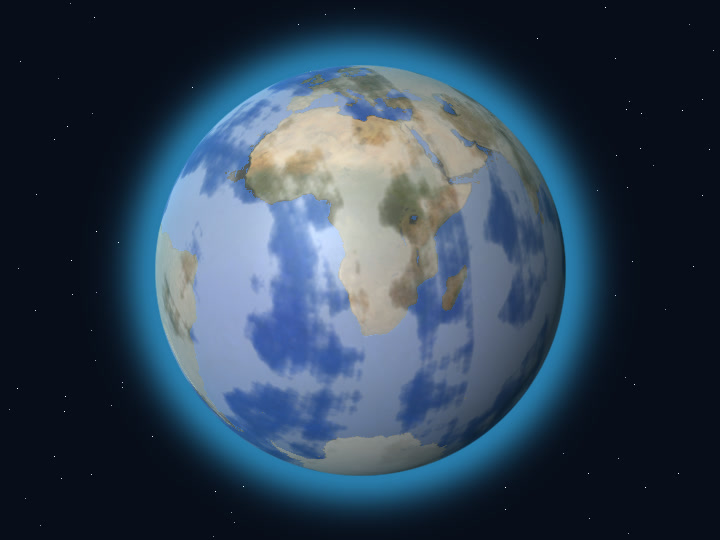
\includegraphics[width=\linewidth,height=4.4cm,keepaspectratio]{imagini/globuri/earth.jpg}\\[2pt]
{\scriptsize\itshape\color{orbitarMuted} Vedere 3D a corpului ceresc (\textbf{Pământul})}
&
\centering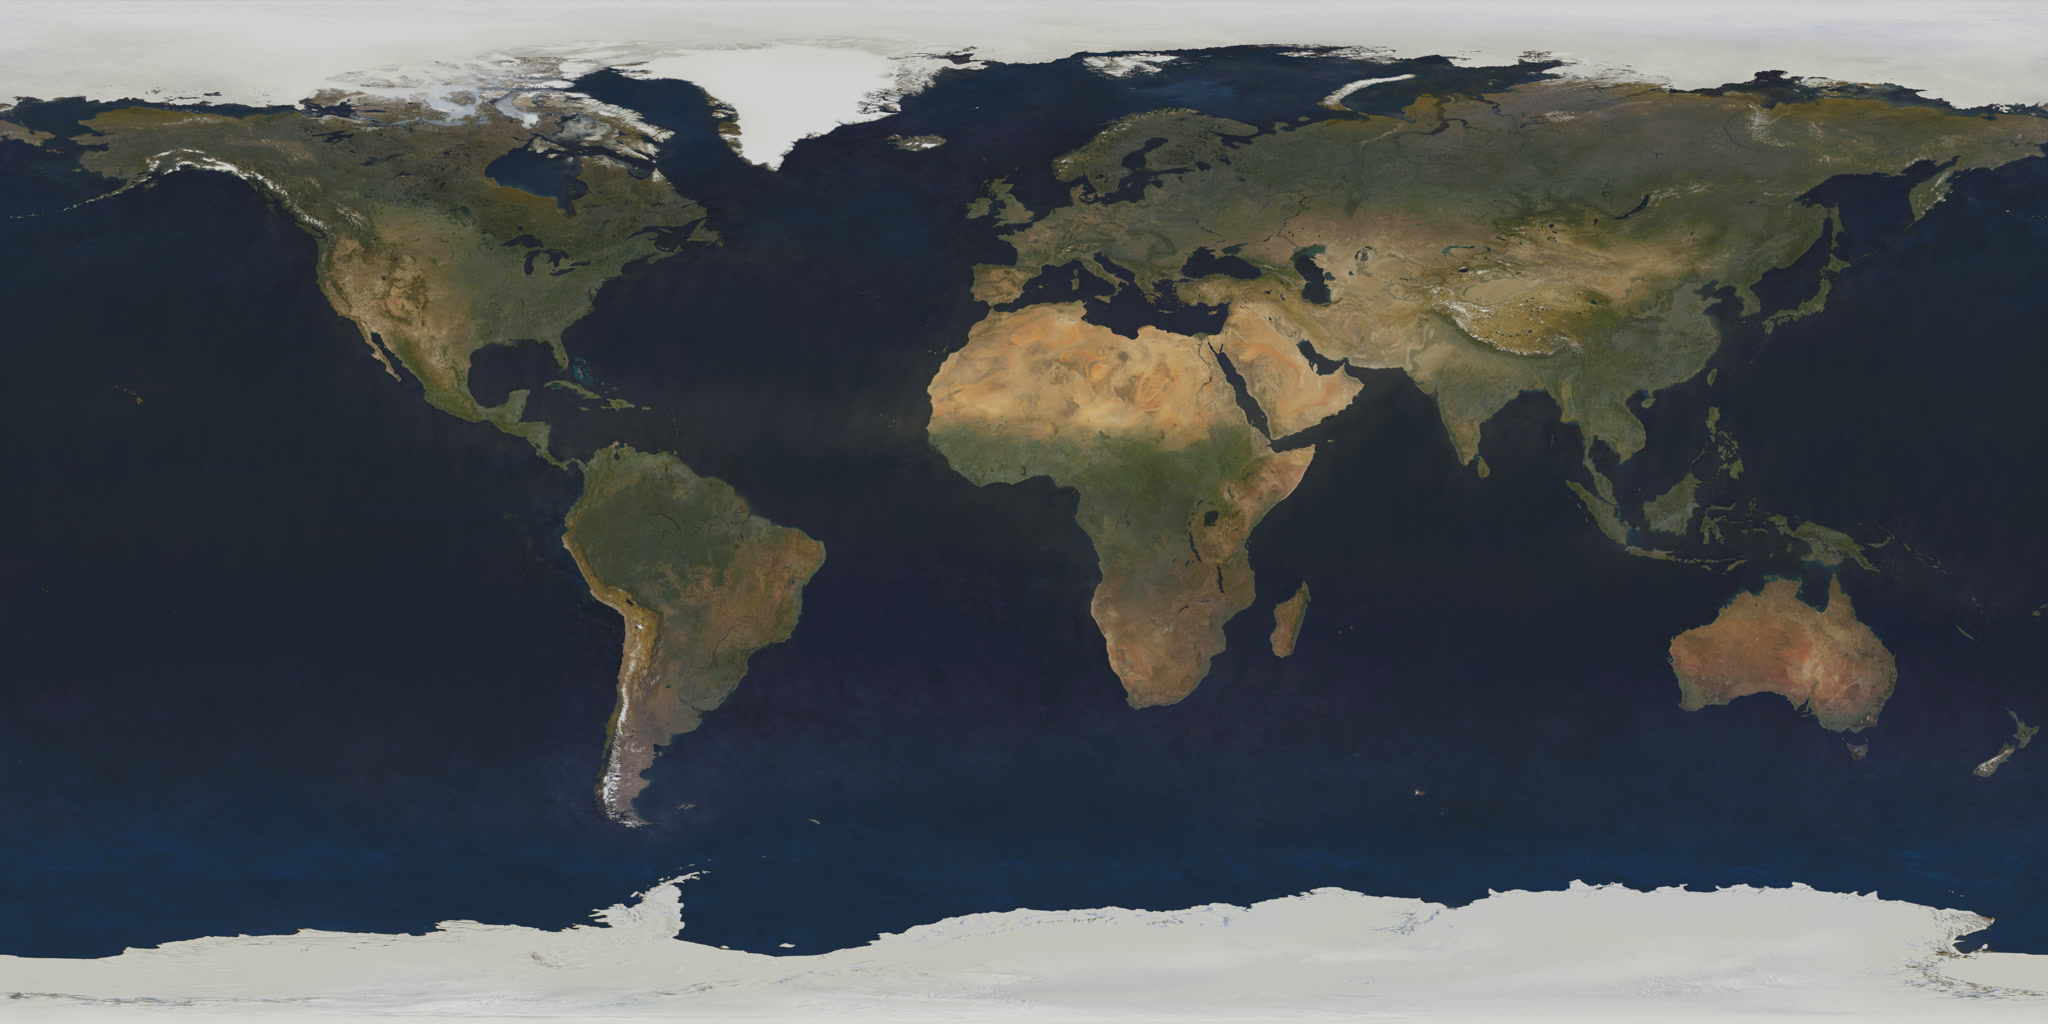
\includegraphics[width=\linewidth,height=4.4cm,keepaspectratio]{../public/textures/hd/earth_albedo.jpg}\\[2pt]
{\scriptsize\itshape\color{orbitarMuted} Planiglob desfășurat: Harta globală NASA Blue Marble a planetei Pământ, cu oceanele, continentele și calotele polare.}
\end{tabular}
\end{center}


\begin{tcolorbox}[orbitardata, title={\textbf{Repere esențiale: Pământul}}]
\small
\begin{itemize}[leftmargin=1.4em, itemsep=2pt, topsep=2pt]
  \item \textbf{Clasificare și orbită:} Planetă Telurică (Stâncoasă) \quad$\bullet$\quad \textbf{Distanță:} 1,000 UA ($\approx$ 150 milioane de kilometri)
  \item \textbf{Dimensiuni și masă:} rază medie 6.371 de kilometri \quad$\bullet$\quad masă: 1,000 $\times M_\oplus$
  \item \textbf{Gravitație și regim termic:} 1,000 $\times g_\oplus$ (9,81 m/s$^2$) \quad$\bullet$\quad temperatură medie: +15 $^\circ$C (înclinarea axei: 23,44$^\circ$)
  \item \textbf{Ciclu orbital și rotație:} perioadă orbitală (an): 365,256 zile ($\approx$ 1,00 ani pământești) \quad$\bullet$\quad rotație (zi): 23,93 ore (1,00 zile pământești)
  \item \textbf{Durata călătoriei de pe Pământ:} cu viteza luminii ($1c$): \emph{0,13 secunde în jurul Ecuatorului}; cu racheta ($50.000$ de kilometri pe oră): \emph{90 de minute pentru o orbită completă}; cu avionul ($900$ de kilometri pe oră): \emph{45 de ore în jurul lumii}; cu mașina ($100$ de kilometri pe oră): \emph{Ești deja aici! Înconjurul Ecuatorului durează 17 zile cu mașina}.
  \item \textbf{Repere de scară și curiozitate:} Văzut din spațiu, Pământul seamănă cu o bilă de sticlă albastră cu vârtejuri albe de frișcă! Pământul nu este perfect rotund: pentru că se învârte, este puțin turtit la poli ca o mandarină!
\end{itemize}
\end{tcolorbox}

\subsubsection*{Prezentare generală și profil astrofizic}
A treia planetă de la Soare definește distanța etalon de 1 Unitate Astronomică (149.597.870 de kilometri). Este singurul corp planetar cu tectonică a plăcilor activă, hidrosferă lichidă (71\% din suprafață) și atmosferă bogată în azot (78\%) și oxigen (21\%). Pământul este casa noastră minunată din cosmos! Are oceane albastre, continente verzi, nori albi și o pătură de aer respirabil care ne apără. Văzut din spațiu, Pământul seamănă cu o bilă de sticlă albastră cu vârtejuri albe de frișcă!

\subsubsection*{Alcătuirea fizică și structura internă}
Privind în profunzimea sa, alcătuirea fizică este organizată pe mai multe straturi și regiuni distincte, fiecare având un rol bine definit în evoluția și dinamica acestui obiect cosmic. În primul rând se remarcă \textbf{Nucleu intern solid și extern lichid}, aliaj de fier-nichel care generează magnetosfera protectoare împotriva radiațiilor cosmice. În strânsă legătură cu această componentă se află \textbf{Manta silicatată și Litosferă}, unde curenții de convecție din manta pun în mișcare plăcile tectonice ale scoarței. În completarea acestui ansamblu întâlnim \textbf{Hidrosferă și Atmosferă}, unde oceanele și straturile atmosferice (troposferă, stratosferă cu stratul de ozon) reglează clima.

\subsubsection*{Observații astronomice și istoricul explorării}
Observată continuu de flote de sateliți meteorologici și științifici (programul european Copernicus Sentinel, NASA EOS) și de echipajele de pe ISS. Pământul nu este perfect rotund: pentru că se învârte, este puțin turtit la poli ca o mandarină!

\vspace{6pt}
\begin{tcolorbox}[orbitarquiz, title={\textbf{Întrebare de verificare \#4: Pământul}}]
\textbf{Ce ne protejează planeta de particulele încărcate electric ale vântului solar?}
\begin{itemize}[leftmargin=2.2em, itemsep=2pt, topsep=4pt]
  \item[$\square$ \textbf{A.}] Câmpul magnetic (magnetosfera) generat de nucleul Pământului
  \item[$\square$ \textbf{B.}] Gravitația Lunii
  \item[$\square$ \textbf{C.}] Rotația în jurul Soarelui
  \item[$\square$ \textbf{D.}] Norii din troposferă
\end{itemize}
\vspace{2pt}
{\footnotesize\color{orbitarMuted}\textbf{Răspuns corect:} \textbf{A} (Câmpul magnetic (magnetosfera) generat de nucleul Pământului). \emph{Nucleul extern din fier lichid al Pământului funcționează ca un dinam și creează magnetosfera, care deviază vântul solar.}}
\end{tcolorbox}
\clearpage


\subsection{Luna}
\label{sec:body-moon}
\vspace{-4pt}
{\large\itshape\color{orbitarAccent} Singurul satelit natural al Pământului}\\[4pt]


\begin{center}
\begin{tabular}{@{}m{0.44\textwidth}@{\hspace{0.03\textwidth}}m{0.51\textwidth}@{}}
\centering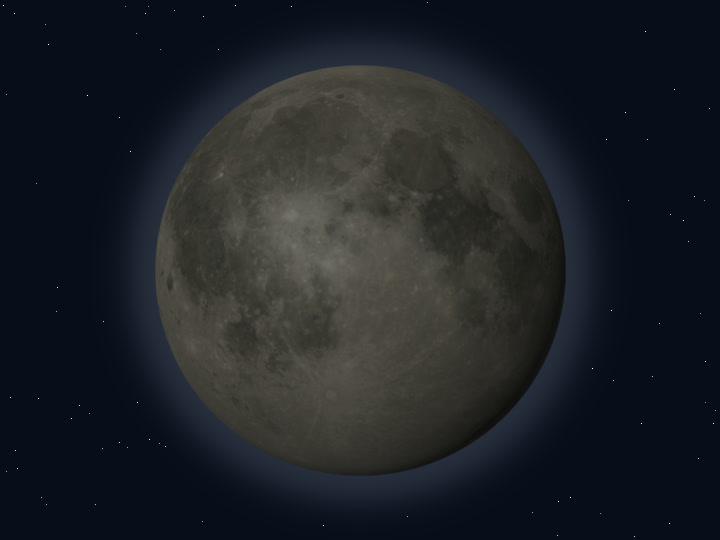
\includegraphics[width=\linewidth,height=4.4cm,keepaspectratio]{imagini/globuri/moon.jpg}\\[2pt]
{\scriptsize\itshape\color{orbitarMuted} Vedere 3D a corpului ceresc (\textbf{Luna})}
&
\centering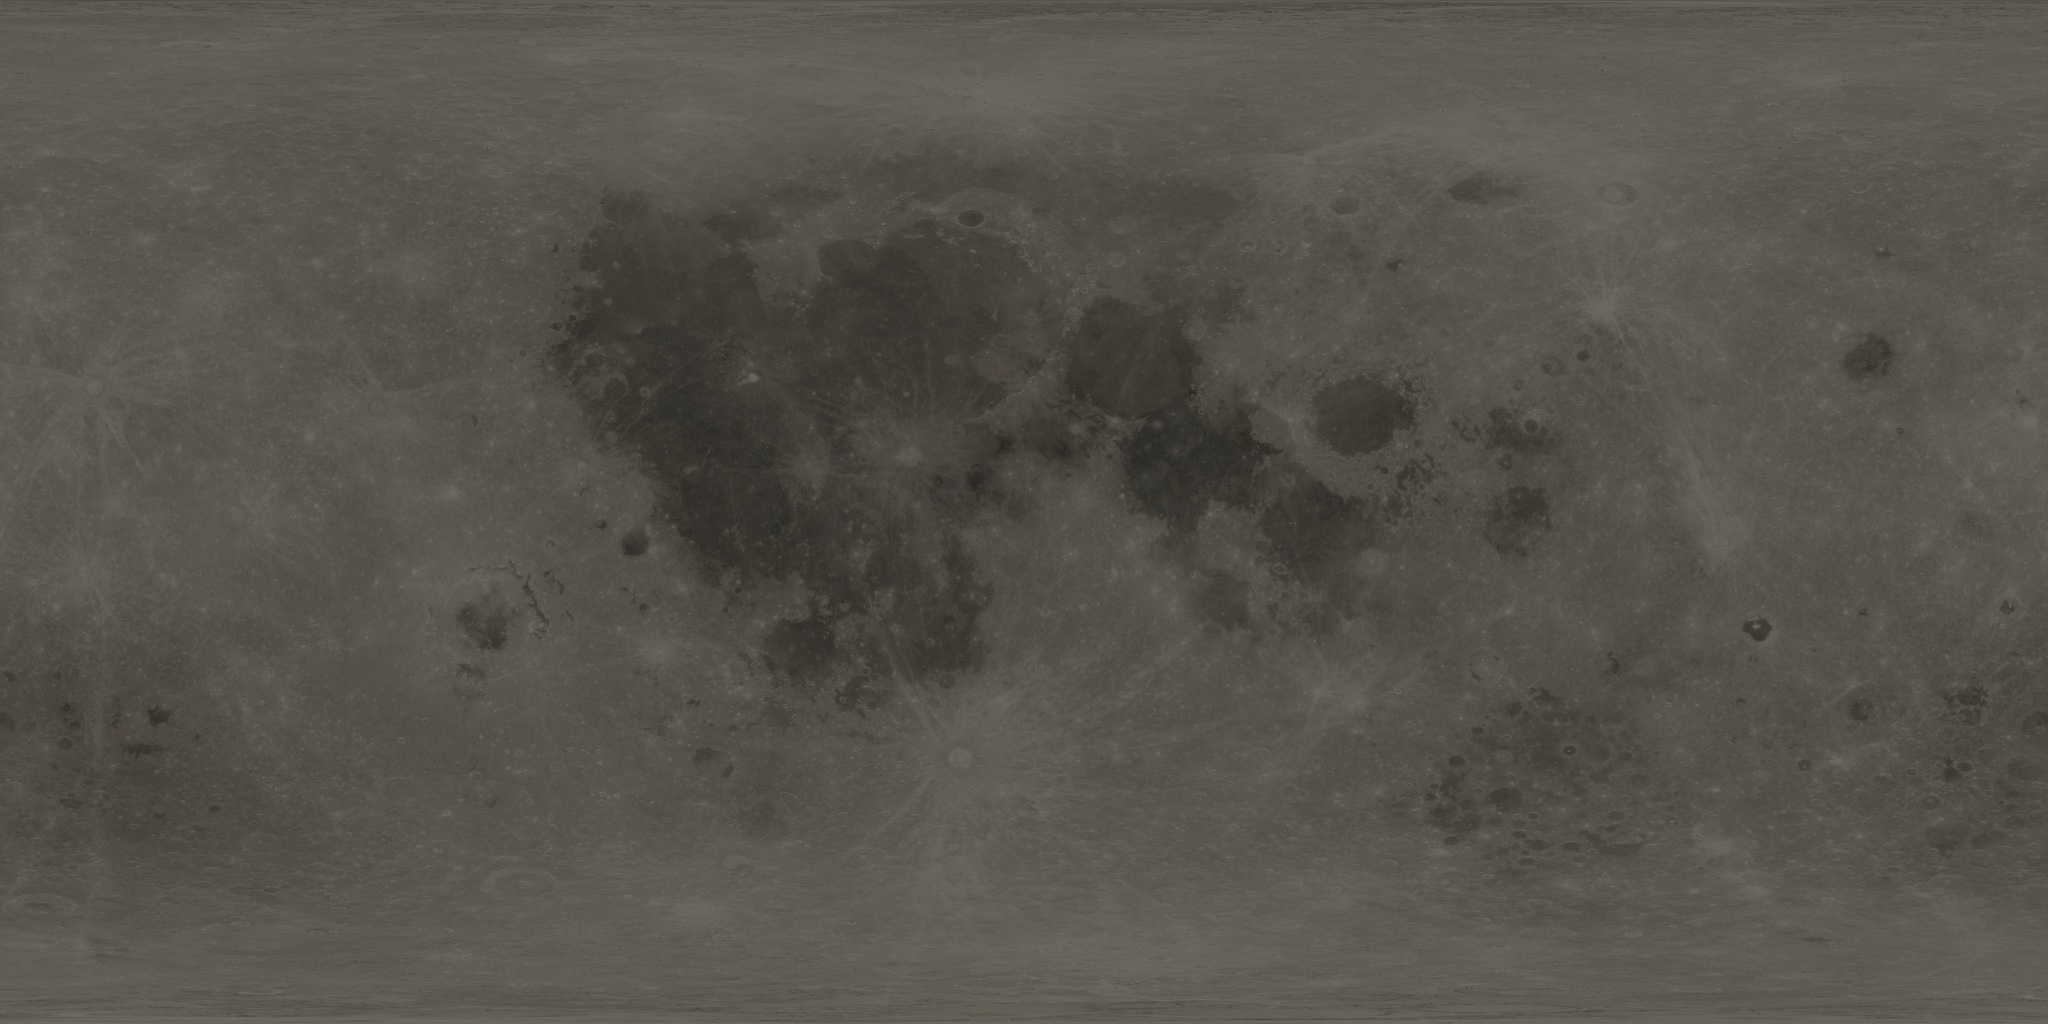
\includegraphics[width=\linewidth,height=4.4cm,keepaspectratio]{../public/textures/hd/moon_lro_albedo.jpg}\\[2pt]
{\scriptsize\itshape\color{orbitarMuted} Planiglob desfășurat: Harta globală a Lunii (NASA Lunar Reconnaissance Orbiter, LRO), cu mările bazaltice și craterele de impact.}
\end{tabular}
\end{center}


\begin{tcolorbox}[orbitardata, title={\textbf{Repere esențiale: Luna}}]
\small
\begin{itemize}[leftmargin=1.4em, itemsep=2pt, topsep=2pt]
  \item \textbf{Clasificare și orbită:} Satelit Natural (Lună) (orbitează în jurul: \textbf{Pământul}) \quad$\bullet$\quad \textbf{Distanță:} 1,000 UA ($\approx$ 150 milioane de kilometri)
  \item \textbf{Dimensiuni și masă:} rază medie 1.737,4 de kilometri \quad$\bullet$\quad masă: 0,012 $\times M_\oplus$
  \item \textbf{Gravitație și regim termic:} 0,165 $\times g_\oplus$ (1,62 m/s$^2$) \quad$\bullet$\quad temperatură medie: -23 $^\circ$C (înclinarea axei: 6,68$^\circ$)
  \item \textbf{Ciclu orbital și rotație:} perioadă orbitală (an): 27,322 zile pământești \quad$\bullet$\quad rotație (zi): 655,70 ore (27,32 zile pământești)
  \item \textbf{Durata călătoriei de pe Pământ:} cu viteza luminii ($1c$): \emph{1,28 secunde}; cu racheta ($50.000$ de kilometri pe oră): \emph{3 zile (misiunile Apollo)}; cu avionul ($900$ de kilometri pe oră): \emph{18 zile}; cu mașina ($100$ de kilometri pe oră): \emph{160 de zile (aproximativ 5 luni)}.
  \item \textbf{Repere de scară și curiozitate:} Dacă Pământul ar fi o minge de baschet, Luna ar fi cât o minge de tenis aflată la 7 metri distanță! Pe Lună gravitația este de 6 ori mai slabă decât pe Pământ: acolo ai putea sări de 6 ori mai sus!
\end{itemize}
\end{tcolorbox}

\subsubsection*{Prezentare generală și profil astrofizic}
Formată acum aproximativ 4,5 miliarde de ani în urma impactului dintre proto-Pământ și un corp de mărimea lui Marte (Theia), Luna se află în rotație sincronă (ne arată mereu aceeași față) și stabilizează înclinarea axei terestre. Luna este tovarășa fidelă a Pământului! Ea nu are lumină proprie, ci strălucește pe cerul nopții pentru că reflectă lumina Soarelui ca o oglindă. Dacă Pământul ar fi o minge de baschet, Luna ar fi cât o minge de tenis aflată la 7 metri distanță!

\subsubsection*{Alcătuirea fizică și structura internă}
Privind în profunzimea sa, alcătuirea fizică este organizată pe mai multe straturi și regiuni distincte, fiecare având un rol bine definit în evoluția și dinamica acestui obiect cosmic. În primul rând se remarcă \textbf{Nucleu mic de fier}, cu o rază de numai aproximativ 350 de kilometri, parțial topit la exterior. În strânsă legătură cu această componentă se află \textbf{Manta litosferică}, bogată în olivină și piroxen, mult mai rigidă decât mantaua Pământului. În completarea acestui ansamblu întâlnim \textbf{Scoarță acoperită cu regolit}, mări lunare întunecate (bazalt vulcanic antic) și podișuri înalte intens craterizate.

\subsubsection*{Observații astronomice și istoricul explorării}
Singurul corp ceresc pe care au pășit oamenii (12 astronauți în programul Apollo, 1969--1972) și ținta programului actual Artemis. Pe Lună gravitația este de 6 ori mai slabă decât pe Pământ: acolo ai putea sări de 6 ori mai sus!

\vspace{6pt}
\begin{tcolorbox}[orbitarquiz, title={\textbf{Întrebare de verificare \#5: Luna}}]
\textbf{De ce vedem de pe Pământ întotdeauna aceeași față a Lunii?}
\begin{itemize}[leftmargin=2.2em, itemsep=2pt, topsep=4pt]
  \item[$\square$ \textbf{A.}] Pentru că Luna nu se rotește deloc
  \item[$\square$ \textbf{B.}] Pentru că perioada de rotație a Lunii este egală cu perioada ei de orbitare în jurul Pământului
  \item[$\square$ \textbf{C.}] Pentru că cealaltă față este mereu în întuneric
  \item[$\square$ \textbf{D.}] Din cauza norilor terestri
\end{itemize}
\vspace{2pt}
{\footnotesize\color{orbitarMuted}\textbf{Răspuns corect:} \textbf{B} (Pentru că perioada de rotație a Lunii este egală cu perioada ei de orbitare în jurul Pământului). \emph{Fenomenul se numește rotație sincronă: Luna se rotește în jurul axei sale în exact 27,3 zile, adică în același timp în care înconjoară Pământul.}}
\end{tcolorbox}
\vspace{6pt}

\begin{tcolorbox}[orbitarcadet, title={\textbf{Repere Istorice pe Globul Lunii în Orbitar (\texttt{SurfaceMarkers.ts})}}]
Când te apropii cu camera 3D de \textbf{Lună} în aplicația \textbf{Orbitar}, pe suprafața ei se activează trei pini geografici interactivi care marchează locurile istorice unde astronauții programului \textbf{NASA Apollo} au pășit pe solul selenar:
\begin{itemize}[leftmargin=1.4em, itemsep=3pt]
  \item \textbf{Marea Liniștii (Apollo 11, $0{,}67^\circ\text{ N}, 23{,}47^\circ\text{ E}$, 20 iulie 1969):} locul istoric din \emph{Mare Tranquillitatis} unde modulul lunar «Eagle» pilotat de \textbf{Neil Armstrong} și \textbf{Buzz Aldrin} a aselenizat, iar oamenii au pășit pentru prima dată pe un alt corp ceresc: \emph{„Un pas mic pentru om, un salt uriaș pentru omenire!”}
  \item \textbf{Mons Hadley (Apollo 15, $26{,}13^\circ\text{ N}, 3{,}63^\circ\text{ E}$, 30 iulie 1971):} situat în Munții Apenini Lunari, lângă canalul vulcanic \emph{Hadley Rille}; prima misiune în care astronauții \textbf{David Scott} și \textbf{James Irwin} au condus automobilul electric \emph{Lunar Roving Vehicle (LRV)} și au descoperit faimoasa «Piatră a Genezei».
  \item \textbf{Valea Taurus-Littrow (Apollo 17, $20{,}19^\circ\text{ N}, 30{,}77^\circ\text{ E}$, 11 decembrie 1972):} cea mai recentă aselenizare cu echipaj uman (\textbf{Eugene Cernan} și geologul \textbf{Harrison Schmitt}), care a condus la descoperirea solului portocaliu din micro-sfere de sticlă vulcanică lunară.
\end{itemize}
\end{tcolorbox}

\clearpage


\section{Marte}
\label{sec:body-mars}
\vspace{-4pt}
{\large\itshape\color{orbitarAccent} Planeta Roșie a vulcanilor giganți și a roverelor exploratoare}\\[4pt]


\begin{center}
\begin{tabular}{@{}m{0.44\textwidth}@{\hspace{0.03\textwidth}}m{0.51\textwidth}@{}}
\centering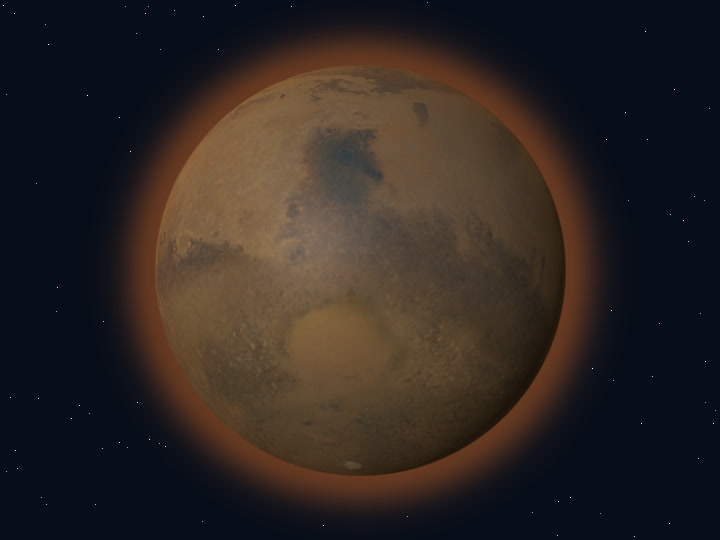
\includegraphics[width=\linewidth,height=4.4cm,keepaspectratio]{imagini/globuri/mars.jpg}\\[2pt]
{\scriptsize\itshape\color{orbitarMuted} Vedere 3D a corpului ceresc (\textbf{Marte})}
&
\centering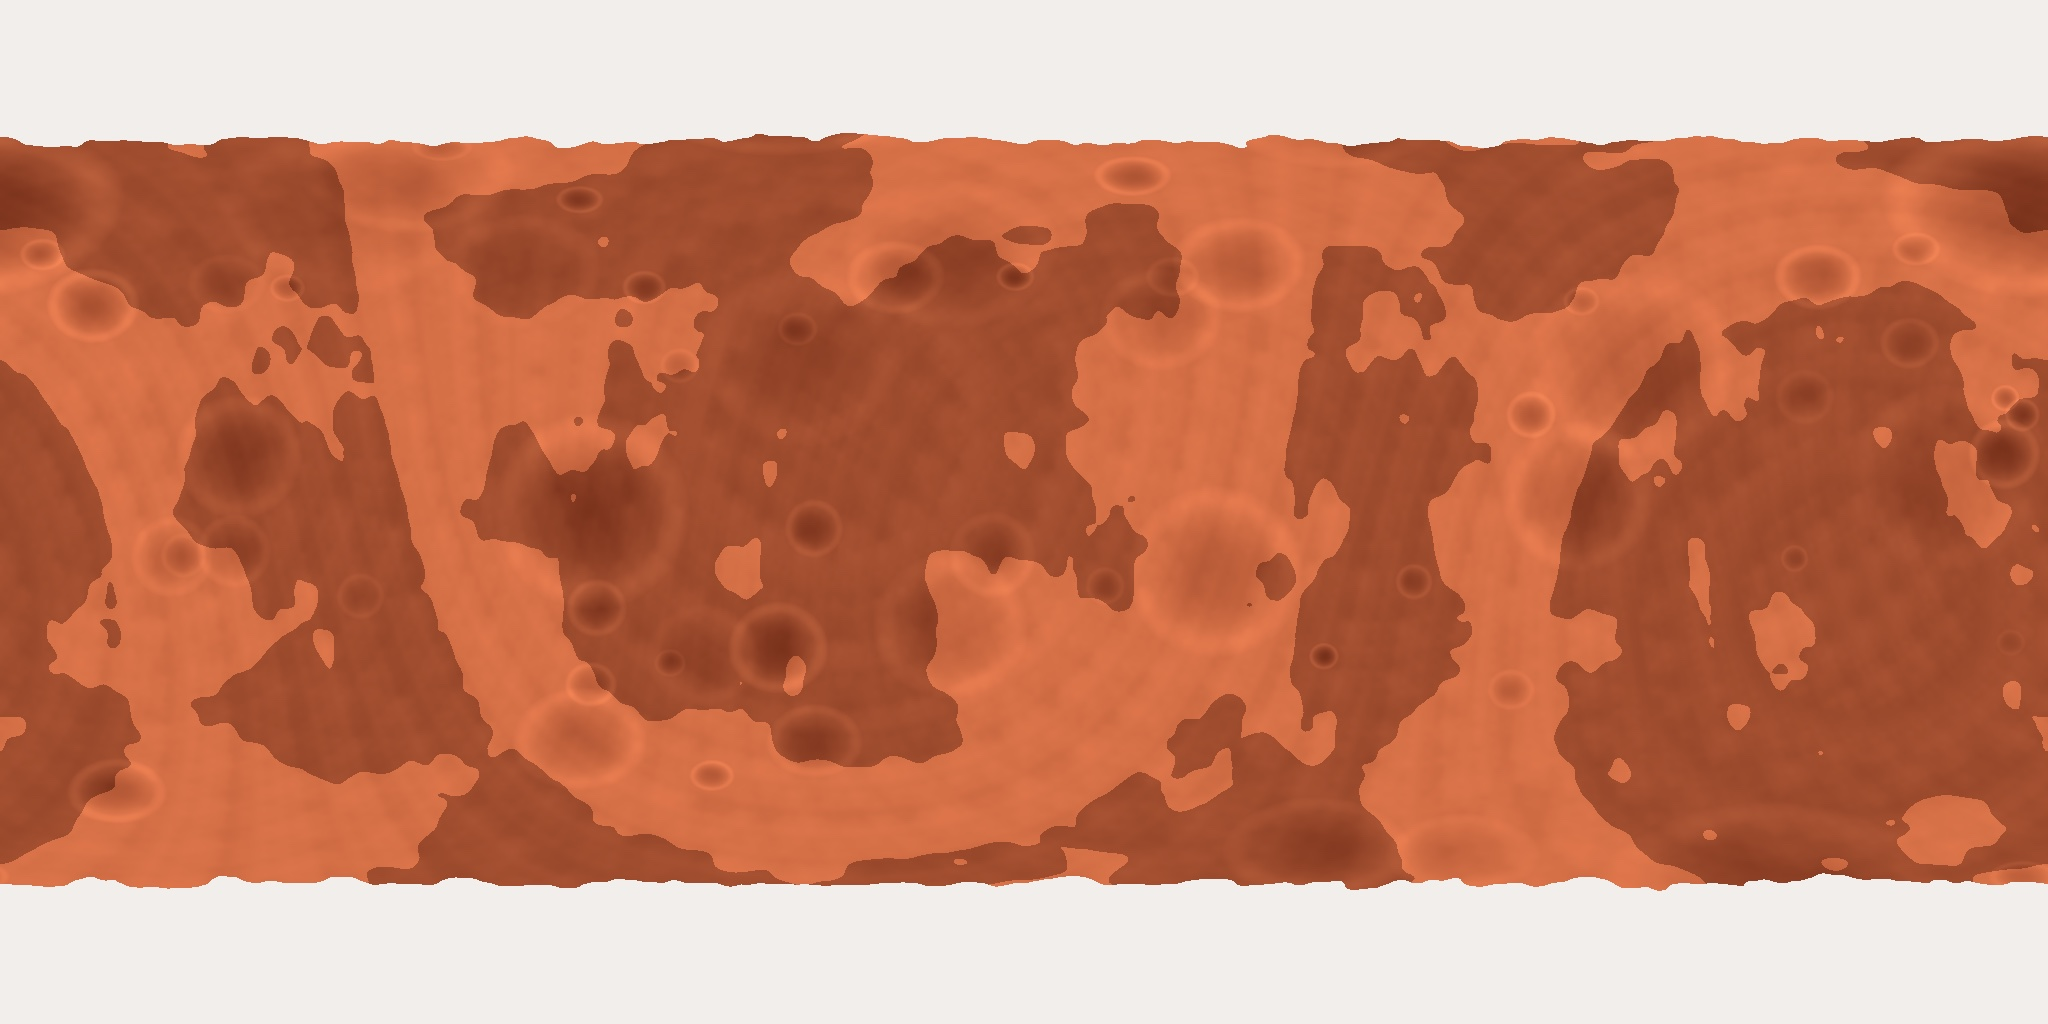
\includegraphics[width=\linewidth,height=4.4cm,keepaspectratio]{../public/textures/hd/mars_viking_albedo.jpg}\\[2pt]
{\scriptsize\itshape\color{orbitarMuted} Planiglob desfășurat: Harta globală a Planetei Roșii Marte (mozaic NASA Viking / MOLA), evidențiind Valles Marineris și regiunea vulcanică Tharsis.}
\end{tabular}
\end{center}


\begin{tcolorbox}[orbitardata, title={\textbf{Repere esențiale: Marte}}]
\small
\begin{itemize}[leftmargin=1.4em, itemsep=2pt, topsep=2pt]
  \item \textbf{Clasificare și orbită:} Planetă Telurică (Stâncoasă) \quad$\bullet$\quad \textbf{Distanță:} 1,524 UA ($\approx$ 228 milioane de kilometri)
  \item \textbf{Dimensiuni și masă:} rază medie 3.389,5 de kilometri \quad$\bullet$\quad masă: 0,107 $\times M_\oplus$
  \item \textbf{Gravitație și regim termic:} 0,380 $\times g_\oplus$ (3,73 m/s$^2$) \quad$\bullet$\quad temperatură medie: -63 $^\circ$C (înclinarea axei: 25,19$^\circ$)
  \item \textbf{Ciclu orbital și rotație:} perioadă orbitală (an): 686,98 zile ($\approx$ 1,88 ani pământești) \quad$\bullet$\quad rotație (zi): 24,62 ore (1,03 zile pământești)
  \item \textbf{Durata călătoriei de pe Pământ:} cu viteza luminii ($1c$): \emph{între 3 și 22 de minute}; cu racheta ($50.000$ de kilometri pe oră): \emph{7 luni}; cu avionul ($900$ de kilometri pe oră): \emph{7 ani}; cu mașina ($100$ de kilometri pe oră): \emph{62 de ani (la apropierea minimă)}.
  \item \textbf{Repere de scară și curiozitate:} Marte este cam pe jumătate cât Pământul: dacă Pământul ar fi o portocală, Marte ar fi o caisă roșiatică! Pe Marte se află Olympus Mons, un vulcan stins de trei ori mai înalt decât vârful Everest!
\end{itemize}
\end{tcolorbox}

\subsubsection*{Prezentare generală și profil astrofizic}
A patra planetă de la Soare are o zi solară (numită \guillemotleft{}sol\guillemotright{}) de 24 de ore și 39 de minute, foarte apropiată de cea terestră. Văile râurilor secate și mineralele hidratate demonstrează că Marte a avut oceane de apă lichidă acum peste 3,5 miliarde de ani. Marte este numită Planeta Roșie deoarece solul ei este plin de praf de fier ruginit! Este singura planetă locuită exclusiv de roboți și rovere trimise de oameni. Marte este cam pe jumătate cât Pământul: dacă Pământul ar fi o portocală, Marte ar fi o caisă roșiatică!

\subsubsection*{Alcătuirea fizică și structura internă}
Privind în profunzimea sa, alcătuirea fizică este organizată pe mai multe straturi și regiuni distincte, fiecare având un rol bine definit în evoluția și dinamica acestui obiect cosmic. În primul rând se remarcă \textbf{Nucleu metalic}, compus din fier, nichel și sulf (aproximativ 1.830 de kilometri rază), măsurat cu precizie de sonda InSight. În strânsă legătură cu această componentă se află \textbf{Scoarță bazaltică bogată în oxid de fier}, care găzduiește canionul Valles Marineris (4.000 de kilometri lungime) și calote polare din gheață și CO$_2$ solid. În completarea acestui ansamblu întâlnim \textbf{Atmosferă rarefiată (0,6\% din presiunea terestră)}, alcătuită în proporție de 95\% dioxid de carbon, capabilă totuși să susțină furtuni globale de praf.

\subsubsection*{Observații astronomice și istoricul explorării}
Explorată de sondele Viking, Mars Reconnaissance Orbiter, MAVEN și roverele Sojourner, Spirit, Opportunity, Curiosity și Perseverance. Pe Marte se află Olympus Mons, un vulcan stins de trei ori mai înalt decât vârful Everest!

\vspace{6pt}
\begin{tcolorbox}[orbitarquiz, title={\textbf{Întrebare de verificare \#6: Marte}}]
\textbf{Cum se numește cel mai înalt vulcan de pe Marte și din întregul Sistem Solar?}
\begin{itemize}[leftmargin=2.2em, itemsep=2pt, topsep=4pt]
  \item[$\square$ \textbf{A.}] Mauna Kea
  \item[$\square$ \textbf{B.}] Olympus Mons
  \item[$\square$ \textbf{C.}] Valles Marineris
  \item[$\square$ \textbf{D.}] Maxwell Montes
\end{itemize}
\vspace{2pt}
{\footnotesize\color{orbitarMuted}\textbf{Răspuns corect:} \textbf{B} (Olympus Mons). \emph{Olympus Mons are o altitudine de aproape 22 de kilometri și o bază de aproximativ 600 de kilometri diametru!}}
\end{tcolorbox}
\clearpage


\subsection{Phobos}
\label{sec:body-phobos}
\vspace{-4pt}
{\large\itshape\color{orbitarAccent} Luna interioară în formă de cartof a planetei Marte}\\[4pt]


\begin{center}
\begin{tabular}{@{}m{0.44\textwidth}@{\hspace{0.03\textwidth}}m{0.51\textwidth}@{}}
\centering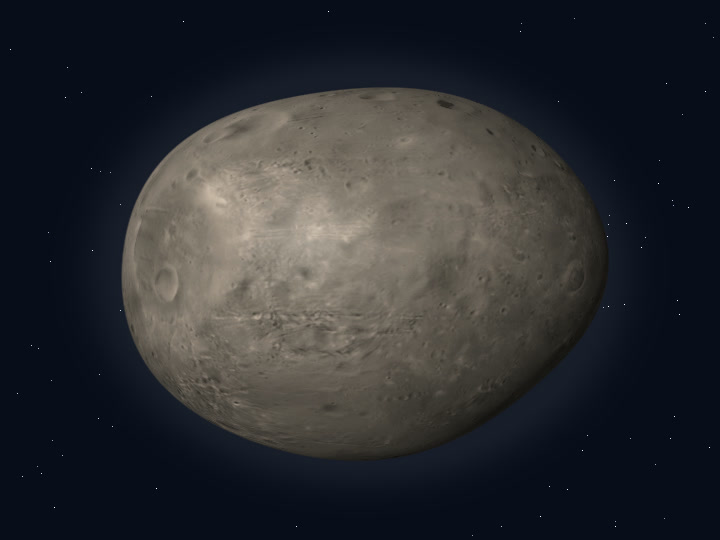
\includegraphics[width=\linewidth,height=4.4cm,keepaspectratio]{imagini/globuri/phobos.jpg}\\[2pt]
{\scriptsize\itshape\color{orbitarMuted} Vedere 3D a corpului ceresc (\textbf{Phobos})}
&
\centering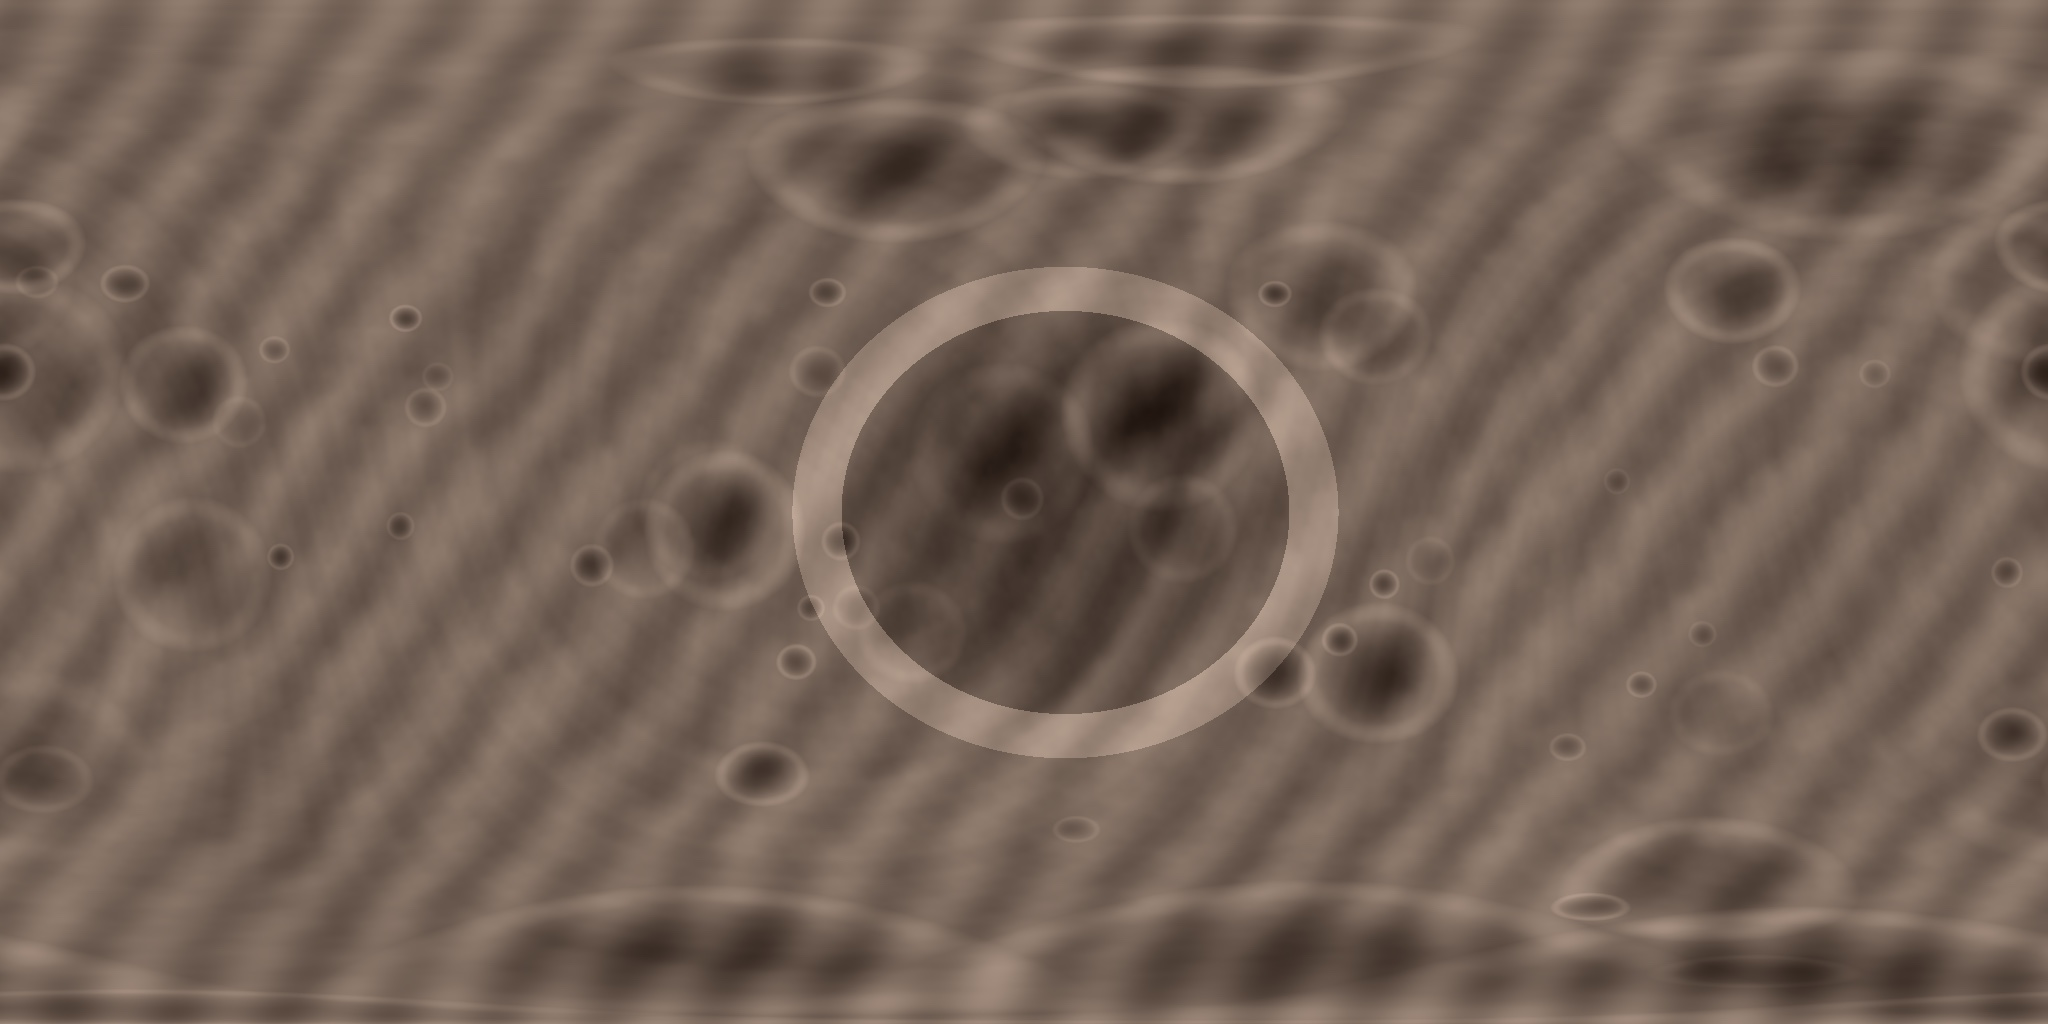
\includegraphics[width=\linewidth,height=4.4cm,keepaspectratio]{../public/textures/hd/phobos_viking.jpg}\\[2pt]
{\scriptsize\itshape\color{orbitarMuted} Planiglob desfășurat: Harta suprafeței satelitul marțian Phobos și a marelui crater Stickney (date NASA Viking).}
\end{tabular}
\end{center}


\begin{tcolorbox}[orbitardata, title={\textbf{Repere esențiale: Phobos}}]
\small
\begin{itemize}[leftmargin=1.4em, itemsep=2pt, topsep=2pt]
  \item \textbf{Clasificare și orbită:} Satelit Natural (Lună) (orbitează în jurul: \textbf{Marte}) \quad$\bullet$\quad \textbf{Distanță:} 1,524 UA ($\approx$ 228 milioane de kilometri)
  \item \textbf{Dimensiuni și masă:} rază medie 11,27 kilometri \quad$\bullet$\quad masă: 1,80e-9 $\times M_\oplus$
  \item \textbf{Gravitație și regim termic:} 0,001 $\times g_\oplus$ (0,01 m/s$^2$) \quad$\bullet$\quad temperatură medie: -40 $^\circ$C (înclinarea axei: Nespecificată)
  \item \textbf{Ciclu orbital și rotație:} perioadă orbitală (an): 0,319 zile pământești \quad$\bullet$\quad rotație (zi): 7,65 ore (0,32 zile pământești)
  \item \textbf{Durata călătoriei de pe Pământ:} cu viteza luminii ($1c$): \emph{între 3 și 22 de minute}; cu racheta ($50.000$ de kilometri pe oră): \emph{7 luni}; cu avionul ($900$ de kilometri pe oră): \emph{7 ani}; cu mașina ($100$ de kilometri pe oră): \emph{62 de ani}.
  \item \textbf{Repere de scară și curiozitate:} Phobos zboară atât de aproape și de repede deasupra lui Marte încât răsare și apune de două ori într-o singură zi marțiană! Pe Phobos se află Craterul Stickney, o urmă de impact atât de uriașă încât aproape a spart mica lună în bucăți!
\end{itemize}
\end{tcolorbox}

\subsubsection*{Prezentare generală și profil astrofizic}
Descoperită în 1877 de astronomul Asaph Hall, Phobos orbitează la numai 6.000 de kilometri deasupra suprafeței marțiene, fiind mai aproape de planeta sa decât orice alt satelit natural din Sistemul Solar. Perioada sa orbitală de 7 ore și 39 de minute este de trei ori mai scurtă decât rotația lui Marte. Phobos este cea mai mare dintre cele două luni ale lui Marte! Nu este rotundă ca Luna noastră, ci are forma unui cartof stâncos plin de cratere și șanțuri. Phobos zboară atât de aproape și de repede deasupra lui Marte încât răsare și apune de două ori într-o singură zi marțiană!

\subsubsection*{Alcătuirea fizică și structura internă}
Privind în profunzimea sa, alcătuirea fizică este organizată pe mai multe straturi și regiuni distincte, fiecare având un rol bine definit în evoluția și dinamica acestui obiect cosmic. În primul rând se remarcă \textbf{Interior poros tip \guillemotleft{}rubble-pile\guillemotright{}}, compus din blocuri de rocă condritică și goluri interne (30\% porozitate), probabil un asteroid capturat. În strânsă legătură cu această componentă se află \textbf{Craterul gigant Stickney (9 kilometri diametru)}, care ocupă aproape jumătate din fața vizibilă a satelitului și este înconjurat de șanțuri paralele de stres. În completarea acestui ansamblu întâlnim \textbf{Strat gros de regolit}, praf fin de până la 100 de metri adâncime, creat de miliarde de ani de bombardament meteoritic.

\subsubsection*{Observații astronomice și istoricul explorării}
Fotografiată de aproape de sondele Mariner 9, Viking 1, Mars Global Surveyor, Mars Express și Mars Reconnaissance Orbiter; ținta viitoarei misiuni japoneze MMX (Martian Moons eXploration). Pe Phobos se află Craterul Stickney, o urmă de impact atât de uriașă încât aproape a spart mica lună în bucăți!

\vspace{6pt}
\begin{tcolorbox}[orbitarquiz, title={\textbf{Întrebare de verificare \#7: Phobos}}]
\textbf{De ce răsare Phobos din vest și apune în est pe cerul planetei Marte?}
\begin{itemize}[leftmargin=2.2em, itemsep=2pt, topsep=4pt]
  \item[$\square$ \textbf{A.}] Pentru că se rotește în jurul lui Marte în 7 ore și 39 de minute, mai repede decât se învârte Marte în jurul axei sale
  \item[$\square$ \textbf{B.}] Pentru că Marte stă pe loc
  \item[$\square$ \textbf{C.}] Din cauza furtunilor de nisip
  \item[$\square$ \textbf{D.}] Pentru că orbitează direct Soarele
\end{itemize}
\vspace{2pt}
{\footnotesize\color{orbitarMuted}\textbf{Răspuns corect:} \textbf{A} (Pentru că se rotește în jurul lui Marte în 7 ore și 39 de minute, mai repede decât se învârte Marte în jurul axei sale). \emph{Phobos înconjoară Marte în doar 7,65 ore, în timp ce o zi pe Marte durează 24,6 ore, deci satelitul depășește rotația planetei.}}
\end{tcolorbox}
\clearpage


\subsection{Deimos}
\label{sec:body-deimos}
\vspace{-4pt}
{\large\itshape\color{orbitarAccent} Luna exterioară, mică și netedă, a planetei Marte}\\[4pt]


\begin{center}
\begin{tabular}{@{}m{0.44\textwidth}@{\hspace{0.03\textwidth}}m{0.51\textwidth}@{}}
\centering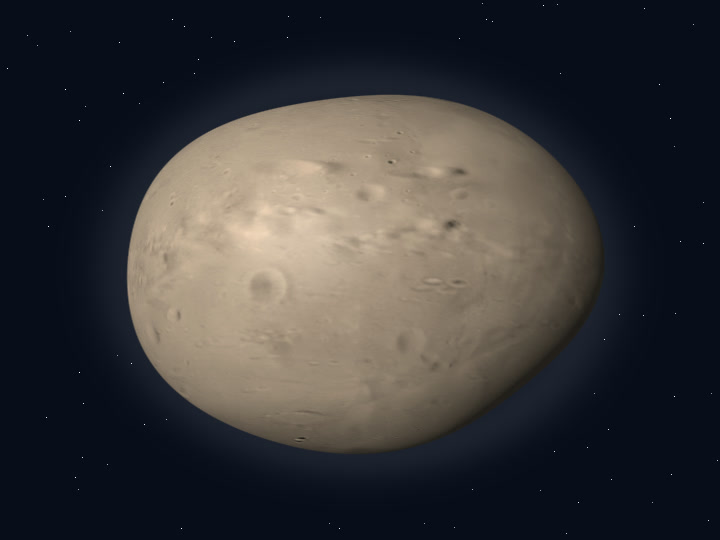
\includegraphics[width=\linewidth,height=4.4cm,keepaspectratio]{imagini/globuri/deimos.jpg}\\[2pt]
{\scriptsize\itshape\color{orbitarMuted} Vedere 3D a corpului ceresc (\textbf{Deimos})}
&
\centering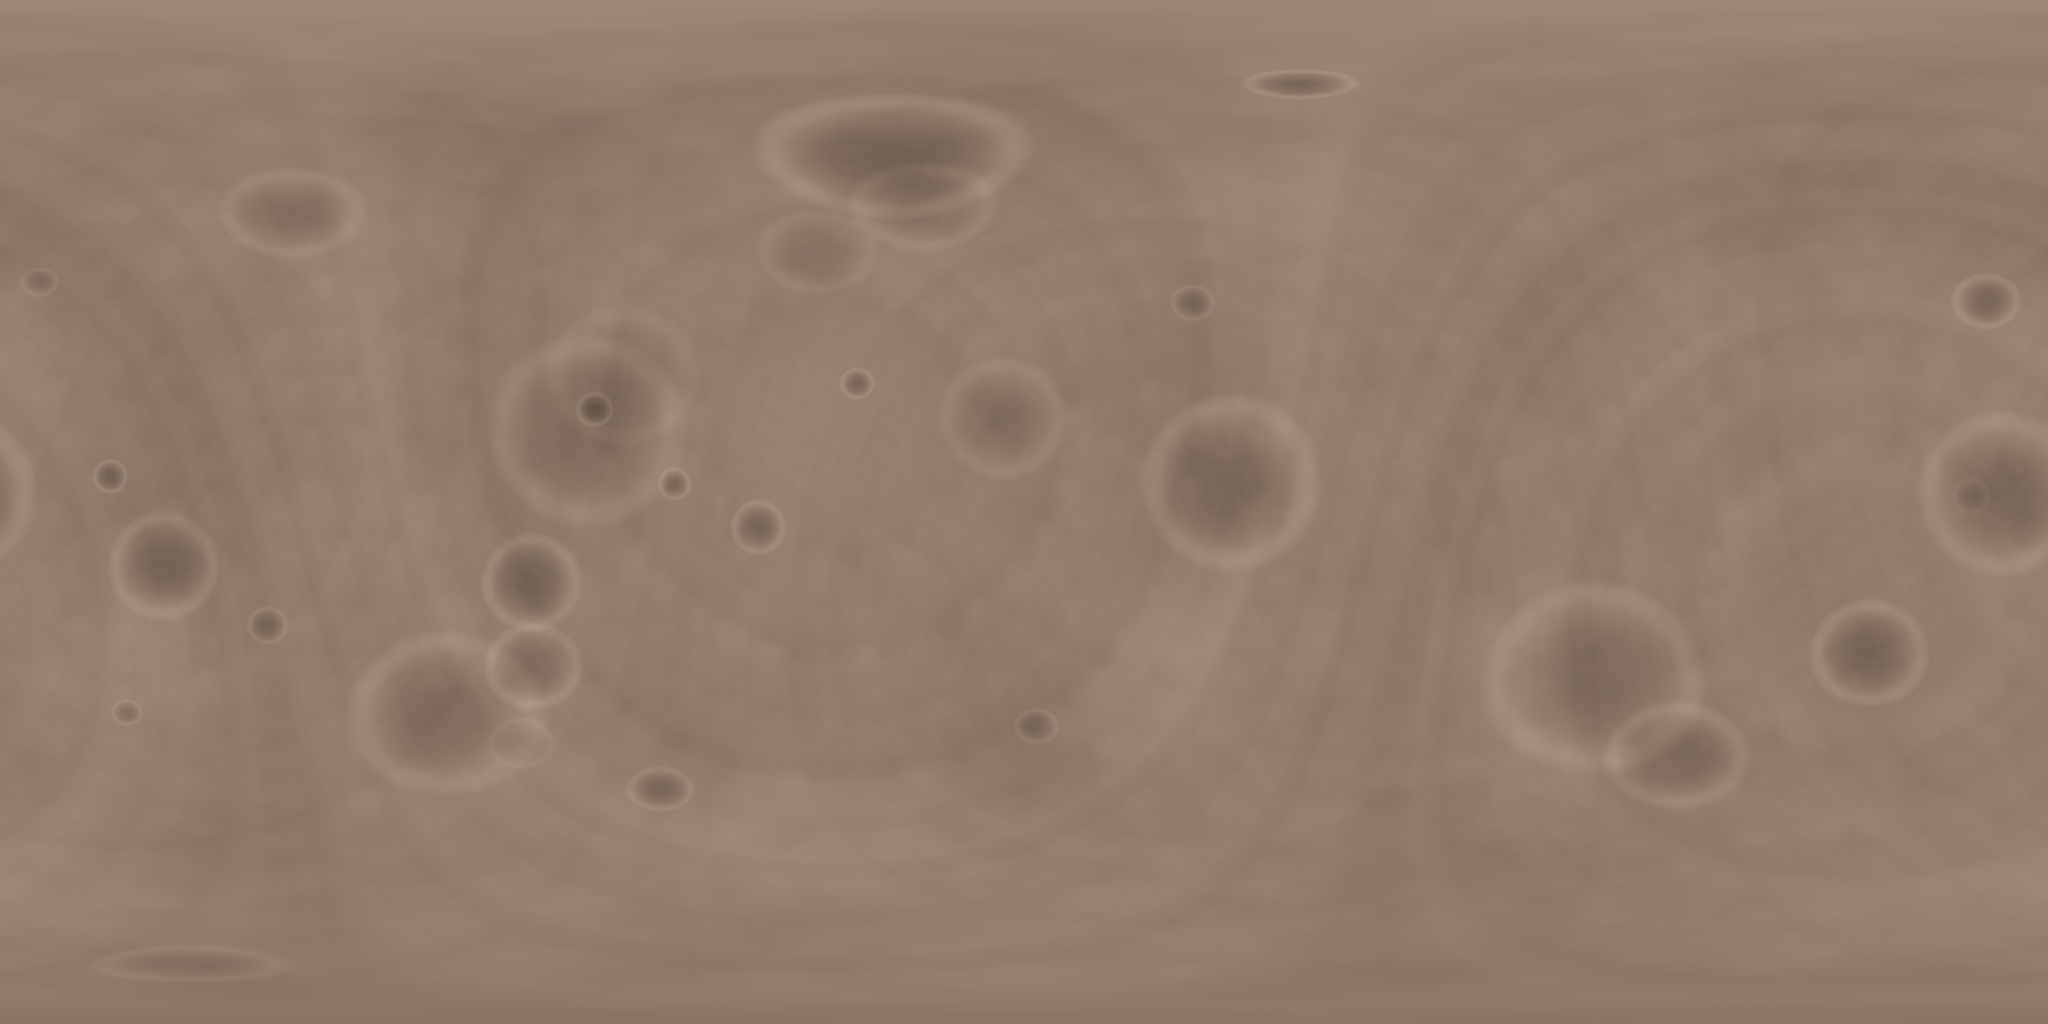
\includegraphics[width=\linewidth,height=4.4cm,keepaspectratio]{../public/textures/hd/deimos_viking.jpg}\\[2pt]
{\scriptsize\itshape\color{orbitarMuted} Planiglob desfășurat: Harta suprafeței netede și prăfuite a lui Deimos, satelitul exterior al lui Marte (date NASA Viking).}
\end{tabular}
\end{center}


\begin{tcolorbox}[orbitardata, title={\textbf{Repere esențiale: Deimos}}]
\small
\begin{itemize}[leftmargin=1.4em, itemsep=2pt, topsep=2pt]
  \item \textbf{Clasificare și orbită:} Satelit Natural (Lună) (orbitează în jurul: \textbf{Marte}) \quad$\bullet$\quad \textbf{Distanță:} 1,524 UA ($\approx$ 228 milioane de kilometri)
  \item \textbf{Dimensiuni și masă:} rază medie 6,2 kilometri \quad$\bullet$\quad masă: 2,50e-10 $\times M_\oplus$
  \item \textbf{Gravitație și regim termic:} Microgravitație / Imponderabilitate ($\approx 0\,g$) \quad$\bullet$\quad temperatură medie: -40 $^\circ$C (înclinarea axei: Nespecificată)
  \item \textbf{Ciclu orbital și rotație:} perioadă orbitală (an): 1,263 zile pământești \quad$\bullet$\quad rotație (zi): 30,31 ore (1,26 zile pământești)
  \item \textbf{Durata călătoriei de pe Pământ:} cu viteza luminii ($1c$): \emph{între 3 și 22 de minute}; cu racheta ($50.000$ de kilometri pe oră): \emph{7 luni}; cu avionul ($900$ de kilometri pe oră): \emph{7 ani}; cu mașina ($100$ de kilometri pe oră): \emph{62 de ani}.
  \item \textbf{Repere de scară și curiozitate:} Gravitația pe Deimos este atât de mică încât, dacă ai alerga repede și ai sări, te-ai desprinde de sol și ai pluti direct în spațiu! Văzut de pe suprafața lui Marte, Deimos pare doar o stea foarte strălucitoare, puțin mai mare decât planeta Venus!
\end{itemize}
\end{tcolorbox}

\subsubsection*{Prezentare generală și profil astrofizic}
Descoperită tot de Asaph Hall în august 1877, Deimos orbitează la 23.460 de kilometri de centrul lui Marte în 30,3 ore. Cu o rază medie de doar 6,2 kilometri, este unul dintre cei mai mici sateliți cunoscuți din Sistemul Solar. Deimos este fratele mai mic al lui Phobos și a doua lună a lui Marte! Este o stâncă mică, acoperită cu o pătură groasă de praf fin care îi netezește craterele. Gravitația pe Deimos este atât de mică încât, dacă ai alerga repede și ai sări, te-ai desprinde de sol și ai pluti direct în spațiu!

\subsubsection*{Alcătuirea fizică și structura internă}
Privind în profunzimea sa, alcătuirea fizică este organizată pe mai multe straturi și regiuni distincte, fiecare având un rol bine definit în evoluția și dinamica acestui obiect cosmic. În primul rând se remarcă \textbf{Corp condritic bogat în carbon}, densitate scăzută de 1,47 g/cm$^3$, similară asteroizilor de tip C și D din centura exterioară. În strânsă legătură cu această componentă se află \textbf{Craterele Swift și Voltaire}, cele două cratere principale (de aproximativ 1--3 kilometri lărgime), numite după scriitorii care au imaginat două luni marțiene înainte de descoperirea lor. În completarea acestui ansamblu întâlnim \textbf{Manta netedă de regolit}, unde craterele sunt parțial umplute cu praf marțian-asteroidal, oferind un relief mult mai blând decât cel de pe Phobos.

\subsubsection*{Observații astronomice și istoricul explorării}
Fotografiată în detaliu de sonda Viking 2 în 1977 (de la numai 30 de kilometri distanță), de Mars Reconnaissance Orbiter și în 2023 de sonda Emiratelor Arabe Unite \guillemotleft{}Hope\guillemotright{} (Al-Amal). Văzut de pe suprafața lui Marte, Deimos pare doar o stea foarte strălucitoare, puțin mai mare decât planeta Venus!

\vspace{6pt}
\begin{tcolorbox}[orbitarquiz, title={\textbf{Întrebare de verificare \#8: Deimos}}]
\textbf{Cum arată suprafața satelitului Deimos în comparație cu cea a lui Phobos?}
\begin{itemize}[leftmargin=2.2em, itemsep=2pt, topsep=4pt]
  \item[$\square$ \textbf{A.}] Este acoperită cu gheață albastră
  \item[$\square$ \textbf{B.}] Este mult mai netedă, deoarece craterele sunt umplute cu un strat gros de praf (regolit)
  \item[$\square$ \textbf{C.}] Are vulcani activi
  \item[$\square$ \textbf{D.}] Este perfect rotundă ca o bilă de oțel
\end{itemize}
\vspace{2pt}
{\footnotesize\color{orbitarMuted}\textbf{Răspuns corect:} \textbf{B} (Este mult mai netedă, deoarece craterele sunt umplute cu un strat gros de praf (regolit)). \emph{Deimos este acoperit cu un strat gros de regolit pulverulent care a umplut craterele vechi, dându-i un aspect catifelat.}}
\end{tcolorbox}
\clearpage


\section{Jupiter}
\label{sec:body-jupiter}
\vspace{-4pt}
{\large\itshape\color{orbitarAccent} Cel mai masiv gigant gazos din Sistemul Solar}\\[4pt]


\begin{center}
\begin{tabular}{@{}m{0.44\textwidth}@{\hspace{0.03\textwidth}}m{0.51\textwidth}@{}}
\centering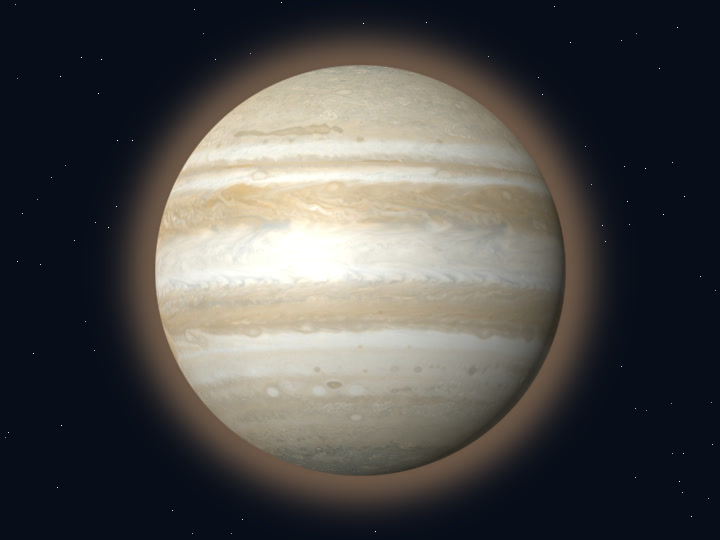
\includegraphics[width=\linewidth,height=4.4cm,keepaspectratio]{imagini/globuri/jupiter.jpg}\\[2pt]
{\scriptsize\itshape\color{orbitarMuted} Vedere 3D a corpului ceresc (\textbf{Jupiter})}
&
\centering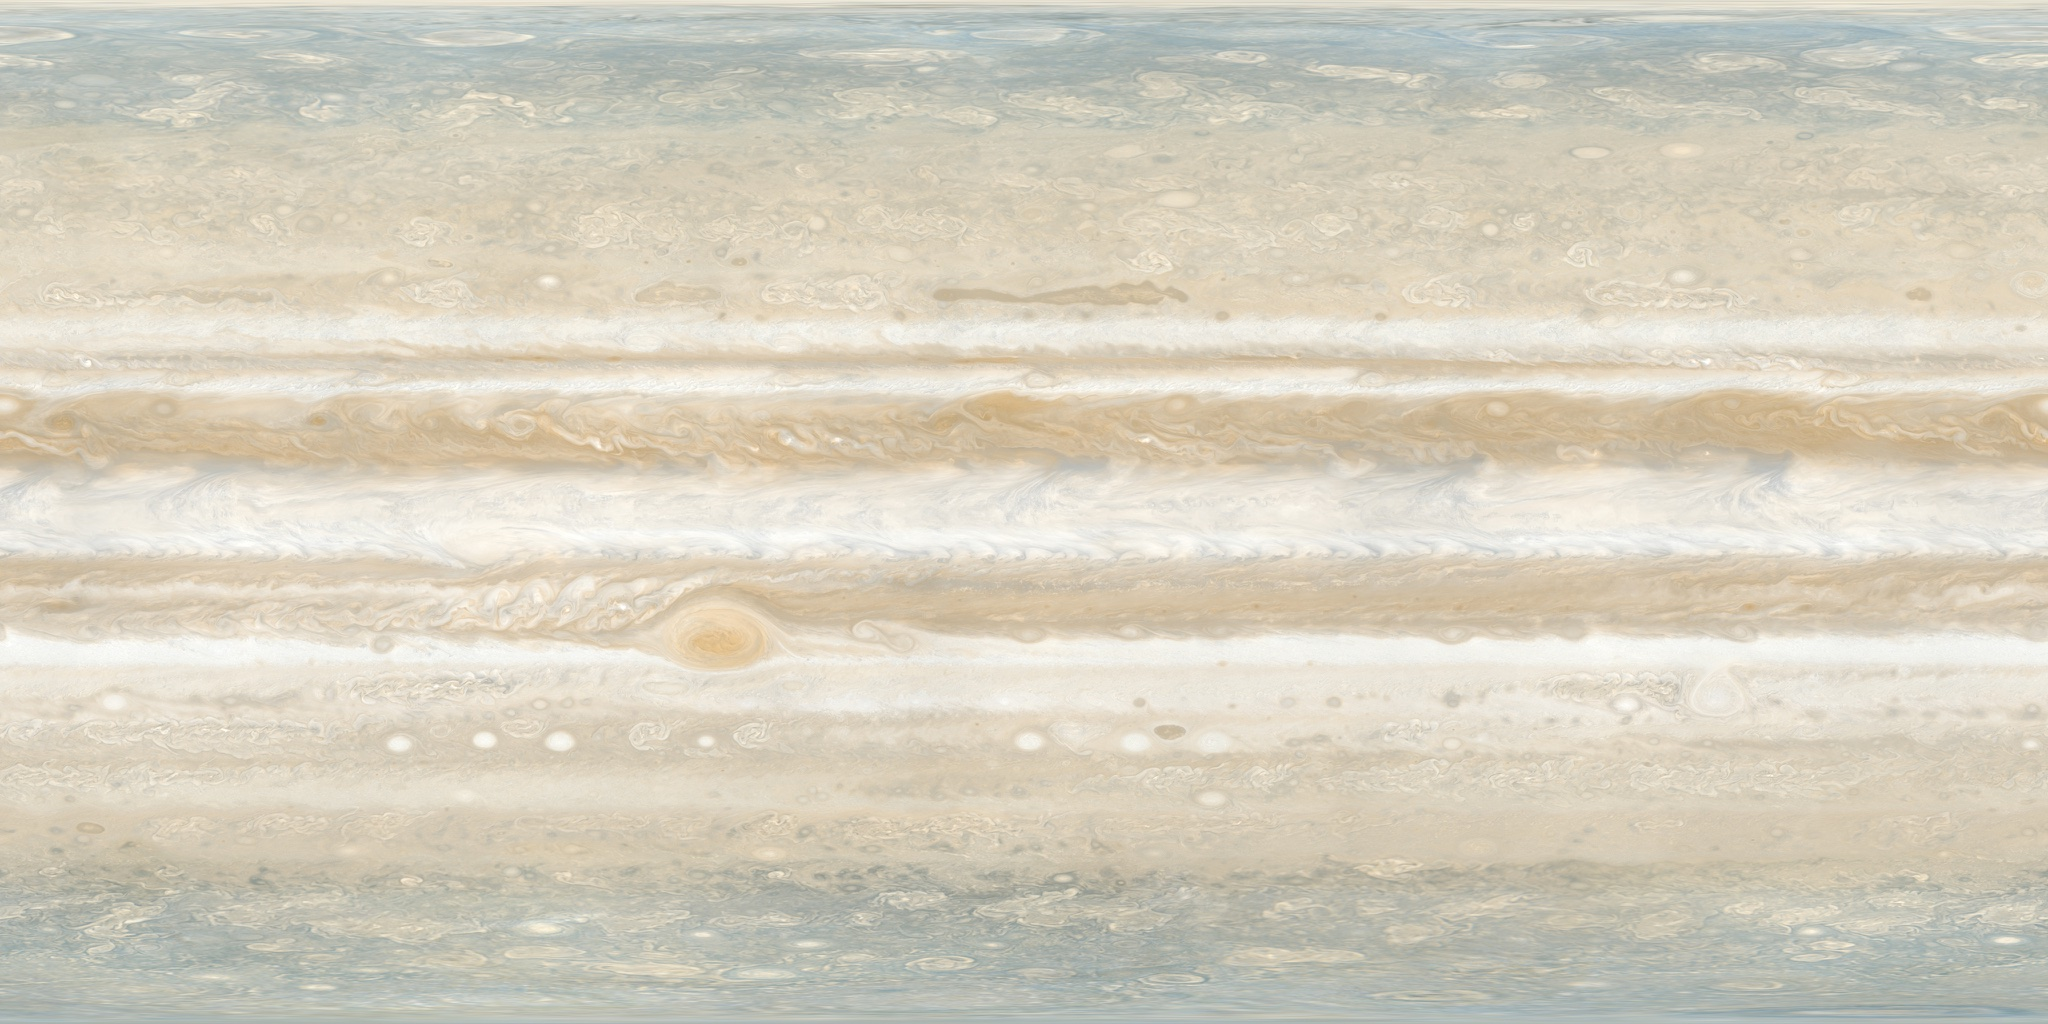
\includegraphics[width=\linewidth,height=4.4cm,keepaspectratio]{../public/textures/hd/jupiter_cassini_albedo.jpg}\\[2pt]
{\scriptsize\itshape\color{orbitarMuted} Planiglob desfășurat: Harta globală a benzilor de nori și a Marii Pete Roșii de pe Jupiter, fotografiată de sonda NASA/ESA Cassini.}
\end{tabular}
\end{center}


\begin{tcolorbox}[orbitardata, title={\textbf{Repere esențiale: Jupiter}}]
\small
\begin{itemize}[leftmargin=1.4em, itemsep=2pt, topsep=2pt]
  \item \textbf{Clasificare și orbită:} Gigant Gazos \quad$\bullet$\quad \textbf{Distanță:} 5,204 UA ($\approx$ 779 milioane de kilometri)
  \item \textbf{Dimensiuni și masă:} rază medie 69.911 kilometri \quad$\bullet$\quad masă: 317,800 $\times M_\oplus$
  \item \textbf{Gravitație și regim termic:} 2,530 $\times g_\oplus$ (24,82 m/s$^2$) \quad$\bullet$\quad temperatură medie: -110 $^\circ$C (înclinarea axei: 3,13$^\circ$)
  \item \textbf{Ciclu orbital și rotație:} perioadă orbitală (an): 4.332,59 zile ($\approx$ 11,86 ani pământești) \quad$\bullet$\quad rotație (zi): 9,93 ore (0,41 zile pământești)
  \item \textbf{Durata călătoriei de pe Pământ:} cu viteza luminii ($1c$): \emph{35 de minute}; cu racheta ($50.000$ de kilometri pe oră): \emph{2 până la 5 ani}; cu avionul ($900$ de kilometri pe oră): \emph{80 de ani}; cu mașina ($100$ de kilometri pe oră): \emph{717 ani}.
  \item \textbf{Repere de scară și curiozitate:} Dacă Pământul ar fi un bob de strugure, Jupiter ar fi cât un pepene verde imens! Marea Pată Roșie de pe Jupiter este o furtună gigantică ce suflă de sute de ani și e mai mare decât tot Pământul!
\end{itemize}
\end{tcolorbox}

\subsubsection*{Prezentare generală și profil astrofizic}
Jupiter are o masă de 2,5 ori mai mare decât a tuturor celorlalte planete la un loc. Se rotește în jurul axei sale în mai puțin de 10 ore, ceea ce creează benzi atmosferice spectaculoase (zone și centuri) și cel mai puternic câmp magnetic planetar. Jupiter este uriașul protector al Sistemului Solar! Nu are un sol tare pe care să poți păși, fiind alcătuit aproape în întregime din nori și gaze. Dacă Pământul ar fi un bob de strugure, Jupiter ar fi cât un pepene verde imens!

\subsubsection*{Alcătuirea fizică și structura internă}
Privind în profunzimea sa, alcătuirea fizică este organizată pe mai multe straturi și regiuni distincte, fiecare având un rol bine definit în evoluția și dinamica acestui obiect cosmic. În primul rând se remarcă \textbf{Nucleu difuz stâncos și de gheață}, un nucleu central de mare presiune amestecat cu hidrogen metalic. În strânsă legătură cu această componentă se află \textbf{Ocean de hidrogen metalic lichid}, unde la presiuni de milioane de atmosfere, hidrogenul devine conductor electric și generează magnetosfera uriașă. În completarea acestui ansamblu întâlnim \textbf{Atmosferă de hidrogen (90\%) și heliu (10\%)}, nori de amoniac și hidrosulfură de amoniu organizați în jeturi zonale și anticicloane.

\subsubsection*{Observații astronomice și istoricul explorării}
Survolată de Pioneer 10/11, Voyager 1/2, Ulysses, Cassini și New Horizons; studiată pe orbită de sondele Galileo (1995--2003) și Juno (din 2016). Marea Pată Roșie de pe Jupiter este o furtună gigantică ce suflă de sute de ani și e mai mare decât tot Pământul!

\vspace{6pt}
\begin{tcolorbox}[orbitarquiz, title={\textbf{Întrebare de verificare \#9: Jupiter}}]
\textbf{Ce este celebra \guillemotleft{}Mare Pată Roșie\guillemotright{} de pe Jupiter?}
\begin{itemize}[leftmargin=2.2em, itemsep=2pt, topsep=4pt]
  \item[$\square$ \textbf{A.}] Un vulcan uriaș de lavă
  \item[$\square$ \textbf{B.}] Un ocean de fier lichid
  \item[$\square$ \textbf{C.}] O furtună anticiclonică mai mare decât Pământul
  \item[$\square$ \textbf{D.}] Un crater de impact
\end{itemize}
\vspace{2pt}
{\footnotesize\color{orbitarMuted}\textbf{Răspuns corect:} \textbf{C} (O furtună anticiclonică mai mare decât Pământul). \emph{Marea Pată Roșie este un anticiclon gigantic cu vânturi de peste 430 kilometri pe oră, observat de mai bine de 300 de ani.}}
\end{tcolorbox}
\clearpage


\subsection{Io}
\label{sec:body-io}
\vspace{-4pt}
{\large\itshape\color{orbitarAccent} Luna vulcanică a lui Jupiter}\\[4pt]


\begin{center}
\begin{tabular}{@{}m{0.44\textwidth}@{\hspace{0.03\textwidth}}m{0.51\textwidth}@{}}
\centering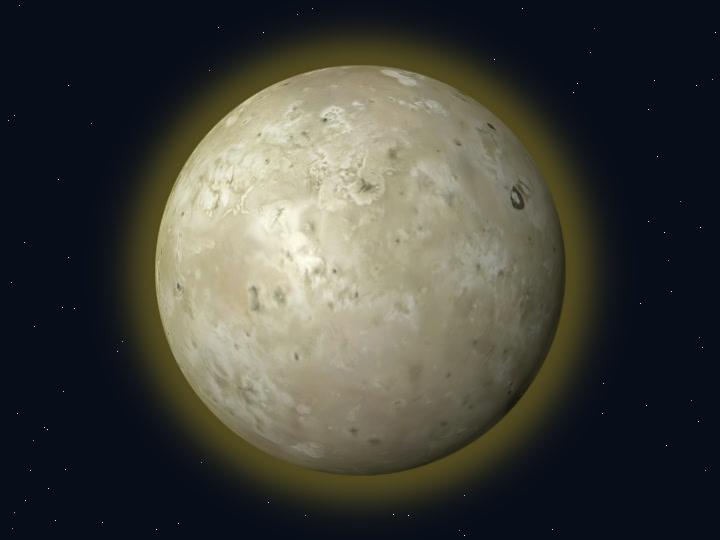
\includegraphics[width=\linewidth,height=4.4cm,keepaspectratio]{imagini/globuri/io.jpg}\\[2pt]
{\scriptsize\itshape\color{orbitarMuted} Vedere 3D a corpului ceresc (\textbf{Io})}
&
\centering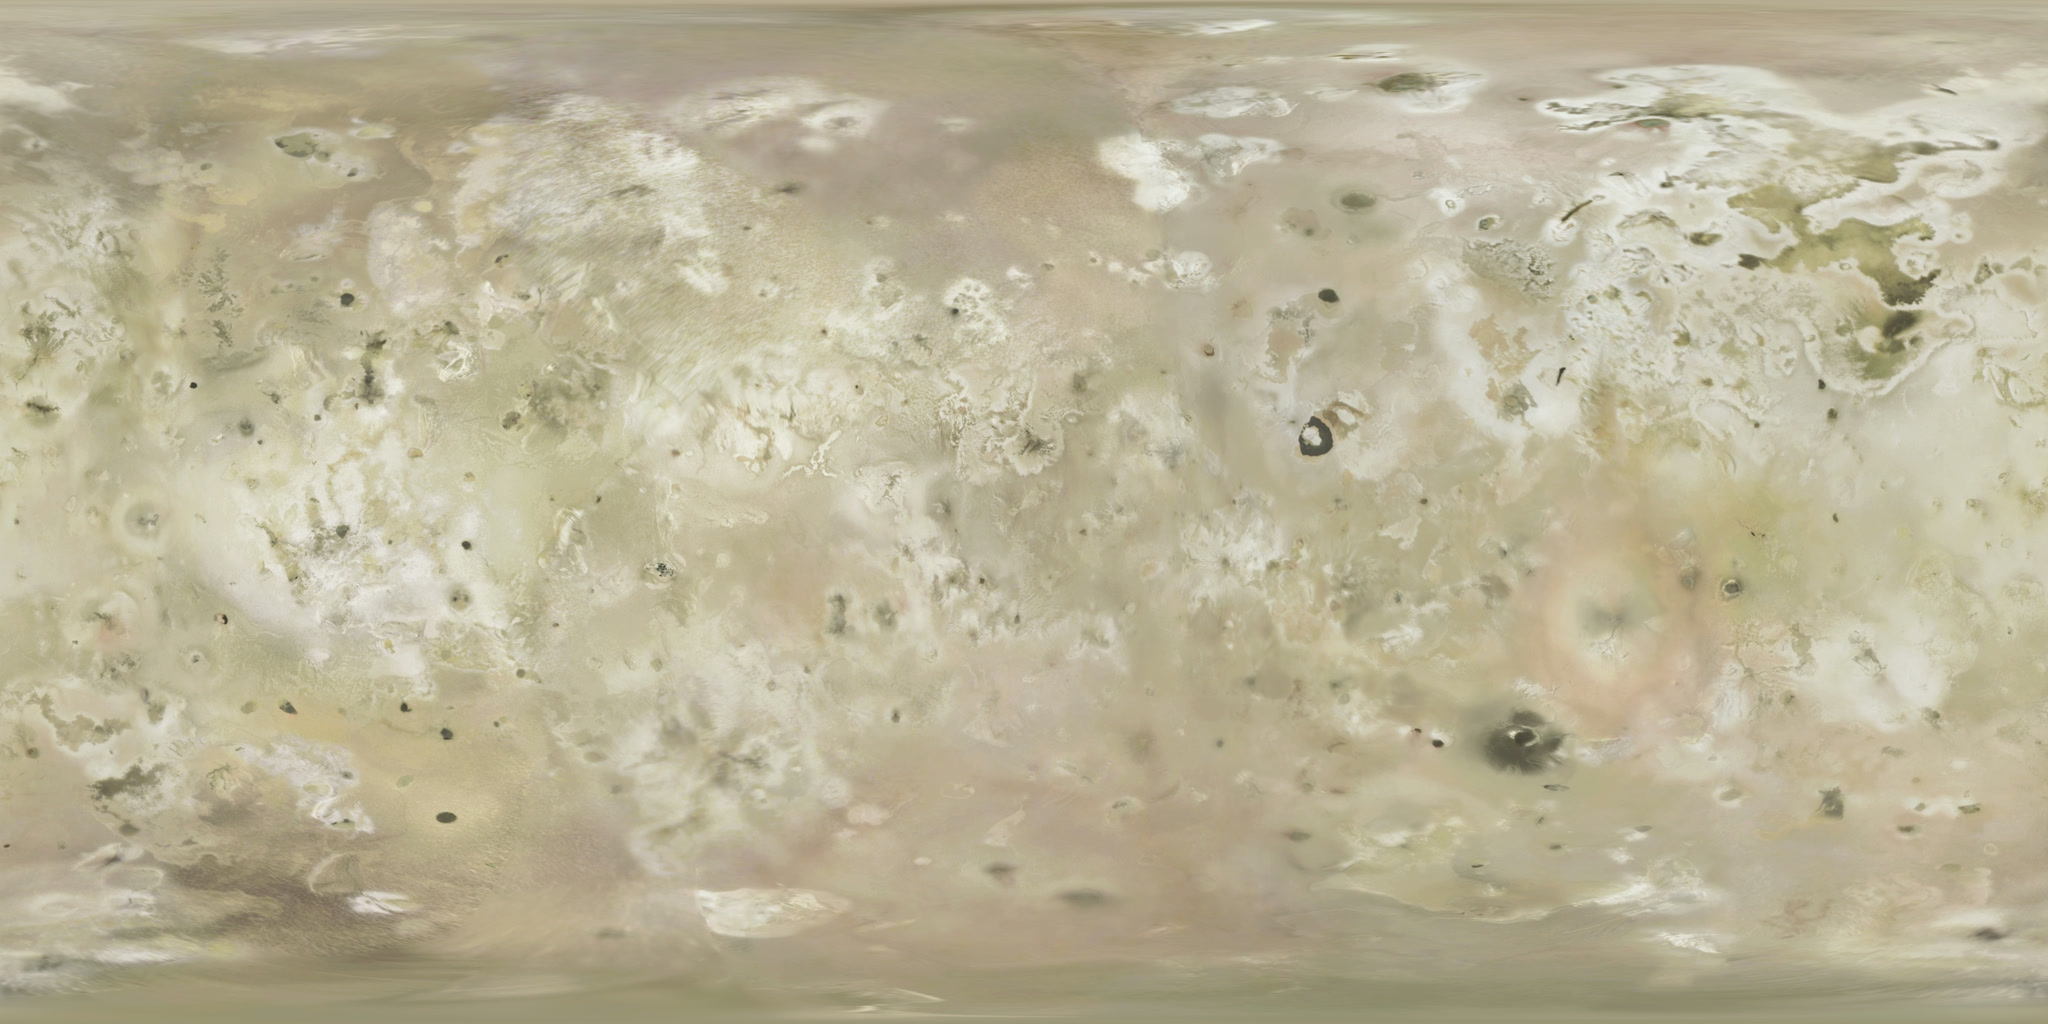
\includegraphics[width=\linewidth,height=4.4cm,keepaspectratio]{../public/textures/hd/io_galileo.jpg}\\[2pt]
{\scriptsize\itshape\color{orbitarMuted} Planiglob desfășurat: Harta vulcanică globală a lunii Io, acoperită cu depozite de sulf și caldere active (sonda NASA Galileo).}
\end{tabular}
\end{center}


\begin{tcolorbox}[orbitardata, title={\textbf{Repere esențiale: Io}}]
\small
\begin{itemize}[leftmargin=1.4em, itemsep=2pt, topsep=2pt]
  \item \textbf{Clasificare și orbită:} Satelit Natural (Lună) (orbitează în jurul: \textbf{Jupiter}) \quad$\bullet$\quad \textbf{Distanță:} 5,204 UA ($\approx$ 779 milioane de kilometri)
  \item \textbf{Dimensiuni și masă:} rază medie 1.821,6 de kilometri \quad$\bullet$\quad masă: 0,015 $\times M_\oplus$
  \item \textbf{Gravitație și regim termic:} 0,183 $\times g_\oplus$ (1,80 m/s$^2$) \quad$\bullet$\quad temperatură medie: -143 $^\circ$C (înclinarea axei: Nespecificată)
  \item \textbf{Ciclu orbital și rotație:} perioadă orbitală (an): 1,769 zile pământești \quad$\bullet$\quad rotație (zi): 42,46 ore (1,77 zile pământești)
  \item \textbf{Durata călătoriei de pe Pământ:} cu viteza luminii ($1c$): \emph{35 de minute}; cu racheta ($50.000$ de kilometri pe oră): \emph{2,5 ani}; cu avionul ($900$ de kilometri pe oră): \emph{80 de ani}; cu mașina ($100$ de kilometri pe oră): \emph{717 ani}.
  \item \textbf{Repere de scară și curiozitate:} Cu petele ei galbene, portocalii și roșii, Io arată exact ca o pizza uriașă cu multă brânză! Jupiter și celelalte luni trag atât de tare de Io încât interiorul ei se frământă și se încălzește ca o bucată de plastilină!
\end{itemize}
\end{tcolorbox}

\subsubsection*{Prezentare generală și profil astrofizic}
Cel mai apropiat dintre cei patru sateliți galileeni ai lui Jupiter suferă o încălzire mareică extremă din cauza rezonanței orbitale 4:2:1 cu Europa și Ganymede. Are peste 400 de vulcani activi, iar jeturile sale eruptive se ridică până la 500 de kilometri altitudine. Io este cea mai vulcanică lume din tot Sistemul Solar! Are sute de vulcani activi care aruncă fântâni uriașe de lavă și sulf până în spațiu. Cu petele ei galbene, portocalii și roșii, Io arată exact ca o pizza uriașă cu multă brânză!

\subsubsection*{Alcătuirea fizică și structura internă}
Privind în profunzimea sa, alcătuirea fizică este organizată pe mai multe straturi și regiuni distincte, fiecare având un rol bine definit în evoluția și dinamica acestui obiect cosmic. În primul rând se remarcă \textbf{Nucleu de fier și sulfură de fier}, care reprezintă aproximativ 20\% din masa satelitului. În strânsă legătură cu această componentă se află \textbf{Manta de silicați și ocean de magmă}, un strat global de magmă topită la 50 de kilometri sub scoarță, alimentat de frecarea mareică. În completarea acestui ansamblu întâlnim \textbf{Scoarță bogată în sulf}, câmpii de lavă și caldere vulcanice precum Loki Patera, fără cratere de impact vizibile.

\subsubsection*{Observații astronomice și istoricul explorării}
Descoperită de Galileo Galilei în 1610; vulcanismul ei activ a fost observat pentru prima dată de sonda Voyager 1 în 1979. Jupiter și celelalte luni trag atât de tare de Io încât interiorul ei se frământă și se încălzește ca o bucată de plastilină!

\vspace{6pt}
\begin{tcolorbox}[orbitarquiz, title={\textbf{Întrebare de verificare \#10: Io}}]
\textbf{Ce fenomen provoacă activitatea vulcanică extremă de pe satelitul Io?}
\begin{itemize}[leftmargin=2.2em, itemsep=2pt, topsep=4pt]
  \item[$\square$ \textbf{A.}] Căldura directă de la Soare
  \item[$\square$ \textbf{B.}] Încălzirea mareică produsă de gravitația lui Jupiter și a lunilor vecine
  \item[$\square$ \textbf{C.}] Impactul continuu cu asteroizi
  \item[$\square$ \textbf{D.}] Fuziunea nucleară
\end{itemize}
\vspace{2pt}
{\footnotesize\color{orbitarMuted}\textbf{Răspuns corect:} \textbf{B} (Încălzirea mareică produsă de gravitația lui Jupiter și a lunilor vecine). \emph{Forțele mareice uriașe ale lui Jupiter deformează continuu interiorul lui Io, generând căldură prin frecare internă.}}
\end{tcolorbox}
\clearpage


\subsection{Europa}
\label{sec:body-europa}
\vspace{-4pt}
{\large\itshape\color{orbitarAccent} Luna înghețată a lui Jupiter cu un ocean ascuns}\\[4pt]


\begin{center}
\begin{tabular}{@{}m{0.44\textwidth}@{\hspace{0.03\textwidth}}m{0.51\textwidth}@{}}
\centering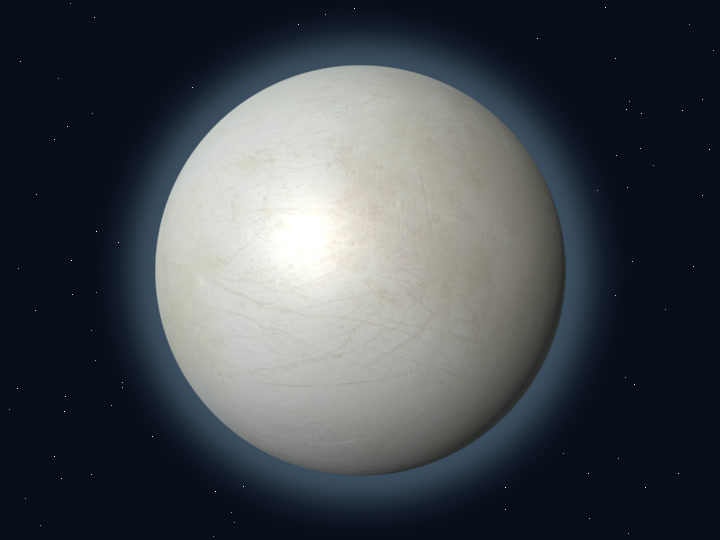
\includegraphics[width=\linewidth,height=4.4cm,keepaspectratio]{imagini/globuri/europa.jpg}\\[2pt]
{\scriptsize\itshape\color{orbitarMuted} Vedere 3D a corpului ceresc (\textbf{Europa})}
&
\centering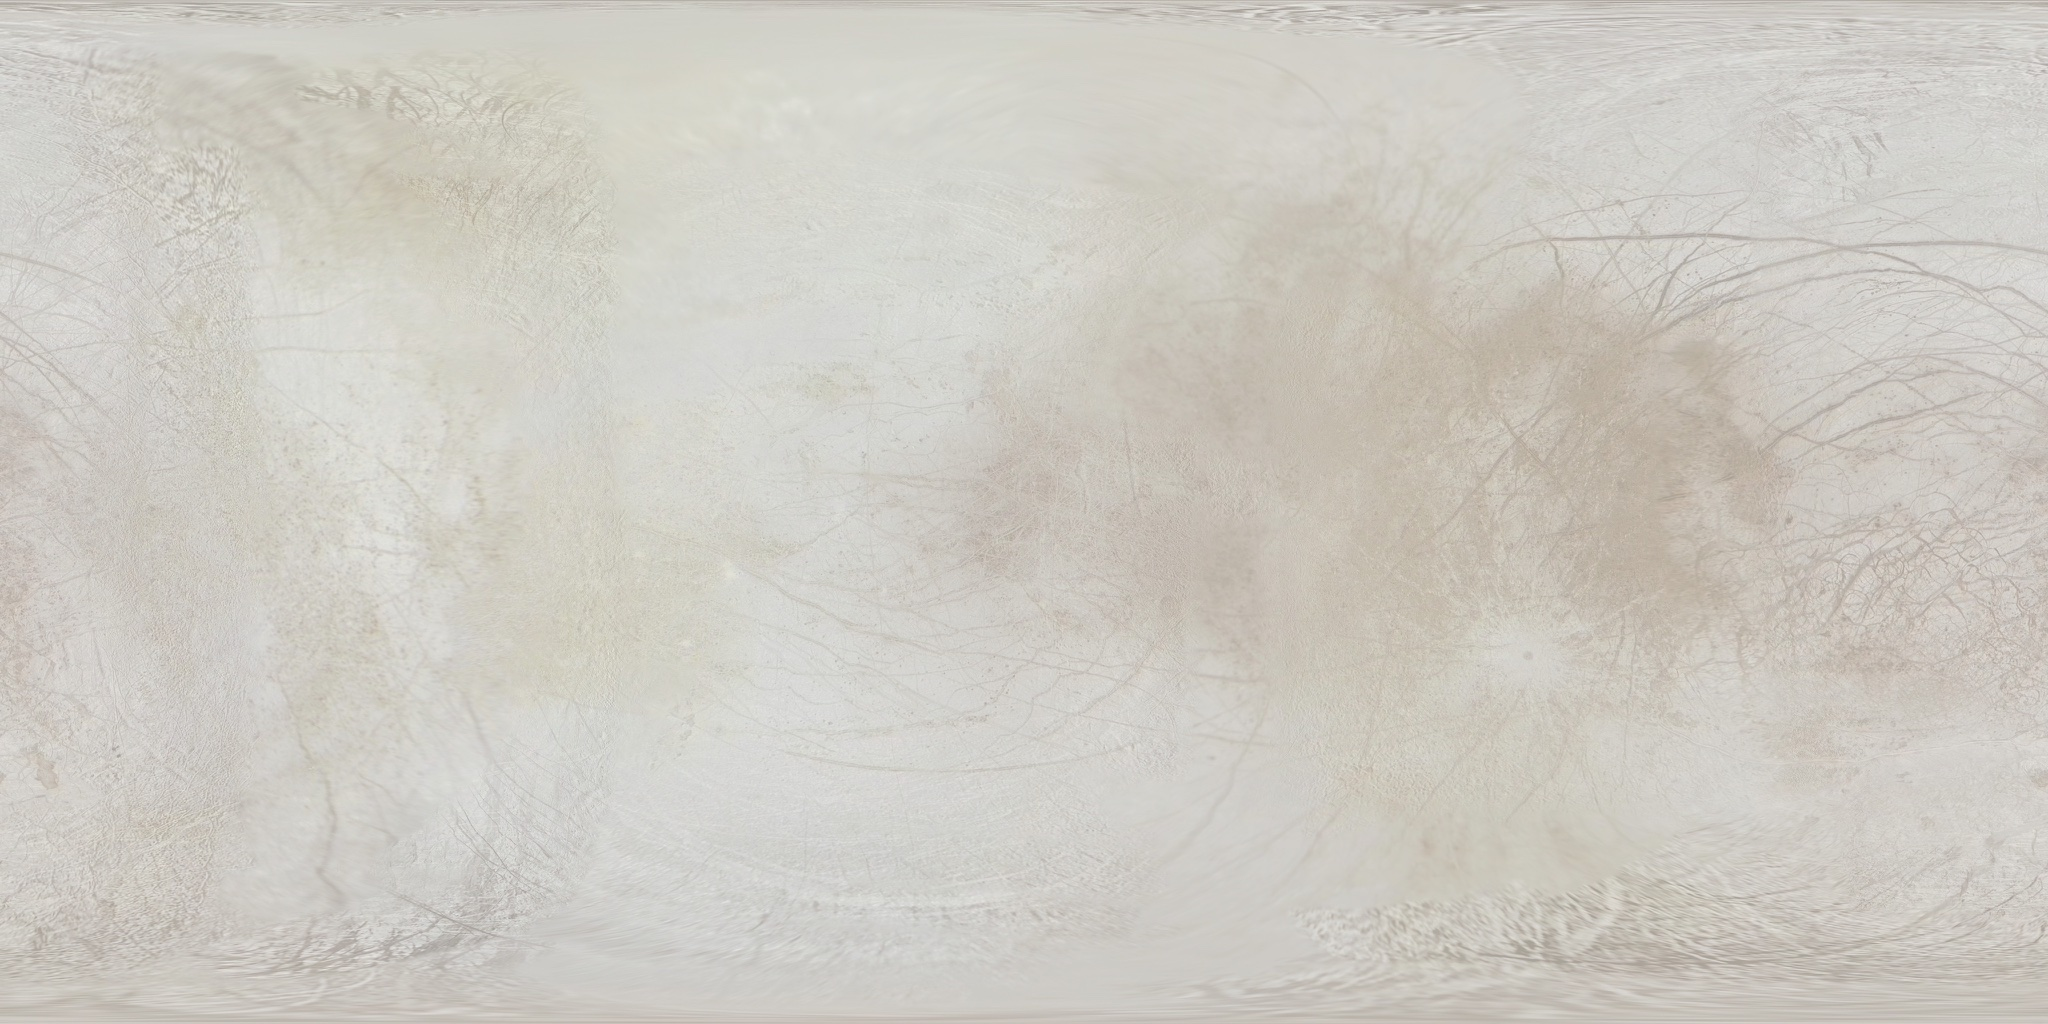
\includegraphics[width=\linewidth,height=4.4cm,keepaspectratio]{../public/textures/hd/europa_galileo.jpg}\\[2pt]
{\scriptsize\itshape\color{orbitarMuted} Planiglob desfășurat: Scoarța de gheață brăzdată de fracturi roșiatice (lineae) a lunii Europa, sub care se află un ocean global (NASA Galileo).}
\end{tabular}
\end{center}


\begin{tcolorbox}[orbitardata, title={\textbf{Repere esențiale: Europa}}]
\small
\begin{itemize}[leftmargin=1.4em, itemsep=2pt, topsep=2pt]
  \item \textbf{Clasificare și orbită:} Satelit Natural (Lună) (orbitează în jurul: \textbf{Jupiter}) \quad$\bullet$\quad \textbf{Distanță:} 5,204 UA ($\approx$ 779 milioane de kilometri)
  \item \textbf{Dimensiuni și masă:} rază medie 1.560,8 de kilometri \quad$\bullet$\quad masă: 0,008 $\times M_\oplus$
  \item \textbf{Gravitație și regim termic:} 0,134 $\times g_\oplus$ (1,31 m/s$^2$) \quad$\bullet$\quad temperatură medie: -160 $^\circ$C (înclinarea axei: Nespecificată)
  \item \textbf{Ciclu orbital și rotație:} perioadă orbitală (an): 3,551 zile pământești \quad$\bullet$\quad rotație (zi): 85,22 ore (3,55 zile pământești)
  \item \textbf{Durata călătoriei de pe Pământ:} cu viteza luminii ($1c$): \emph{35 de minute}; cu racheta ($50.000$ de kilometri pe oră): \emph{2,5--5 ani}; cu avionul ($900$ de kilometri pe oră): \emph{80 de ani}; cu mașina ($100$ de kilometri pe oră): \emph{717 ani}.
  \item \textbf{Repere de scară și curiozitate:} Europa este ca un ou de ciocolată cu surprize: tare și înghețată la exterior, dar cu un ocean adânc înăuntru! Deși Europa este mai mică decât Luna noastră, oceanul ei ascuns are de două ori mai multă apă decât toate oceanele Pământului!
\end{itemize}
\end{tcolorbox}

\subsubsection*{Prezentare generală și profil astrofizic}
Europa are cea mai netedă suprafață din Sistemul Solar, brăzdată de fracturi roșiatice numite \guillemotleft{}lineae\guillemotright{}. Sub crusta de gheață de 15--25 de kilometri grosime se află un ocean global de apă lichidă cu o adâncime estimată la 100 de kilometri, fiind unul dintre principalele locuri căutate pentru viață extraterestră. Europa este o lună acoperită cu un patinoar neted de gheață! Sub această coajă înghețată se ascunde un ocean uriaș de apă sărată. Europa este ca un ou de ciocolată cu surprize: tare și înghețată la exterior, dar cu un ocean adânc înăuntru!

\subsubsection*{Alcătuirea fizică și structura internă}
Privind în profunzimea sa, alcătuirea fizică este organizată pe mai multe straturi și regiuni distincte, fiecare având un rol bine definit în evoluția și dinamica acestui obiect cosmic. În primul rând se remarcă \textbf{Nucleu metalic și manta stâncoasă}, unde contactul direct dintre ocean și mantaua stâncoasă permite existența izvoarelor hidrotermale. În strânsă legătură cu această componentă se află \textbf{Ocean global subglaciar}, apă sărată menținută lichidă de încălzirea mareică joviană. În completarea acestui ansamblu întâlnim \textbf{Crustă activă de gheață}, plăci de gheață în mișcare și posibile gheizere de vapori de apă.

\subsubsection*{Observații astronomice și istoricul explorării}
Studiată de Galileo și Juno, fiind ținta principală a misiunilor JUICE (ESA) și Europa Clipper (NASA). Deși Europa este mai mică decât Luna noastră, oceanul ei ascuns are de două ori mai multă apă decât toate oceanele Pământului!

\vspace{6pt}
\begin{tcolorbox}[orbitarquiz, title={\textbf{Întrebare de verificare \#11: Europa}}]
\textbf{De ce sunt oamenii de știință atât de interesați de satelitul Europa?}
\begin{itemize}[leftmargin=2.2em, itemsep=2pt, topsep=4pt]
  \item[$\square$ \textbf{A.}] Are păduri tropicale
  \item[$\square$ \textbf{B.}] Adăpostește sub gheață un ocean global de apă lichidă care ar putea susține viață
  \item[$\square$ \textbf{C.}] Este cel mai fierbinte corp din Sistemul Solar
  \item[$\square$ \textbf{D.}] Are inele strălucitoare
\end{itemize}
\vspace{2pt}
{\footnotesize\color{orbitarMuted}\textbf{Răspuns corect:} \textbf{B} (Adăpostește sub gheață un ocean global de apă lichidă care ar putea susține viață). \emph{Oceanul subglaciar al Europei, aflat în contact cu un fund oceanic stâncos, oferă ingredientele esențiale pentru potențiale ecosisteme.}}
\end{tcolorbox}
\clearpage


\subsection{Ganymede}
\label{sec:body-ganymede}
\vspace{-4pt}
{\large\itshape\color{orbitarAccent} Cel mai mare satelit natural din Sistemul Solar}\\[4pt]


\begin{center}
\begin{tabular}{@{}m{0.44\textwidth}@{\hspace{0.03\textwidth}}m{0.51\textwidth}@{}}
\centering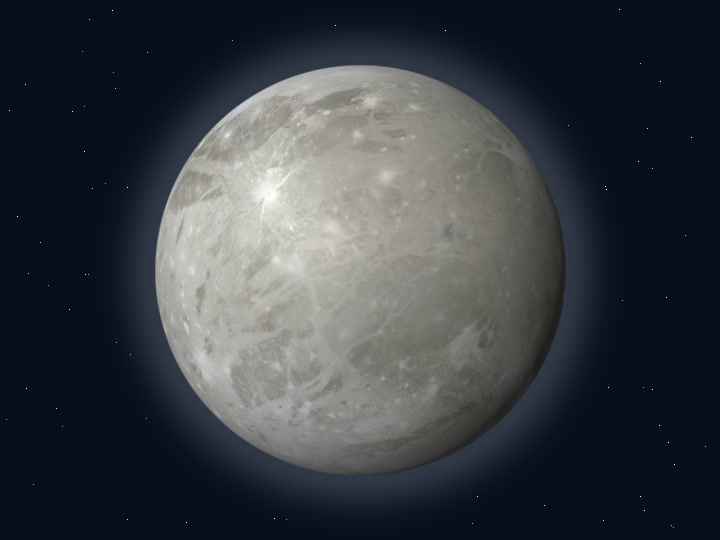
\includegraphics[width=\linewidth,height=4.4cm,keepaspectratio]{imagini/globuri/ganymede.jpg}\\[2pt]
{\scriptsize\itshape\color{orbitarMuted} Vedere 3D a corpului ceresc (\textbf{Ganymede})}
&
\centering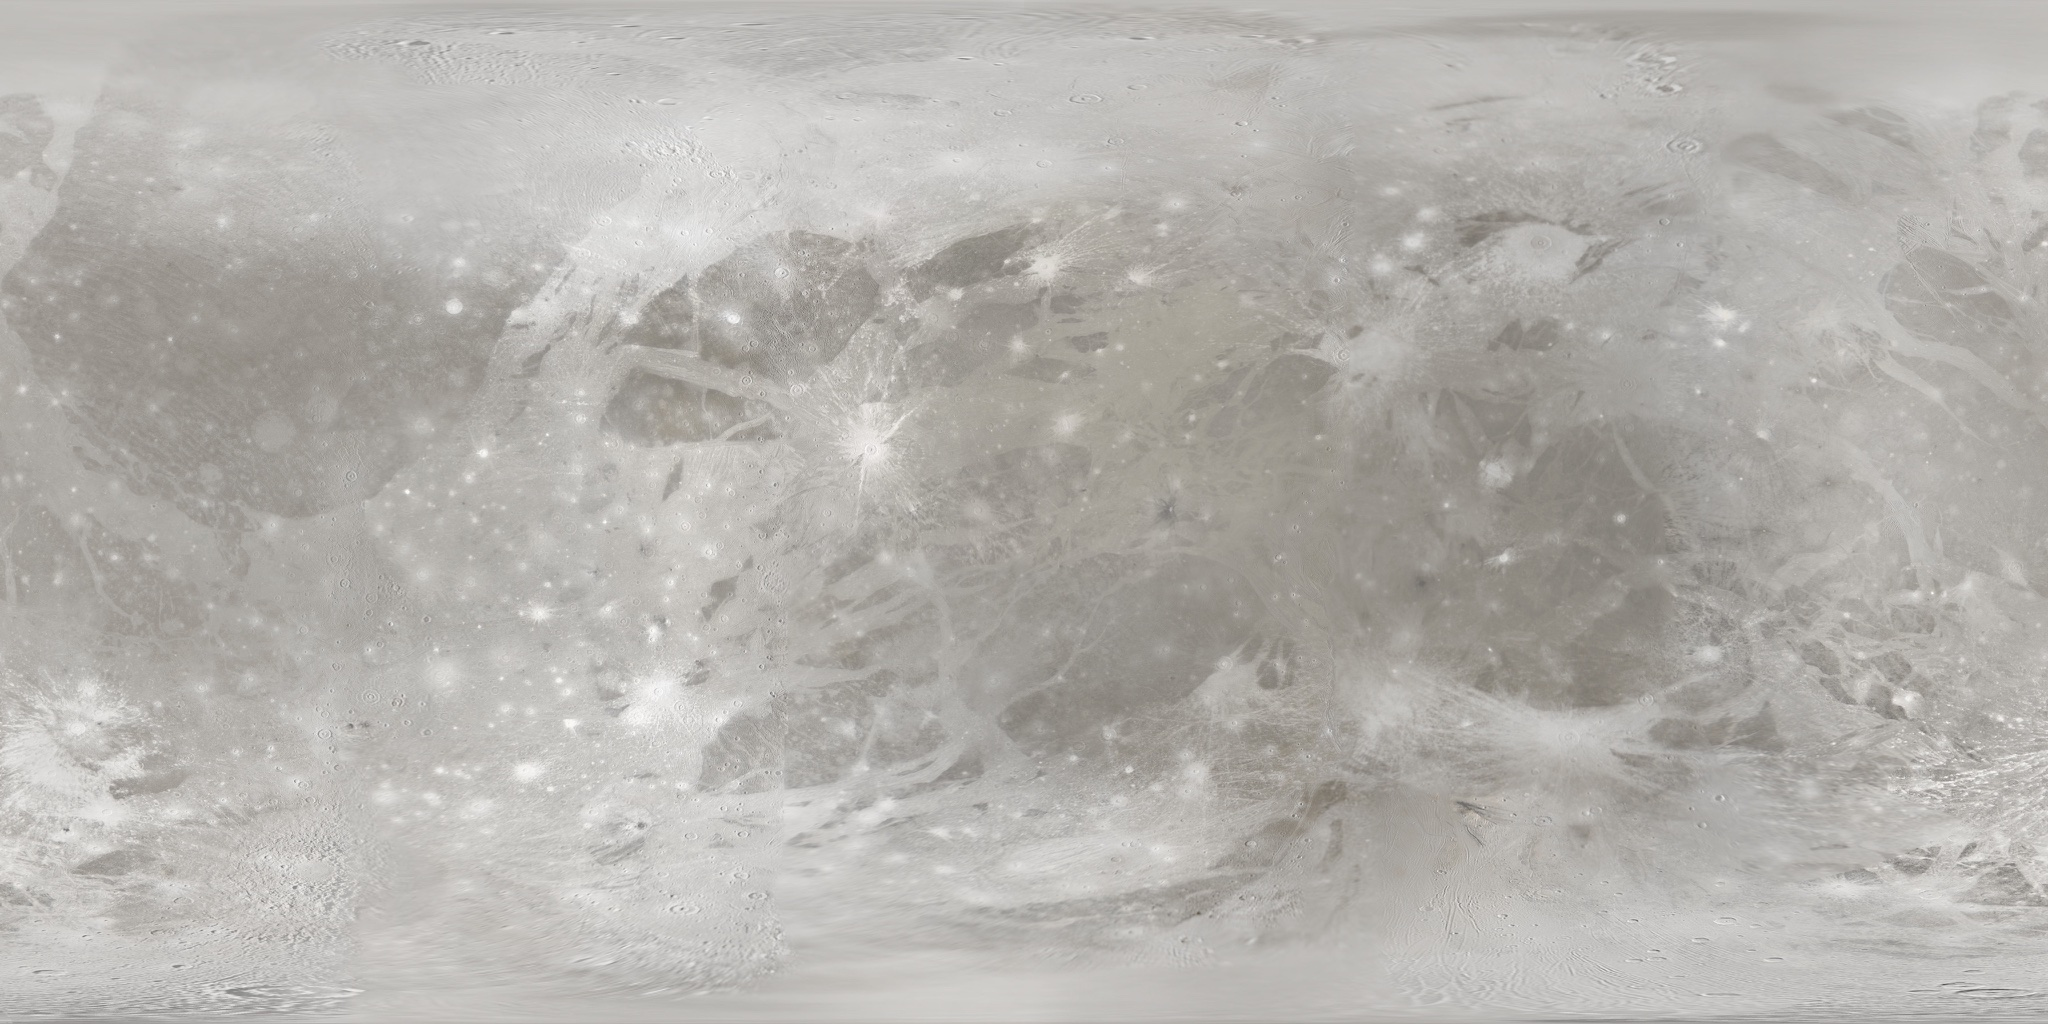
\includegraphics[width=\linewidth,height=4.4cm,keepaspectratio]{../public/textures/hd/ganymede_galileo.jpg}\\[2pt]
{\scriptsize\itshape\color{orbitarMuted} Planiglob desfășurat: Harta celui mai mare satelit din Sistemul Solar, Ganymede, obținută de misiunile NASA Voyager și Galileo.}
\end{tabular}
\end{center}


\begin{tcolorbox}[orbitardata, title={\textbf{Repere esențiale: Ganymede}}]
\small
\begin{itemize}[leftmargin=1.4em, itemsep=2pt, topsep=2pt]
  \item \textbf{Clasificare și orbită:} Satelit Natural (Lună) (orbitează în jurul: \textbf{Jupiter}) \quad$\bullet$\quad \textbf{Distanță:} 5,204 UA ($\approx$ 779 milioane de kilometri)
  \item \textbf{Dimensiuni și masă:} rază medie 2.631,2 de kilometri \quad$\bullet$\quad masă: 0,025 $\times M_\oplus$
  \item \textbf{Gravitație și regim termic:} 0,146 $\times g_\oplus$ (1,43 m/s$^2$) \quad$\bullet$\quad temperatură medie: -163 $^\circ$C (înclinarea axei: Nespecificată)
  \item \textbf{Ciclu orbital și rotație:} perioadă orbitală (an): 7,155 zile pământești \quad$\bullet$\quad rotație (zi): 171,70 ore (7,15 zile pământești)
  \item \textbf{Durata călătoriei de pe Pământ:} cu viteza luminii ($1c$): \emph{35 de minute}; cu racheta ($50.000$ de kilometri pe oră): \emph{2,5--5 ani}; cu avionul ($900$ de kilometri pe oră): \emph{80 de ani}; cu mașina ($100$ de kilometri pe oră): \emph{717 ani}.
  \item \textbf{Repere de scară și curiozitate:} Dacă Ganymede s-ar învârti direct în jurul Soarelui în loc de Jupiter, ar fi numită fără îndoială o planetă! Ganymede este singura lună din Sistemul Solar care are propriul ei scut magnetic și propriile aurore polare!
\end{itemize}
\end{tcolorbox}

\subsubsection*{Prezentare generală și profil astrofizic}
Cu un diametru de 5.262 de kilometri, Ganymede este cel mai mare satelit din Sistemul Solar și singurul cunoscut care posedă o magnetosferă intrinsecă, generată de convecția din nucleul său de fier lichid. Ganymede este campionul tuturor lunilor! Este atât de mare încât depășește chiar și planeta Mercur în dimensiune. Dacă Ganymede s-ar învârti direct în jurul Soarelui în loc de Jupiter, ar fi numită fără îndoială o planetă!

\subsubsection*{Alcătuirea fizică și structura internă}
Privind în profunzimea sa, alcătuirea fizică este organizată pe mai multe straturi și regiuni distincte, fiecare având un rol bine definit în evoluția și dinamica acestui obiect cosmic. În primul rând se remarcă \textbf{Nucleu de fier lichid}, care generează un câmp magnetic propriu în interiorul magnetosferei uriașe a lui Jupiter. În strânsă legătură cu această componentă se află \textbf{Straturi alternante de gheață și oceane}, unde modelele indică un ocean subteran uriaș prins între straturi de gheață de înaltă presiune. În completarea acestui ansamblu întâlnim \textbf{Scoarță mixtă}, regiuni întunecate străvechi craterizate și terenuri mai tinere, brăzdate de șanțuri tectonice.

\subsubsection*{Observații astronomice și istoricul explorării}
Descoperită în 1610 de Galileo Galilei; sonda europeană JUICE va deveni în 2034 prima navă care va intra pe orbita lui Ganymede. Ganymede este singura lună din Sistemul Solar care are propriul ei scut magnetic și propriile aurore polare!

\vspace{6pt}
\begin{tcolorbox}[orbitarquiz, title={\textbf{Întrebare de verificare \#12: Ganymede}}]
\textbf{Prin ce este Ganymede unic printre toți sateliții naturali din Sistemul Solar?}
\begin{itemize}[leftmargin=2.2em, itemsep=2pt, topsep=4pt]
  \item[$\square$ \textbf{A.}] Este cel mai mare satelit (mai mare decât Mercur) și are câmp magnetic propriu
  \item[$\square$ \textbf{B.}] Are vulcani de lavă fierbinte
  \item[$\square$ \textbf{C.}] Orbitează în jurul lui Marte
  \item[$\square$ \textbf{D.}] Este compus doar din gaz
\end{itemize}
\vspace{2pt}
{\footnotesize\color{orbitarMuted}\textbf{Răspuns corect:} \textbf{A} (Este cel mai mare satelit (mai mare decât Mercur) și are câmp magnetic propriu). \emph{Ganymede depășește în diametru planeta Mercur și este singurul satelit cu o magnetosferă proprie.}}
\end{tcolorbox}
\clearpage


\subsection{Callisto}
\label{sec:body-callisto}
\vspace{-4pt}
{\large\itshape\color{orbitarAccent} Lumea străveche de gheață și cratere a lui Jupiter}\\[4pt]


\begin{center}
\begin{tabular}{@{}m{0.44\textwidth}@{\hspace{0.03\textwidth}}m{0.51\textwidth}@{}}
\centering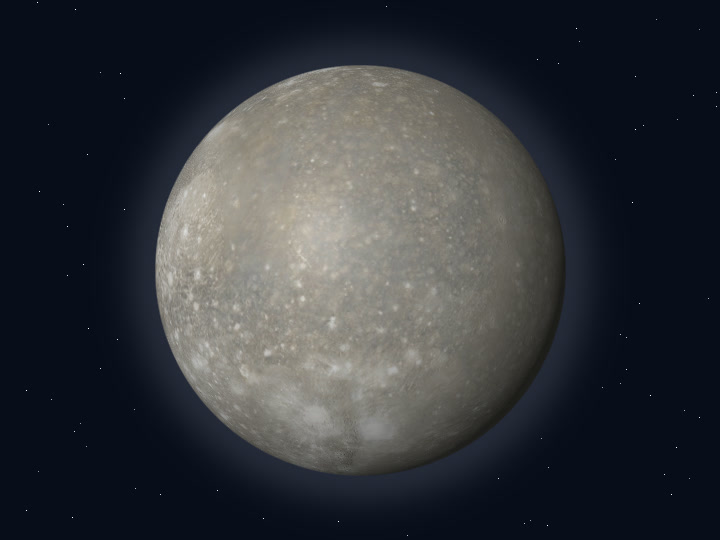
\includegraphics[width=\linewidth,height=4.4cm,keepaspectratio]{imagini/globuri/callisto.jpg}\\[2pt]
{\scriptsize\itshape\color{orbitarMuted} Vedere 3D a corpului ceresc (\textbf{Callisto})}
&
\centering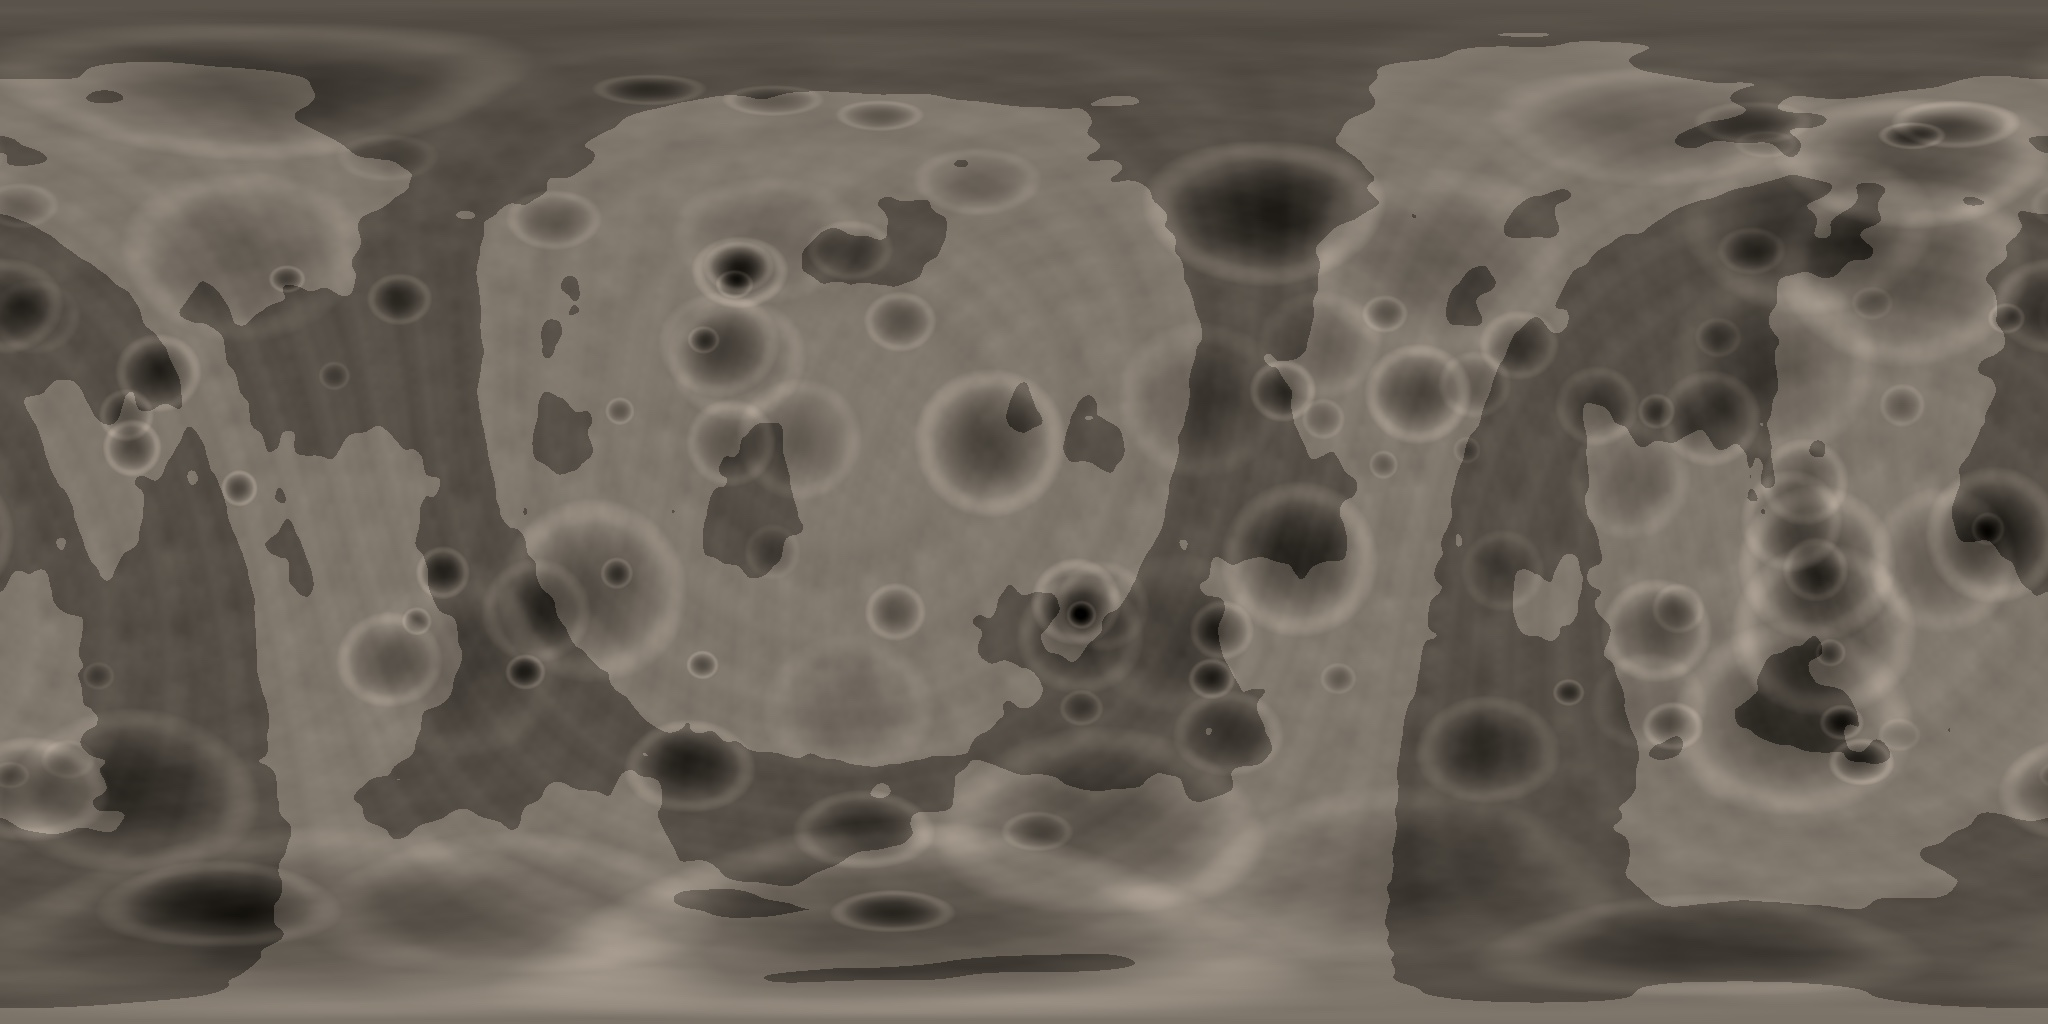
\includegraphics[width=\linewidth,height=4.4cm,keepaspectratio]{../public/textures/hd/callisto_galileo.jpg}\\[2pt]
{\scriptsize\itshape\color{orbitarMuted} Planiglob desfășurat: Suprafața străveche a lunii Callisto și bazinul multi-inelar Valhalla (date NASA Galileo).}
\end{tabular}
\end{center}


\begin{tcolorbox}[orbitardata, title={\textbf{Repere esențiale: Callisto}}]
\small
\begin{itemize}[leftmargin=1.4em, itemsep=2pt, topsep=2pt]
  \item \textbf{Clasificare și orbită:} Satelit Natural (Lună) (orbitează în jurul: \textbf{Jupiter}) \quad$\bullet$\quad \textbf{Distanță:} 5,204 UA ($\approx$ 779 milioane de kilometri)
  \item \textbf{Dimensiuni și masă:} rază medie 2.410,3 kilometri \quad$\bullet$\quad masă: 0,018 $\times M_\oplus$
  \item \textbf{Gravitație și regim termic:} 0,126 $\times g_\oplus$ (1,24 m/s$^2$) \quad$\bullet$\quad temperatură medie: -139 $^\circ$C (înclinarea axei: Nespecificată)
  \item \textbf{Ciclu orbital și rotație:} perioadă orbitală (an): 16,689 zile pământești \quad$\bullet$\quad rotație (zi): 400,50 ore (16,69 zile pământești)
  \item \textbf{Durata călătoriei de pe Pământ:} cu viteza luminii ($1c$): \emph{35 de minute}; cu racheta ($50.000$ de kilometri pe oră): \emph{2,5--5 ani}; cu avionul ($900$ de kilometri pe oră): \emph{80 de ani}; cu mașina ($100$ de kilometri pe oră): \emph{717 ani}.
  \item \textbf{Repere de scară și curiozitate:} Callisto arată ca un glob de Crăciun întunecat, presărat cu mii de scântei albe acolo unde au căzut meteoriți! Fiind mai departe de radiațiile puternice ale lui Jupiter, Callisto este locul preferat de ingineri pentru o viitoare bază umană!
\end{itemize}
\end{tcolorbox}

\subsubsection*{Prezentare generală și profil astrofizic}
Al treilea satelit ca mărime din Sistemul Solar (aproape cât Mercur) nu participă la rezonanța orbitală a celorlalte trei luni galileene, motiv pentru care nu a suferit încălzire mareică intensă, păstrând o arhivă geologică intactă de 4 miliarde de ani. Callisto este a patra lună mare a lui Jupiter și are cea mai veche suprafață din Sistemul Solar, plină de cratere strălucitoare de gheață! Callisto arată ca un glob de Crăciun întunecat, presărat cu mii de scântei albe acolo unde au căzut meteoriți!

\subsubsection*{Alcătuirea fizică și structura internă}
Privind în profunzimea sa, alcătuirea fizică este organizată pe mai multe straturi și regiuni distincte, fiecare având un rol bine definit în evoluția și dinamica acestui obiect cosmic. În primul rând se remarcă \textbf{Interior parțial diferențiat}, un amestec comprimat de rocă și gheață, fără un nucleu metalic mare complet separat. În strânsă legătură cu această componentă se află \textbf{Posibil ocean sărat la adâncime}, detectat indirect prin variațiile câmpului magnetic indus. În completarea acestui ansamblu întâlnim \textbf{Litosferă străveche}, dominată de Bazinul Valhalla, o structură de impact cu inele concentrice de 3.800 de kilometri diametru.

\subsubsection*{Observații astronomice și istoricul explorării}
Fotografiată în detaliu de Voyager 1/2 și Galileo; va fi survolată de 21 de ori de sonda JUICE. Fiind mai departe de radiațiile puternice ale lui Jupiter, Callisto este locul preferat de ingineri pentru o viitoare bază umană!

\vspace{6pt}
\begin{tcolorbox}[orbitarquiz, title={\textbf{Întrebare de verificare \#13: Callisto}}]
\textbf{Cum se numește uriașul bazin de impact cu inele concentrice de pe Callisto?}
\begin{itemize}[leftmargin=2.2em, itemsep=2pt, topsep=4pt]
  \item[$\square$ \textbf{A.}] Valhalla
  \item[$\square$ \textbf{B.}] Caloris
  \item[$\square$ \textbf{C.}] Olympus
  \item[$\square$ \textbf{D.}] Sputnik
\end{itemize}
\vspace{2pt}
{\footnotesize\color{orbitarMuted}\textbf{Răspuns corect:} \textbf{A} (Valhalla). \emph{Bazinul Valhalla este cel mai mare crater multi-inelar de pe Callisto, având un diametru de aproape 3.800 de kilometri.}}
\end{tcolorbox}
\clearpage


\section{Saturn}
\label{sec:body-saturn}
\vspace{-4pt}
{\large\itshape\color{orbitarAccent} Bijuteria Sistemului Solar, încoronată cu inele de gheață}\\[4pt]


\begin{center}
\begin{tabular}{@{}m{0.44\textwidth}@{\hspace{0.03\textwidth}}m{0.51\textwidth}@{}}
\centering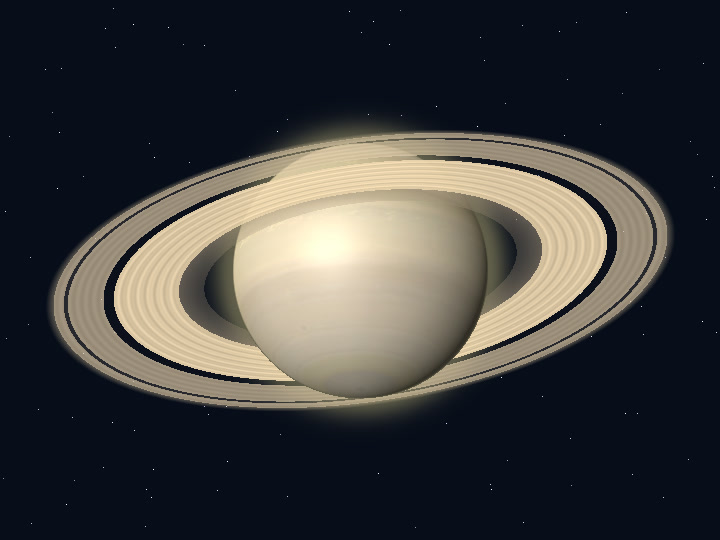
\includegraphics[width=\linewidth,height=4.4cm,keepaspectratio]{imagini/globuri/saturn.jpg}\\[2pt]
{\scriptsize\itshape\color{orbitarMuted} Vedere 3D a corpului ceresc (\textbf{Saturn})}
&
\centering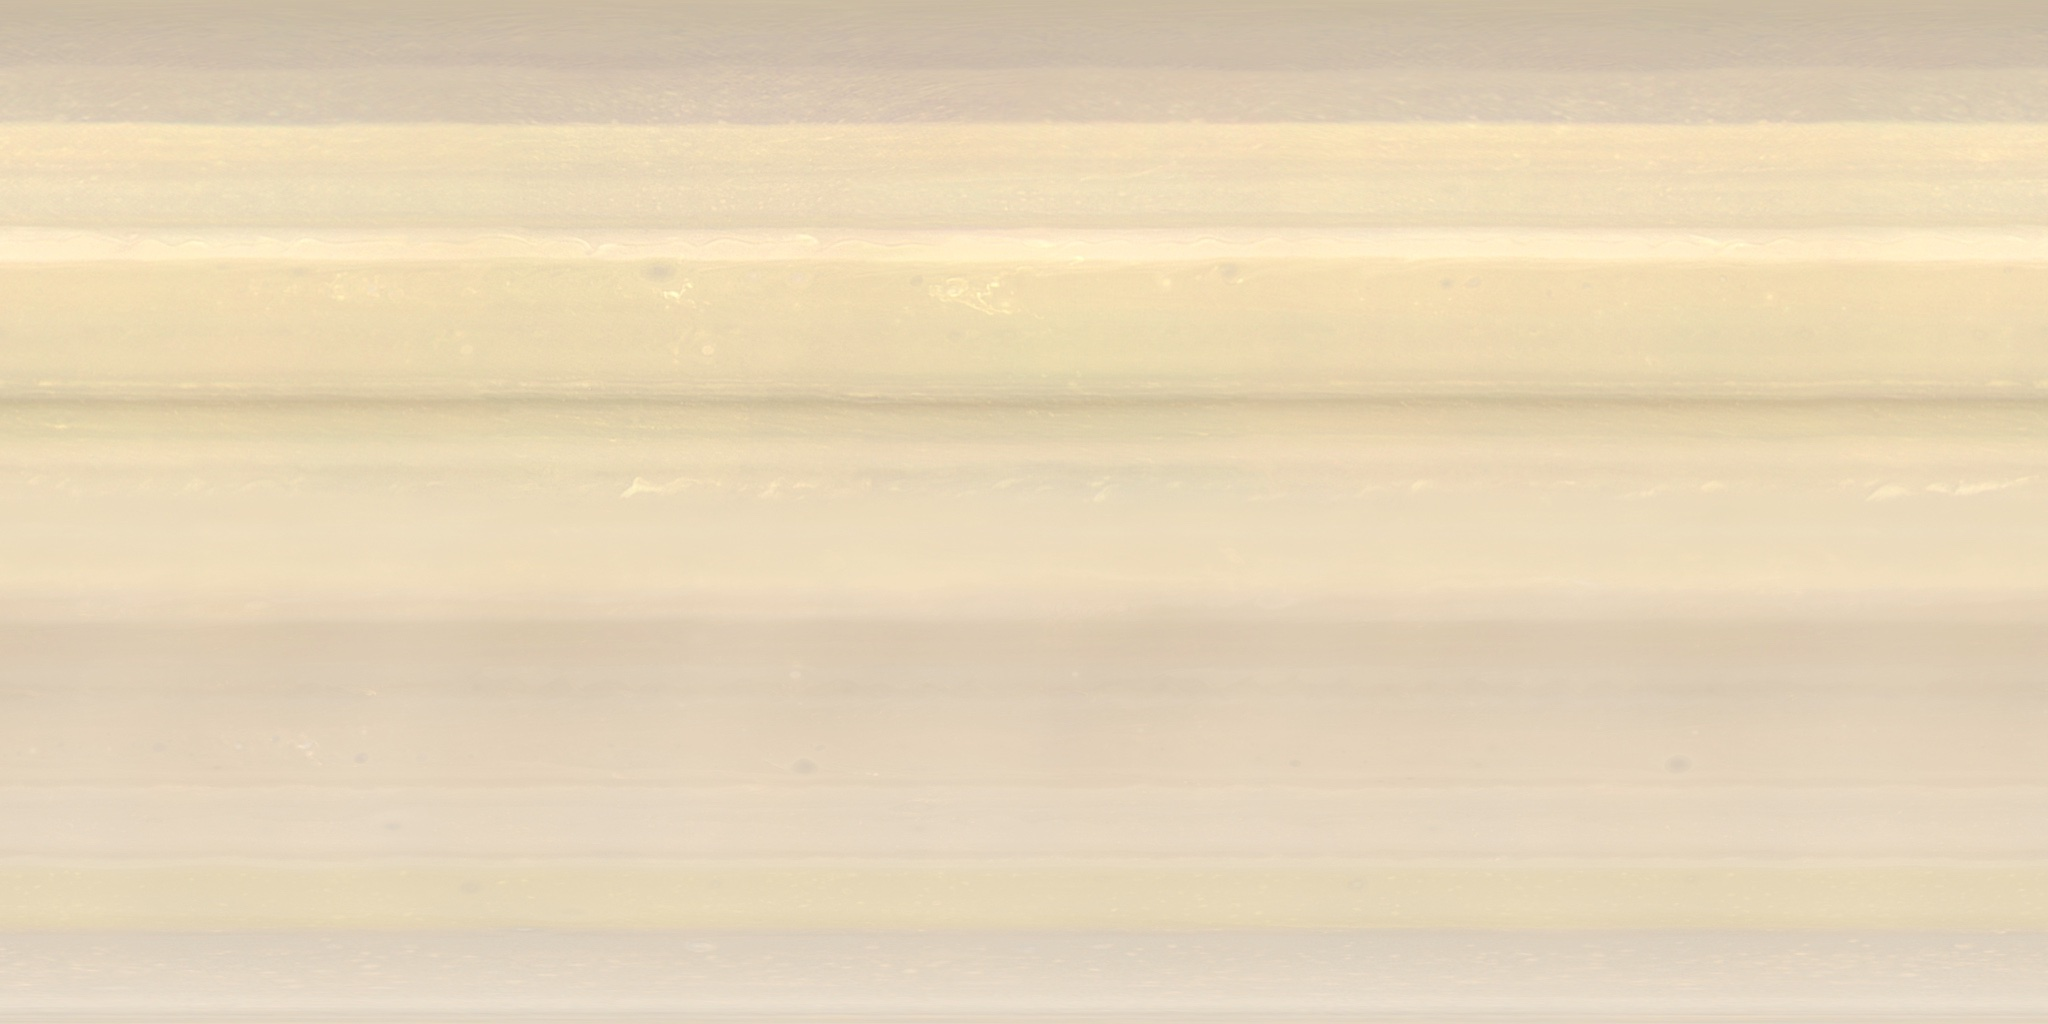
\includegraphics[width=\linewidth,height=4.4cm,keepaspectratio]{../public/textures/hd/saturn_cassini_albedo.jpg}\\[2pt]
{\scriptsize\itshape\color{orbitarMuted} Planiglob desfășurat: Harta benzilor atmosferice aurii ale gigantului gazos Saturn (date NASA/ESA Cassini).}
\end{tabular}
\end{center}


\begin{tcolorbox}[orbitardata, title={\textbf{Repere esențiale: Saturn}}]
\small
\begin{itemize}[leftmargin=1.4em, itemsep=2pt, topsep=2pt]
  \item \textbf{Clasificare și orbită:} Gigant Gazos \quad$\bullet$\quad \textbf{Distanță:} 9,582 UA ($\approx$ 1.433 milioane de kilometri)
  \item \textbf{Dimensiuni și masă:} rază medie 58.232 de kilometri \quad$\bullet$\quad masă: 95,160 $\times M_\oplus$
  \item \textbf{Gravitație și regim termic:} 1,060 $\times g_\oplus$ (10,40 m/s$^2$) \quad$\bullet$\quad temperatură medie: -140 $^\circ$C (înclinarea axei: 26,73$^\circ$)
  \item \textbf{Ciclu orbital și rotație:} perioadă orbitală (an): 10.759,22 zile ($\approx$ 29,46 ani pământești) \quad$\bullet$\quad rotație (zi): 10,70 ore (0,45 zile pământești)
  \item \textbf{Durata călătoriei de pe Pământ:} cu viteza luminii ($1c$): \emph{1 oră și 11 minute}; cu racheta ($50.000$ de kilometri pe oră): \emph{3 până la 7 ani}; cu avionul ($900$ de kilometri pe oră): \emph{160 de ani}; cu mașina ($100$ de kilometri pe oră): \emph{1.450 de ani}.
  \item \textbf{Repere de scară și curiozitate:} Saturn este atât de ușor pentru mărimea lui încât, dacă am avea o cadă cu apă destul de mare, planeta ar pluti! La polul nord al lui Saturn există un vârtej de nori cu o formă geometrică perfectă de hexagon!
\end{itemize}
\end{tcolorbox}

\subsubsection*{Prezentare generală și profil astrofizic}
Al doilea gigant gazos ca mărime are o densitate medie de doar 0,687 g/cm$^3$ (mai mică decât a apei). Sistemul său principal de inele (A, B, C) are o lățime de 282.000 de kilometri, dar o grosime medie de numai 10--30 de metri. Saturn este cea mai ușor de recunoscut planetă datorită inelelor sale strălucitoare! Aceste inele sunt făcute din miliarde de bulgări de gheață și praf cosmic. Saturn este atât de ușor pentru mărimea lui încât, dacă am avea o cadă cu apă destul de mare, planeta ar pluti!

\subsubsection*{Alcătuirea fizică și structura internă}
Privind în profunzimea sa, alcătuirea fizică este organizată pe mai multe straturi și regiuni distincte, fiecare având un rol bine definit în evoluția și dinamica acestui obiect cosmic. În primul rând se remarcă \textbf{Nucleu dens stâncos-metalic}, de 9--22 de ori masa Pământului, înconjurat de hidrogen metalic lichid. În strânsă legătură cu această componentă se află \textbf{Atmosferă aurie cu vânturi de 1.800 kilometri pe oră}, dominată de hidrogen și heliu, cu un jet-stream hexagonal persistent la polul nord. În completarea acestui ansamblu întâlnim \textbf{Sistemul de Inele}, compus 99\% din gheață pură de apă, cu dimensiuni de la granule microscopice la blocuri de câțiva metri.

\subsubsection*{Observații astronomice și istoricul explorării}
Vizitată de Pioneer 11 și Voyager 1/2, apoi explorată în detaliu timp de 13 ani de misiunea istorică Cassini-Huygens (2004--2017). La polul nord al lui Saturn există un vârtej de nori cu o formă geometrică perfectă de hexagon!

\vspace{6pt}
\begin{tcolorbox}[orbitarquiz, title={\textbf{Întrebare de verificare \#14: Saturn}}]
\textbf{Din ce sunt alcătuite în principal celebrele inele ale lui Saturn?}
\begin{itemize}[leftmargin=2.2em, itemsep=2pt, topsep=4pt]
  \item[$\square$ \textbf{A.}] Din inele solide de metal
  \item[$\square$ \textbf{B.}] Din gaze colorate
  \item[$\square$ \textbf{C.}] Din miliarde de fragmente de gheață și rocă
  \item[$\square$ \textbf{D.}] Din lavă vulcanică înghețată
\end{itemize}
\vspace{2pt}
{\footnotesize\color{orbitarMuted}\textbf{Răspuns corect:} \textbf{C} (Din miliarde de fragmente de gheață și rocă). \emph{Inelele lui Saturn nu sunt solide, ci sunt formate din nenumărate particule și blocuri de gheață care orbitează independent planeta.}}
\end{tcolorbox}
\clearpage


\subsection{Mimas}
\label{sec:body-mimas}
\vspace{-4pt}
{\large\itshape\color{orbitarAccent} Luna înghețată a lui Saturn cu craterul gigant Herschel}\\[4pt]


\begin{center}
\begin{tabular}{@{}m{0.44\textwidth}@{\hspace{0.03\textwidth}}m{0.51\textwidth}@{}}
\centering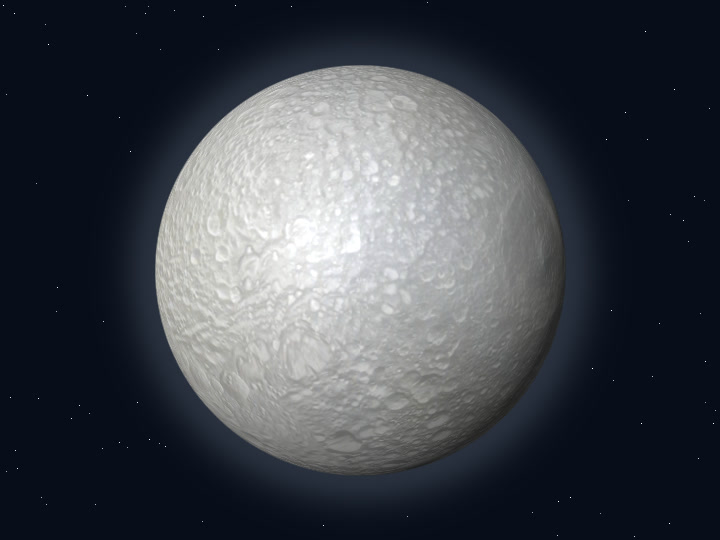
\includegraphics[width=\linewidth,height=4.4cm,keepaspectratio]{imagini/globuri/mimas.jpg}\\[2pt]
{\scriptsize\itshape\color{orbitarMuted} Vedere 3D a corpului ceresc (\textbf{Mimas})}
&
\centering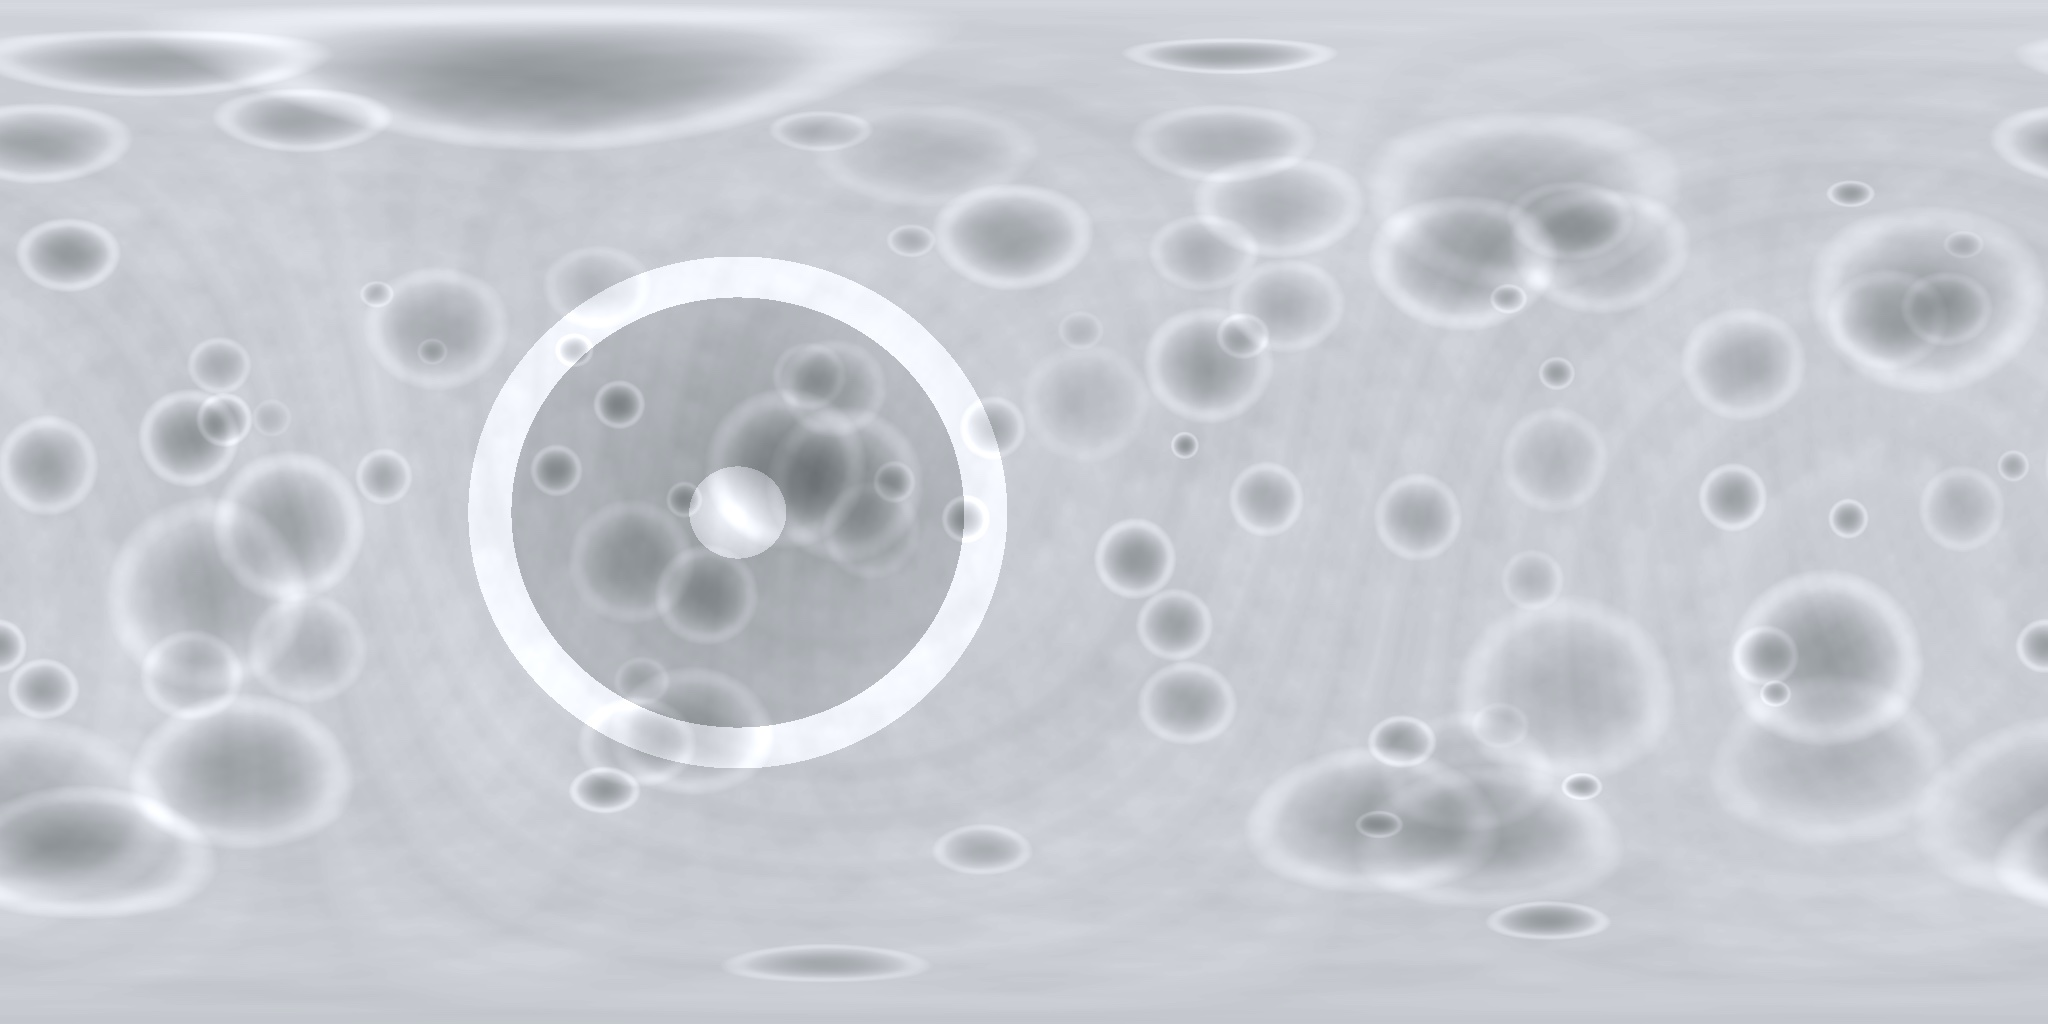
\includegraphics[width=\linewidth,height=4.4cm,keepaspectratio]{../public/textures/hd/mimas_cassini.jpg}\\[2pt]
{\scriptsize\itshape\color{orbitarMuted} Planiglob desfășurat: Harta satelitul înghețat Mimas și a uriașului crater Herschel, fotografiate de sonda NASA/ESA Cassini.}
\end{tabular}
\end{center}


\begin{tcolorbox}[orbitardata, title={\textbf{Repere esențiale: Mimas}}]
\small
\begin{itemize}[leftmargin=1.4em, itemsep=2pt, topsep=2pt]
  \item \textbf{Clasificare și orbită:} Satelit Natural (Lună) (orbitează în jurul: \textbf{Saturn}) \quad$\bullet$\quad \textbf{Distanță:} 9,582 UA ($\approx$ 1.433 milioane de kilometri)
  \item \textbf{Dimensiuni și masă:} rază medie 198,2 de kilometri \quad$\bullet$\quad masă: 6,30e-6 $\times M_\oplus$
  \item \textbf{Gravitație și regim termic:} 0,006 $\times g_\oplus$ (0,06 m/s$^2$) \quad$\bullet$\quad temperatură medie: -209 $^\circ$C (înclinarea axei: Nespecificată)
  \item \textbf{Ciclu orbital și rotație:} perioadă orbitală (an): 0,942 zile pământești \quad$\bullet$\quad rotație (zi): 22,61 ore (0,94 zile pământești)
  \item \textbf{Durata călătoriei de pe Pământ:} cu viteza luminii ($1c$): \emph{1 oră și 11 minute}; cu racheta ($50.000$ de kilometri pe oră): \emph{7 ani}; cu avionul ($900$ de kilometri pe oră): \emph{160 de ani}; cu mașina ($100$ de kilometri pe oră): \emph{1.450 de ani}.
  \item \textbf{Repere de scară și curiozitate:} Mimas este cel mai mic corp ceresc din Sistemul Solar care a reușit să devină rotund sub propria lui gravitație! Deși la exterior arată ca un glob înghețat și nemișcat, sub gheața lui Mimas se ascunde un ocean tânăr de apă lichidă!
\end{itemize}
\end{tcolorbox}

\subsubsection*{Prezentare generală și profil astrofizic}
Descoperită în 1789 de William Herschel, Mimas orbitează Saturn în doar 22 de ore și 36 de minute și curăță gravitațional celebra Diviziune Cassini dintre inelele A și B. Craterul Herschel are 139 de kilometri în diametru, ceea ce reprezintă o treime din diametrul întregului satelit! Mimas este o lună mică și înghețată a lui Saturn, celebră pentru craterul ei uriaș numit Herschel, care o face să arate exact ca o navă spațială din filme! Mimas este cel mai mic corp ceresc din Sistemul Solar care a reușit să devină rotund sub propria lui gravitație!

\subsubsection*{Alcătuirea fizică și structura internă}
Privind în profunzimea sa, alcătuirea fizică este organizată pe mai multe straturi și regiuni distincte, fiecare având un rol bine definit în evoluția și dinamica acestui obiect cosmic. În primul rând se remarcă \textbf{Nucleu stâncos}, înconjurat de un ocean global tânăr (format acum 5--15 milioane de ani), confirmat în 2024 din analiza librațiilor sondei Cassini. În strânsă legătură cu această componentă se află \textbf{Carapace groasă de gheață (20--30 de kilometri)}, atât de groasă încât nu prezintă gheizere la suprafață, spre deosebire de vecina Enceladus. În completarea acestui ansamblu întâlnim \textbf{Craterul Herschel}, ziduri de 5 kilometri înălțime și un piscul central de 6 kilometri, rezultat dintr-un impact la limita dezintegrării satelitului.

\subsubsection*{Observații astronomice și istoricul explorării}
Fotografiată de Voyager 1/2 și cartografiată la înaltă rezoluție de sonda Cassini între 2004 și 2017. Deși la exterior arată ca un glob înghețat și nemișcat, sub gheața lui Mimas se ascunde un ocean tânăr de apă lichidă!

\vspace{6pt}
\begin{tcolorbox}[orbitarquiz, title={\textbf{Întrebare de verificare \#15: Mimas}}]
\textbf{Ce formațiune geologică celebră ocupă o treime din diametrul satelitului Mimas?}
\begin{itemize}[leftmargin=2.2em, itemsep=2pt, topsep=4pt]
  \item[$\square$ \textbf{A.}] Craterul Herschel
  \item[$\square$ \textbf{B.}] Vulcanul Olympus Mons
  \item[$\square$ \textbf{C.}] Canionul Valles Marineris
  \item[$\square$ \textbf{D.}] Marea Tranquillitatis
\end{itemize}
\vspace{2pt}
{\footnotesize\color{orbitarMuted}\textbf{Răspuns corect:} \textbf{A} (Craterul Herschel). \emph{Craterul Herschel are 139 de kilometri lățime și un munte central înalt de 6 kilometri, dându-i lui Mimas aspectul său inconfundabil.}}
\end{tcolorbox}
\clearpage


\subsection{Enceladus}
\label{sec:body-enceladus}
\vspace{-4pt}
{\large\itshape\color{orbitarAccent} Luna albă ca zăpada a lui Saturn, cu gheizere cosmice}\\[4pt]


\begin{center}
\begin{tabular}{@{}m{0.44\textwidth}@{\hspace{0.03\textwidth}}m{0.51\textwidth}@{}}
\centering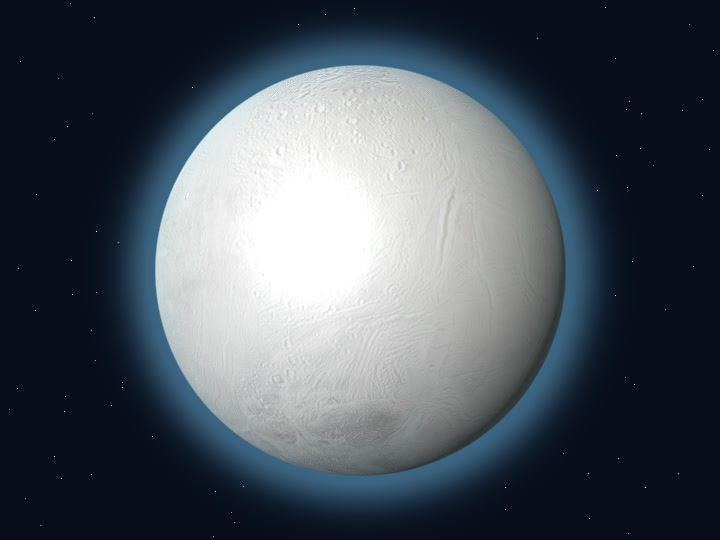
\includegraphics[width=\linewidth,height=4.4cm,keepaspectratio]{imagini/globuri/enceladus.jpg}\\[2pt]
{\scriptsize\itshape\color{orbitarMuted} Vedere 3D a corpului ceresc (\textbf{Enceladus})}
&
\centering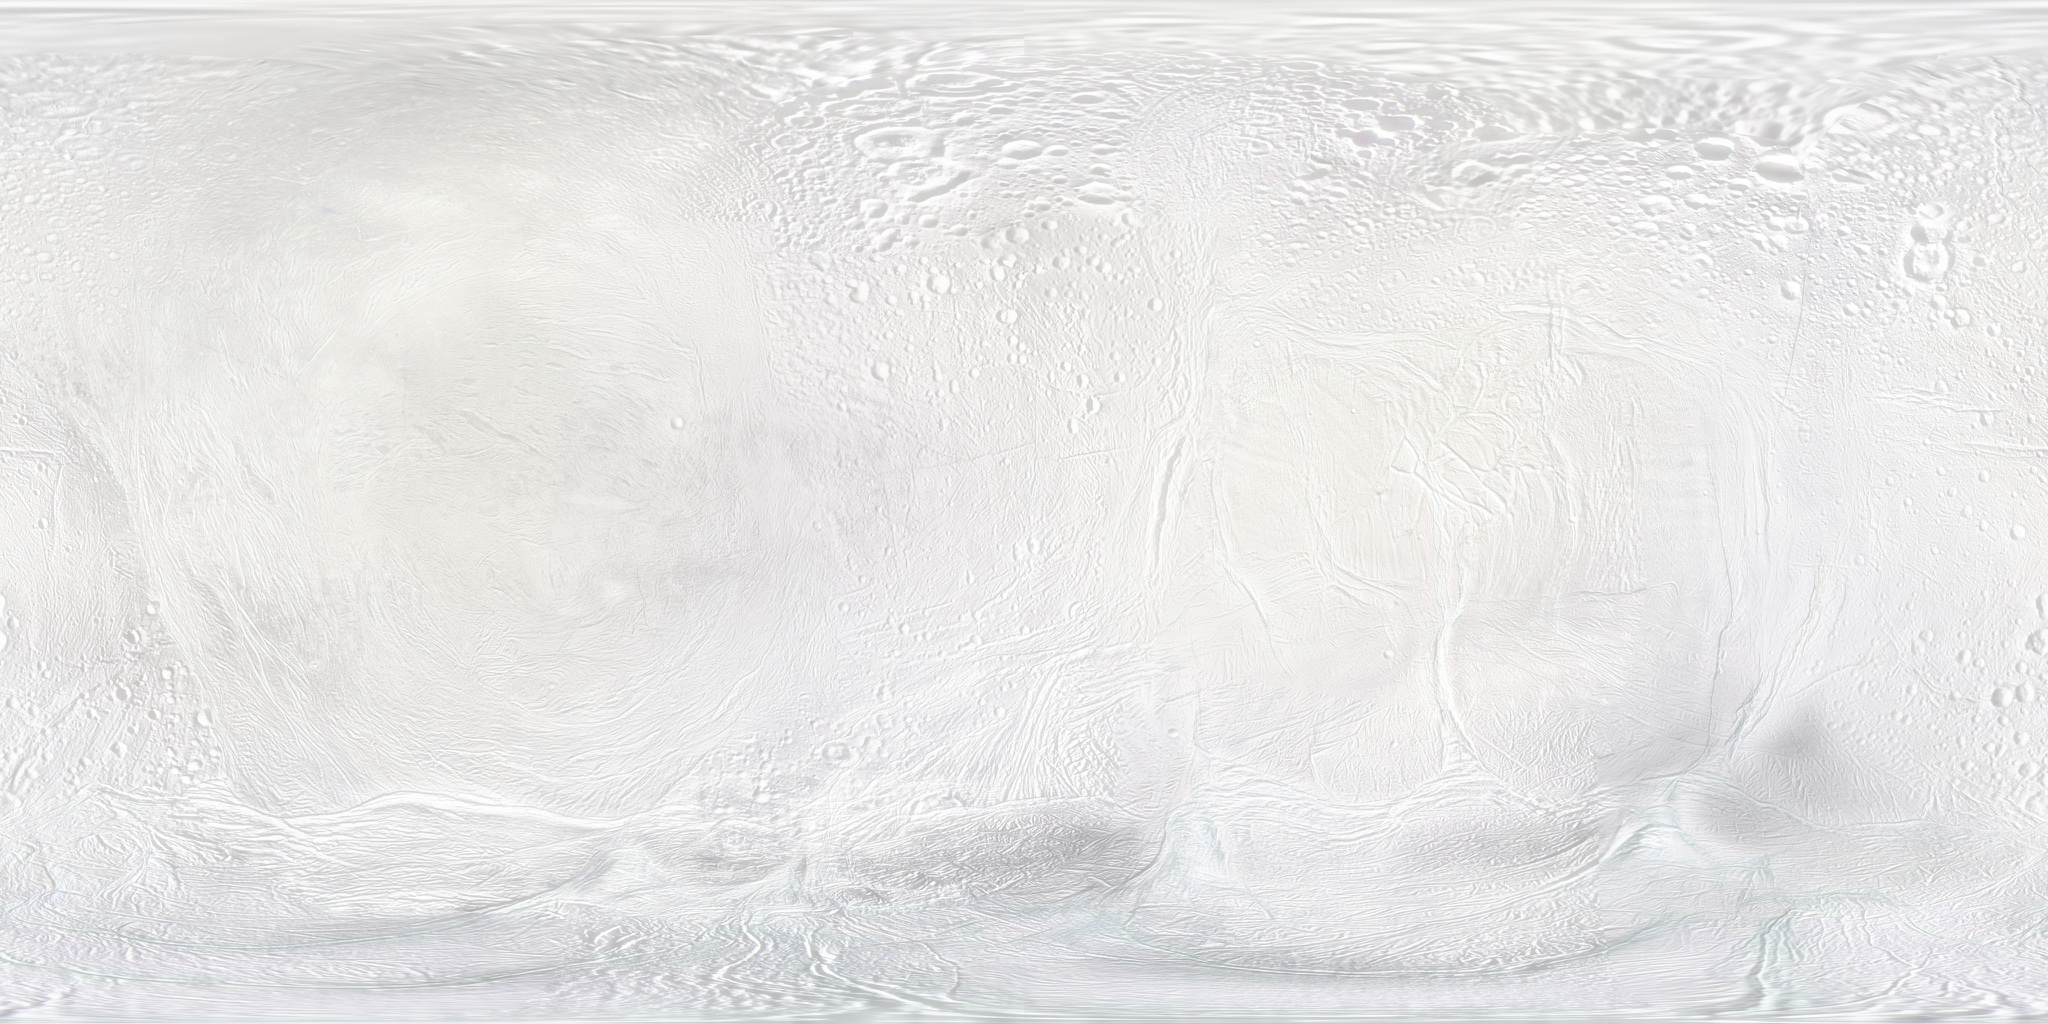
\includegraphics[width=\linewidth,height=4.4cm,keepaspectratio]{../public/textures/hd/enceladus_cassini.jpg}\\[2pt]
{\scriptsize\itshape\color{orbitarMuted} Planiglob desfășurat: Gheața pură a lunii Enceladus și fisurile \quotedblbase{}Dungi de Tigru\textquotedblright{} de la polul sudic (sonda NASA/ESA Cassini).}
\end{tabular}
\end{center}


\begin{tcolorbox}[orbitardata, title={\textbf{Repere esențiale: Enceladus}}]
\small
\begin{itemize}[leftmargin=1.4em, itemsep=2pt, topsep=2pt]
  \item \textbf{Clasificare și orbită:} Satelit Natural (Lună) (orbitează în jurul: \textbf{Saturn}) \quad$\bullet$\quad \textbf{Distanță:} 9,582 UA ($\approx$ 1.433 milioane de kilometri)
  \item \textbf{Dimensiuni și masă:} rază medie 252,1 de kilometri \quad$\bullet$\quad masă: 1,80e-5 $\times M_\oplus$
  \item \textbf{Gravitație și regim termic:} 0,011 $\times g_\oplus$ (0,11 m/s$^2$) \quad$\bullet$\quad temperatură medie: -198 $^\circ$C (înclinarea axei: Nespecificată)
  \item \textbf{Ciclu orbital și rotație:} perioadă orbitală (an): 1,37 zile pământești \quad$\bullet$\quad rotație (zi): 32,88 ore (1,37 zile pământești)
  \item \textbf{Durata călătoriei de pe Pământ:} cu viteza luminii ($1c$): \emph{1 oră și 11 minute}; cu racheta ($50.000$ de kilometri pe oră): \emph{7 ani}; cu avionul ($900$ de kilometri pe oră): \emph{160 de ani}; cu mașina ($100$ de kilometri pe oră): \emph{1.450 de ani}.
  \item \textbf{Repere de scară și curiozitate:} Enceladus este atât de mic încât ar încăpea cu ușurință deasupra României! Cristalele de gheață aruncate de gheizerele lui Enceladus formează unul dintre inelele lui Saturn (inelul E)!
\end{itemize}
\end{tcolorbox}

\subsubsection*{Prezentare generală și profil astrofizic}
Enceladus are cel mai ridicat albedo (reflectivitate) din Sistemul Solar (aproximativ 0,99). Sonda Cassini a zburat direct prin jeturile sale criovulcanice de la polul sud (\guillemotleft{}Dungile de Tigru\guillemotright{}), detectând apă sărată, molecule organice complexe, hidrogen molecular și silice hidrotermală. Enceladus este un bulgăre strălucitor de gheață proaspătă! La polul său sudic, gheizere uriașe aruncă apă și cristale de gheață direct în spațiu. Enceladus este atât de mic încât ar încăpea cu ușurință deasupra României!

\subsubsection*{Alcătuirea fizică și structura internă}
Privind în profunzimea sa, alcătuirea fizică este organizată pe mai multe straturi și regiuni distincte, fiecare având un rol bine definit în evoluția și dinamica acestui obiect cosmic. În primul rând se remarcă \textbf{Nucleu poros stâncos}, încălzit de mareele lui Saturn, generează izvoare hidrotermale pe fundul oceanului. În strânsă legătură cu această componentă se află \textbf{Ocean global subglaciar}, strat de apă lichidă de 30--40 de kilometri adâncime sub calota de gheață. În completarea acestui ansamblu întâlnim \textbf{Crustă de gheață pură și fisuri criovulcanice}, patru fracturi paralele calde la polul sudic prin care iese apa oceanică în vid.

\subsubsection*{Observații astronomice și istoricul explorării}
Descoperită de William Herschel în 1789; gheizerele sale au fost descoperite și analizate chimic de sonda Cassini în 2005--2015. Cristalele de gheață aruncate de gheizerele lui Enceladus formează unul dintre inelele lui Saturn (inelul E)!

\vspace{6pt}
\begin{tcolorbox}[orbitarquiz, title={\textbf{Întrebare de verificare \#16: Enceladus}}]
\textbf{Ce alimentează inelul E al planetei Saturn?}
\begin{itemize}[leftmargin=2.2em, itemsep=2pt, topsep=4pt]
  \item[$\square$ \textbf{A.}] Praf de pe Marte
  \item[$\square$ \textbf{B.}] Gheizerele de gheață și vapori de apă de la polul sud al lui Enceladus
  \item[$\square$ \textbf{C.}] Vântul solar
  \item[$\square$ \textbf{D.}] Asteroizii din Centura Kuiper
\end{itemize}
\vspace{2pt}
{\footnotesize\color{orbitarMuted}\textbf{Răspuns corect:} \textbf{B} (Gheizerele de gheață și vapori de apă de la polul sud al lui Enceladus). \emph{Jetul criovulcanic al lui Enceladus expulzează continuu granule de gheață care scapă de gravitația micului satelit și formează inelul E.}}
\end{tcolorbox}
\clearpage


\subsection{Tethys}
\label{sec:body-tethys}
\vspace{-4pt}
{\large\itshape\color{orbitarAccent} Luna de gheață pură a lui Saturn, cu craterul Odysseus și canionul Ithaca}\\[4pt]


\begin{center}
\begin{tabular}{@{}m{0.44\textwidth}@{\hspace{0.03\textwidth}}m{0.51\textwidth}@{}}
\centering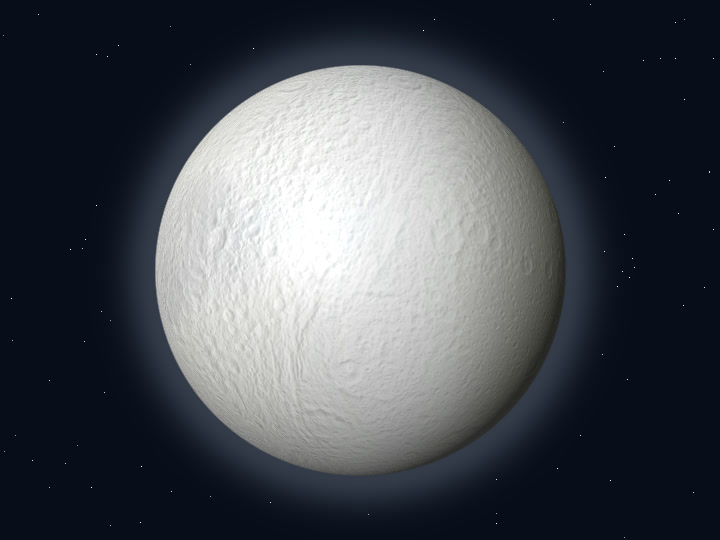
\includegraphics[width=\linewidth,height=4.4cm,keepaspectratio]{imagini/globuri/tethys.jpg}\\[2pt]
{\scriptsize\itshape\color{orbitarMuted} Vedere 3D a corpului ceresc (\textbf{Tethys})}
&
\centering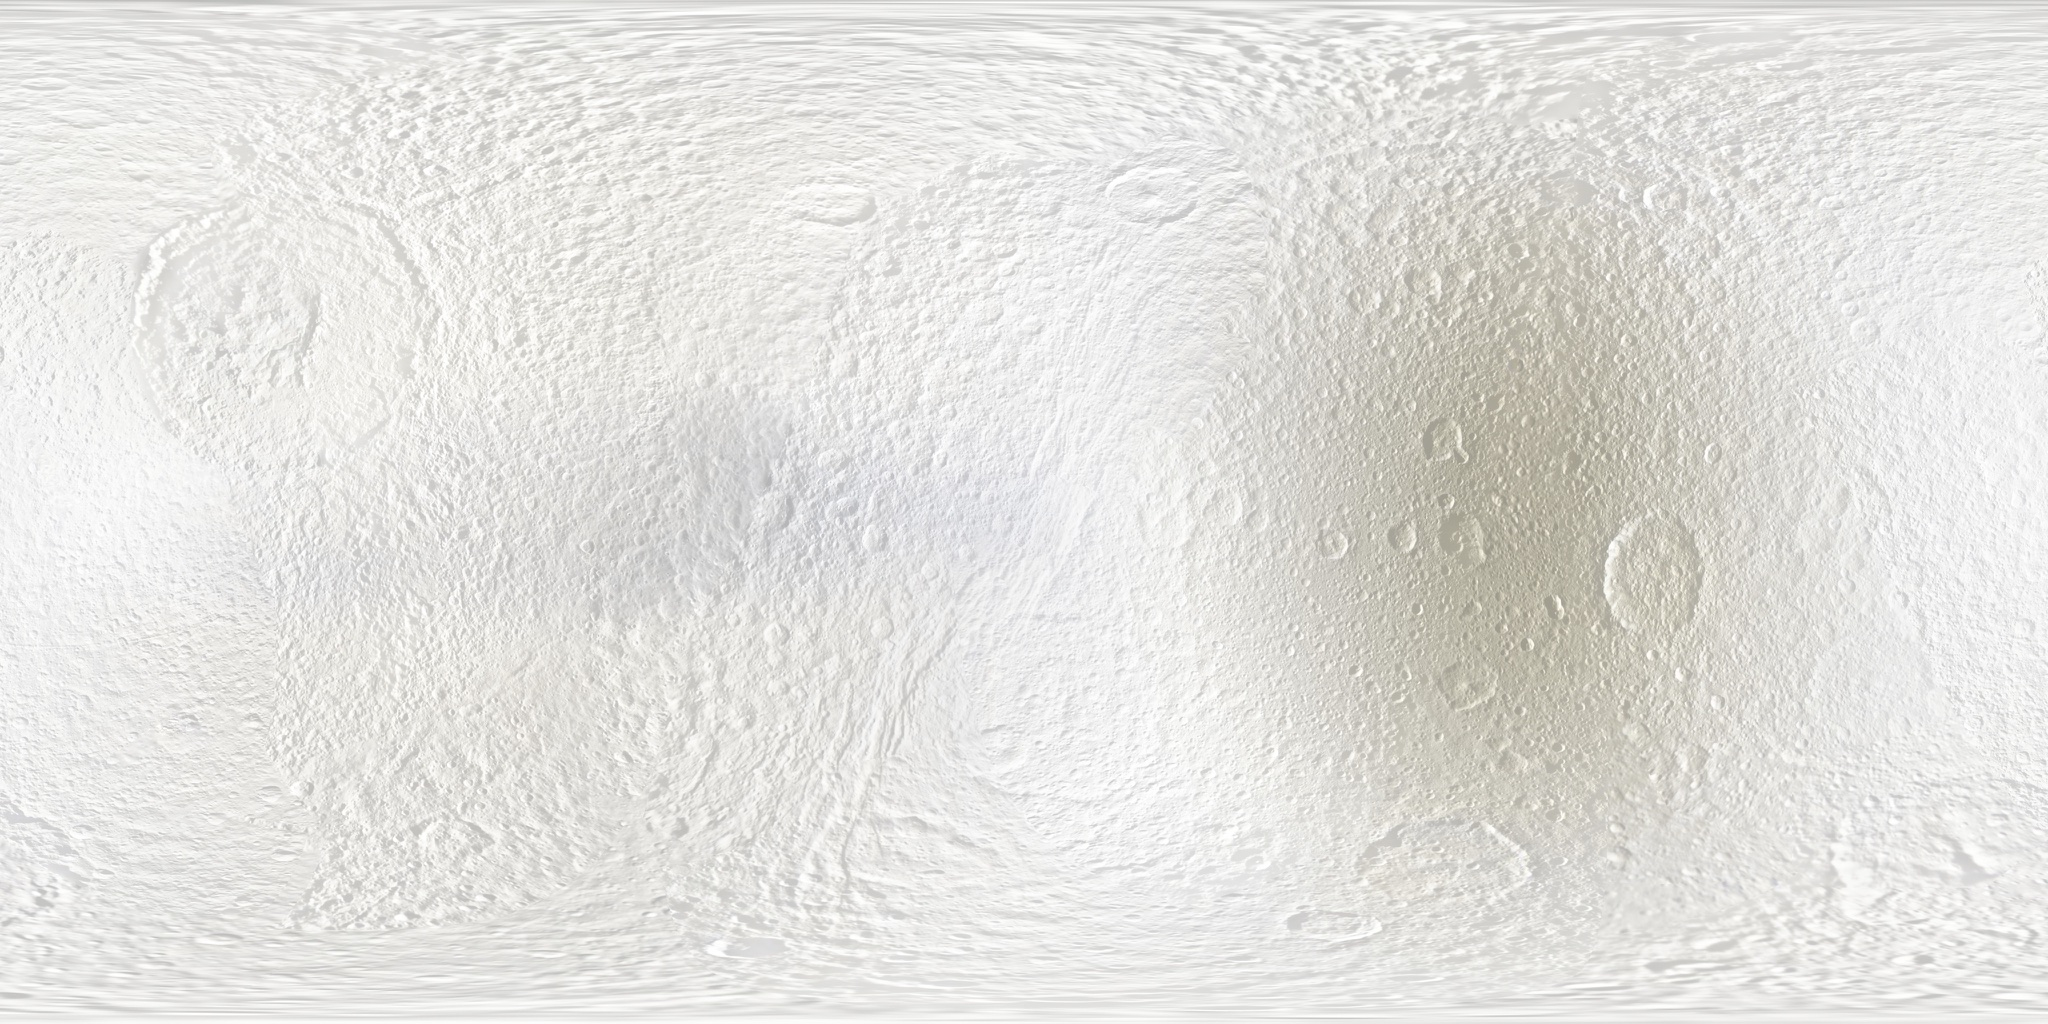
\includegraphics[width=\linewidth,height=4.4cm,keepaspectratio]{../public/textures/hd/tethys_cassini.jpg}\\[2pt]
{\scriptsize\itshape\color{orbitarMuted} Planiglob desfășurat: Harta globală a lunii înghețate Tethys, cu uriașul bazin de impact Odysseus și canionul Ithaca Chasma (NASA/ESA Cassini).}
\end{tabular}
\end{center}


\begin{tcolorbox}[orbitardata, title={\textbf{Repere esențiale: Tethys}}]
\small
\begin{itemize}[leftmargin=1.4em, itemsep=2pt, topsep=2pt]
  \item \textbf{Clasificare și orbită:} Satelit Natural (Lună) (orbitează în jurul: \textbf{Saturn}) \quad$\bullet$\quad \textbf{Distanță:} 9,582 UA ($\approx$ 1.433 milioane de kilometri)
  \item \textbf{Dimensiuni și masă:} rază medie 531,1 de kilometri \quad$\bullet$\quad masă: 1,03e-4 $\times M_\oplus$
  \item \textbf{Gravitație și regim termic:} 0,015 $\times g_\oplus$ (0,15 m/s$^2$) \quad$\bullet$\quad temperatură medie: -187 $^\circ$C (înclinarea axei: Nespecificată)
  \item \textbf{Ciclu orbital și rotație:} perioadă orbitală (an): 1,888 zile pământești \quad$\bullet$\quad rotație (zi): 45,31 ore (1,89 zile pământești)
  \item \textbf{Durata călătoriei de pe Pământ:} cu viteza luminii ($1c$): \emph{1 oră și 11 minute}; cu racheta ($50.000$ de kilometri pe oră): \emph{7 ani}; cu avionul ($900$ de kilometri pe oră): \emph{160 de ani}; cu mașina ($100$ de kilometri pe oră): \emph{1.450 de ani}.
  \item \textbf{Repere de scară și curiozitate:} Pentru că este făcută aproape doar din gheață, Tethys este mai ușoară decât apa, astfel că dacă ai găsi un ocean destul de mare, Tethys ar pluti pe el ca un cub de gheață! Canionul Ithaca Chasma de pe Tethys este lung de 2.000 de kilometri și încinge trei sferturi din întreaga lună ca o centură de gheață!
\end{itemize}
\end{tcolorbox}

\subsubsection*{Prezentare generală și profil astrofizic}
Descoperită de Giovanni Domenico Cassini în 1684, Tethys are cea mai scăzută densitate dintre toți sateliții majori din Sistemul Solar (0,984 g/cm$^3$), indicând că este compusă în proporție de peste 93\% din gheață de apă și mai puțin de 7\% rocă. Tethys este o lună mare și luminoasă a lui Saturn, formată aproape în întregime din gheață curată de apă! Pe ea se află un crater gigant numit Odysseus și o vale imensă de gheață. Pentru că este făcută aproape doar din gheață, Tethys este mai ușoară decât apa, astfel că dacă ai găsi un ocean destul de mare, Tethys ar pluti pe el ca un cub de gheață!

\subsubsection*{Alcătuirea fizică și structura internă}
Privind în profunzimea sa, alcătuirea fizică este organizată pe mai multe straturi și regiuni distincte, fiecare având un rol bine definit în evoluția și dinamica acestui obiect cosmic. În primul rând se remarcă \textbf{Interior omogen de gheață de apă}, densitatea de 0,984 g/cm$^3$ arată că fracțiunea stâncoasă este minimă. În strânsă legătură cu această componentă se află \textbf{Bazinul de impact Odysseus (445 de kilometri diametru)}, un crater colosal lat cât două cincimi din diametrul satelitului, ale cărui margini s-au aplatizat în timp prin relaxarea vâscoasă a gheții. În completarea acestui ansamblu întâlnim \textbf{Sistemul tectonic Ithaca Chasma}, o vale ramificată lată de 100 de kilometri, adâncă de 3--5 kilometri și lungă de 2.000 de kilometri, formată când oceanul intern străvechi al lui Tethys a înghețat și s-a dilatat.

\subsubsection*{Observații astronomice și istoricul explorării}
Fotografiată de Pioneer 11 și Voyager 1/2 și cartografiată la înaltă rezoluție de sonda Cassini în timpul survolului apropiat din septembrie 2005. Canionul Ithaca Chasma de pe Tethys este lung de 2.000 de kilometri și încinge trei sferturi din întreaga lună ca o centură de gheață!

\vspace{6pt}
\begin{tcolorbox}[orbitarquiz, title={\textbf{Întrebare de verificare \#17: Tethys}}]
\textbf{Din ce material este alcătuită în proporție de peste 93\% luna Tethys a lui Saturn?}
\begin{itemize}[leftmargin=2.2em, itemsep=2pt, topsep=4pt]
  \item[$\square$ \textbf{A.}] Din fier topit
  \item[$\square$ \textbf{B.}] Din gheață de apă aproape pură (având o densitate mai mică decât a apei lichide)
  \item[$\square$ \textbf{C.}] Din gaz metan
  \item[$\square$ \textbf{D.}] Din bazalt vulcanic negru
\end{itemize}
\vspace{2pt}
{\footnotesize\color{orbitarMuted}\textbf{Răspuns corect:} \textbf{B} (Din gheață de apă aproape pură (având o densitate mai mică decât a apei lichide)). \emph{Cu o densitate medie de 0,984 g/cm$^3$, Tethys este alcătuită aproape exclusiv din gheață de apă, reflectând puternic lumina Soarelui.}}
\end{tcolorbox}
\clearpage


\subsection{Dione}
\label{sec:body-dione}
\vspace{-4pt}
{\large\itshape\color{orbitarAccent} Luna înghețată a lui Saturn, brăzdată de faleze tectonice strălucitoare}\\[4pt]


\begin{center}
\begin{tabular}{@{}m{0.44\textwidth}@{\hspace{0.03\textwidth}}m{0.51\textwidth}@{}}
\centering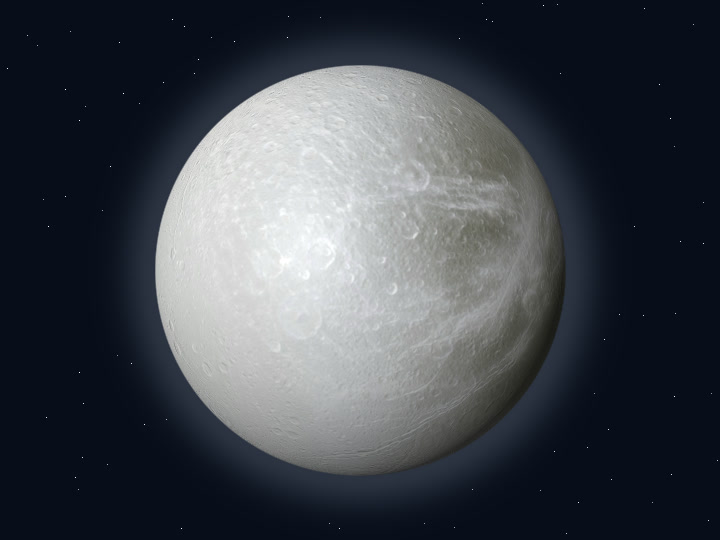
\includegraphics[width=\linewidth,height=4.4cm,keepaspectratio]{imagini/globuri/dione.jpg}\\[2pt]
{\scriptsize\itshape\color{orbitarMuted} Vedere 3D a corpului ceresc (\textbf{Dione})}
&
\centering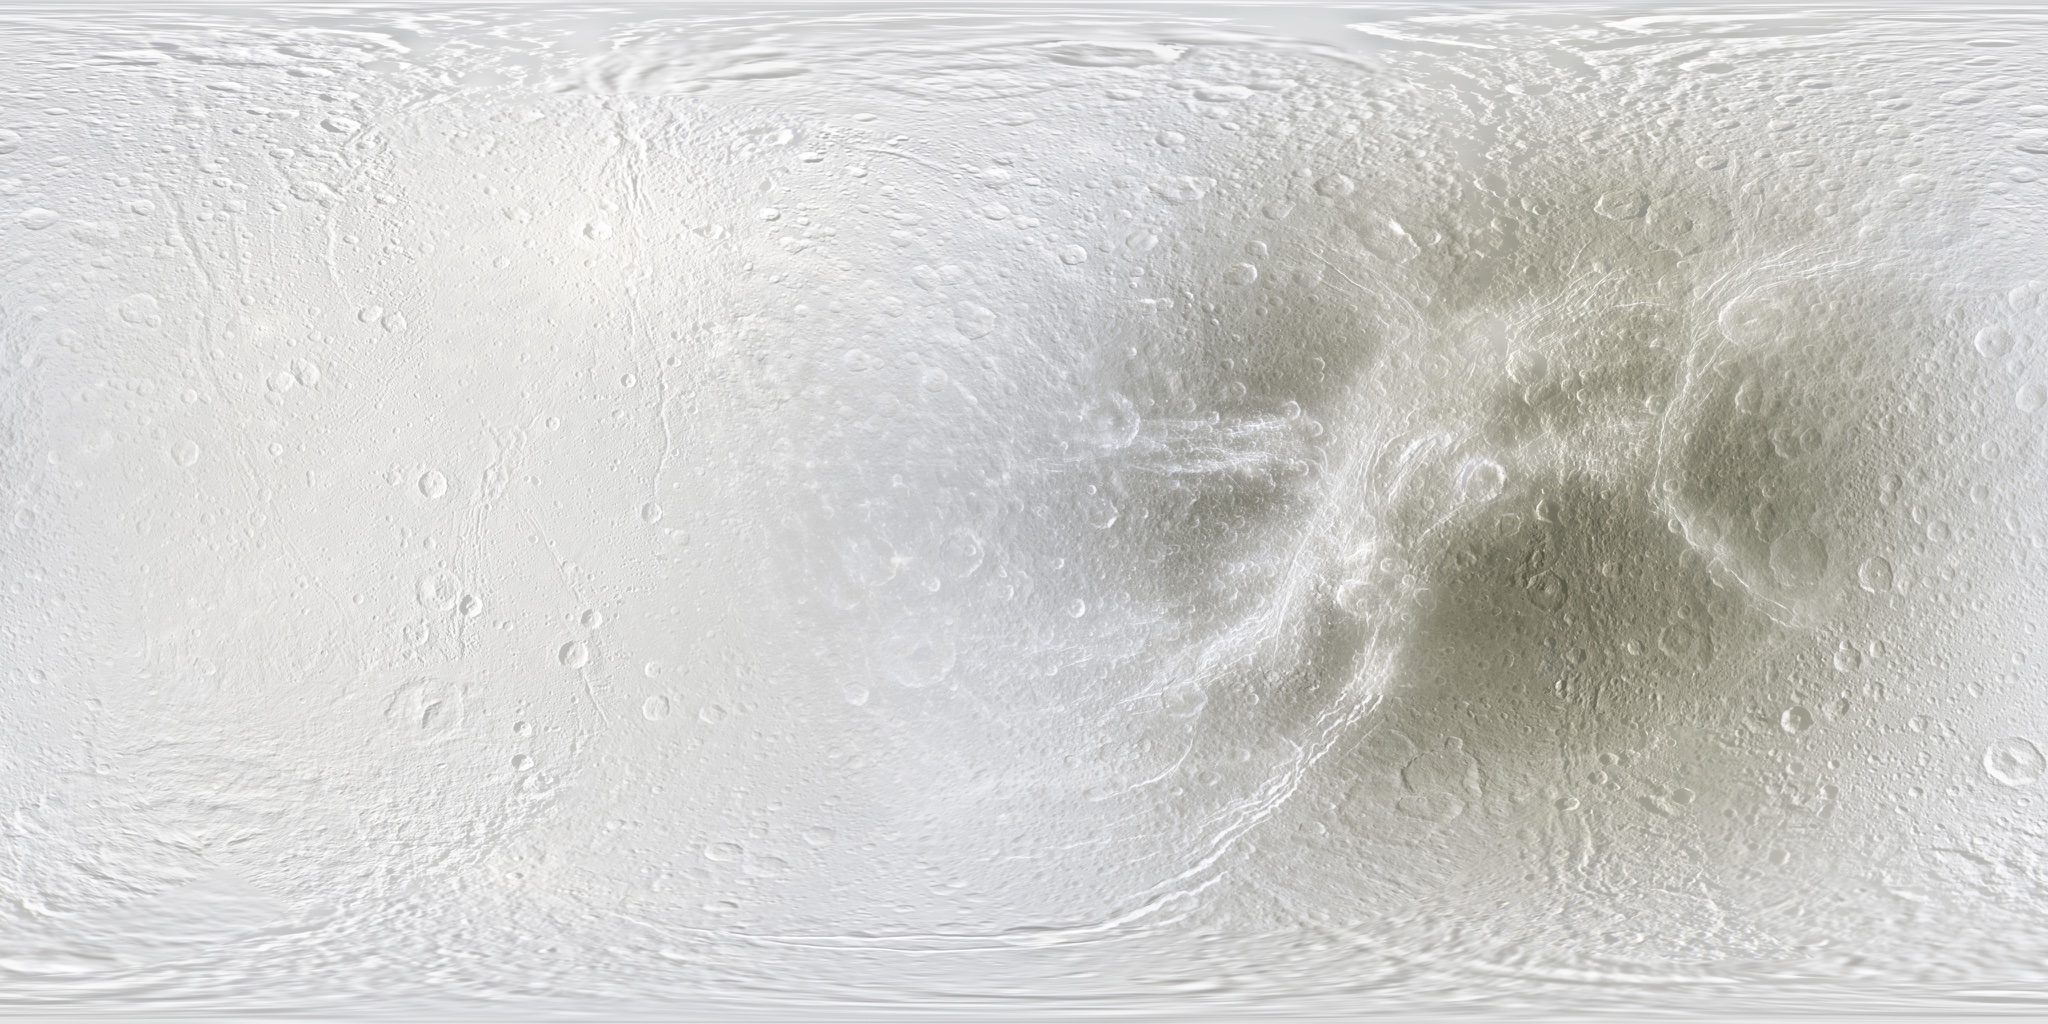
\includegraphics[width=\linewidth,height=4.4cm,keepaspectratio]{../public/textures/hd/dione_cassini.jpg}\\[2pt]
{\scriptsize\itshape\color{orbitarMuted} Planiglob desfășurat: Harta globală a lunii Dione și a falezelor luminoase de gheață Padua Chasmata (NASA/ESA Cassini).}
\end{tabular}
\end{center}


\begin{tcolorbox}[orbitardata, title={\textbf{Repere esențiale: Dione}}]
\small
\begin{itemize}[leftmargin=1.4em, itemsep=2pt, topsep=2pt]
  \item \textbf{Clasificare și orbită:} Satelit Natural (Lună) (orbitează în jurul: \textbf{Saturn}) \quad$\bullet$\quad \textbf{Distanță:} 9,582 UA ($\approx$ 1.433 milioane de kilometri)
  \item \textbf{Dimensiuni și masă:} rază medie 561,4 de kilometri \quad$\bullet$\quad masă: 1,83e-4 $\times M_\oplus$
  \item \textbf{Gravitație și regim termic:} 0,024 $\times g_\oplus$ (0,24 m/s$^2$) \quad$\bullet$\quad temperatură medie: -186 $^\circ$C (înclinarea axei: Nespecificată)
  \item \textbf{Ciclu orbital și rotație:} perioadă orbitală (an): 2,737 zile pământești \quad$\bullet$\quad rotație (zi): 65,69 ore (2,74 zile pământești)
  \item \textbf{Durata călătoriei de pe Pământ:} cu viteza luminii ($1c$): \emph{1 oră și 11 minute}; cu racheta ($50.000$ de kilometri pe oră): \emph{7 ani}; cu avionul ($900$ de kilometri pe oră): \emph{160 de ani}; cu mașina ($100$ de kilometri pe oră): \emph{1.450 de ani}.
  \item \textbf{Repere de scară și curiozitate:} Rețeaua de stânci luminoase de pe Dione arată din spațiu ca niște fire subțiri de beteală argintie așezate pe un glob înghețat! Două luni mici, Helene și Polydeuces, călătoresc pe exact aceeași orbită cu Dione, una în fața ei și cealaltă în urma ei!
\end{itemize}
\end{tcolorbox}

\subsubsection*{Prezentare generală și profil astrofizic}
Descoperită tot de Cassini în 1684, Dione are un diametru de 1.123 de kilometri și o densitate de 1,48 g/cm$^3$ (a treia cea mai mare dintre sateliții lui Saturn, după Titan și Enceladus), având un nucleu substanțial de silicați și posibil un ocean subteran sub o crustă groasă de gheață. Dione este a patra lună ca mărime a lui Saturn! Pe o parte a ei se văd dungi albe și sclipitoare care sunt, de fapt, stânci uriașe de gheață curată! Rețeaua de stânci luminoase de pe Dione arată din spațiu ca niște fire subțiri de beteală argintie așezate pe un glob înghețat!

\subsubsection*{Alcătuirea fizică și structura internă}
Privind în profunzimea sa, alcătuirea fizică este organizată pe mai multe straturi și regiuni distincte, fiecare având un rol bine definit în evoluția și dinamica acestui obiect cosmic. În primul rând se remarcă \textbf{Nucleu stâncos de silicați (aproximativ 46\% din masă)}, îi conferă o densitate semnificativ mai ridicată decât cea a vecinei Tethys. În strânsă legătură cu această componentă se află \textbf{Posibil ocean subglaciar profund}, indicat de datele gravimetrice și de topografie ale misiunii Cassini, situat la aproximativ 100 de kilometri sub suprafață. În completarea acestui ansamblu întâlnim \textbf{Falezele tectonice din Padua Chasmata}, fracturi de gheață luminoase înalte de sute de metri pe emisfera posterioară, cunoscute inițial drept \guillemotleft{}terenul vălurit\guillemotright{} (wispy terrain).

\subsubsection*{Observații astronomice și istoricul explorării}
Fotografiată de sondele Voyager și studiată în cinci survoluri apropiate de sonda Cassini între 2005 și 2015, care a detectat o exosferă extrem de rarefiată de ioni de oxigen. Două luni mici, Helene și Polydeuces, călătoresc pe exact aceeași orbită cu Dione, una în fața ei și cealaltă în urma ei!

\vspace{6pt}
\begin{tcolorbox}[orbitarquiz, title={\textbf{Întrebare de verificare \#18: Dione}}]
\textbf{Ce s-au dovedit a fi în realitate dungile albe luminoase (\guillemotleft{}wispy terrain\guillemotright{}) de pe satelitul Dione, fotografiate de aproape de sonda Cassini?}
\begin{itemize}[leftmargin=2.2em, itemsep=2pt, topsep=4pt]
  \item[$\square$ \textbf{A.}] Nori de ploaie
  \item[$\square$ \textbf{B.}] Faleze și canioane tectonice abrupte din gheață strălucitoare (precum Padua Chasmata)
  \item[$\square$ \textbf{C.}] Râuri de lavă
  \item[$\square$ \textbf{D.}] Dune de nisip galben
\end{itemize}
\vspace{2pt}
{\footnotesize\color{orbitarMuted}\textbf{Răspuns corect:} \textbf{B} (Faleze și canioane tectonice abrupte din gheață strălucitoare (precum Padua Chasmata)). \emph{Imaginile de înaltă rezoluție de la Cassini au arătat că dungile luminoase sunt pereți abrupți de falii tectonice unde gheața curată este expusă la suprafață.}}
\end{tcolorbox}
\clearpage


\subsection{Rhea}
\label{sec:body-rhea}
\vspace{-4pt}
{\large\itshape\color{orbitarAccent} A doua lună ca mărime a lui Saturn, un corp străvechi de gheață și stâncă}\\[4pt]


\begin{center}
\begin{tabular}{@{}m{0.44\textwidth}@{\hspace{0.03\textwidth}}m{0.51\textwidth}@{}}
\centering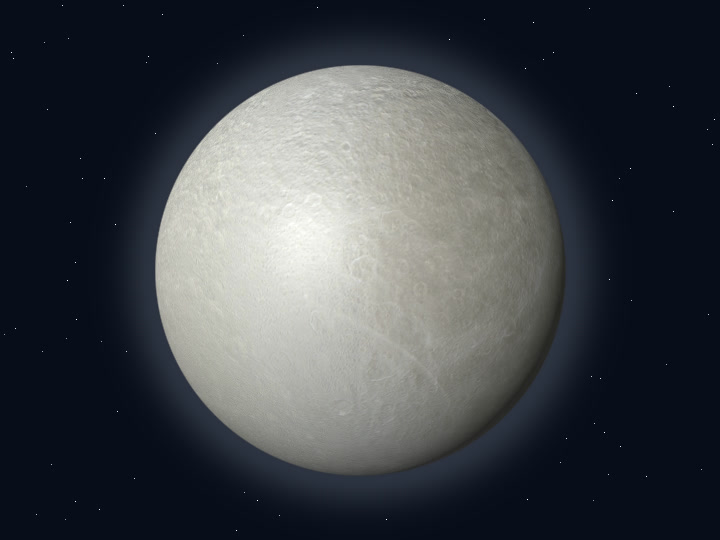
\includegraphics[width=\linewidth,height=4.4cm,keepaspectratio]{imagini/globuri/rhea.jpg}\\[2pt]
{\scriptsize\itshape\color{orbitarMuted} Vedere 3D a corpului ceresc (\textbf{Rhea})}
&
\centering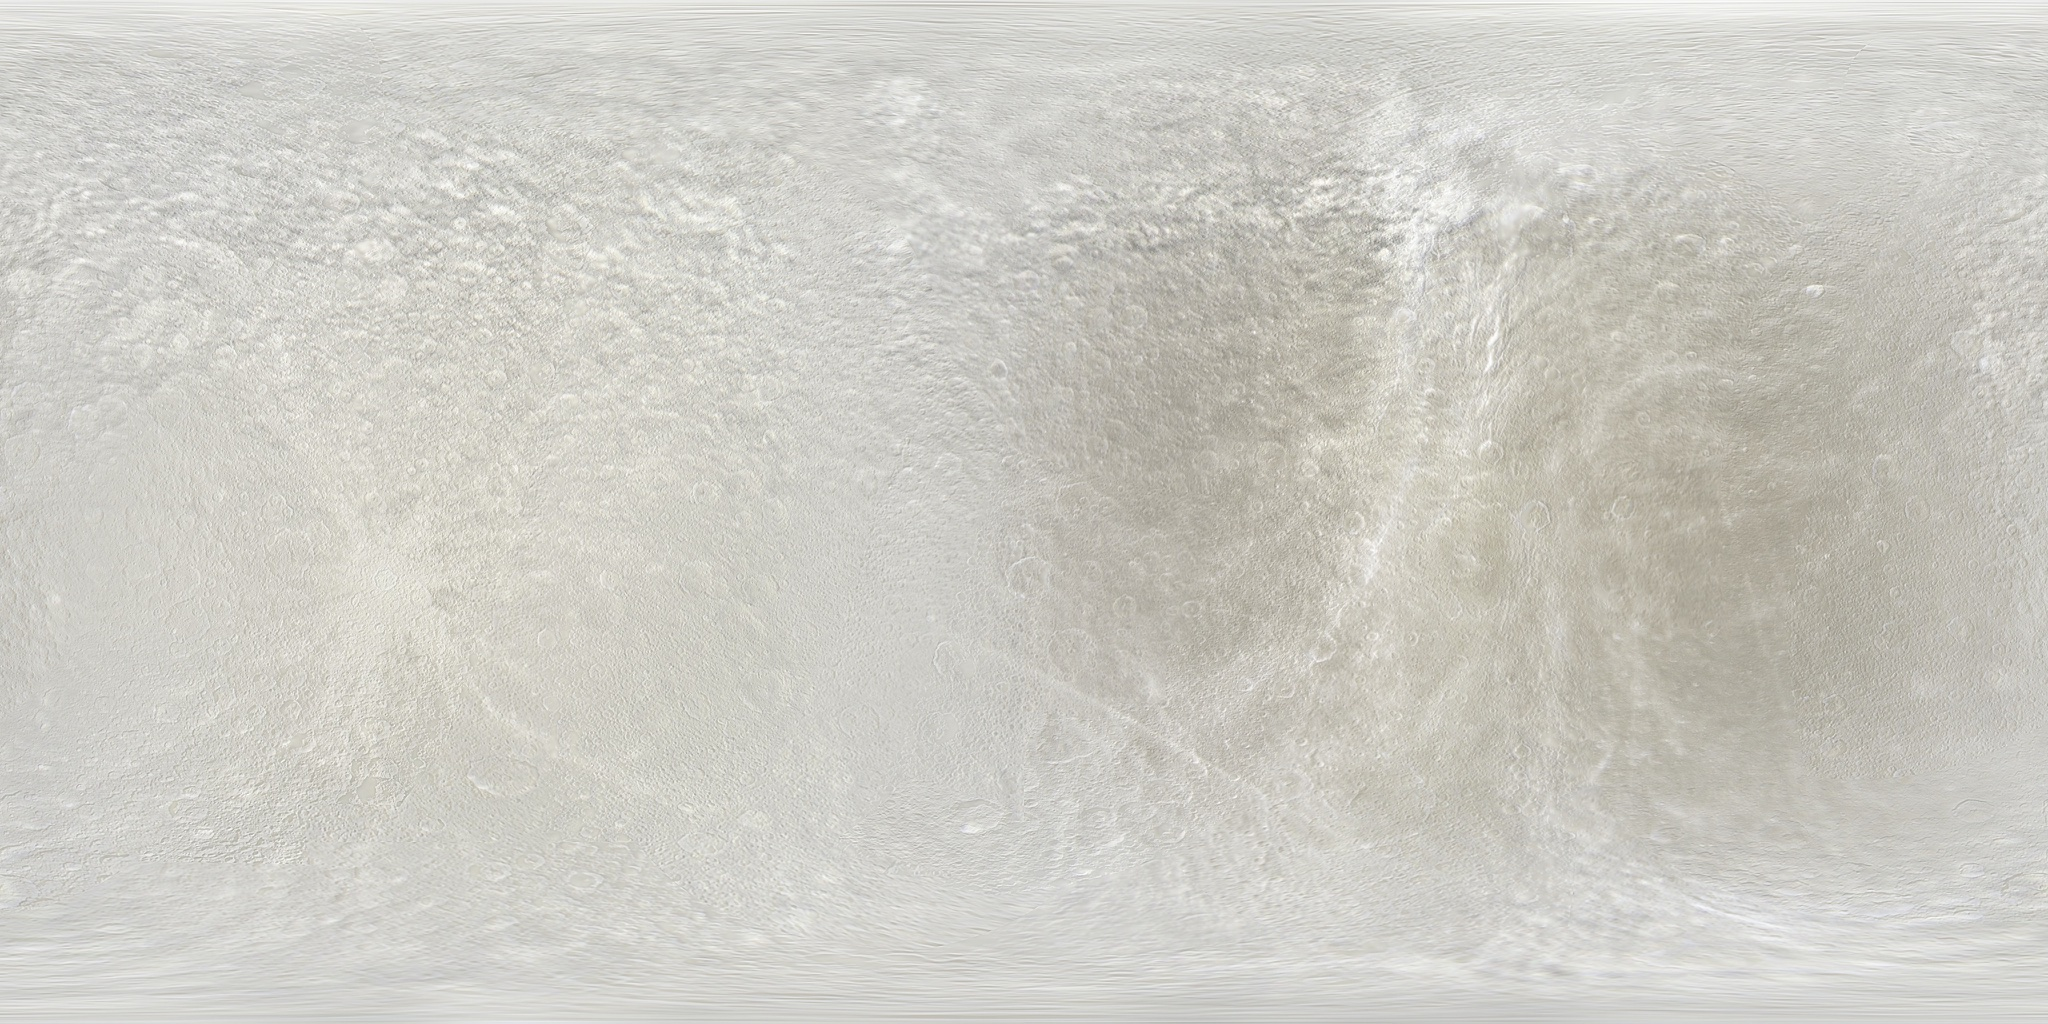
\includegraphics[width=\linewidth,height=4.4cm,keepaspectratio]{../public/textures/hd/rhea_cassini.jpg}\\[2pt]
{\scriptsize\itshape\color{orbitarMuted} Planiglob desfășurat: Suprafața intens craterizată a lunii Rhea, al doilea satelit ca mărime al lui Saturn (NASA/ESA Cassini).}
\end{tabular}
\end{center}


\begin{tcolorbox}[orbitardata, title={\textbf{Repere esențiale: Rhea}}]
\small
\begin{itemize}[leftmargin=1.4em, itemsep=2pt, topsep=2pt]
  \item \textbf{Clasificare și orbită:} Satelit Natural (Lună) (orbitează în jurul: \textbf{Saturn}) \quad$\bullet$\quad \textbf{Distanță:} 9,582 UA ($\approx$ 1.433 milioane de kilometri)
  \item \textbf{Dimensiuni și masă:} rază medie 763,8 de kilometri \quad$\bullet$\quad masă: 3,86e-4 $\times M_\oplus$
  \item \textbf{Gravitație și regim termic:} 0,027 $\times g_\oplus$ (0,26 m/s$^2$) \quad$\bullet$\quad temperatură medie: -197 $^\circ$C (înclinarea axei: Nespecificată)
  \item \textbf{Ciclu orbital și rotație:} perioadă orbitală (an): 4,518 zile pământești \quad$\bullet$\quad rotație (zi): 108,43 ore (4,52 zile pământești)
  \item \textbf{Durata călătoriei de pe Pământ:} cu viteza luminii ($1c$): \emph{1 oră și 11 minute}; cu racheta ($50.000$ de kilometri pe oră): \emph{7 ani}; cu avionul ($900$ de kilometri pe oră): \emph{160 de ani}; cu mașina ($100$ de kilometri pe oră): \emph{1.450 de ani}.
  \item \textbf{Repere de scară și curiozitate:} Rhea are un diametru de peste 1.500 de kilometri, fiind de aproape trei ori mai lată decât România! Sonda Cassini a descoperit în jurul lui Rhea o atmosferă extrem de subțire care conține oxigen și dioxid de carbon!
\end{itemize}
\end{tcolorbox}

\subsubsection*{Prezentare generală și profil astrofizic}
Descoperită în 1672 de Giovanni Domenico Cassini, Rhea este al nouălea satelit ca mărime din Sistemul Solar (diametru de 1.527,6 kilometri). Are o suprafață intens craterizată, împărțită între o emisferă anterioară luminoasă și o emisferă posterioară întunecată, brăzdată de canioane de gheață. Rhea este sora mai mare a lunilor de gheață ale lui Saturn și a doua lună ca mărime a planetei, imediat după uriașul Titan! Rhea are un diametru de peste 1.500 de kilometri, fiind de aproape trei ori mai lată decât România!

\subsubsection*{Alcătuirea fizică și structura internă}
Privind în profunzimea sa, alcătuirea fizică este organizată pe mai multe straturi și regiuni distincte, fiecare având un rol bine definit în evoluția și dinamica acestui obiect cosmic. În primul rând se remarcă \textbf{Interior slab diferențiat (75\% gheață, 25\% rocă)}, densitatea medie de 1,236 g/cm$^3$ indică un amestec de gheață de apă și roci silicatice. În strânsă legătură cu această componentă se află \textbf{Bazinele de impact Tirawa și Mamaldi}, două bazine străvechi uriașe (de 360 de kilometri și 480 de kilometri diametru) și craterul tânăr Inktomi cu raze strălucitoare de gheață pură. În completarea acestui ansamblu întâlnim \textbf{Exosferă fină de oxigen (O$_2$) și dioxid de carbon (CO$_2$)}, eliberată prin radioliza gheții de la suprafață sub acțiunea ionilor din magnetosfera lui Saturn.

\subsubsection*{Observații astronomice și istoricul explorării}
Fotografiată de sondele Voyager 1 și 2 și explorată îndeaproape de sonda Cassini (inclusiv un survol la doar 50 de kilometri altitudine în martie 2010). Sonda Cassini a descoperit în jurul lui Rhea o atmosferă extrem de subțire care conține oxigen și dioxid de carbon!

\vspace{6pt}
\begin{tcolorbox}[orbitarquiz, title={\textbf{Întrebare de verificare \#19: Rhea}}]
\textbf{Ce loc ocupă Rhea ca mărime între sateliții planetei Saturn?}
\begin{itemize}[leftmargin=2.2em, itemsep=2pt, topsep=4pt]
  \item[$\square$ \textbf{A.}] Este cel mai mic satelit
  \item[$\square$ \textbf{B.}] Este al doilea satelit ca mărime al lui Saturn, după Titan
  \item[$\square$ \textbf{C.}] Este mai mare decât Saturn
  \item[$\square$ \textbf{D.}] Este pe locul zece
\end{itemize}
\vspace{2pt}
{\footnotesize\color{orbitarMuted}\textbf{Răspuns corect:} \textbf{B} (Este al doilea satelit ca mărime al lui Saturn, după Titan). \emph{Cu o rază de 763,8 kilometri (diametru de 1.528 de kilometri), Rhea este a doua lună ca mărime a lui Saturn, fiind depășită doar de Titan.}}
\end{tcolorbox}
\clearpage


\subsection{Titan}
\label{sec:body-titan}
\vspace{-4pt}
{\large\itshape\color{orbitarAccent} Satelitul lui Saturn cu atmosferă densă și lacuri de metan}\\[4pt]


\begin{center}
\begin{tabular}{@{}m{0.44\textwidth}@{\hspace{0.03\textwidth}}m{0.51\textwidth}@{}}
\centering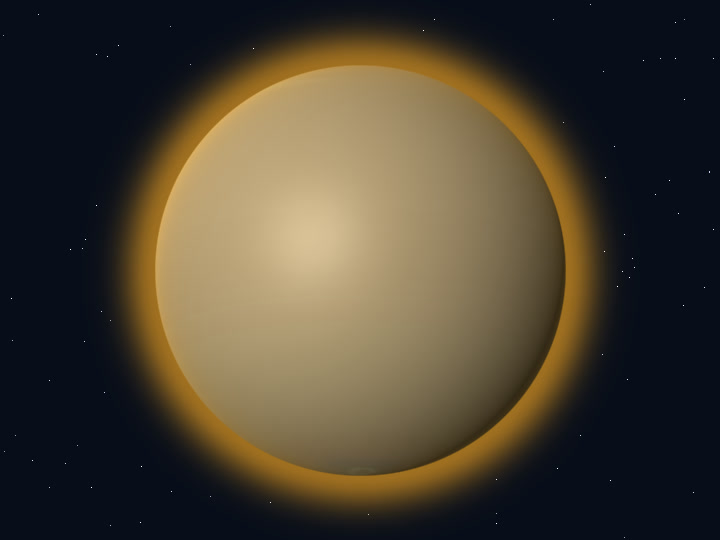
\includegraphics[width=\linewidth,height=4.4cm,keepaspectratio]{imagini/globuri/titan.jpg}\\[2pt]
{\scriptsize\itshape\color{orbitarMuted} Vedere 3D a corpului ceresc (\textbf{Titan})}
&
\centering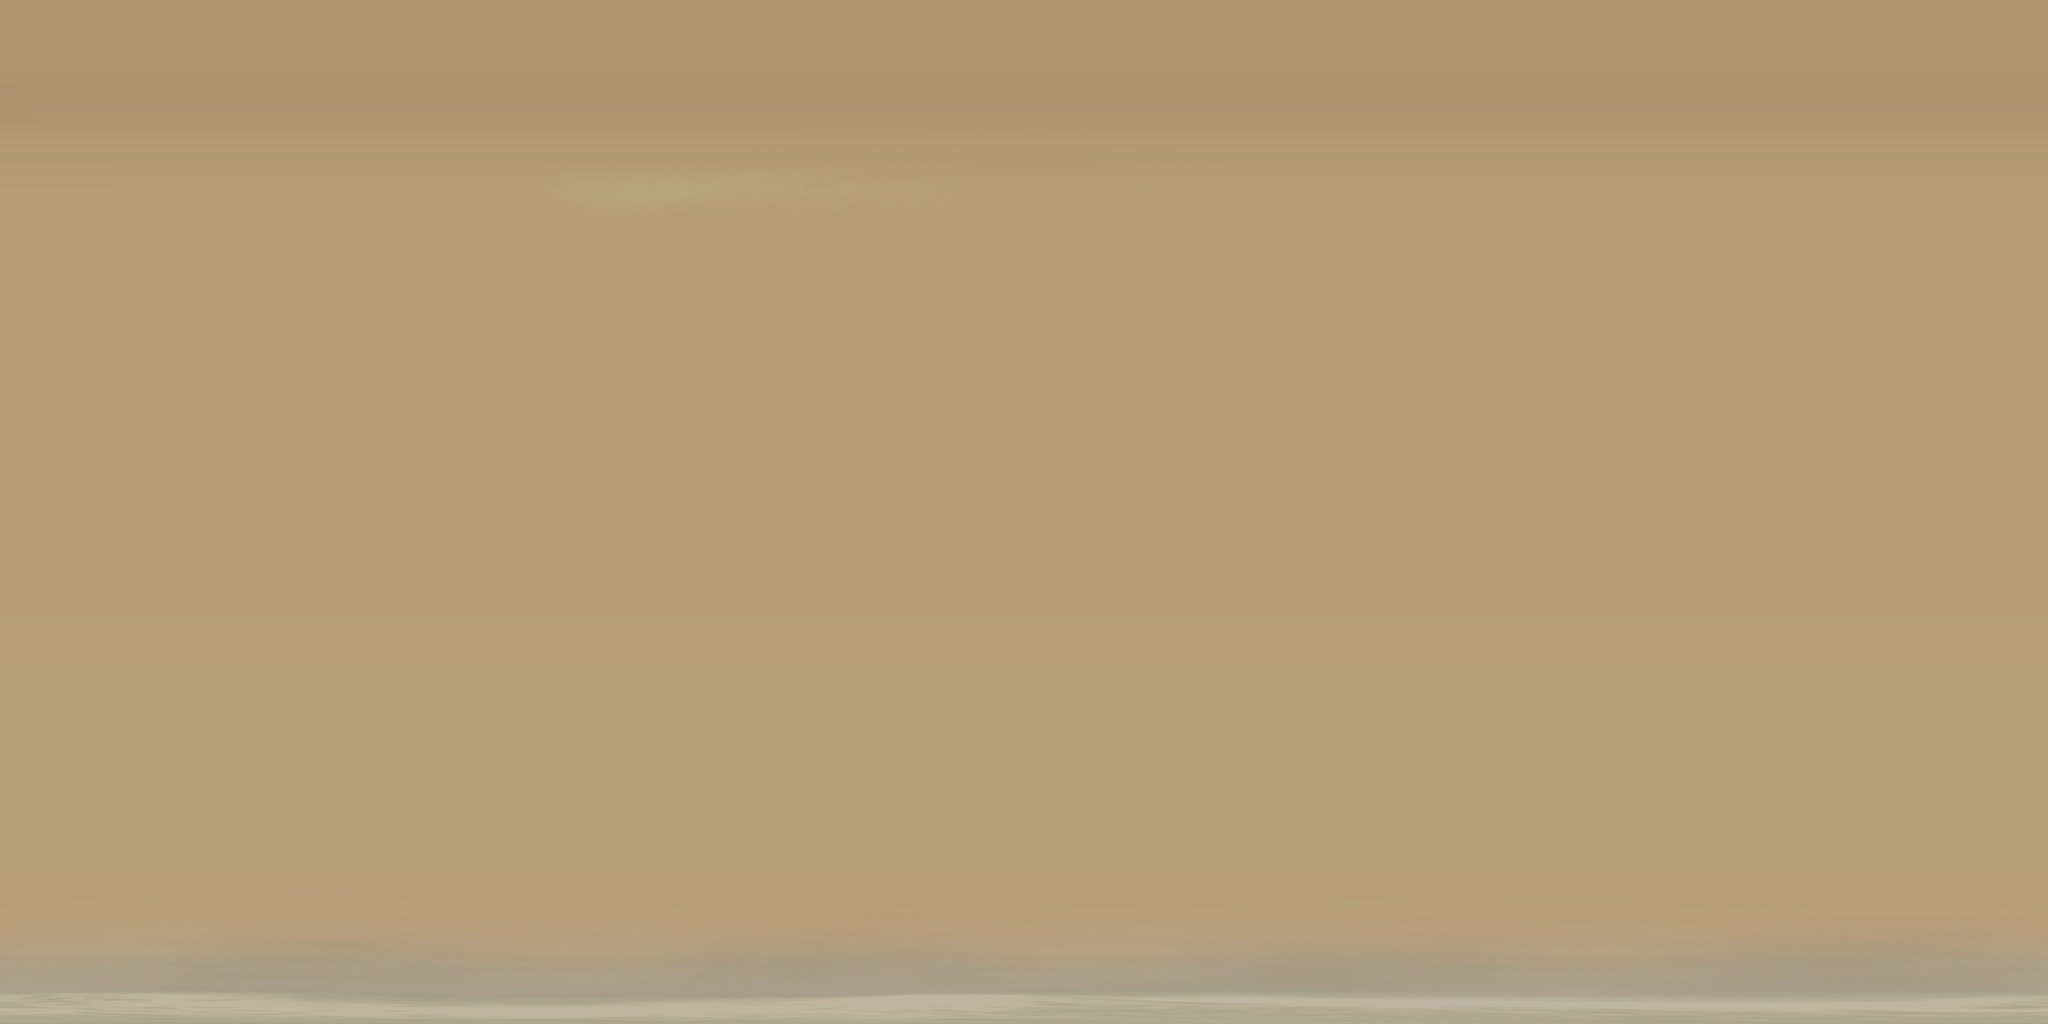
\includegraphics[width=\linewidth,height=4.4cm,keepaspectratio]{../public/textures/hd/titan_cassini.jpg}\\[2pt]
{\scriptsize\itshape\color{orbitarMuted} Planiglob desfășurat: Harta globală a lunii Titan obținută prin străpungerea ceții portocalii de azot și metan de către sonda Cassini.}
\end{tabular}
\end{center}


\begin{tcolorbox}[orbitardata, title={\textbf{Repere esențiale: Titan}}]
\small
\begin{itemize}[leftmargin=1.4em, itemsep=2pt, topsep=2pt]
  \item \textbf{Clasificare și orbită:} Satelit Natural (Lună) (orbitează în jurul: \textbf{Saturn}) \quad$\bullet$\quad \textbf{Distanță:} 9,582 UA ($\approx$ 1.433 milioane de kilometri)
  \item \textbf{Dimensiuni și masă:} rază medie 2.574,7 de kilometri \quad$\bullet$\quad masă: 0,022 $\times M_\oplus$
  \item \textbf{Gravitație și regim termic:} 0,138 $\times g_\oplus$ (1,35 m/s$^2$) \quad$\bullet$\quad temperatură medie: -179 $^\circ$C (înclinarea axei: Nespecificată)
  \item \textbf{Ciclu orbital și rotație:} perioadă orbitală (an): 15,945 zile pământești \quad$\bullet$\quad rotație (zi): 382,68 ore (15,95 zile pământești)
  \item \textbf{Durata călătoriei de pe Pământ:} cu viteza luminii ($1c$): \emph{1 oră și 11 minute}; cu racheta ($50.000$ de kilometri pe oră): \emph{7 ani}; cu avionul ($900$ de kilometri pe oră): \emph{160 de ani}; cu mașina ($100$ de kilometri pe oră): \emph{1.450 de ani}.
  \item \textbf{Repere de scară și curiozitate:} Pe Titan atmosfera e atât de deasă și gravitația atât de mică încât, dacă ți-ai pune aripi pe brațe, ai putea zbura dând din mâini ca o pasăre! Râurile și lacurile de pe Titan nu sunt din apă, ci din metan și etan lichid, la aproape -180 $^\circ$C!
\end{itemize}
\end{tcolorbox}

\subsubsection*{Prezentare generală și profil astrofizic}
Al doilea satelit ca mărime din Sistemul Solar (mai mare decât Mercur), Titan este singurul satelit cu o atmosferă densă (97\% azot, presiune de 1,45 ori mai mare decât pe Pământ) și singurul corp în afară de Pământ cu lichid stabil la suprafață. Titan este cea mai mare lună a lui Saturn și singura lună învelită într-o atmosferă groasă și portocalie, cu nori, ploi, râuri și mări! Pe Titan atmosfera e atât de deasă și gravitația atât de mică încât, dacă ți-ai pune aripi pe brațe, ai putea zbura dând din mâini ca o pasăre!

\subsubsection*{Alcătuirea fizică și structura internă}
Privind în profunzimea sa, alcătuirea fizică este organizată pe mai multe straturi și regiuni distincte, fiecare având un rol bine definit în evoluția și dinamica acestui obiect cosmic. În primul rând se remarcă \textbf{Nucleu de silicați hidratati}, cu o rază de aproximativ 2.000 de kilometri în centrul satelitului. În strânsă legătură cu această componentă se află \textbf{Ocean subteran de apă și amoniac}, situat sub o crustă de gheață de apă dură ca roca. În completarea acestui ansamblu întâlnim \textbf{Suprafață cu ciclu al metanului și atmosferă de azot}, mări de hidrocarburi (Kraken Mare, Ligeia Mare), dune organice și ceață fotochimică (toline).

\subsubsection*{Observații astronomice și istoricul explorării}
Sonda europeană Huygens a asolizat pe Titan în ianuarie 2005 (cea mai îndepărtată asolizare din istorie); NASA pregătește drona nucleară Dragonfly. Râurile și lacurile de pe Titan nu sunt din apă, ci din metan și etan lichid, la aproape -180 $^\circ$C!

\vspace{6pt}
\begin{tcolorbox}[orbitarquiz, title={\textbf{Întrebare de verificare \#20: Titan}}]
\textbf{Din ce sunt formate lacurile și mările de la suprafața lui Titan?}
\begin{itemize}[leftmargin=2.2em, itemsep=2pt, topsep=4pt]
  \item[$\square$ \textbf{A.}] Din apă caldă
  \item[$\square$ \textbf{B.}] Din metan și etan lichid
  \item[$\square$ \textbf{C.}] Din lavă topită
  \item[$\square$ \textbf{D.}] Din mercur lichid
\end{itemize}
\vspace{2pt}
{\footnotesize\color{orbitarMuted}\textbf{Răspuns corect:} \textbf{B} (Din metan și etan lichid). \emph{La temperatura de -179 $^\circ$C de pe Titan, apa este tare ca piatra, iar metanul și etanul formează nori, ploi, râuri și mări.}}
\end{tcolorbox}
\clearpage


\subsection{Hyperion}
\label{sec:body-hyperion}
\vspace{-4pt}
{\large\itshape\color{orbitarAccent} Luna-burete a lui Saturn, cu cratere în formă de fagure și rotație haotică}\\[4pt]


\begin{center}
\begin{tabular}{@{}m{0.44\textwidth}@{\hspace{0.03\textwidth}}m{0.51\textwidth}@{}}
\centering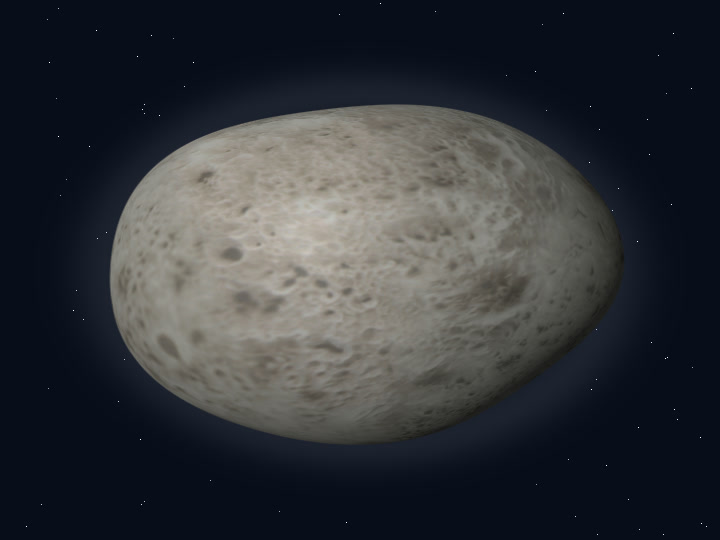
\includegraphics[width=\linewidth,height=4.4cm,keepaspectratio]{imagini/globuri/hyperion.jpg}\\[2pt]
{\scriptsize\itshape\color{orbitarMuted} Vedere 3D a corpului ceresc (\textbf{Hyperion})}
&
\centering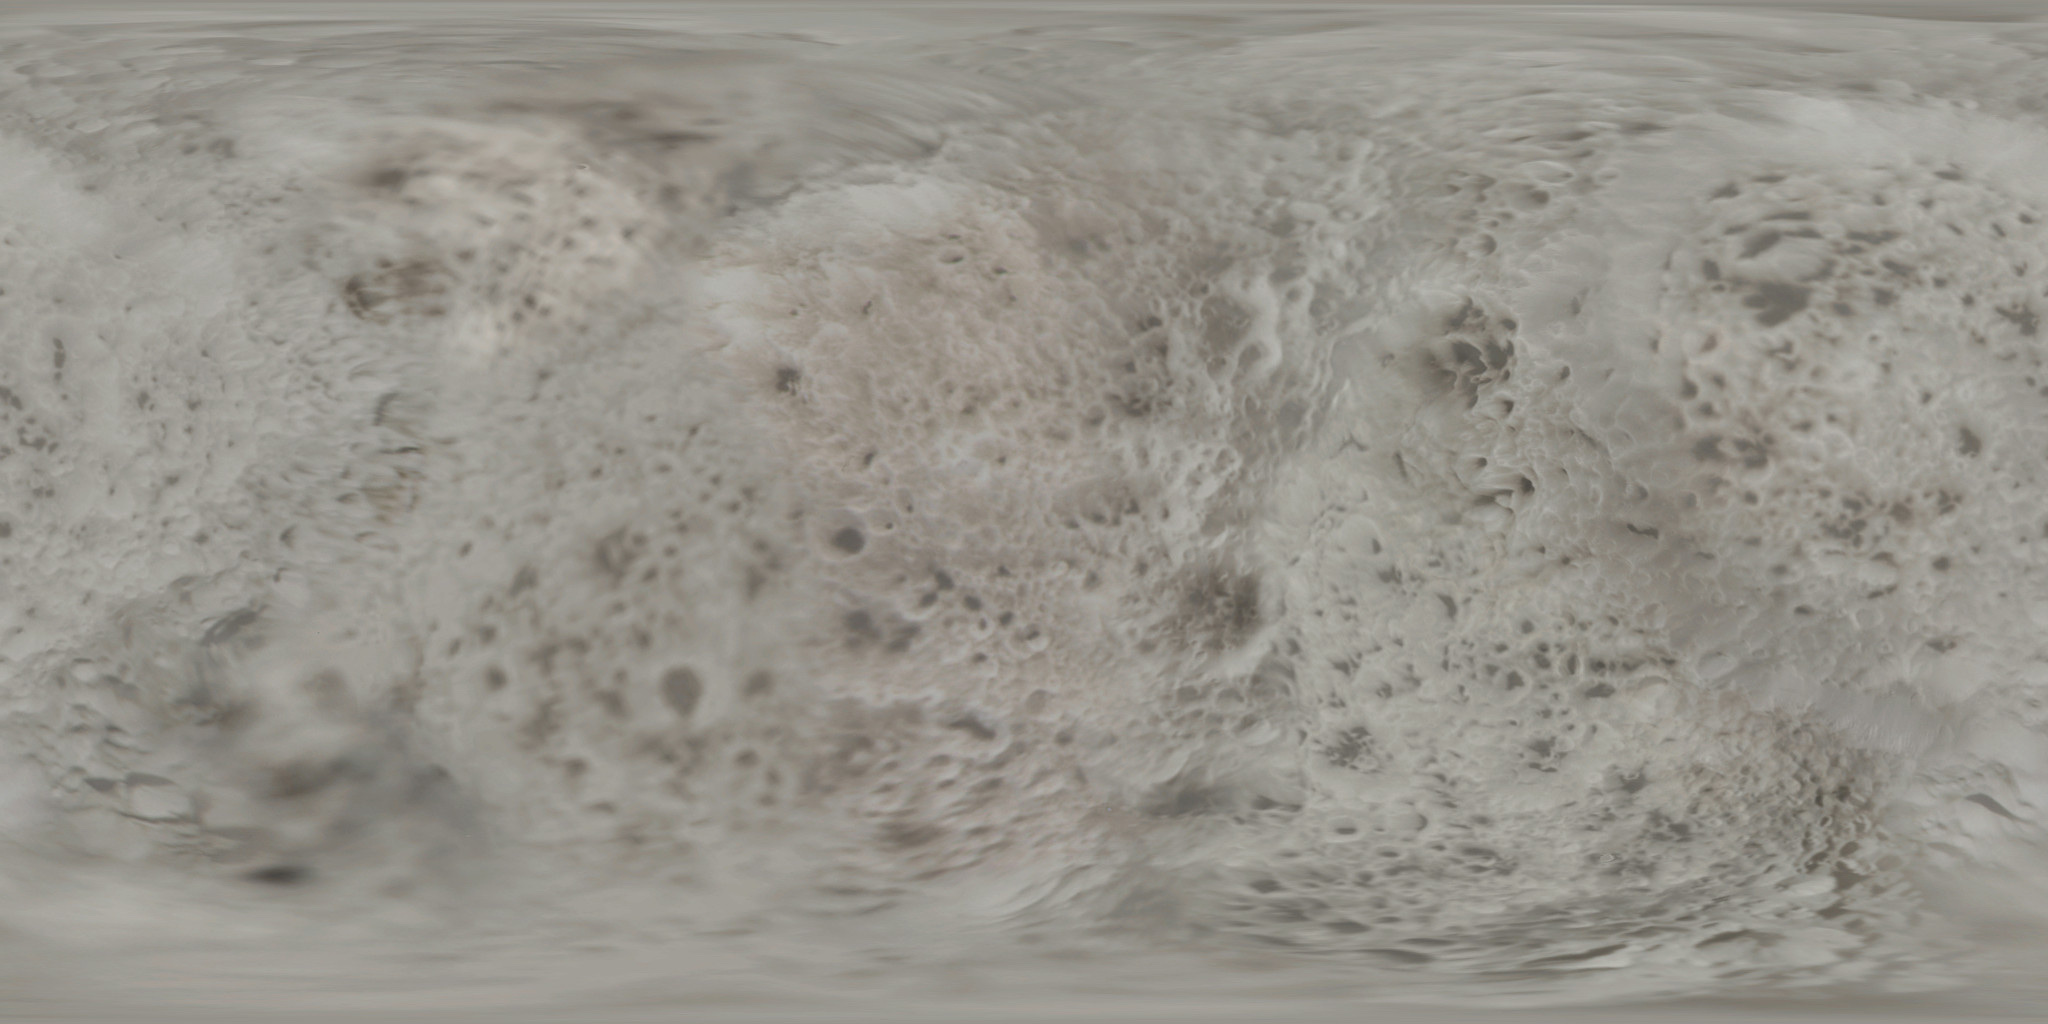
\includegraphics[width=\linewidth,height=4.4cm,keepaspectratio]{../public/textures/hd/hyperion_cassini.jpg}\\[2pt]
{\scriptsize\itshape\color{orbitarMuted} Planiglob desfășurat: Aspectul poros, de \quotedblbase{}burete cosmic\textquotedblright{} ciuruit de cratere adânci, al satelitului cu rotație haotică Hyperion (NASA/ESA Cassini).}
\end{tabular}
\end{center}


\begin{tcolorbox}[orbitardata, title={\textbf{Repere esențiale: Hyperion}}]
\small
\begin{itemize}[leftmargin=1.4em, itemsep=2pt, topsep=2pt]
  \item \textbf{Clasificare și orbită:} Satelit Natural (Lună) (orbitează în jurul: \textbf{Saturn}) \quad$\bullet$\quad \textbf{Distanță:} 9,582 UA ($\approx$ 1.433 milioane de kilometri)
  \item \textbf{Dimensiuni și masă:} rază medie 135 de kilometri \quad$\bullet$\quad masă: 9,40e-7 $\times M_\oplus$
  \item \textbf{Gravitație și regim termic:} 0,002 $\times g_\oplus$ (0,02 m/s$^2$) \quad$\bullet$\quad temperatură medie: -180 $^\circ$C (înclinarea axei: Nespecificată)
  \item \textbf{Ciclu orbital și rotație:} perioadă orbitală (an): 21,276 zile pământești \quad$\bullet$\quad rotație (zi): 120,00 ore (5,00 zile pământești)
  \item \textbf{Durata călătoriei de pe Pământ:} cu viteza luminii ($1c$): \emph{1 oră și 11 minute}; cu racheta ($50.000$ de kilometri pe oră): \emph{7 ani}; cu avionul ($900$ de kilometri pe oră): \emph{160 de ani}; cu mașina ($100$ de kilometri pe oră): \emph{1.450 de ani}.
  \item \textbf{Repere de scară și curiozitate:} În timp ce alte luni se rotesc ordonat, Hyperion se rostogolește haotic prin spațiu, așa că pe el nu ai ști niciodată din ce direcție va răsări Saturn mâine! Hyperion este mai mult de 40\% gol pe dinăuntru, ca o spumă înghețată de apă și praf cosmic!
\end{itemize}
\end{tcolorbox}

\subsubsection*{Prezentare generală și profil astrofizic}
Descoperită în 1848 de William și George Bond și independent de William Lassell, Hyperion (360 $\times$ 266 $\times$ 205 kilometri) este unul dintre cele mai mari corpuri neregulate din Sistemul Solar și primul satelit la care s-a descoperit o rotație complet haotică, cauzată de rezonanța orbitală 4:3 cu Titan. Hyperion este cea mai ciudată lună a lui Saturn: nu este rotundă și este atât de plină de găuri adânci încât arată exact ca un burete de mare înghețat! În timp ce alte luni se rotesc ordonat, Hyperion se rostogolește haotic prin spațiu, așa că pe el nu ai ști niciodată din ce direcție va răsări Saturn mâine!

\subsubsection*{Alcătuirea fizică și structura internă}
Privind în profunzimea sa, alcătuirea fizică este organizată pe mai multe straturi și regiuni distincte, fiecare având un rol bine definit în evoluția și dinamica acestui obiect cosmic. În primul rând se remarcă \textbf{Structură ultra-poroasă (\guillemotleft{}burete cosmic\guillemotright{})}, densitate medie de numai 0,544 g/cm$^3$ (jumătate din cea a apei), cu o porozitate internă de peste 40\%. În strânsă legătură cu această componentă se află \textbf{Cratere adânci în formă de fagure}, din cauza porozității mari, meteoriții comprimă gheața la impact fără a arunca mult material în jur, lăsând pereți abrupți și strălucitori. În completarea acestui ansamblu întâlnim \textbf{Hidrocarburi întunecate pe fundul craterelor}, unde praful bogat în compuși de carbon și cianoacetilenă se adună pe fundul craterelor și absoarbe lumina solară, sublimând gheața.

\subsubsection*{Observații astronomice și istoricul explorării}
Fotografiată în detaliu uimitor de sonda Cassini la 26 septembrie 2005, în timpul unui survol apropiat la numai 500 de kilometri distanță. Hyperion este mai mult de 40\% gol pe dinăuntru, ca o spumă înghețată de apă și praf cosmic!

\vspace{6pt}
\begin{tcolorbox}[orbitarquiz, title={\textbf{Întrebare de verificare \#21: Hyperion}}]
\textbf{De ce seamănă satelitul Hyperion al lui Saturn cu un burete sau un fagure înghețat?}
\begin{itemize}[leftmargin=2.2em, itemsep=2pt, topsep=4pt]
  \item[$\square$ \textbf{A.}] Are o porozitate internă de peste 40\%, iar impacturile comprimă gheața în cratere adânci cu margini ascuțite
  \item[$\square$ \textbf{B.}] A fost săpat de vulcani
  \item[$\square$ \textbf{C.}] Este făcut din fier greu
  \item[$\square$ \textbf{D.}] Are oceane calde la suprafață
\end{itemize}
\vspace{2pt}
{\footnotesize\color{orbitarMuted}\textbf{Răspuns corect:} \textbf{A} (Are o porozitate internă de peste 40\%, iar impacturile comprimă gheața în cratere adânci cu margini ascuțite). \emph{Cu o densitate de doar 0,54 g/cm$^3$, Hyperion este extrem de poros, astfel încât impacturile meteoritice creează cavități adânci prin compresie, fără a le șterge pe cele vecine.}}
\end{tcolorbox}
\clearpage


\subsection{Iapetus}
\label{sec:body-iapetus}
\vspace{-4pt}
{\large\itshape\color{orbitarAccent} Luna bicoloră \guillemotleft{}Yin-Yang\guillemotright{} a lui Saturn, cu formă de nucă}\\[4pt]


\begin{center}
\begin{tabular}{@{}m{0.44\textwidth}@{\hspace{0.03\textwidth}}m{0.51\textwidth}@{}}
\centering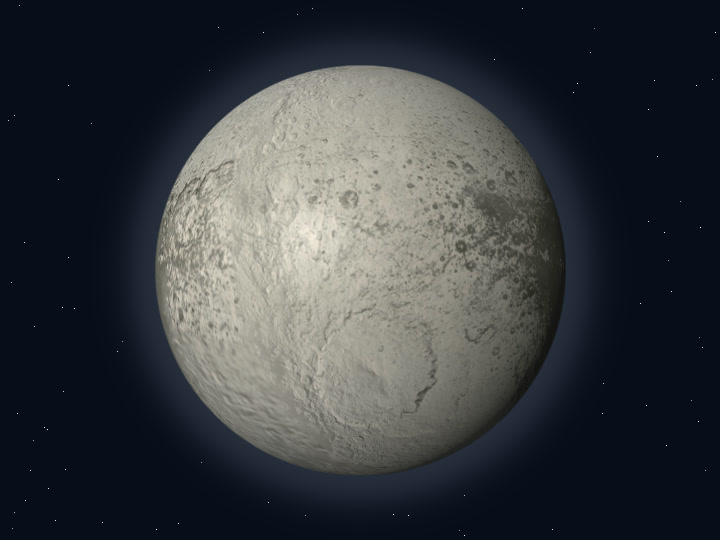
\includegraphics[width=\linewidth,height=4.4cm,keepaspectratio]{imagini/globuri/iapetus.jpg}\\[2pt]
{\scriptsize\itshape\color{orbitarMuted} Vedere 3D a corpului ceresc (\textbf{Iapetus})}
&
\centering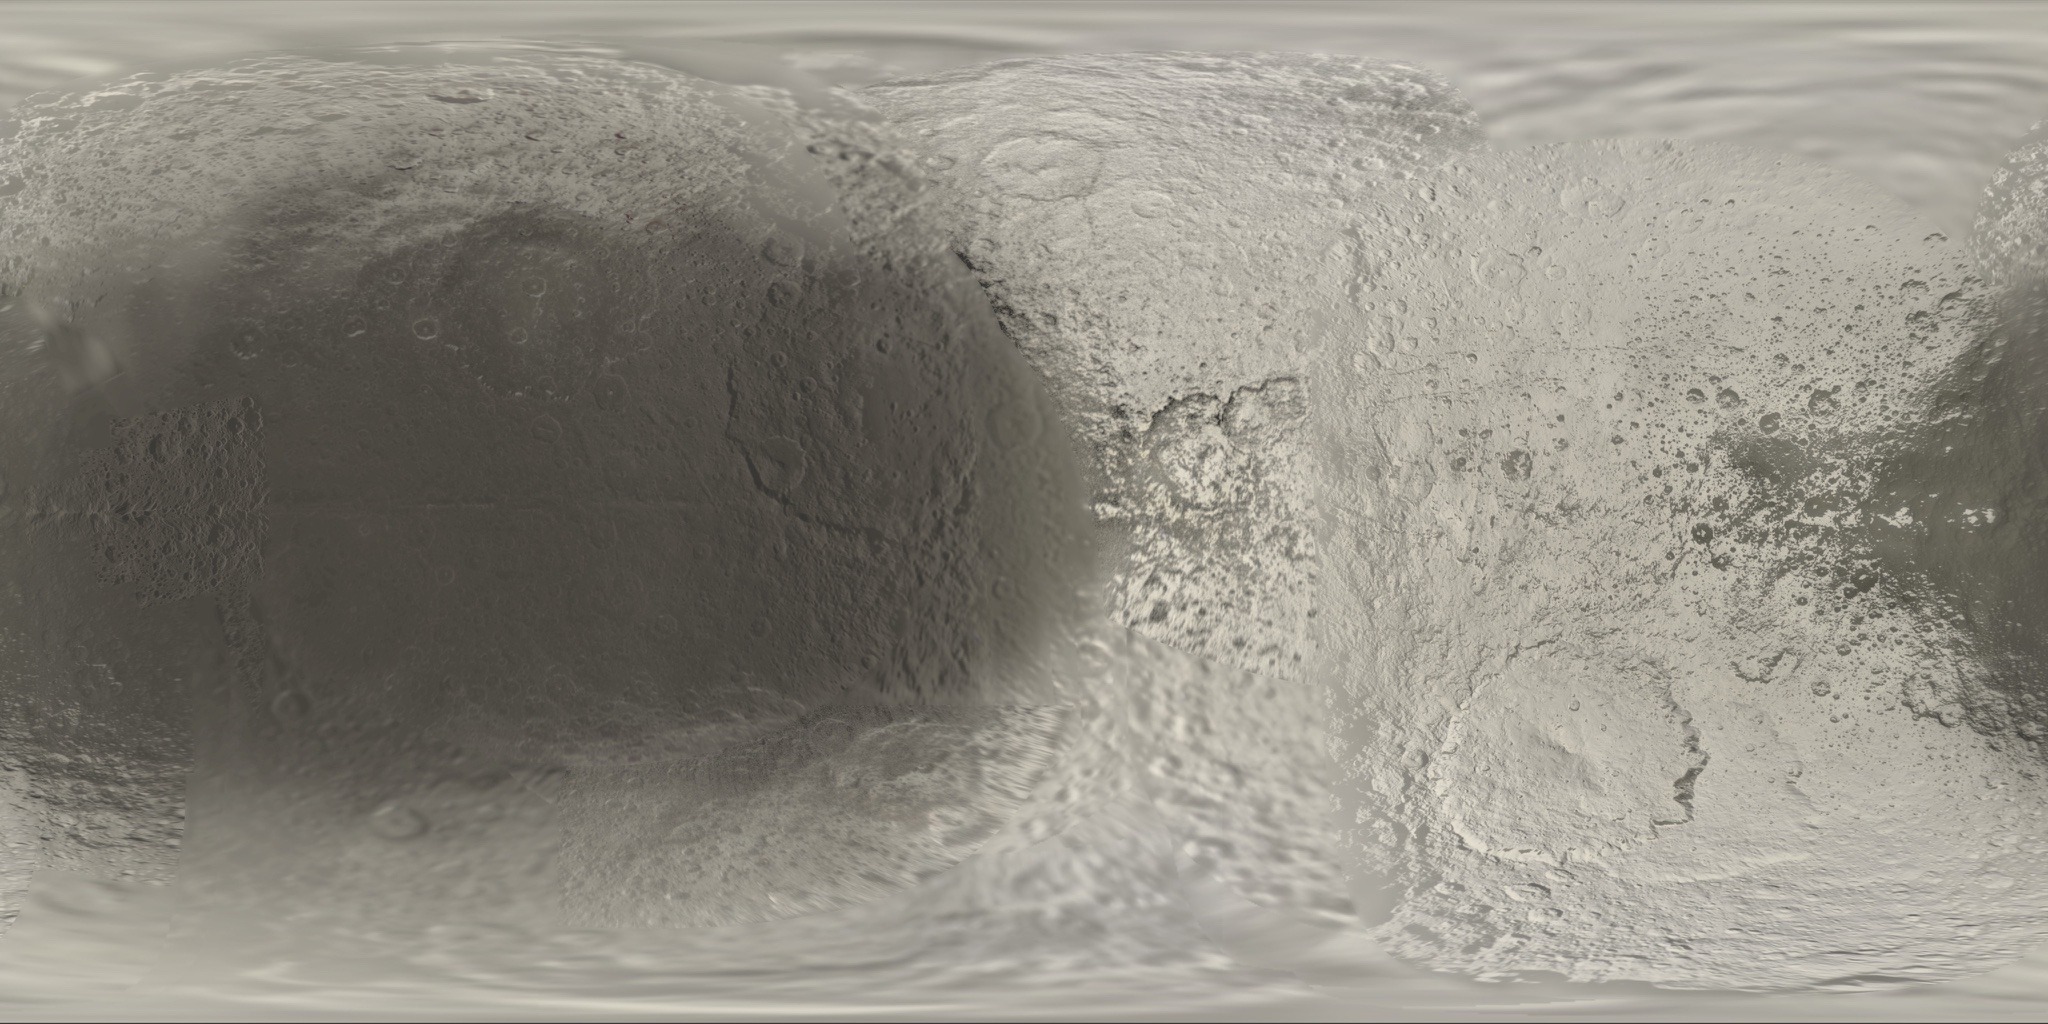
\includegraphics[width=\linewidth,height=4.4cm,keepaspectratio]{../public/textures/hd/iapetus_cassini.jpg}\\[2pt]
{\scriptsize\itshape\color{orbitarMuted} Planiglob desfășurat: Contrastul \quotedblbase{}Yin-Yang\textquotedblright{} dintre emisfera întunecată (Cassini Regio) și emisfera strălucitoare de gheață a lunii Iapetus (NASA/ESA Cassini).}
\end{tabular}
\end{center}


\begin{tcolorbox}[orbitardata, title={\textbf{Repere esențiale: Iapetus}}]
\small
\begin{itemize}[leftmargin=1.4em, itemsep=2pt, topsep=2pt]
  \item \textbf{Clasificare și orbită:} Satelit Natural (Lună) (orbitează în jurul: \textbf{Saturn}) \quad$\bullet$\quad \textbf{Distanță:} 9,582 UA ($\approx$ 1.433 milioane de kilometri)
  \item \textbf{Dimensiuni și masă:} rază medie 734,5 de kilometri \quad$\bullet$\quad masă: 3,00e-4 $\times M_\oplus$
  \item \textbf{Gravitație și regim termic:} 0,023 $\times g_\oplus$ (0,23 m/s$^2$) \quad$\bullet$\quad temperatură medie: -163 $^\circ$C (înclinarea axei: Nespecificată)
  \item \textbf{Ciclu orbital și rotație:} perioadă orbitală (an): 79,32 zile pământești \quad$\bullet$\quad rotație (zi): 1903,70 ore (79,32 zile pământești)
  \item \textbf{Durata călătoriei de pe Pământ:} cu viteza luminii ($1c$): \emph{1 oră și 11 minute}; cu racheta ($50.000$ de kilometri pe oră): \emph{7 ani}; cu avionul ($900$ de kilometri pe oră): \emph{160 de ani}; cu mașina ($100$ de kilometri pe oră): \emph{1.450 de ani}.
  \item \textbf{Repere de scară și curiozitate:} Datorită brâului de munți înalți care o înconjoară exact pe la mijloc, Iapetus seamănă cu o nucă uriașă în două culori! Munții de la ecuatorul lui Iapetus au 20 de kilometri înălțime, depășind de peste două ori înălțimea vârfului Everest de pe Pământ!
\end{itemize}
\end{tcolorbox}

\subsubsection*{Prezentare generală și profil astrofizic}
Descoperită de Giovanni Domenico Cassini în 1671, Iapetus este al treilea satelit ca mărime al lui Saturn. El a observat că satelitul este vizibil prin telescop doar pe o parte a orbitei sale, deducând corect că o emisferă este de 10 ori mai întunecată decât cealaltă. Iapetus este cea mai neobișnuită lună a lui Saturn: o jumătate din ea este neagră ca smoala, iar cealaltă jumătate este albă și strălucitoare ca zăpada! Datorită brâului de munți înalți care o înconjoară exact pe la mijloc, Iapetus seamănă cu o nucă uriașă în două culori!

\subsubsection*{Alcătuirea fizică și structura internă}
Privind în profunzimea sa, alcătuirea fizică este organizată pe mai multe straturi și regiuni distincte, fiecare având un rol bine definit în evoluția și dinamica acestui obiect cosmic. În primul rând se remarcă \textbf{Corp înghețat cu densitate mică (1,088 g/cm$^3$)}, compus în proporție de aproximativ 80\% din gheață de apă și aproximativ 20\% materiale stâncoase. În strânsă legătură cu această componentă se află \textbf{Emisfera întunecată (Cassini Regio) vs. Roncevaux Terra}, unde praful întunecat provenit de la satelitul exterior Phoebe absoarbe căldura solară și sublimează gheața către emisfera rece și albă. În completarea acestui ansamblu întâlnim \textbf{Creasta ecuatorială (1.300 de kilometri lungime)}, un lanț muntos lat de 20 de kilometri și înalt de până la 20 de kilometri care urmează perfect ecuatorul satelitului.

\subsubsection*{Observații astronomice și istoricul explorării}
Fotografiată de Voyager 2 în 1981 și survolată de aproape de sonda Cassini în septembrie 2007. Munții de la ecuatorul lui Iapetus au 20 de kilometri înălțime, depășind de peste două ori înălțimea vârfului Everest de pe Pământ!

\vspace{6pt}
\begin{tcolorbox}[orbitarquiz, title={\textbf{Întrebare de verificare \#22: Iapetus}}]
\textbf{Prin ce se remarcă vizual satelitul Iapetus al lui Saturn?}
\begin{itemize}[leftmargin=2.2em, itemsep=2pt, topsep=4pt]
  \item[$\square$ \textbf{A.}] Are o emisferă neagră ca cărbunele și una albă ca zăpada, plus o creastă muntoasă la ecuator
  \item[$\square$ \textbf{B.}] Este complet verde
  \item[$\square$ \textbf{C.}] Are trei inele proprii de foc
  \item[$\square$ \textbf{D.}] Este cel mai fierbinte corp din Sistemul Solar
\end{itemize}
\vspace{2pt}
{\footnotesize\color{orbitarMuted}\textbf{Răspuns corect:} \textbf{A} (Are o emisferă neagră ca cărbunele și una albă ca zăpada, plus o creastă muntoasă la ecuator). \emph{Iapetus prezintă cel mai dramatic contrast de culoare (albedo) din Sistemul Solar și o creastă ecuatorială care îi dă forma unei nuci.}}
\end{tcolorbox}
\clearpage


\subsection{Phoebe}
\label{sec:body-phoebe}
\vspace{-4pt}
{\large\itshape\color{orbitarAccent} Satelitul întunecat capturat din Centura Kuiper, cu orbită retrogradă în jurul lui Saturn}\\[4pt]


\begin{center}
\begin{tabular}{@{}m{0.44\textwidth}@{\hspace{0.03\textwidth}}m{0.51\textwidth}@{}}
\centering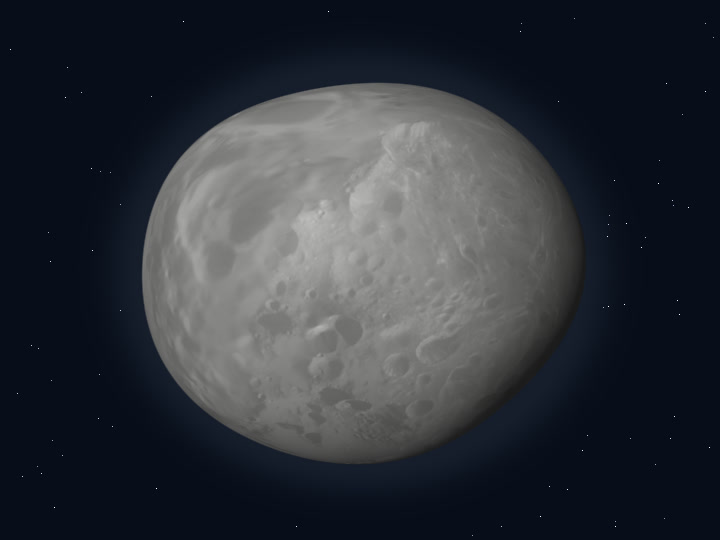
\includegraphics[width=\linewidth,height=4.4cm,keepaspectratio]{imagini/globuri/phoebe.jpg}\\[2pt]
{\scriptsize\itshape\color{orbitarMuted} Vedere 3D a corpului ceresc (\textbf{Phoebe})}
&
\centering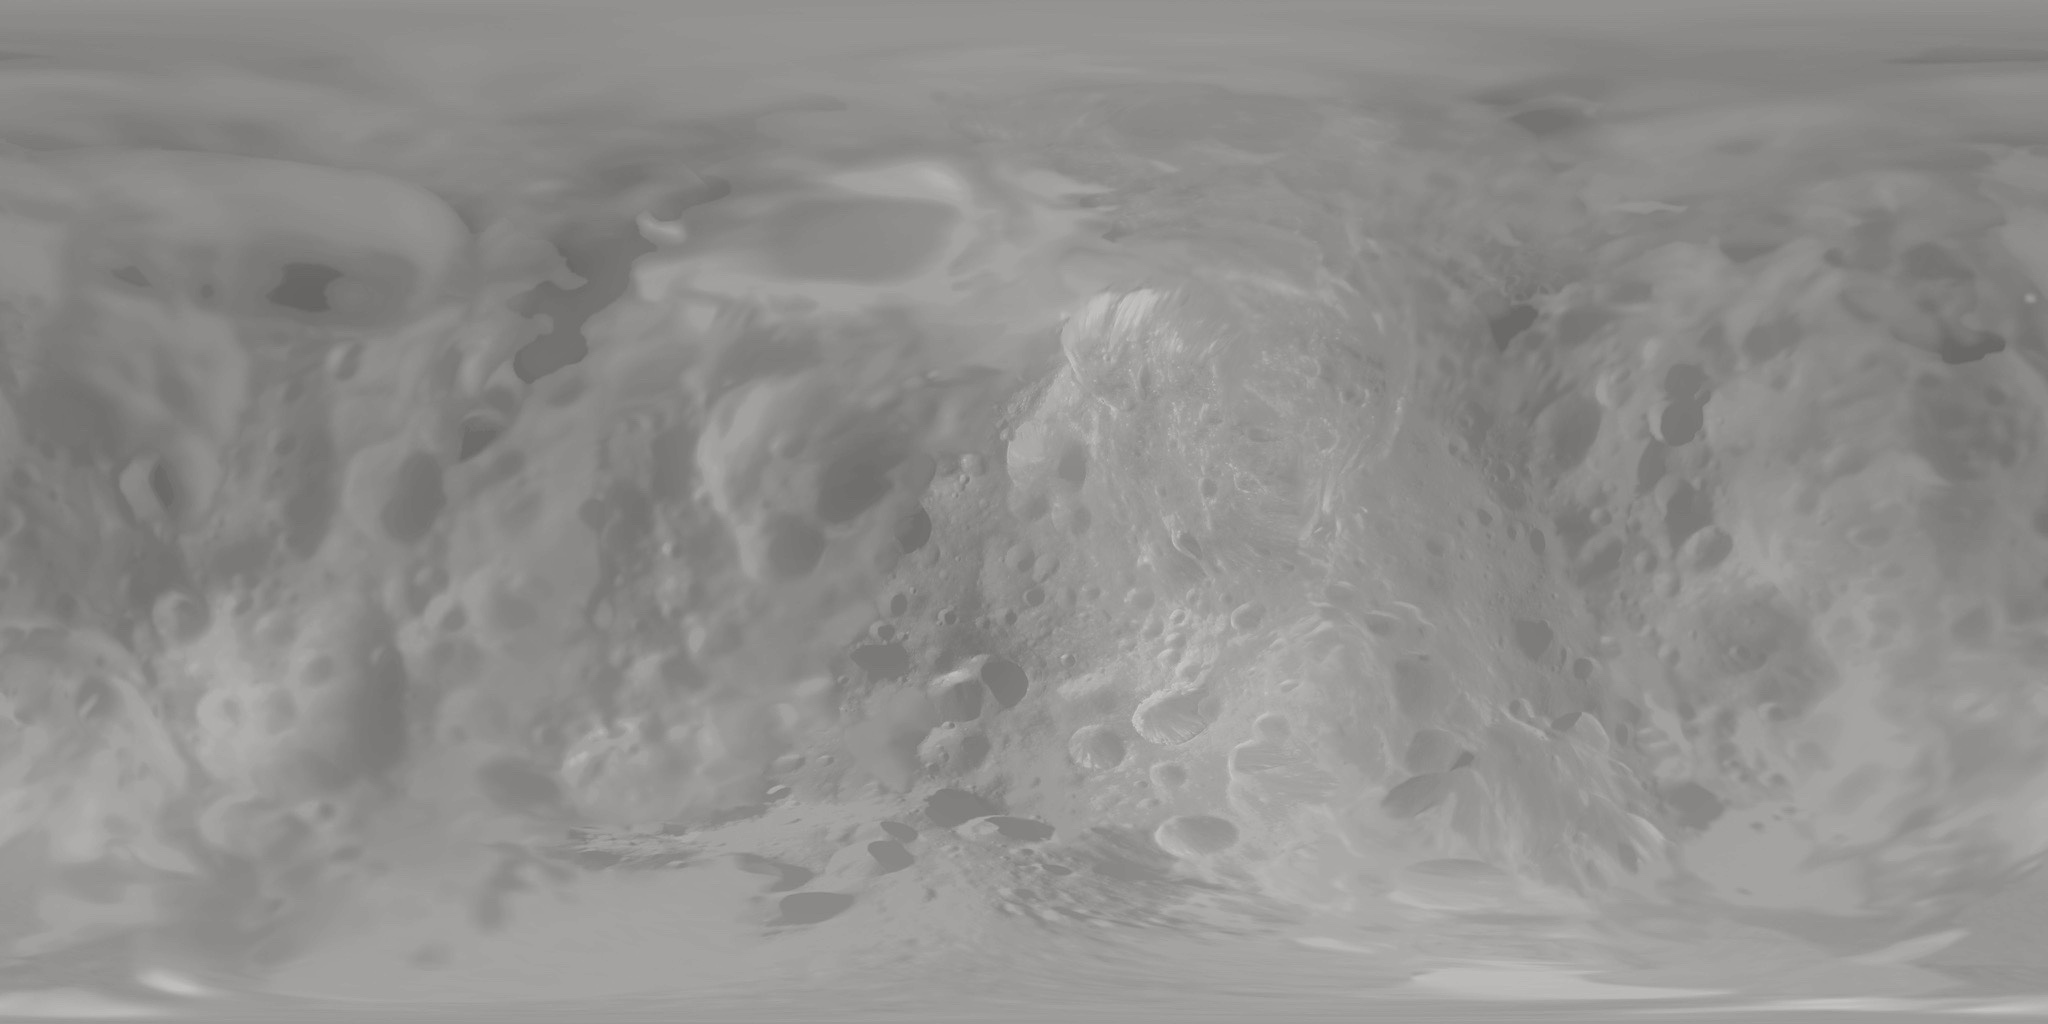
\includegraphics[width=\linewidth,height=4.4cm,keepaspectratio]{../public/textures/hd/phoebe_cassini.jpg}\\[2pt]
{\scriptsize\itshape\color{orbitarMuted} Planiglob desfășurat: Harta satelitului retrograd Phoebe (planetozimal capturat din Centura Kuiper) și a craterului Jason (NASA/ESA Cassini).}
\end{tabular}
\end{center}


\begin{tcolorbox}[orbitardata, title={\textbf{Repere esențiale: Phoebe}}]
\small
\begin{itemize}[leftmargin=1.4em, itemsep=2pt, topsep=2pt]
  \item \textbf{Clasificare și orbită:} Satelit Natural (Lună) (orbitează în jurul: \textbf{Saturn}) \quad$\bullet$\quad \textbf{Distanță:} 9,582 UA ($\approx$ 1.433 milioane de kilometri)
  \item \textbf{Dimensiuni și masă:} rază medie 106,5 kilometri \quad$\bullet$\quad masă: 1,39e-6 $\times M_\oplus$
  \item \textbf{Gravitație și regim termic:} 0,004 $\times g_\oplus$ (0,04 m/s$^2$) \quad$\bullet$\quad temperatură medie: -198 $^\circ$C (înclinarea axei: Nespecificată)
  \item \textbf{Ciclu orbital și rotație:} perioadă orbitală (an): 550,31 zile pământești (Orbită retrogradă!) \quad$\bullet$\quad rotație (zi): 9,27 ore (0,39 zile pământești)
  \item \textbf{Durata călătoriei de pe Pământ:} cu viteza luminii ($1c$): \emph{1 oră și 11 minute}; cu racheta ($50.000$ de kilometri pe oră): \emph{7 ani}; cu avionul ($900$ de kilometri pe oră): \emph{160 de ani}; cu mașina ($100$ de kilometri pe oră): \emph{1.450 de ani}.
  \item \textbf{Repere de scară și curiozitate:} La fel ca Triton la Neptun, Phoebe zboară \guillemotleft{}pe contrasens\guillemotright{} în jurul lui Saturn, la o distanță uriașă de aproape 13 milioane de kilometri! Phoebe a fost primul satelit descoperit vreodată cu ajutorul fotografiilor astronomice, în anul 1899, și lasă în urma lui cel mai mare inel de praf al lui Saturn!
\end{itemize}
\end{tcolorbox}

\subsubsection*{Prezentare generală și profil astrofizic}
Descoperită în 1899 de William Henry Pickering pe plăci fotografice, Phoebe (diametru mediu 213 kilometri) orbitează retrograd la 12,9 milioane de kilometri de Saturn în 550 de zile. Densitatea ridicată (1,63 g/cm$^3$) și compoziția isotopică arată că este un centaur primordial capturat din Centura Kuiper. Phoebe este un călător misterios de la marginea Sistemului Solar care a fost prins de gravitația lui Saturn! Este negru ca cărbunele la exterior, dar ascunde gheață albă sub praf. La fel ca Triton la Neptun, Phoebe zboară \guillemotleft{}pe contrasens\guillemotright{} în jurul lui Saturn, la o distanță uriașă de aproape 13 milioane de kilometri!

\subsubsection*{Alcătuirea fizică și structura internă}
Privind în profunzimea sa, alcătuirea fizică este organizată pe mai multe straturi și regiuni distincte, fiecare având un rol bine definit în evoluția și dinamica acestui obiect cosmic. În primul rând se remarcă \textbf{Interior dens de rocă și gheață (1,63 g/cm$^3$)}, compoziție similară cu cea a lui Pluto și Triton, mult mai bogată în rocă decât lunile interioare ale lui Saturn. În strânsă legătură cu această componentă se află \textbf{Craterul gigant Jason (101 kilometri diametru)}, impacturile meteoritice au îndepărtat pătura neagră de compuși organici și filosilicați, dezvăluind pereți strălucitori de gheață de apă. În completarea acestui ansamblu întâlnim \textbf{Sursa gigantului \guillemotleft{}Inel Phoebe\guillemotright{}}, micrometeoriții lovesc continuu Phoebe și ridică un inel vast de praf întunecat care cade în spirală și înnegrește emisfera anterioară a lui Iapetus.

\subsubsection*{Observații astronomice și istoricul explorării}
A fost prima țintă studiată de sonda Cassini la sosirea în sistemul lui Saturn, printr-un survol la 2.068 de kilometri distanță pe 11 iunie 2004. Phoebe a fost primul satelit descoperit vreodată cu ajutorul fotografiilor astronomice, în anul 1899, și lasă în urma lui cel mai mare inel de praf al lui Saturn!

\vspace{6pt}
\begin{tcolorbox}[orbitarquiz, title={\textbf{Întrebare de verificare \#23: Phoebe}}]
\textbf{Care este originea satelitului exterior Phoebe al lui Saturn și ce efect produce praful desprins de pe el?}
\begin{itemize}[leftmargin=2.2em, itemsep=2pt, topsep=4pt]
  \item[$\square$ \textbf{A.}] Este un corp capturat din Centura Kuiper, iar praful său întunecat colorează în negru o emisferă a satelitului Iapetus
  \item[$\square$ \textbf{B.}] Este o bucată din Soare
  \item[$\square$ \textbf{C.}] Este făcut din gaz hidrogen
  \item[$\square$ \textbf{D.}] Orbitează în interiorul inelelor principale
\end{itemize}
\vspace{2pt}
{\footnotesize\color{orbitarMuted}\textbf{Răspuns corect:} \textbf{A} (Este un corp capturat din Centura Kuiper, iar praful său întunecat colorează în negru o emisferă a satelitului Iapetus). \emph{Orbita retrogradă și compoziția lui Phoebe confirmă că a fost capturat din Centura Kuiper, iar praful din Inelul Phoebe este responsabil pentru emisfera întunecată a lui Iapetus.}}
\end{tcolorbox}
\clearpage


\section{Uranus}
\label{sec:body-uranus}
\vspace{-4pt}
{\large\itshape\color{orbitarAccent} Gigantul de gheață turcoaz care se rostogolește pe orbită}\\[4pt]


\begin{center}
\begin{tabular}{@{}m{0.44\textwidth}@{\hspace{0.03\textwidth}}m{0.51\textwidth}@{}}
\centering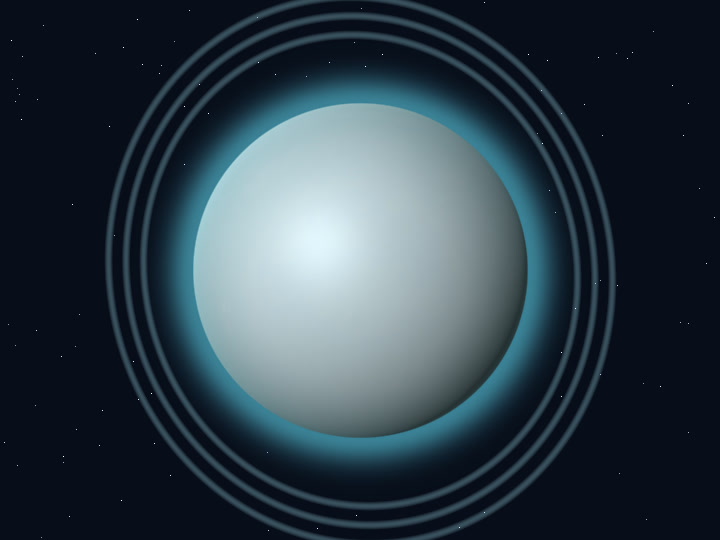
\includegraphics[width=\linewidth,height=4.4cm,keepaspectratio]{imagini/globuri/uranus.jpg}\\[2pt]
{\scriptsize\itshape\color{orbitarMuted} Vedere 3D a corpului ceresc (\textbf{Uranus})}
&
\centering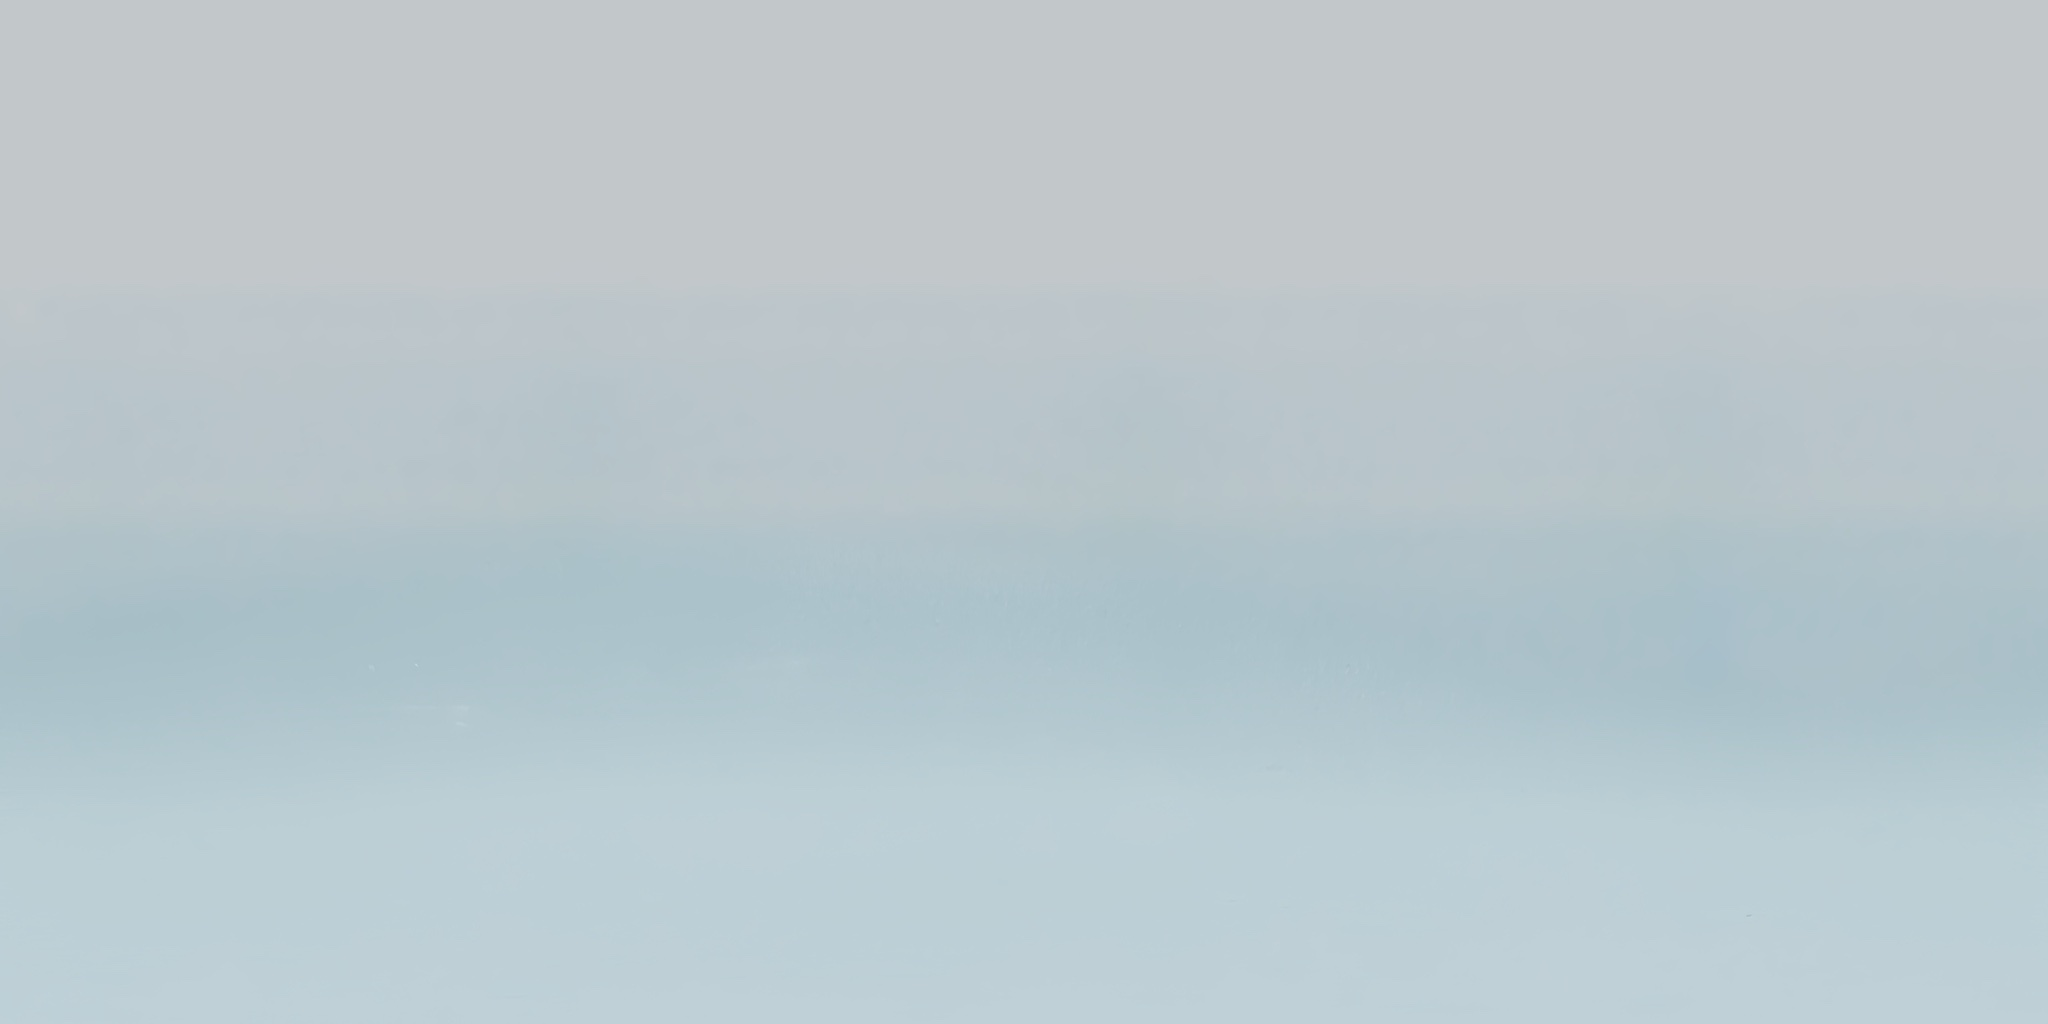
\includegraphics[width=\linewidth,height=4.4cm,keepaspectratio]{../public/textures/hd/uranus_voyager.jpg}\\[2pt]
{\scriptsize\itshape\color{orbitarMuted} Planiglob desfășurat: Harta atmosferei de hidrogen, heliu și metan a gigantului de gheață Uranus (date NASA Voyager 2).}
\end{tabular}
\end{center}


\begin{tcolorbox}[orbitardata, title={\textbf{Repere esențiale: Uranus}}]
\small
\begin{itemize}[leftmargin=1.4em, itemsep=2pt, topsep=2pt]
  \item \textbf{Clasificare și orbită:} Gigant de Gheață \quad$\bullet$\quad \textbf{Distanță:} 19,218 UA ($\approx$ 2.875 milioane de kilometri)
  \item \textbf{Dimensiuni și masă:} rază medie 25.362 de kilometri \quad$\bullet$\quad masă: 14,540 $\times M_\oplus$
  \item \textbf{Gravitație și regim termic:} 0,890 $\times g_\oplus$ (8,73 m/s$^2$) \quad$\bullet$\quad temperatură medie: -195 $^\circ$C (înclinarea axei: 97,77$^\circ$)
  \item \textbf{Ciclu orbital și rotație:} perioadă orbitală (an): 30.688,5 zile ($\approx$ 84,02 ani pământești) \quad$\bullet$\quad rotație (zi): 17,24 ore (Rotație retrogradă!)
  \item \textbf{Durata călătoriei de pe Pământ:} cu viteza luminii ($1c$): \emph{2 ore și 30 de minute}; cu racheta ($50.000$ de kilometri pe oră): \emph{8 ani și jumătate}; cu avionul ($900$ de kilometri pe oră): \emph{345 de ani}; cu mașina ($100$ de kilometri pe oră): \emph{3.100 de ani}.
  \item \textbf{Repere de scară și curiozitate:} Dacă Pământul e o mărgea, Uranus e cât un măr mare de culoarea gheții! Un anotimp pe Uranus durează 21 de ani pământești de lumină continuă sau de întuneric!
\end{itemize}
\end{tcolorbox}

\subsubsection*{Prezentare generală și profil astrofizic}
Prima planetă descoperită cu ajutorul telescopului (William Herschel, 1781), Uranus este clasificată drept \guillemotleft{}gigant de gheață\guillemotright{}. Înclinarea axială extremă de 97,77$^\circ$ este atribuită unei coliziuni cataclismice cu o protoplanetă în tinerețea Sistemului Solar. Uranus este o planetă de culoare bleu-turcoaz care face ceva unic: în loc să se învârtă ca un titirez drept, stă culcată pe o parte și se rostogolește ca o minge! Dacă Pământul e o mărgea, Uranus e cât un măr mare de culoarea gheții!

\subsubsection*{Alcătuirea fizică și structura internă}
Privind în profunzimea sa, alcătuirea fizică este organizată pe mai multe straturi și regiuni distincte, fiecare având un rol bine definit în evoluția și dinamica acestui obiect cosmic. În primul rând se remarcă \textbf{Nucleu silicat-metalic rece}, de dimensiuni relativ reduse, emițând foarte puțină căldură internă. În strânsă legătură cu această componentă se află \textbf{Manta fluidă de \guillemotleft{}ghețuri\guillemotright{}}, amestec dens și fierbinte de apă, amoniac și metan aflate la presiuni extreme. În completarea acestui ansamblu întâlnim \textbf{Atmosferă de hidrogen, heliu și metan}, unde metanul absoarbe lumina roșie a Soarelui și reflectă nuanța caracteristică cyan.

\subsubsection*{Observații astronomice și istoricul explorării}
Descoperită în 1781 și vizitată de o singură navă spațială până în prezent: Voyager 2 în ianuarie 1986. Un anotimp pe Uranus durează 21 de ani pământești de lumină continuă sau de întuneric!

\vspace{6pt}
\begin{tcolorbox}[orbitarquiz, title={\textbf{Întrebare de verificare \#24: Uranus}}]
\textbf{Ce gaz din atmosfera lui Uranus îi oferă culoarea turcoaz (cyan)?}
\begin{itemize}[leftmargin=2.2em, itemsep=2pt, topsep=4pt]
  \item[$\square$ \textbf{A.}] Oxigenul
  \item[$\square$ \textbf{B.}] Dioxidul de carbon
  \item[$\square$ \textbf{C.}] Metanul
  \item[$\square$ \textbf{D.}] Azotul
\end{itemize}
\vspace{2pt}
{\footnotesize\color{orbitarMuted}\textbf{Răspuns corect:} \textbf{C} (Metanul). \emph{Metanul (CH$_4$) din atmosfera superioară absoarbe componenta roșie a luminii solare și difuzează lumina albastră-verzuie.}}
\end{tcolorbox}
\clearpage


\subsection{Miranda}
\label{sec:body-miranda}
\vspace{-4pt}
{\large\itshape\color{orbitarAccent} Luna-puzzle a lui Uranus, cu cea mai înaltă stâncă din Sistemul Solar}\\[4pt]


\begin{center}
\begin{tabular}{@{}m{0.44\textwidth}@{\hspace{0.03\textwidth}}m{0.51\textwidth}@{}}
\centering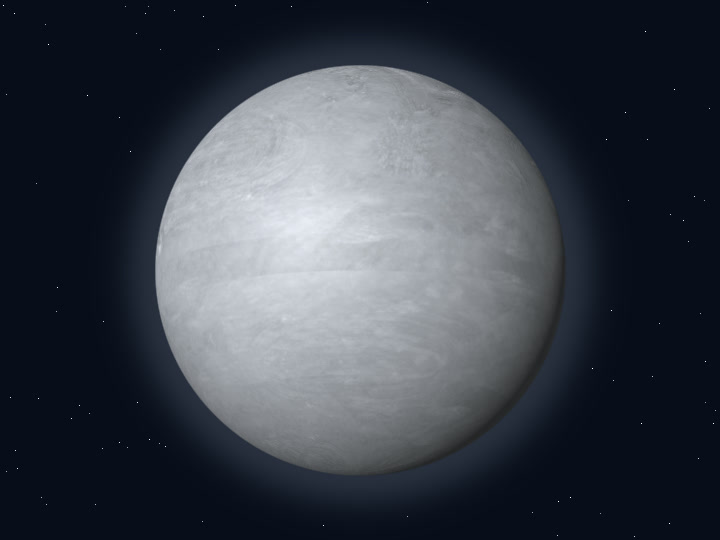
\includegraphics[width=\linewidth,height=4.4cm,keepaspectratio]{imagini/globuri/miranda.jpg}\\[2pt]
{\scriptsize\itshape\color{orbitarMuted} Vedere 3D a corpului ceresc (\textbf{Miranda})}
&
\centering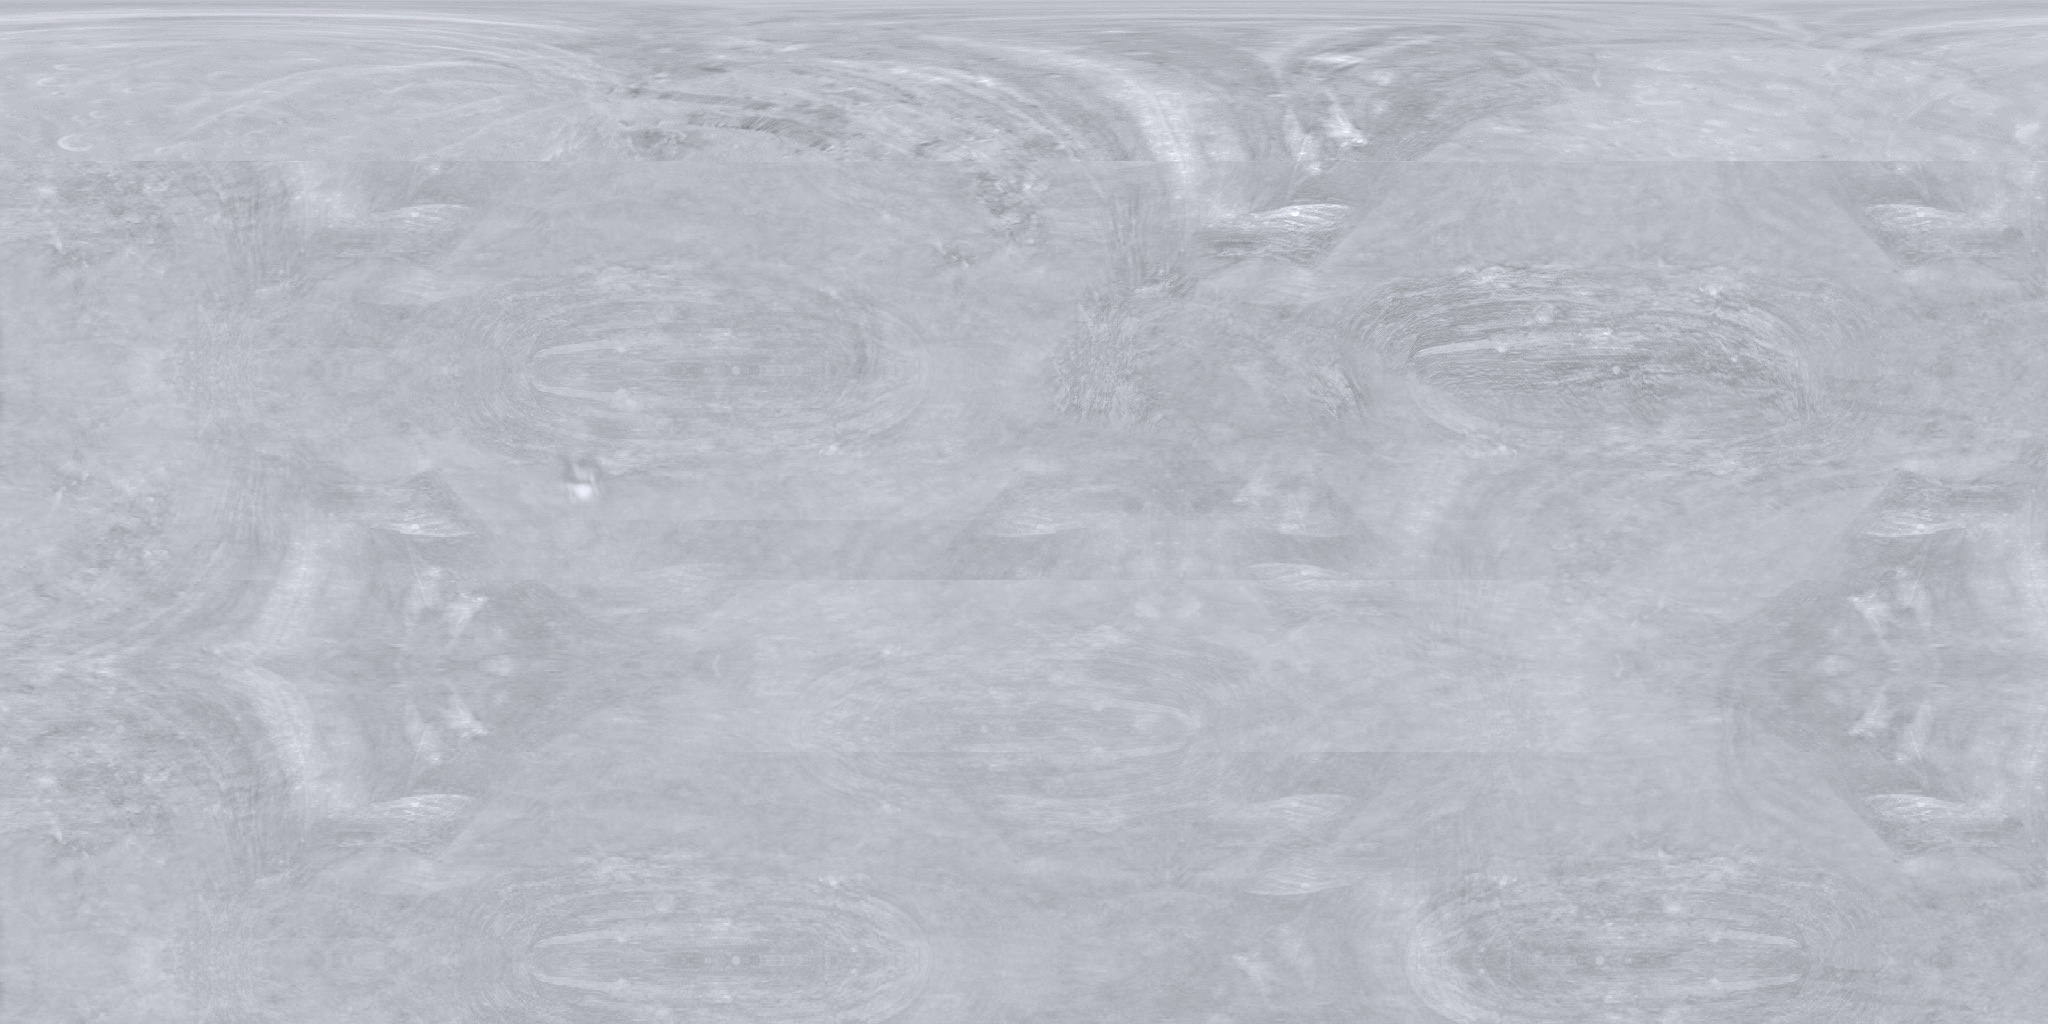
\includegraphics[width=\linewidth,height=4.4cm,keepaspectratio]{../public/textures/hd/miranda_voyager.jpg}\\[2pt]
{\scriptsize\itshape\color{orbitarMuted} Planiglob desfășurat: Relieful spectaculos al lunii Miranda, cu stâncile Verona Rupes și regiunile coronae (NASA Voyager 2).}
\end{tabular}
\end{center}


\begin{tcolorbox}[orbitardata, title={\textbf{Repere esențiale: Miranda}}]
\small
\begin{itemize}[leftmargin=1.4em, itemsep=2pt, topsep=2pt]
  \item \textbf{Clasificare și orbită:} Satelit Natural (Lună) (orbitează în jurul: \textbf{Uranus}) \quad$\bullet$\quad \textbf{Distanță:} 19,218 UA ($\approx$ 2.875 milioane de kilometri)
  \item \textbf{Dimensiuni și masă:} rază medie 235,8 de kilometri \quad$\bullet$\quad masă: 1,10e-5 $\times M_\oplus$
  \item \textbf{Gravitație și regim termic:} 0,008 $\times g_\oplus$ (0,08 m/s$^2$) \quad$\bullet$\quad temperatură medie: -213 $^\circ$C (înclinarea axei: Nespecificată)
  \item \textbf{Ciclu orbital și rotație:} perioadă orbitală (an): 1,413 zile pământești \quad$\bullet$\quad rotație (zi): 33,90 ore (1,41 zile pământești)
  \item \textbf{Durata călătoriei de pe Pământ:} cu viteza luminii ($1c$): \emph{2 ore și 30 de minute}; cu racheta ($50.000$ de kilometri pe oră): \emph{8 ani și jumătate}; cu avionul ($900$ de kilometri pe oră): \emph{345 de ani}; cu mașina ($100$ de kilometri pe oră): \emph{3.100 de ani}.
  \item \textbf{Repere de scară și curiozitate:} Pe Miranda se află Verona Rupes, o prăpastie de gheață atât de înaltă încât, dacă ai sări de pe marginea ei, ai pluti în cădere timp de 12 minute până jos! Stânca Verona Rupes are 20 de kilometri înălțime și este cea mai înaltă prăpastie din întregul Sistem Solar!
\end{itemize}
\end{tcolorbox}

\subsubsection*{Prezentare generală și profil astrofizic}
Descoperită de Gerard Kuiper în 1948, Miranda este cea mai interioară și mai mică dintre cele cinci luni majore ale lui Uranus. Suprafața ei prezintă cel mai extrem relief tectonic raportat la dimensiunea sa, cu canioane de 12 ori mai adânci decât Marele Canion. Miranda este o lună mică și uimitoare a lui Uranus, care arată de parcă a fost lipită la loc din piese diferite de puzzle de gheață! Pe Miranda se află Verona Rupes, o prăpastie de gheață atât de înaltă încât, dacă ai sări de pe marginea ei, ai pluti în cădere timp de 12 minute până jos!

\subsubsection*{Alcătuirea fizică și structura internă}
Privind în profunzimea sa, alcătuirea fizică este organizată pe mai multe straturi și regiuni distincte, fiecare având un rol bine definit în evoluția și dinamica acestui obiect cosmic. În primul rând se remarcă \textbf{Nucleu de silicați și manta de gheață}, încălzită în trecut de rezonanțe orbitale cu ceilalți sateliți ai lui Uranus. În strânsă legătură cu această componentă se află \textbf{Coronae (Inverness, Arden, Elsinore)}, trei regiuni poligonale uriașe (peste 200 de kilometri lățime) cu creste și șanțuri concentrice în formă de chevron. În completarea acestui ansamblu întâlnim \textbf{Verona Rupes}, falie tectonică verticală de gheață cu o înălțime estimată la 20 de kilometri.

\subsubsection*{Observații astronomice și istoricul explorării}
Survolată de aproape de sonda Voyager 2 la 24 ianuarie 1986, care a transmis singurele imagini detaliate ale suprafeței sale. Stânca Verona Rupes are 20 de kilometri înălțime și este cea mai înaltă prăpastie din întregul Sistem Solar!

\vspace{6pt}
\begin{tcolorbox}[orbitarquiz, title={\textbf{Întrebare de verificare \#25: Miranda}}]
\textbf{Ce record deține stânca Verona Rupes de pe satelitul Miranda al lui Uranus?}
\begin{itemize}[leftmargin=2.2em, itemsep=2pt, topsep=4pt]
  \item[$\square$ \textbf{A.}] Este cel mai fierbinte vulcan
  \item[$\square$ \textbf{B.}] Este cea mai înaltă faleză (prăpastie) cunoscută din Sistemul Solar (aproximativ 20 de kilometri înălțime)
  \item[$\square$ \textbf{C.}] Este cel mai adânc ocean
  \item[$\square$ \textbf{D.}] Este cel mai lung râu de metan
\end{itemize}
\vspace{2pt}
{\footnotesize\color{orbitarMuted}\textbf{Răspuns corect:} \textbf{B} (Este cea mai înaltă faleză (prăpastie) cunoscută din Sistemul Solar (aproximativ 20 de kilometri înălțime)). \emph{Verona Rupes se ridică la aproximativ 20 de kilometri deasupra terenului înconjurător, fiind de peste două ori mai înaltă decât muntele Everest.}}
\end{tcolorbox}
\clearpage


\subsection{Ariel}
\label{sec:body-ariel}
\vspace{-4pt}
{\large\itshape\color{orbitarAccent} Cea mai luminoasă lună a lui Uranus, străbătută de văi tectonice și câmpii netede}\\[4pt]


\begin{center}
\begin{tabular}{@{}m{0.44\textwidth}@{\hspace{0.03\textwidth}}m{0.51\textwidth}@{}}
\centering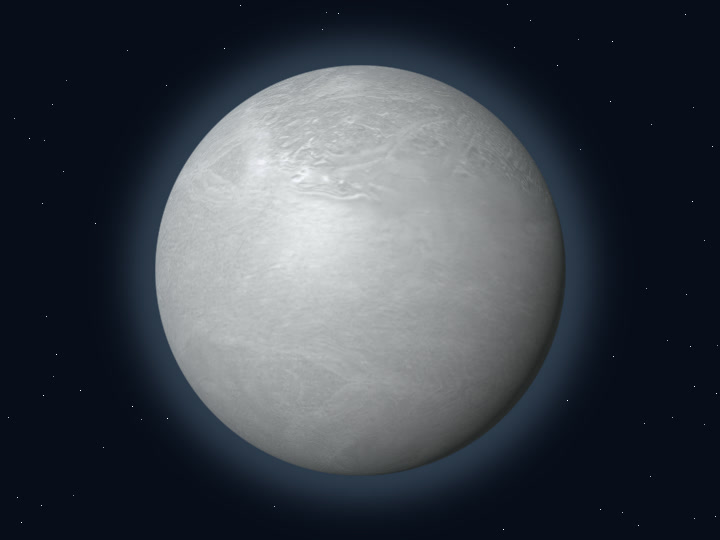
\includegraphics[width=\linewidth,height=4.4cm,keepaspectratio]{imagini/globuri/ariel.jpg}\\[2pt]
{\scriptsize\itshape\color{orbitarMuted} Vedere 3D a corpului ceresc (\textbf{Ariel})}
&
\centering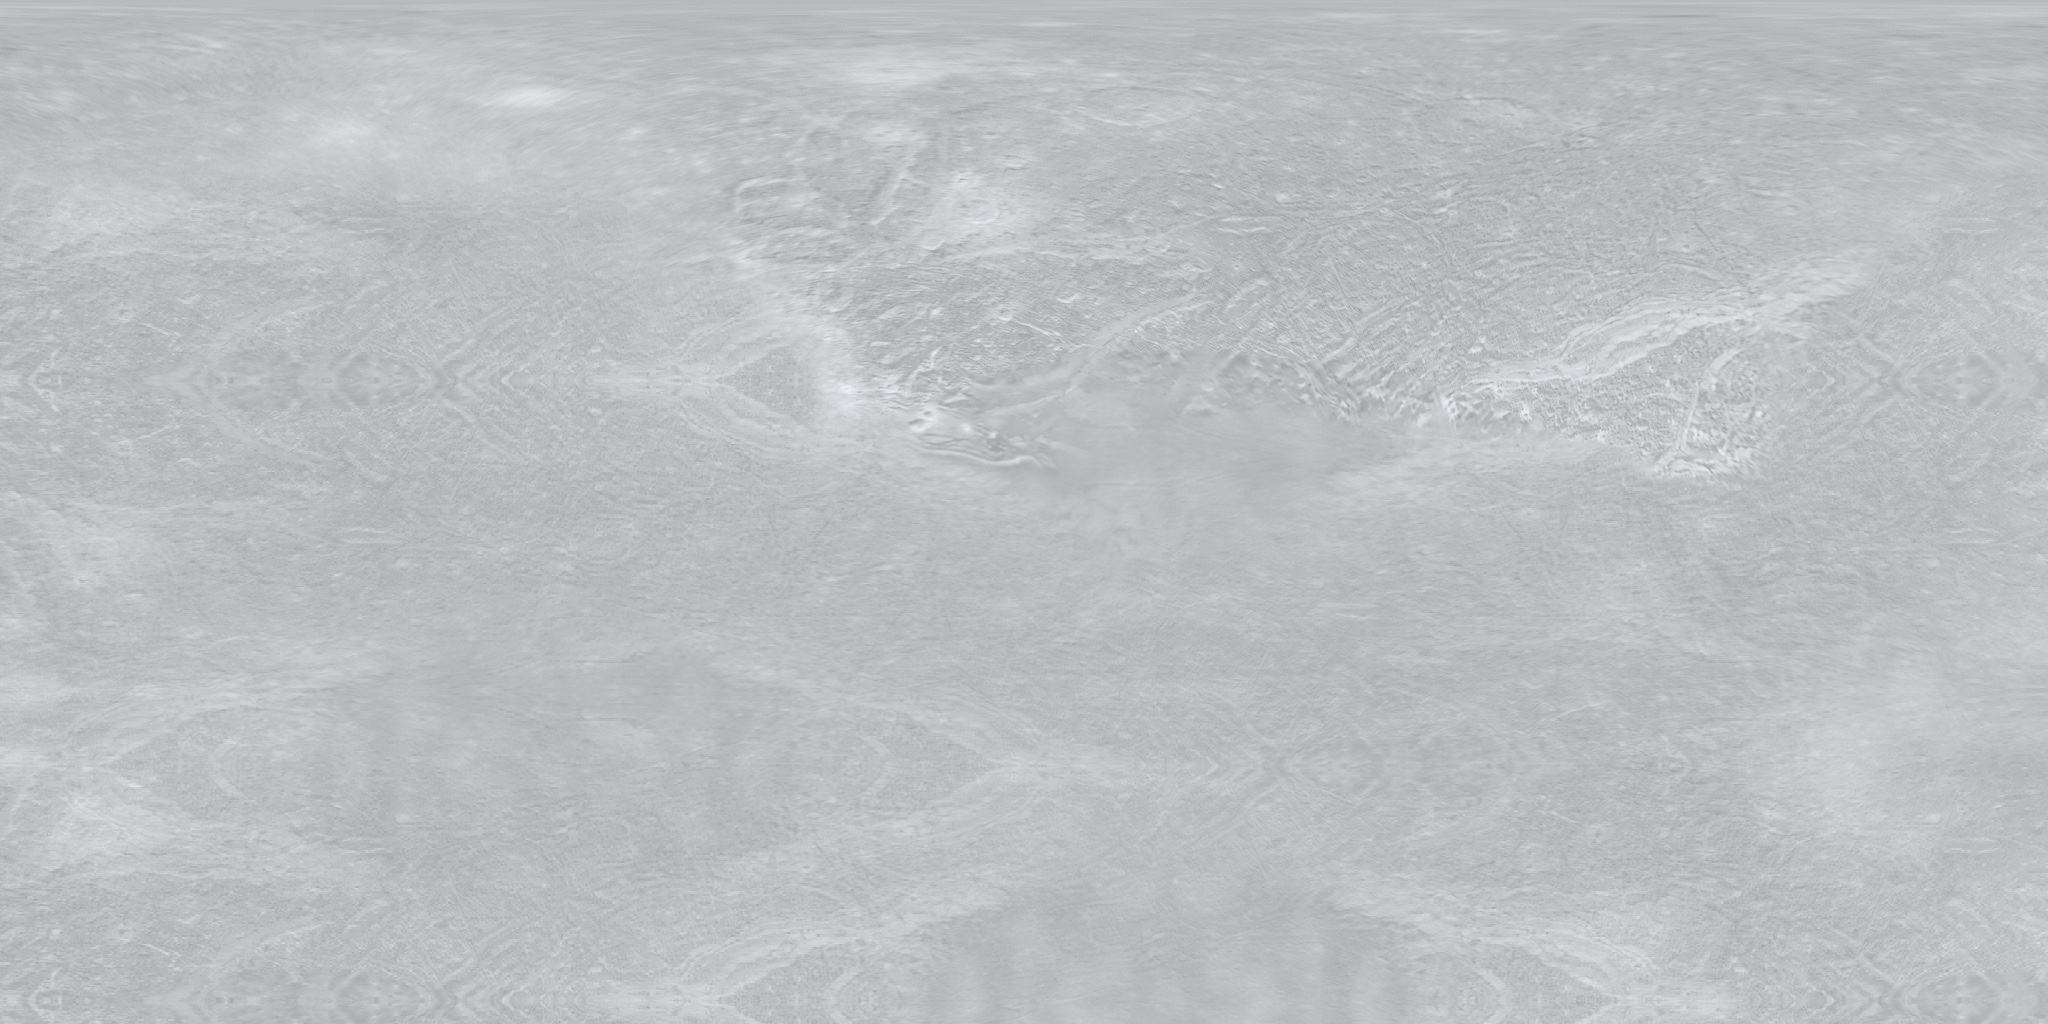
\includegraphics[width=\linewidth,height=4.4cm,keepaspectratio]{../public/textures/hd/ariel_voyager.jpg}\\[2pt]
{\scriptsize\itshape\color{orbitarMuted} Planiglob desfășurat: Harta celei mai luminoase luni a lui Uranus, Ariel, brăzdată de canioanele tectonice Kachina Chasmata (NASA Voyager 2).}
\end{tabular}
\end{center}


\begin{tcolorbox}[orbitardata, title={\textbf{Repere esențiale: Ariel}}]
\small
\begin{itemize}[leftmargin=1.4em, itemsep=2pt, topsep=2pt]
  \item \textbf{Clasificare și orbită:} Satelit Natural (Lună) (orbitează în jurul: \textbf{Uranus}) \quad$\bullet$\quad \textbf{Distanță:} 19,218 UA ($\approx$ 2.875 milioane de kilometri)
  \item \textbf{Dimensiuni și masă:} rază medie 578,9 de kilometri \quad$\bullet$\quad masă: 2,09e-4 $\times M_\oplus$
  \item \textbf{Gravitație și regim termic:} 0,025 $\times g_\oplus$ (0,25 m/s$^2$) \quad$\bullet$\quad temperatură medie: -213 $^\circ$C (înclinarea axei: Nespecificată)
  \item \textbf{Ciclu orbital și rotație:} perioadă orbitală (an): 2,52 zile pământești \quad$\bullet$\quad rotație (zi): 60,49 ore (2,52 zile pământești)
  \item \textbf{Durata călătoriei de pe Pământ:} cu viteza luminii ($1c$): \emph{2 ore și 30 de minute}; cu racheta ($50.000$ de kilometri pe oră): \emph{8 ani și jumătate}; cu avionul ($900$ de kilometri pe oră): \emph{345 de ani}; cu mașina ($100$ de kilometri pe oră): \emph{3.100 de ani}.
  \item \textbf{Repere de scară și curiozitate:} Ariel poartă numele unui spirit jucăuș al aerului din piesa \guillemotleft{}Furtuna\guillemotright{} de William Shakespeare! Telescopul Spațial James Webb a descoperit pe Ariel gheață de dioxid de carbon care pare să fi ieșit chiar din interiorul lunii!
\end{itemize}
\end{tcolorbox}

\subsubsection*{Prezentare generală și profil astrofizic}
Descoperită în 1851 de William Lassell, Ariel are cea mai tânără și mai activă suprafață geologică dintre sateliții lui Uranus (după Miranda), cu un albedo ridicat (0,39) și o rețea vastă de grabene tectonice (Kachina Chasmata) și câmpii criovulcanice. Ariel este cea mai strălucitoare dintre cele cinci luni mari ale lui Uranus! Suprafața ei este brăzdată de canioane lungi și largi, cu podele netede ca niște autostrăzi de gheață. Ariel poartă numele unui spirit jucăuș al aerului din piesa \guillemotleft{}Furtuna\guillemotright{} de William Shakespeare!

\subsubsection*{Alcătuirea fizică și structura internă}
Privind în profunzimea sa, alcătuirea fizică este organizată pe mai multe straturi și regiuni distincte, fiecare având un rol bine definit în evoluția și dinamica acestui obiect cosmic. În primul rând se remarcă \textbf{Nucleu diferențiat de rocă (aproximativ 50\%) și manta de gheață (aproximativ 50\%)}, densitate medie de 1,59 g/cm$^3$, cu indicii puternice privind existența unui ocean subteran rezidual. În strânsă legătură cu această componentă se află \textbf{Sistemul de canioane Kachina Chasmata}, grabene tectonice lungi de peste 620 de kilometri și adânci de 5--10 kilometri, ale căror podele au fost netezite de curgeri criovulcanice de gheață de apă și amoniac. În completarea acestui ansamblu întâlnim \textbf{Depozite de dioxid de carbon (CO$_2$) și monoxid de carbon}, detectate în 2023--2024 de Telescopul James Webb pe emisfera posterioară, sugerând procese de degazare din interior.

\subsubsection*{Observații astronomice și istoricul explorării}
Fotografiată de sonda Voyager 2 în ianuarie 1986 (de la 127.000 de kilometri distanță) și analizată spectroscopic de Telescopul Spațial James Webb. Telescopul Spațial James Webb a descoperit pe Ariel gheață de dioxid de carbon care pare să fi ieșit chiar din interiorul lunii!

\vspace{6pt}
\begin{tcolorbox}[orbitarquiz, title={\textbf{Întrebare de verificare \#26: Ariel}}]
\textbf{Prin ce se distinge suprafața satelitului Ariel față de vecina sa întunecată Umbriel?}
\begin{itemize}[leftmargin=2.2em, itemsep=2pt, topsep=4pt]
  \item[$\square$ \textbf{A.}] Ariel este cea mai luminoasă lună a lui Uranus și are o suprafață tânără, tăiată de canioane tectonice (Kachina Chasmata) și câmpii criovulcanice
  \item[$\square$ \textbf{B.}] Ariel este acoperită cu păduri
  \item[$\square$ \textbf{C.}] Ariel nu are niciun crater sau vale
  \item[$\square$ \textbf{D.}] Ariel este făcută din fier lichid
\end{itemize}
\vspace{2pt}
{\footnotesize\color{orbitarMuted}\textbf{Răspuns corect:} \textbf{A} (Ariel este cea mai luminoasă lună a lui Uranus și are o suprafață tânără, tăiată de canioane tectonice (Kachina Chasmata) și câmpii criovulcanice). \emph{Încălzirea mareică din trecut a remodelat suprafața lui Ariel prin falii tectonice și criovulcanism, făcând-o cea mai strălucitoare lună a lui Uranus.}}
\end{tcolorbox}
\clearpage


\subsection{Umbriel}
\label{sec:body-umbriel}
\vspace{-4pt}
{\large\itshape\color{orbitarAccent} Luna întunecată a lui Uranus, cu misteriosul inel luminos al craterului Wunda}\\[4pt]


\begin{center}
\begin{tabular}{@{}m{0.44\textwidth}@{\hspace{0.03\textwidth}}m{0.51\textwidth}@{}}
\centering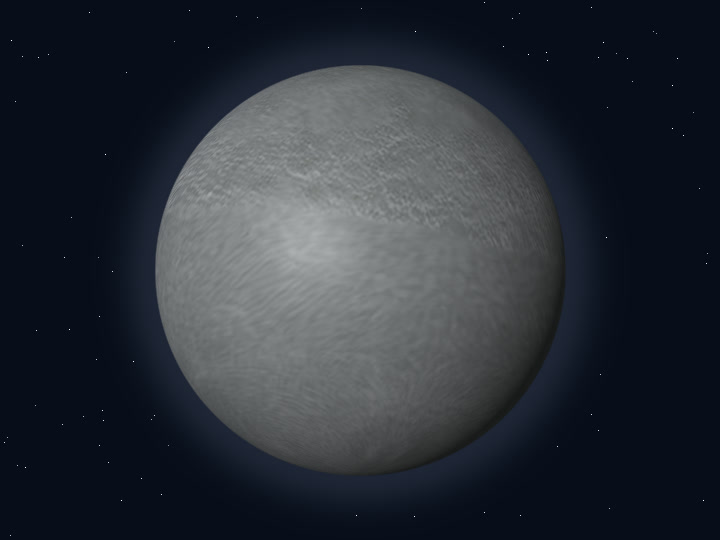
\includegraphics[width=\linewidth,height=4.4cm,keepaspectratio]{imagini/globuri/umbriel.jpg}\\[2pt]
{\scriptsize\itshape\color{orbitarMuted} Vedere 3D a corpului ceresc (\textbf{Umbriel})}
&
\centering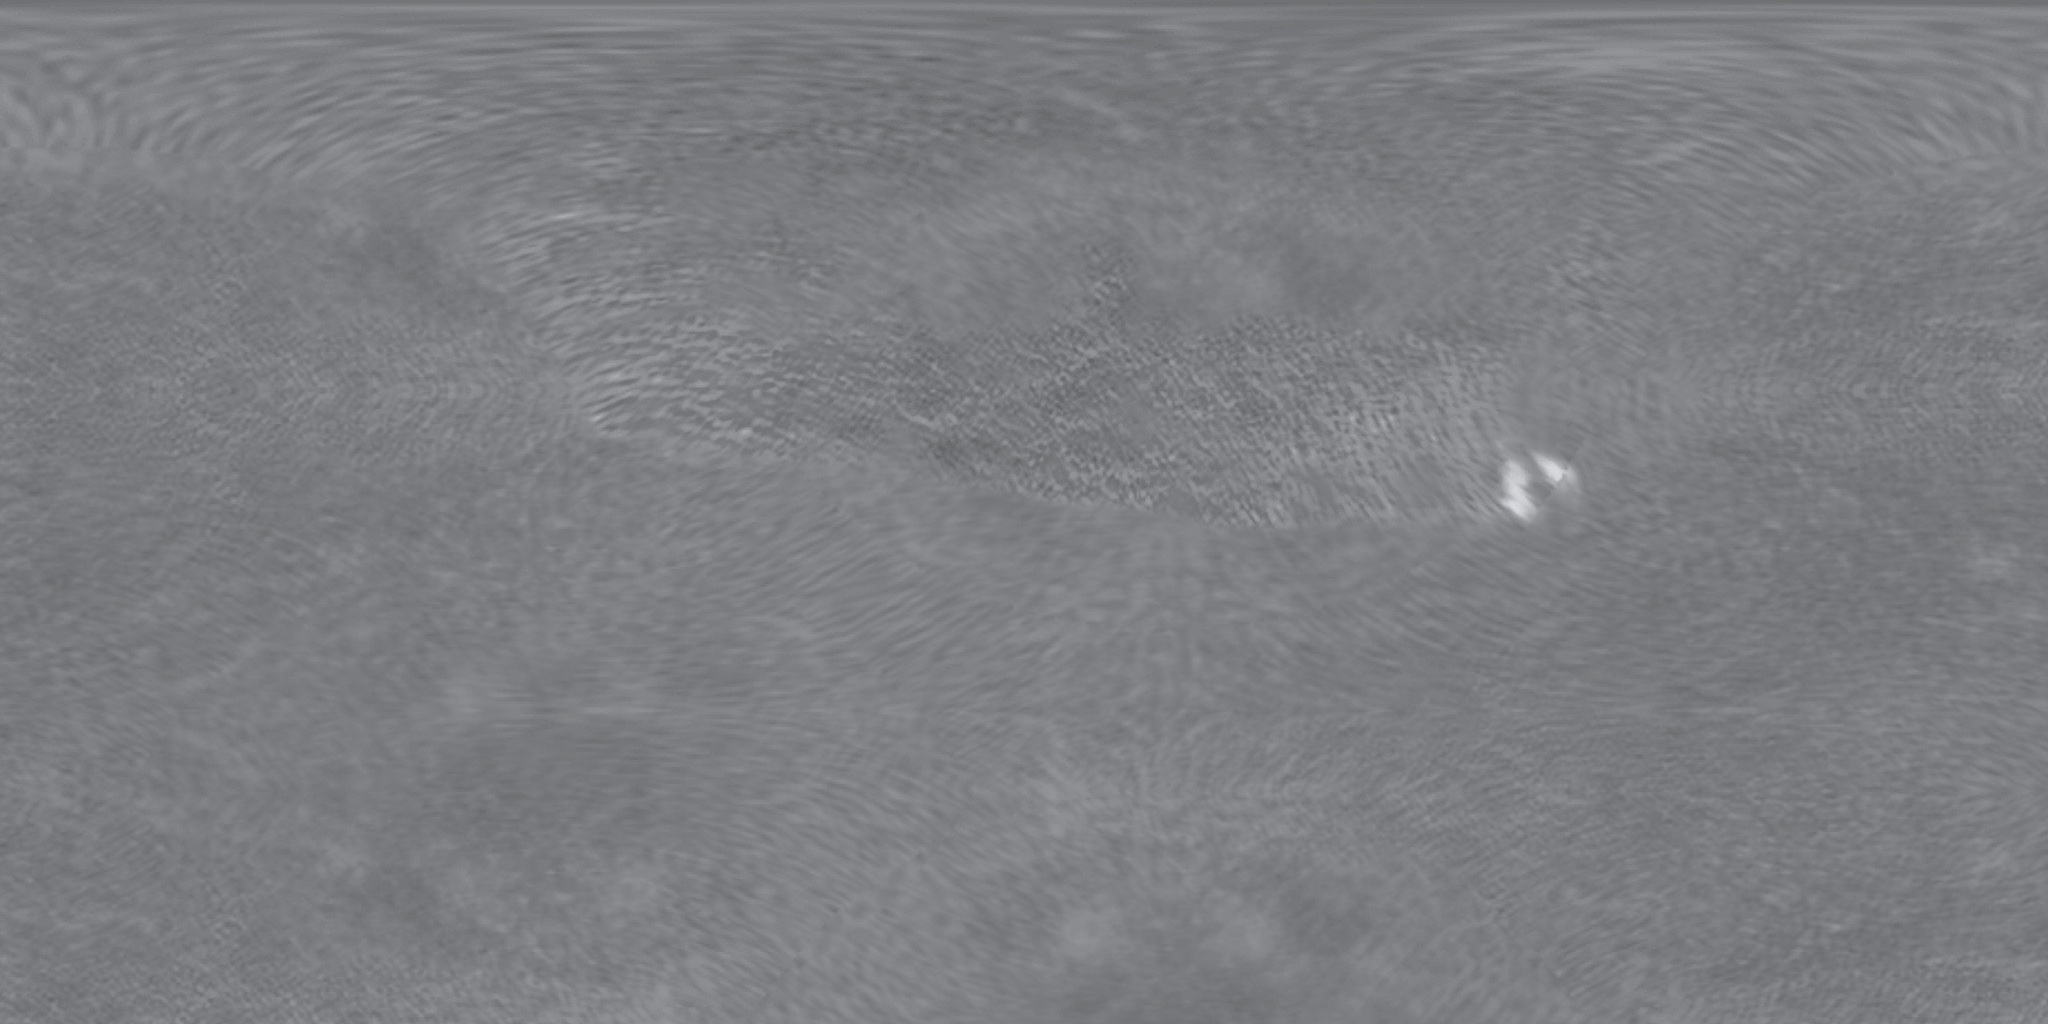
\includegraphics[width=\linewidth,height=4.4cm,keepaspectratio]{../public/textures/hd/umbriel_voyager.jpg}\\[2pt]
{\scriptsize\itshape\color{orbitarMuted} Planiglob desfășurat: Suprafața întunecată a lunii Umbriel și misteriosul inel luminos al craterului Wunda de la ecuator (NASA Voyager 2).}
\end{tabular}
\end{center}


\begin{tcolorbox}[orbitardata, title={\textbf{Repere esențiale: Umbriel}}]
\small
\begin{itemize}[leftmargin=1.4em, itemsep=2pt, topsep=2pt]
  \item \textbf{Clasificare și orbită:} Satelit Natural (Lună) (orbitează în jurul: \textbf{Uranus}) \quad$\bullet$\quad \textbf{Distanță:} 19,218 UA ($\approx$ 2.875 milioane de kilometri)
  \item \textbf{Dimensiuni și masă:} rază medie 584,7 de kilometri \quad$\bullet$\quad masă: 2,13e-4 $\times M_\oplus$
  \item \textbf{Gravitație și regim termic:} 0,023 $\times g_\oplus$ (0,23 m/s$^2$) \quad$\bullet$\quad temperatură medie: -198 $^\circ$C (înclinarea axei: Nespecificată)
  \item \textbf{Ciclu orbital și rotație:} perioadă orbitală (an): 4,144 zile pământești \quad$\bullet$\quad rotație (zi): 99,46 ore (4,14 zile pământești)
  \item \textbf{Durata călătoriei de pe Pământ:} cu viteza luminii ($1c$): \emph{2 ore și 30 de minute}; cu racheta ($50.000$ de kilometri pe oră): \emph{8 ani și jumătate}; cu avionul ($900$ de kilometri pe oră): \emph{345 de ani}; cu mașina ($100$ de kilometri pe oră): \emph{3.100 de ani}.
  \item \textbf{Repere de scară și curiozitate:} Inelul alb din craterul Wunda de pe Umbriel arată din spațiu ca o gogoașă glazurată luminoasă așezată chiar lângă ecuatorul unei lumi întunecate! Numele ei vine de la \guillemotleft{}Umbriel\guillemotright{}, un spirit melancolic al umbrelor dintr-un poem de Alexander Pope (și de la cuvântul latin \guillemotleft{}umbra\guillemotright{}!).
\end{itemize}
\end{tcolorbox}

\subsubsection*{Prezentare generală și profil astrofizic}
Descoperită în 1851 de William Lassell în aceeași zi cu Ariel, Umbriel are aproape aceeași dimensiune (diametru 1.169 de kilometri), dar o istorie geologică complet diferită: reflectă doar 16\% din lumină (jumătate față de Ariel) și păstrează o suprafață străveche, saturată cu cratere mari de impact. Umbriel este cea mai întunecată dintre lunile mari ale lui Uranus! Pe suprafața ei cenușie strălucește ca un far un inel alb misterios, aflat în craterul Wunda. Inelul alb din craterul Wunda de pe Umbriel arată din spațiu ca o gogoașă glazurată luminoasă așezată chiar lângă ecuatorul unei lumi întunecate!

\subsubsection*{Alcătuirea fizică și structura internă}
Privind în profunzimea sa, alcătuirea fizică este organizată pe mai multe straturi și regiuni distincte, fiecare având un rol bine definit în evoluția și dinamica acestui obiect cosmic. În primul rând se remarcă \textbf{Interior de gheață de apă și rocă (1,39 g/cm$^3$)}, care conține o proporție mai mare de gheață și mai puțină rocă decât Ariel, fără semne de refacere tectonică recentă a scoarței. În strânsă legătură cu această componentă se află \textbf{Suprafață străveche întunecată de toline și carbon}, acoperită de un strat subțire de material organic întunecat și cratere de până la 210 kilometri diametru (precum Skynd și Vuver). În completarea acestui ansamblu întâlnim \textbf{Craterul Wunda (131 de kilometri diametru)}, adăpostește pe podeaua sa un inel strălucitor lat de aproximativ 10 kilometri, format probabil din gheață pură de dioxid de carbon (CO$_2$) condensată în capcana termică a craterului.

\subsubsection*{Observații astronomice și istoricul explorării}
Fotografiată de sonda Voyager 2 în ianuarie 1986; este una dintre țintele principale pentru o viitoare sondă orbitală dedicată sistemului Uranus (Uranus Orbiter and Probe). Numele ei vine de la \guillemotleft{}Umbriel\guillemotright{}, un spirit melancolic al umbrelor dintr-un poem de Alexander Pope (și de la cuvântul latin \guillemotleft{}umbra\guillemotright{}!).

\vspace{6pt}
\begin{tcolorbox}[orbitarquiz, title={\textbf{Întrebare de verificare \#27: Umbriel}}]
\textbf{Ce detaliu strălucitor iese în evidență pe suprafața foarte întunecată a satelitului Umbriel?}
\begin{itemize}[leftmargin=2.2em, itemsep=2pt, topsep=4pt]
  \item[$\square$ \textbf{A.}] Inelul alb luminos de pe podeaua craterului ecuatorial Wunda
  \item[$\square$ \textbf{B.}] Un vulcan de sulf
  \item[$\square$ \textbf{C.}] Un ocean de metan lichid
  \item[$\square$ \textbf{D.}] Un inel planetar ca al lui Saturn
\end{itemize}
\vspace{2pt}
{\footnotesize\color{orbitarMuted}\textbf{Răspuns corect:} \textbf{A} (Inelul alb luminos de pe podeaua craterului ecuatorial Wunda). \emph{Craterul Wunda conține un inel lat și foarte luminos (probabil gheață de dioxid de carbon sau gheață de apă curată expusă la impact), care contrastează puternic cu restul suprafeței întunecate a lui Umbriel.}}
\end{tcolorbox}
\clearpage


\subsection{Titania}
\label{sec:body-titania}
\vspace{-4pt}
{\large\itshape\color{orbitarAccent} Cea mai mare lună a planetei Uranus, brăzdată de canioane de gheață}\\[4pt]


\begin{center}
\begin{tabular}{@{}m{0.44\textwidth}@{\hspace{0.03\textwidth}}m{0.51\textwidth}@{}}
\centering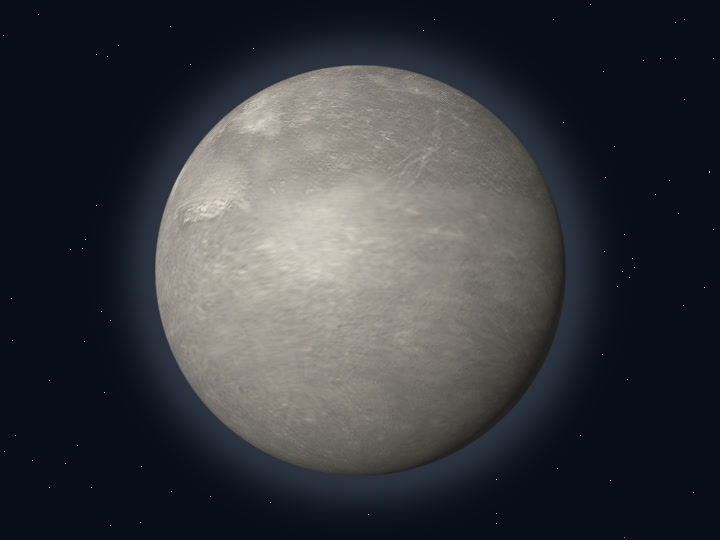
\includegraphics[width=\linewidth,height=4.4cm,keepaspectratio]{imagini/globuri/titania.jpg}\\[2pt]
{\scriptsize\itshape\color{orbitarMuted} Vedere 3D a corpului ceresc (\textbf{Titania})}
&
\centering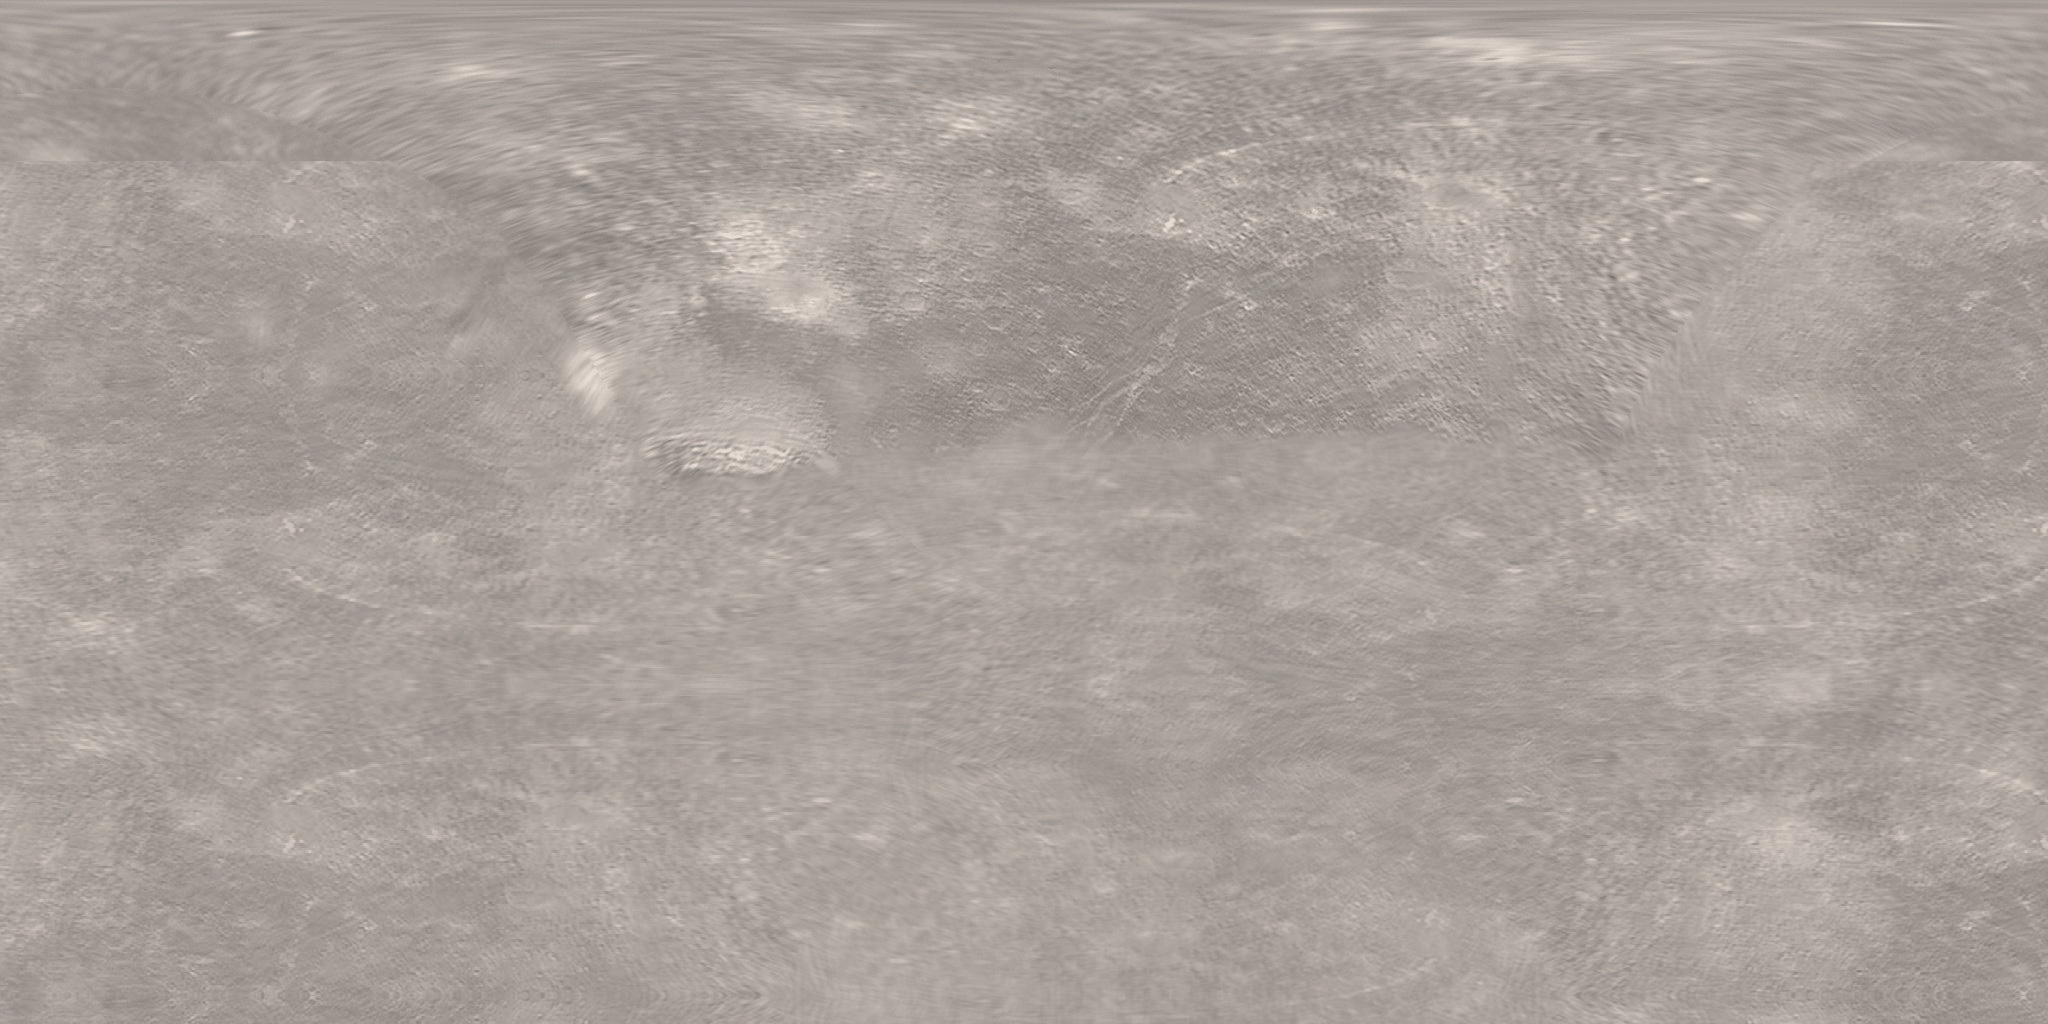
\includegraphics[width=\linewidth,height=4.4cm,keepaspectratio]{../public/textures/hd/titania_voyager.jpg}\\[2pt]
{\scriptsize\itshape\color{orbitarMuted} Planiglob desfășurat: Harta celei mai mari luni a lui Uranus, Titania, și a canionului tectonic Messina Chasmata (NASA Voyager 2).}
\end{tabular}
\end{center}


\begin{tcolorbox}[orbitardata, title={\textbf{Repere esențiale: Titania}}]
\small
\begin{itemize}[leftmargin=1.4em, itemsep=2pt, topsep=2pt]
  \item \textbf{Clasificare și orbită:} Satelit Natural (Lună) (orbitează în jurul: \textbf{Uranus}) \quad$\bullet$\quad \textbf{Distanță:} 19,218 UA ($\approx$ 2.875 milioane de kilometri)
  \item \textbf{Dimensiuni și masă:} rază medie 788,4 de kilometri \quad$\bullet$\quad masă: 5,90e-4 $\times M_\oplus$
  \item \textbf{Gravitație și regim termic:} 0,039 $\times g_\oplus$ (0,38 m/s$^2$) \quad$\bullet$\quad temperatură medie: -203 $^\circ$C (înclinarea axei: Nespecificată)
  \item \textbf{Ciclu orbital și rotație:} perioadă orbitală (an): 8,706 zile pământești \quad$\bullet$\quad rotație (zi): 208,94 ore (8,71 zile pământești)
  \item \textbf{Durata călătoriei de pe Pământ:} cu viteza luminii ($1c$): \emph{2 ore și 30 de minute}; cu racheta ($50.000$ de kilometri pe oră): \emph{8 ani și jumătate}; cu avionul ($900$ de kilometri pe oră): \emph{345 de ani}; cu mașina ($100$ de kilometri pe oră): \emph{3.100 de ani}.
  \item \textbf{Repere de scară și curiozitate:} La fel ca majoritatea sateliților lui Uranus, Titania poartă numele unui personaj din piesele lui William Shakespeare, și anume Regina Zânelor! Canionul Messina Chasmata de pe Titania este atât de lung încât s-ar întinde din România până în Spania!
\end{itemize}
\end{tcolorbox}

\subsubsection*{Prezentare generală și profil astrofizic}
Descoperită de William Herschel în 1787 (în aceeași noapte cu Oberon), Titania este al optulea satelit ca mărime din Sistemul Solar (diametru de 1.578 de kilometri). Orbitează în planul ecuatorial înclinat la 98$^\circ$ al lui Uranus, având anotimpuri extreme de câte 42 de ani. Titania este regina lunilor lui Uranus și cea mai mare dintre ele! Este o lume rece de gheață și stâncă, tăiată de un canion uriaș numit Messina Chasmata. La fel ca majoritatea sateliților lui Uranus, Titania poartă numele unui personaj din piesele lui William Shakespeare, și anume Regina Zânelor!

\subsubsection*{Alcătuirea fizică și structura internă}
Privind în profunzimea sa, alcătuirea fizică este organizată pe mai multe straturi și regiuni distincte, fiecare având un rol bine definit în evoluția și dinamica acestui obiect cosmic. În primul rând se remarcă \textbf{Nucleu stâncos (66\% din rază)}, care conține silicați și compuși organici, reprezentând aproximativ jumătate din masa satelitului. În strânsă legătură cu această componentă se află \textbf{Manta de gheață de apă}, unde când interiorul a înghețat și s-a dilatat în trecut, scoarța a crăpat formând falii gigantice. În completarea acestui ansamblu întâlnim \textbf{Messina Chasmata și Bazinul Gertrude}, sistem de grabene tectonice lung de 1.492 de kilometri și un crater de impact de 326 de kilometri diametru.

\subsubsection*{Observații astronomice și istoricul explorării}
Fotografiată de sonda Voyager 2 în ianuarie 1986; ocultațiile stelare au arătat că poate avea o atmosferă extrem de fină de dioxid de carbon. Canionul Messina Chasmata de pe Titania este atât de lung încât s-ar întinde din România până în Spania!

\vspace{6pt}
\begin{tcolorbox}[orbitarquiz, title={\textbf{Întrebare de verificare \#28: Titania}}]
\textbf{De unde provin numele sateliților planetei Uranus, precum Titania și Miranda?}
\begin{itemize}[leftmargin=2.2em, itemsep=2pt, topsep=4pt]
  \item[$\square$ \textbf{A.}] Din mitologia egipteană
  \item[$\square$ \textbf{B.}] Din operele literare ale lui William Shakespeare și Alexander Pope
  \item[$\square$ \textbf{C.}] De la numele râurilor din Europa
  \item[$\square$ \textbf{D.}] De la numele unor rachete
\end{itemize}
\vspace{2pt}
{\footnotesize\color{orbitarMuted}\textbf{Răspuns corect:} \textbf{B} (Din operele literare ale lui William Shakespeare și Alexander Pope). \emph{Spre deosebire de celelalte planete ale căror luni poartă nume din mitologia greco-romană, lunile lui Uranus sunt numite după personaje din Shakespeare și Pope.}}
\end{tcolorbox}
\clearpage


\subsection{Oberon}
\label{sec:body-oberon}
\vspace{-4pt}
{\large\itshape\color{orbitarAccent} Cea mai exterioară lună mare a lui Uranus, cu craterul Hamlet și un munte de 11 kilometri}\\[4pt]


\begin{center}
\begin{tabular}{@{}m{0.44\textwidth}@{\hspace{0.03\textwidth}}m{0.51\textwidth}@{}}
\centering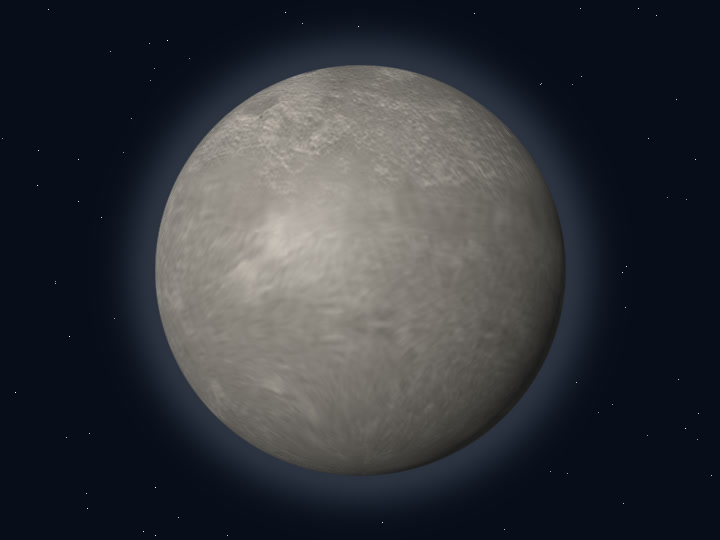
\includegraphics[width=\linewidth,height=4.4cm,keepaspectratio]{imagini/globuri/oberon.jpg}\\[2pt]
{\scriptsize\itshape\color{orbitarMuted} Vedere 3D a corpului ceresc (\textbf{Oberon})}
&
\centering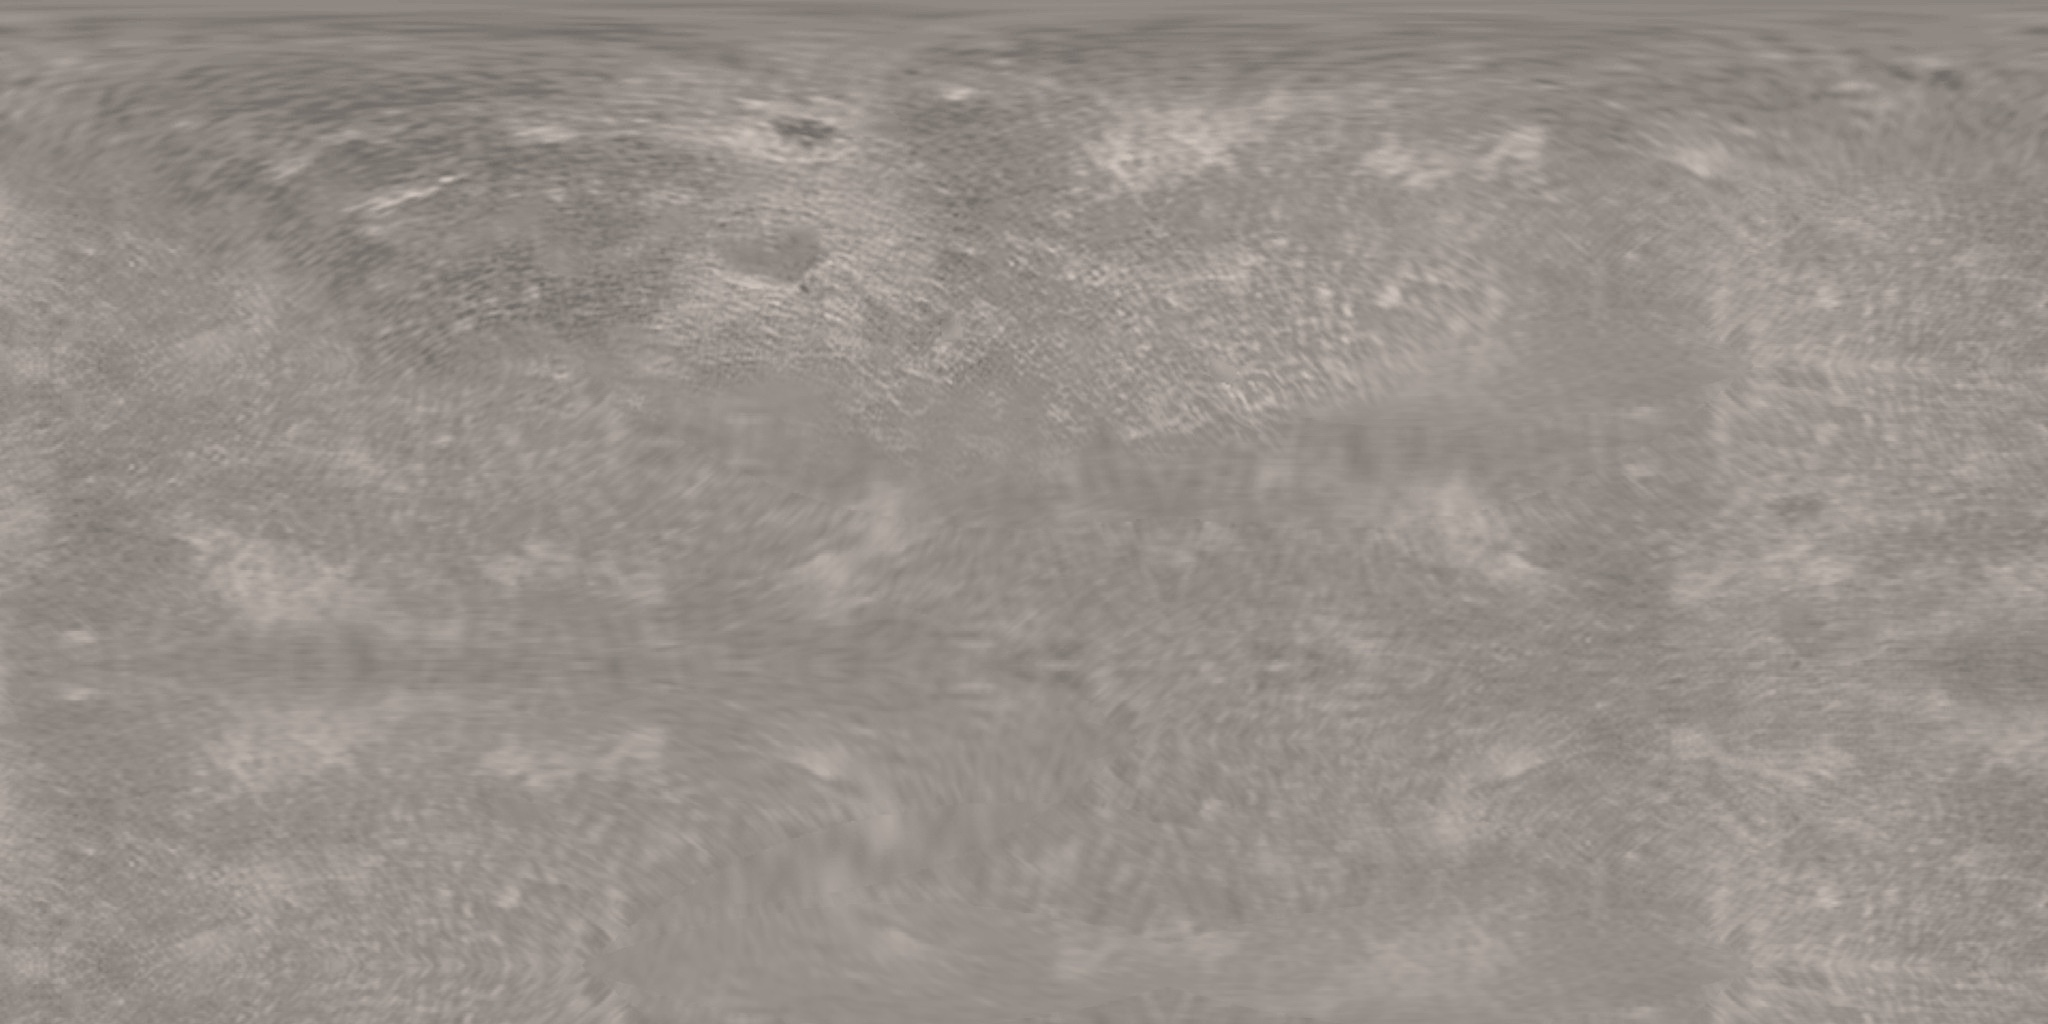
\includegraphics[width=\linewidth,height=4.4cm,keepaspectratio]{../public/textures/hd/oberon_voyager.jpg}\\[2pt]
{\scriptsize\itshape\color{orbitarMuted} Planiglob desfășurat: Harta celei mai exterioare luni mari a lui Uranus, Oberon, cu craterul Hamlet și razele sale de gheață (NASA Voyager 2).}
\end{tabular}
\end{center}


\begin{tcolorbox}[orbitardata, title={\textbf{Repere esențiale: Oberon}}]
\small
\begin{itemize}[leftmargin=1.4em, itemsep=2pt, topsep=2pt]
  \item \textbf{Clasificare și orbită:} Satelit Natural (Lună) (orbitează în jurul: \textbf{Uranus}) \quad$\bullet$\quad \textbf{Distanță:} 19,218 UA ($\approx$ 2.875 milioane de kilometri)
  \item \textbf{Dimensiuni și masă:} rază medie 761,4 de kilometri \quad$\bullet$\quad masă: 5,05e-4 $\times M_\oplus$
  \item \textbf{Gravitație și regim termic:} 0,035 $\times g_\oplus$ (0,34 m/s$^2$) \quad$\bullet$\quad temperatură medie: -198 $^\circ$C (înclinarea axei: Nespecificată)
  \item \textbf{Ciclu orbital și rotație:} perioadă orbitală (an): 13,463 zile pământești \quad$\bullet$\quad rotație (zi): 323,12 ore (13,46 zile pământești)
  \item \textbf{Durata călătoriei de pe Pământ:} cu viteza luminii ($1c$): \emph{2 ore și 30 de minute}; cu racheta ($50.000$ de kilometri pe oră): \emph{8 ani și jumătate}; cu avionul ($900$ de kilometri pe oră): \emph{345 de ani}; cu mașina ($100$ de kilometri pe oră): \emph{3.100 de ani}.
  \item \textbf{Repere de scară și curiozitate:} La marginea globului lui Oberon, sonda Voyager 2 a fotografiat un munte uriaș care se înalță la 11 kilometri deasupra orizontului, fiind mai înalt decât muntele Everest! Multe dintre craterele lui Oberon poartă nume de eroi din piesele lui Shakespeare: Hamlet, Othello, Macbeth, Lear și Romeo!
\end{itemize}
\end{tcolorbox}

\subsubsection*{Prezentare generală și profil astrofizic}
Descoperită de William Herschel la 11 ianuarie 1787 (în aceeași noapte cu Titania), Oberon este al zecelea satelit ca mărime din Sistemul Solar (diametru de 1.522,8 kilometri). Alcătuită în proporții egale din gheață de apă și rocă (densitate 1,63 g/cm$^3$), are o suprafață intens craterizată și canioane tectonice (Mommur Chasma). Oberon este Regele Zânelor și a doua lună ca mărime a lui Uranus! Se rotește cel mai departe de planetă dintre cele cinci luni mari și are cratere cu raze luminoase de gheață. La marginea globului lui Oberon, sonda Voyager 2 a fotografiat un munte uriaș care se înalță la 11 kilometri deasupra orizontului, fiind mai înalt decât muntele Everest!

\subsubsection*{Alcătuirea fizică și structura internă}
Privind în profunzimea sa, alcătuirea fizică este organizată pe mai multe straturi și regiuni distincte, fiecare având un rol bine definit în evoluția și dinamica acestui obiect cosmic. În primul rând se remarcă \textbf{Nucleu stâncos și manta de gheață (50\% rocă, 50\% gheață)}, care poate păstra la limita dintre nucleu și manta un strat subțire de ocean lichid bogat în amoniac. În strânsă legătură cu această componentă se află \textbf{Craterul Hamlet (206 kilometri diametru) și Othello}, cratere mari de impact înconjurate de raze luminoase de gheață proaspătă, dar având podeaua acoperită cu material criovulcanic întunecat. În completarea acestui ansamblu întâlnim \textbf{Muntele de la limb (aproximativ 11 kilometri înălțime) și Mommur Chasma}, un pisc central colosal observat în profil pe marginea discului de Voyager 2 și un canion tectonic lung de 537 de kilometri.

\subsubsection*{Observații astronomice și istoricul explorării}
Fotografiată de sonda Voyager 2 în ianuarie 1986 de la o distanță de 470.600 de kilometri. Multe dintre craterele lui Oberon poartă nume de eroi din piesele lui Shakespeare: Hamlet, Othello, Macbeth, Lear și Romeo!

\vspace{6pt}
\begin{tcolorbox}[orbitarquiz, title={\textbf{Întrebare de verificare \#29: Oberon}}]
\textbf{Ce formațiune spectaculoasă a observat sonda Voyager 2 ridicându-se pe marginea orizontului (limbul) satelitului Oberon?}
\begin{itemize}[leftmargin=2.2em, itemsep=2pt, topsep=4pt]
  \item[$\square$ \textbf{A.}] Un munte de aproximativ 11 kilometri înălțime (probabil piscul central al unui mare bazin de impact)
  \item[$\square$ \textbf{B.}] Un ocean de apă caldă
  \item[$\square$ \textbf{C.}] Un inel de praf
  \item[$\square$ \textbf{D.}] O furtună de nisip
\end{itemize}
\vspace{2pt}
{\footnotesize\color{orbitarMuted}\textbf{Răspuns corect:} \textbf{A} (Un munte de aproximativ 11 kilometri înălțime (probabil piscul central al unui mare bazin de impact)). \emph{În imaginile Voyager 2, pe limbul sud-estic al lui Oberon se profilează un munte înalt de aproximativ 11 kilometri, mai înalt decât Everestul de pe Pământ.}}
\end{tcolorbox}
\clearpage


\section{Neptun}
\label{sec:body-neptune}
\vspace{-4pt}
{\large\itshape\color{orbitarAccent} Planeta albastră a vânturilor supersonice}\\[4pt]


\begin{center}
\begin{tabular}{@{}m{0.44\textwidth}@{\hspace{0.03\textwidth}}m{0.51\textwidth}@{}}
\centering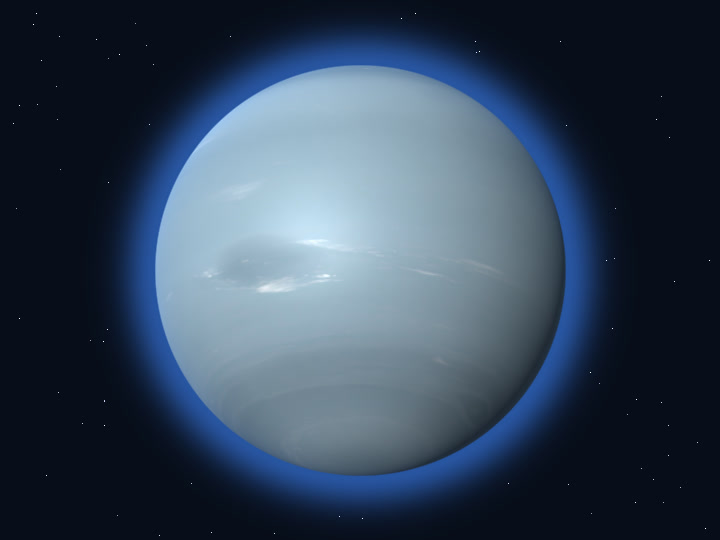
\includegraphics[width=\linewidth,height=4.4cm,keepaspectratio]{imagini/globuri/neptune.jpg}\\[2pt]
{\scriptsize\itshape\color{orbitarMuted} Vedere 3D a corpului ceresc (\textbf{Neptun})}
&
\centering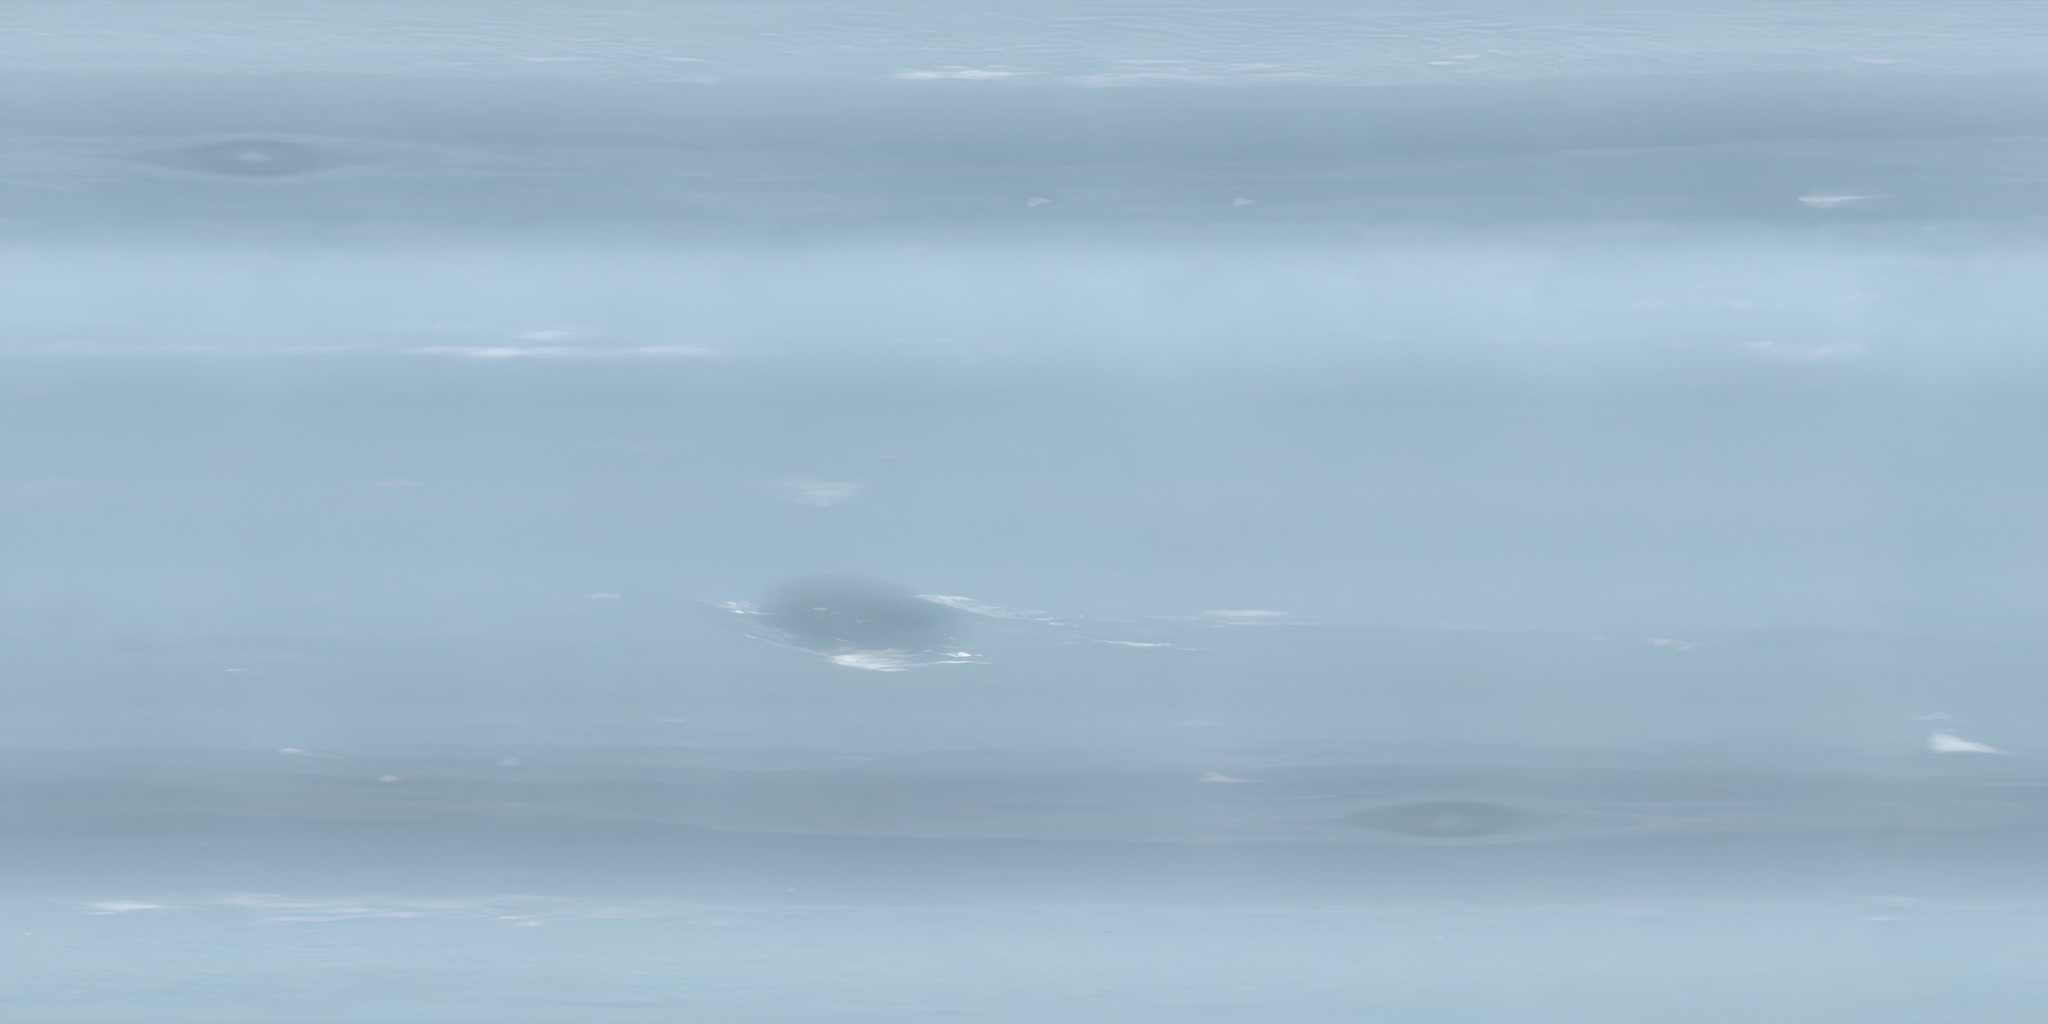
\includegraphics[width=\linewidth,height=4.4cm,keepaspectratio]{../public/textures/hd/neptune_voyager.jpg}\\[2pt]
{\scriptsize\itshape\color{orbitarMuted} Planiglob desfășurat: Harta atmosferei azurii și a furtunilor supersonice de pe Neptun, cartografiată de NASA Voyager 2.}
\end{tabular}
\end{center}


\begin{tcolorbox}[orbitardata, title={\textbf{Repere esențiale: Neptun}}]
\small
\begin{itemize}[leftmargin=1.4em, itemsep=2pt, topsep=2pt]
  \item \textbf{Clasificare și orbită:} Gigant de Gheață \quad$\bullet$\quad \textbf{Distanță:} 30,110 UA ($\approx$ 4.504 milioane de kilometri)
  \item \textbf{Dimensiuni și masă:} rază medie 24.622 de kilometri \quad$\bullet$\quad masă: 17,150 $\times M_\oplus$
  \item \textbf{Gravitație și regim termic:} 1,140 $\times g_\oplus$ (11,18 m/s$^2$) \quad$\bullet$\quad temperatură medie: -200 $^\circ$C (înclinarea axei: 28,32$^\circ$)
  \item \textbf{Ciclu orbital și rotație:} perioadă orbitală (an): 60.182 zile ($\approx$ 164,77 ani pământești) \quad$\bullet$\quad rotație (zi): 16,11 ore (0,67 zile pământești)
  \item \textbf{Durata călătoriei de pe Pământ:} cu viteza luminii ($1c$): \emph{4 ore și 10 minute}; cu racheta ($50.000$ de kilometri pe oră): \emph{12 ani (Voyager 2)}; cu avionul ($900$ de kilometri pe oră): \emph{550 de ani}; cu mașina ($100$ de kilometri pe oră): \emph{4.950 de ani}.
  \item \textbf{Repere de scară și curiozitate:} Neptun este de 30 de ori mai departe de Soare decât Pământul, astfel că acolo Soarele pare doar o stea foarte strălucitoare! De când a fost descoperit în anul 1846, Neptun a reușit să facă o singură tură completă în jurul Soarelui (în 2011)!
\end{itemize}
\end{tcolorbox}

\subsubsection*{Prezentare generală și profil astrofizic}
Neptun a fost prima planetă a cărei existență a fost prezisă prin calcul matematic (Urbain Le Verrier și John Couch Adams) înainte de a fi observată prin telescop în 1846. Deși primește de 900 de ori mai puțină energie solară decât Pământul, are cea mai dinamică meteorologie dintre giganți. Neptun este cea mai îndepărtată planetă mare de la Soare! Are culoarea unui ocean adânc și vânturi atât de rapide încât depășesc viteza sunetului. Neptun este de 30 de ori mai departe de Soare decât Pământul, astfel că acolo Soarele pare doar o stea foarte strălucitoare!

\subsubsection*{Alcătuirea fizică și structura internă}
Privind în profunzimea sa, alcătuirea fizică este organizată pe mai multe straturi și regiuni distincte, fiecare având un rol bine definit în evoluția și dinamica acestui obiect cosmic. În primul rând se remarcă \textbf{Nucleu stâncos}, cu o masă apropiată de cea a Pământului, la temperaturi de aproximativ 5.000 $^\circ$C. În strânsă legătură cu această componentă se află \textbf{Manta ionică de apă, amoniac și metan}, unde la adâncimi mari, presiunea poate descompune metanul în cristale de diamant. În completarea acestui ansamblu întâlnim \textbf{Atmosferă dinamică}, nori înalți de metan înghețat și vânturi care ating 2.100 kilometri pe oră.

\subsubsection*{Observații astronomice și istoricul explorării}
Survolată de sonda Voyager 2 în august 1989 și observată în infraroșu de Telescopul Spațial James Webb. De când a fost descoperit în anul 1846, Neptun a reușit să facă o singură tură completă în jurul Soarelui (în 2011)!

\vspace{6pt}
\begin{tcolorbox}[orbitarquiz, title={\textbf{Întrebare de verificare \#30: Neptun}}]
\textbf{Cum a fost descoperită planeta Neptun în anul 1846?}
\begin{itemize}[leftmargin=2.2em, itemsep=2pt, topsep=4pt]
  \item[$\square$ \textbf{A.}] Cu ochiul liber în Antichitate
  \item[$\square$ \textbf{B.}] Prin calcule matematice bazate pe perturbațiile orbitei lui Uranus
  \item[$\square$ \textbf{C.}] De către sonda Voyager 2
  \item[$\square$ \textbf{D.}] În timpul unei eclipse solare
\end{itemize}
\vspace{2pt}
{\footnotesize\color{orbitarMuted}\textbf{Răspuns corect:} \textbf{B} (Prin calcule matematice bazate pe perturbațiile orbitei lui Uranus). \emph{Matematicienii au observat că Uranus nu urma exact orbita calculată și au dedus poziția unei planete necunoscute care îl atrăgea gravitațional.}}
\end{tcolorbox}
\clearpage


\subsection{Triton}
\label{sec:body-triton}
\vspace{-4pt}
{\large\itshape\color{orbitarAccent} Marea lună înghețată a lui Neptun, cu gheizere de azot și orbită inversă}\\[4pt]


\begin{center}
\begin{tabular}{@{}m{0.44\textwidth}@{\hspace{0.03\textwidth}}m{0.51\textwidth}@{}}
\centering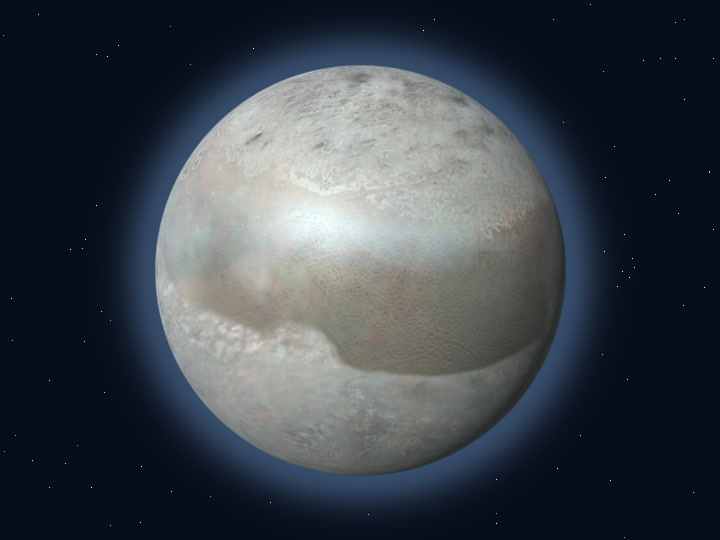
\includegraphics[width=\linewidth,height=4.4cm,keepaspectratio]{imagini/globuri/triton.jpg}\\[2pt]
{\scriptsize\itshape\color{orbitarMuted} Vedere 3D a corpului ceresc (\textbf{Triton})}
&
\centering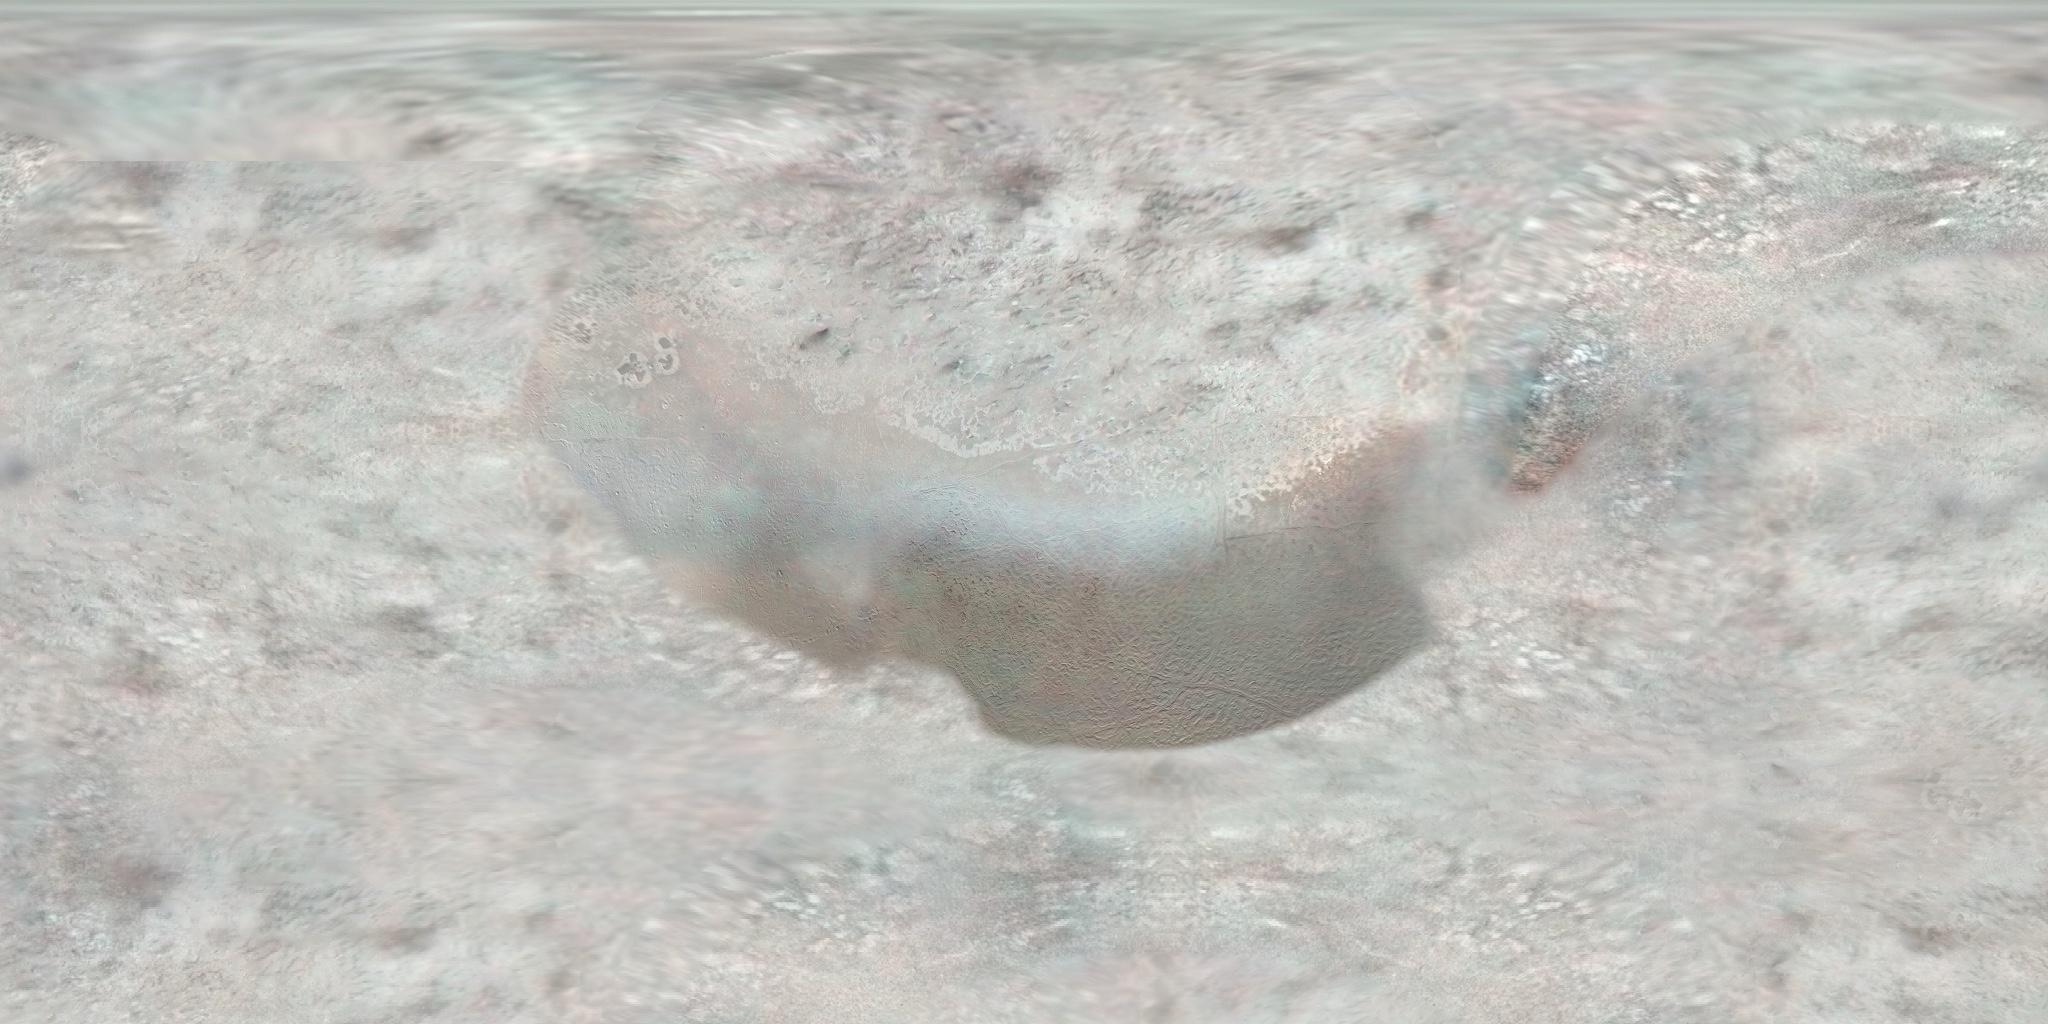
\includegraphics[width=\linewidth,height=4.4cm,keepaspectratio]{../public/textures/hd/triton_voyager.jpg}\\[2pt]
{\scriptsize\itshape\color{orbitarMuted} Planiglob desfășurat: Terenul de tip \quotedblbase{}coajă de pepene galben\textquotedblright{} și calota de azot înghețat cu gheizere de pe Triton (NASA Voyager 2).}
\end{tabular}
\end{center}


\begin{tcolorbox}[orbitardata, title={\textbf{Repere esențiale: Triton}}]
\small
\begin{itemize}[leftmargin=1.4em, itemsep=2pt, topsep=2pt]
  \item \textbf{Clasificare și orbită:} Satelit Natural (Lună) (orbitează în jurul: \textbf{Neptun}) \quad$\bullet$\quad \textbf{Distanță:} 30,110 UA ($\approx$ 4.504 milioane de kilometri)
  \item \textbf{Dimensiuni și masă:} rază medie 1.353,4 de kilometri \quad$\bullet$\quad masă: 0,004 $\times M_\oplus$
  \item \textbf{Gravitație și regim termic:} 0,079 $\times g_\oplus$ (0,77 m/s$^2$) \quad$\bullet$\quad temperatură medie: -235 $^\circ$C (înclinarea axei: Nespecificată)
  \item \textbf{Ciclu orbital și rotație:} perioadă orbitală (an): 5,877 zile pământești (Orbită retrogradă!) \quad$\bullet$\quad rotație (zi): 141,00 ore (Rotație retrogradă!)
  \item \textbf{Durata călătoriei de pe Pământ:} cu viteza luminii ($1c$): \emph{4 ore și 10 minute}; cu racheta ($50.000$ de kilometri pe oră): \emph{12 ani (Voyager 2)}; cu avionul ($900$ de kilometri pe oră): \emph{550 de ani}; cu mașina ($100$ de kilometri pe oră): \emph{4.950 de ani}.
  \item \textbf{Repere de scară și curiozitate:} O mare parte din suprafața lui Triton are denivelări ciudate care arată exact ca coaja unui pepene galben! Triton este singura lună mare din Sistemul Solar care merge \guillemotleft{}pe contrasens\guillemotright{} și se învârte în jurul lui Neptun în sens invers față de rotația planetei!
\end{itemize}
\end{tcolorbox}

\subsubsection*{Prezentare generală și profil astrofizic}
Descoperită în 1846 de William Lassell la doar 17 zile după descoperirea lui Neptun, Triton este al șaptelea satelit ca mărime din Sistemul Solar (mai mare decât Pluto). Orbita sa retrogradă demonstrează că a fost o planetă pitică din Centura Kuiper capturată gravitațional de Neptun. Triton este cea mai mare lună a lui Neptun și una dintre cele mai reci lumi din Sistemul Solar! Are gheizere care aruncă nori negri de azot înghețat până la 8 kilometri înălțime. O mare parte din suprafața lui Triton are denivelări ciudate care arată exact ca coaja unui pepene galben!

\subsubsection*{Alcătuirea fizică și structura internă}
Privind în profunzimea sa, alcătuirea fizică este organizată pe mai multe straturi și regiuni distincte, fiecare având un rol bine definit în evoluția și dinamica acestui obiect cosmic. În primul rând se remarcă \textbf{Nucleu mare stâncos-metalic}, densitate ridicată (2,06 g/cm$^3$) și posibil ocean subglaciar menținut lichid de căldura radiogenică și mareică. În strânsă legătură cu această componentă se află \textbf{Teren \guillemotleft{}coajă de pepene galben\guillemotright{} (Bubembe Regio)}, regiune unică formată prin diapirismul gheții (ridicarea și coborârea lentă a blocurilor de gheață). În completarea acestui ansamblu întâlnim \textbf{Calotă polară rozalie de azot și criovulcani}, gheizere active de azot gazos și praf întunecat, plus o atmosferă subțire de azot cu nori la 235 $^\circ$C sub zero.

\subsubsection*{Observații astronomice și istoricul explorării}
Explorată în premieră la 25 august 1989 de sonda Voyager 2, care a fotografiat în direct erupțiile gheizerelor sale polare. Triton este singura lună mare din Sistemul Solar care merge \guillemotleft{}pe contrasens\guillemotright{} și se învârte în jurul lui Neptun în sens invers față de rotația planetei!

\vspace{6pt}
\begin{tcolorbox}[orbitarquiz, title={\textbf{Întrebare de verificare \#31: Triton}}]
\textbf{Ce ne indică faptul că satelitul Triton se rotește în sens invers (retrograd) în jurul lui Neptun?}
\begin{itemize}[leftmargin=2.2em, itemsep=2pt, topsep=4pt]
  \item[$\square$ \textbf{A.}] Că nu s-a format lângă Neptun, ci a fost un corp din Centura Kuiper capturat de gravitația planetei
  \item[$\square$ \textbf{B.}] Că Neptun nu are gravitație
  \item[$\square$ \textbf{C.}] Că este făcut din fier
  \item[$\square$ \textbf{D.}] Că se îndepărtează de Soare
\end{itemize}
\vspace{2pt}
{\footnotesize\color{orbitarMuted}\textbf{Răspuns corect:} \textbf{A} (Că nu s-a format lângă Neptun, ci a fost un corp din Centura Kuiper capturat de gravitația planetei). \emph{Un satelit format împreună cu planeta sa orbitează în sensul rotației planetei; orbita retrogradă a lui Triton dovedește că a fost capturat din Centura Kuiper.}}
\end{tcolorbox}
\clearpage

